\documentclass[a4paper,12pt]{article}

% -------------------------------------------------
% Pacchetti essenziali importanti!
% -------------------------------------------------
\usepackage[utf8]{inputenc}
\usepackage[T1]{fontenc}
\usepackage{lmodern}
\usepackage{amsmath,amsfonts,amssymb}
\usepackage{graphicx}
\usepackage{listings,xcolor}
\usepackage{enumitem}
\usepackage{hyperref}
\usepackage{float}
\usepackage{listings}
\usepackage{xcolor}
\usepackage{listings}
\definecolor{mylightgray}{rgb}{0.97,0.97,0.97}
\hypersetup{
	colorlinks=true,
	linkcolor=blue,
	urlcolor=blue,
	citecolor=blue
}

\lstset{
	language=Matlab,
	backgroundcolor=\color{mylightgray},
	basicstyle=\ttfamily\footnotesize,
	keywordstyle=\color{blue}\bfseries,
	commentstyle=\color{green!60!black}\itshape,
	stringstyle=\color{red},
	numbers=left,
	numberstyle=\tiny,
	stepnumber=1,
	numbersep=5pt,
	frame=single,
	breaklines=true,
	showstringspaces=false,
	tabsize=4,
	captionpos=b
}
% -------------------------------------------------

\begin{document}
	
	% ---------- Frontespizio (pag. 1) ----------------
	\title{\textbf{Numerical Optimization for Large Scale Problems}\\
	\vspace{0.5em}\huge\textbf{Report}
	\author{
		Di Battista Simona — 302689%\\
		\and
		Rostagno Andrea — 349152\\
			}
	
	\vspace{0.5cm}
	\large Assignment on Unconstrained Optimization}
	%%\date{\today}
	\maketitle
	\thispagestyle{empty}   % (facoltativo) niente numero in frontespizio
	\newpage                % <-- salto di pagina: l’indice parte da qui
	
	% ---------- Indice (pag. 2) ----------------------
	\pagenumbering{roman}   % numeri romani per indice (i, ii, iii…)
	\tableofcontents
	\newpage                % nuovo salto: inizia il testo
	
	% ---------- Testo principale (da pag. 3) ---------
	\pagenumbering{arabic}  % riparte da 1 con numeri arabi
	
	% =================================================
	\section{Introduction}
	
	The goal of this project is to implement and compare two numerical methods for unconstrained optimization: the Modified Newton method and the Nelder-Mead method. \\
	
	First these algorithms are tested on the standard 2-dimensional Rosenbrock function using two different initial conditions, in order to validate their implementation. Subsequently, they are applied to three benchmark problems selected from the test set for unconstrained optimization proposed in \cite{luksan1999}. \\
	
	For benchmark problems, in accordance with the assignment instructions,  the Nelder-Mead method is tested in low dimensions \( n = 10, 26, 50 \), while the Modified Newton method is evaluated on \( n = 10^3, 10^4, 10^5 \). Furthermore, for each test function and each method, a fixed starting point $\bar{x}$ suggested in \cite{luksan1999} is used, together with 10 uniformly randomly generated starting points, sampled in the hypercube $[\bar{x}_{1}-1,\bar{x}_{1}+1]\times\dots\times[\bar{x}_{n}-1,\bar{x}_{n}+1] \subset \mathbb{R}^{n}$. Performance is assessed in terms of number of successful runs, total iterations, CPU time. Also an experimental rate of convergence is computed, starting from the definition of rate of convergence. First it was defined $e^{(k)} = x^{(k)} - x^{\star}$, where $x^{\star}$ is the optimal minimizer; since the value of the optimal minimizer is not known a priori, it is replaced in the formula by the last available approximation, obtaining $e^{(k)} \approx x^{(k)} - x^{(k-1)}$. For $k$ large enough
	\[
	\frac{\left\|e^{(k+1)}\right\|}{\left\|e^{(k)}\right\|} \approx \left\| \frac{e^{(k)}}{e^{(k-1)}} \right\|^{\rho} \Rightarrow \rho \approx \frac{\log\left(\left\|e^{(k+1)}\right\|\big/\left\|e^{(k)}\right\|\right)}{\log\left(\left\|e^{(k)}\right\|\big/\left\|e^{(k-1)}\right\|\right)}.
	\]
	Ultimately, the experimental convergence rate is determined by implementing the following formula:
	\[
	\rho \approx \frac{\log\left(\|x^{(k+1)} - x^{(k)}\|\big/\|x^{(k)} - x^{(k-1)}\|\right)}{\log\left(\|x^{(k)} - x^{(k-1)}\|\big/\|x^{(k-1)} - x^{(k-2)}\|\right)}.
	\]
		Each starting point is associated with a run, considered successful when the algorithm satisfies a prescribed stopping criterion within a certain maximum number of iterations, depending on the method. These details will be described better in the next sections. Moreover, in the case of Modified Newton method, in addition to exact gradients and hessians, finite differences approximations are employed with different step sizes and types of increment. \\
	
	%\vspace{0.5em}
	The next sections describe the implemented methods and the test problems in detail, followed by a discussion of the experimental results, cost analysis, and final remarks.
		
	\vspace{1em}
	
	
	\vspace{1em}	
		
	\newpage
	\subsection{Modified Newton Method}
	
	The Modified Newton method is a variant of the classical Newton method. At each iteration it computes a search direction $p^{(k)}$ by solving the linear system
	\[
	H_{mod}^{(k)} \thinspace p^{(k)} = -\nabla f(x^{(k)}), \qquad 
	\]
	involving a modified version of the hessian matrix, computed as follow: 
	\[
	H_{mod}^{(k)} = H^{(k)} + E^{(k)} .
	\]
	This modification is to ensure the positive definiteness of the hessian, so it is not necessarily computed. The update rule is
	\[
	x^{(k+1)} = x^{(k)} + \alpha^{(k)} p^{(k)}, \qquad 
	\]
	where \( \alpha^{(k)} \) is determined in the code by a backtracking line search, governed by the Armijo condition
	\[
	f(x^{(k)} + \alpha^{(k)} p^{(k)}) \leq f(x^{(k)}) + c \alpha^{(k)} \nabla f(x^{(k)})^\top p^{(k)}.
	\]
	The algorithm attempts a full step \( \alpha^{(k)} = 1 \) first, and then reduces it geometrically until the condition is met or a maximum number of trials is reached. \\
	
	\noindent In our implemetation:
	\begin{enumerate}
	\item $E^{(k)} = \tau I$. A modified Cholesky factorization is applied (Algorithm 6.3 ), that attempts to factor \( H^{(k)} \approx LL^\top \) and adds the regularization shift \( \tau I \), if needed.
	The procedure starts with \( \tau = 0 \), and doubles it iteratively until the factorization succeeds, ensuring positive definiteness of the hessian at each step.
	\item $\rho = 0.5$  and ${c} = 10^{-4}$ are default parameters in the Armijo condition.
	\item max\_backtracking\_iter $= 10$ is the maximum number of trials in the backtracking procedure. This value was chosen to prevent the stepsize alpha from becoming too small, and thus not adding more information than the current approximation of $x$.
	\end{enumerate}
%\vspace{0.5cm}	
\noindent	Additionally, when testing problems with structure (such as banded functions), some components of the gradient and direction vectors are padded to preserve compatibility with the structure of the objective function and to avoid dimension mismatch. Finally, the following stopping criteria were considered:
	\begin{itemize}
		\item \( \|\nabla f(x^{(k+1)})\|_\infty \leq \texttt{tol} \): the norm of the gradient computed in the new approximation is sufficiently small (below a required tolerance). If this criterion is met, the algorithm has reached a stationary point for the function to be minimized; 
		\item \( |f(x^{(k+1)}) - f(x^{(k)})| \leq \texttt{tol} \cdot \max(1, |f(x^{(k)})|) \): the relative functional decrement is sufficiently small (below a required tolerance). Such a criterion is introduced to prevent the algorithm from proceeding in an unnecessarily costly number of iterations, which do not significantly improve the function (as in the case of the Banded Trigonometric problem);
		\item \( f(x^{(k+1)}) \leq \texttt{tol} \): the value of the function computed in the new approximation is sufficiently small (below a required tolerance). This stopping criterion is introduced in the case of functions whose minimum value is 0 (as in the case of Extended Rosenbrock and Generalized Broyden problems). 
	\end{itemize}    
	
	\noindent The algorithm breaks before reaching the maximum number of iterates, as soon as one of the previous conditions --checked in that order-- is met. In the study of all benchmark problems, when Modified Newton method is applied, each individual execution, associated with a specific initial point, was considered a success if the algorithm breaks since the gradient is close to zero, that is, if the algorithm reaches a stationary point of the function.  
	%\vspace{0.5em}
	
	\subsubsection{Finite differences approximations}
	Within the elaborate, where possible, the finite differences method was implemented for the computation of first--and second--order derivatives. In the code, this variant is found in the Modified Newton method, which requires calculation of both the gradient and the hessian of the function to be minimized. Recalling that Nelder-Mead is a "zero-order" method, this part does not involve the use of finite differences. \\
	
	The gradient approximation is obtained using the centered finite differences formula. In fact, although this is more expensive than forward and backward formulas, it offers a more accurate approximation of the required value. Considering $f: \mathbb{R}^{n} \xrightarrow{}\mathbb{R}$ and $\nabla f: \mathbb{R}^{n} \xrightarrow{}\mathbb{R}^{n}$, with 
	\[
	\nabla f(x) =  \bigg( \frac{\partial f}{\partial x_{1}}(x),\dots,\frac{\partial f}{\partial 
		x_{n}}(x)\bigg),
	\]
	using centered finite differences for the approximated gradient, we obtain
	\begin{equation}\label{eq1}
		\frac{\partial f}{\partial x_{i}}(x) \approx \frac{f(x+he_{i}) - f(x-he_{i})}{2h}, \quad i = 1,\dots,n.	
	\end{equation}
	
	Instead, in the hessian matrix $\nabla^{2}f \in \mathbb{R}^{n,n}$\\
	
	\begin{center}
		$\nabla^{2}f(x) =$
		$\begin{pmatrix}
			
			\frac{\partial^{2}f}{\partial x_{1}^{2}}(x) & \dots & \frac{\partial^{2} f}{\partial x_{1}\partial x_{n}}(x)\\
			\vdots & \ddots &\vdots \\
			\frac{\partial^{2} f}{\partial x_{n}\partial x_{1}}(x) & \dots & \frac{\partial^{2}f}{\partial x_{n}^{2}}(x)
		\end{pmatrix}$, \\
	\end{center}
	
	%\noindent diagonal elements are estimated as
	%%	\frac{\partial^{2}f}{\partial x_{i}^{2}}(x) \approx \frac{f(x+he_{i})-2f(x)+f(x-he_{i})}{h^{2}},	\end{equation}
	
	\noindent each entry is obtained using the following calculus:
	
	\begin{equation}\label{eq3}
		\frac{\partial^{2} f}{\partial x_{i}\partial x_{j}}(x) \approx \frac{f(x+he_{i}+he_{j}) - f(x+he_{i})-f(x+he_{j})+f(x)}{h^{2}}.
	\end{equation}
	
	The code implement the finite differences approximations, passing via handles the extra parameters \texttt{h} and \( \texttt{type} \). In particular
	\begin{itemize}
		\item \texttt{h}: is a parameter equal to \(10^{-k} \), for \( k = 2, 4, 6, 8, 10, 12 \);
		\item \texttt{type}: is a parameter which indicates the typology of the increment. If type = 1 a variant of the increment scaled componentwise as \( h_i = 10^{-k} \cdot |x_i| \) is used (this ensures reasonable accuracy and robustness when computing derivatives in high dimensions), otherwise default increment with \( h_i = 10^{-k}\) is employed. 
	\end{itemize}
	
		Since application of the Modified Newton method to large benchmak problems $(n = 10^{3},10^{4},10^{5})$ is required in the assignment, it was not possible to implement the formulas as presented, but it was necessary to make extensive use of each test function's structure and sparsity of each hessian matrix. Alternatively, the time to run the algorithms would have been excessive. In each of the sections regarding individual benchmark problems, it is detailed how these features were exploited in order to obtain reasonable results. 
	
	
		
	\vspace{1em}
	
	
	\vspace{1em}	
		
	\newpage
	\subsection{Nelder--Mead Method}
	
	The Nelder--Mead algorithm is a popular derivative--free optimization method designed to minimize a real-valued function \( f: \mathbb{R}^n \to \mathbb{R} \) without relying on gradient or hessian informations. The algorithm operates by iteratively updating a simplex—a geometric figure composed of \( n+1 \) vertices in \( \mathbb{R}^n \)—based on function evaluations at its vertices.
	
	At initialization, the algorithm constructs the simplex by perturbing the initial guess \( x^{(0)} \) along the canonical directions with a small fixed step size. At each iteration $k$, the vertices are sorted according to their function values, in such a way that
	\[
	f(x^{(k)}_{1})\leq f(x^{(k)}_{2})\leq\dots\leq f(x^{(k)}_{n+1}).
	\]
	Then the algorithm computes the centroid \( \bar{x} \) of the best \( n \) vertices (excluding the worst one $x^{(k)}_{n+1}$), and applies the following operations:
	\begin{itemize}
		\item \textbf{Reflection:} the worst vertex is reflected through the centroid to produce a new trial point $x^{(k)}_{R}$. If $f(x^{(k)}_{1})\leq f(x^{(k)}_{R})<f(x^{(k)}_{n})$, then $x^{(k)}_{R}$ is accepted in the new simplex in place of $x^{(k)}_{n+1}$.
		\item \textbf{Expansion:} if $f(x^{(k)}_{R}) < f(x^{(k)}_{1})$, the reflected point significantly improves the function, so an expansion is attempted further along the reflection direction producing the point $x^{(k)}_{E}$. If $f(x^{(k)}_{E}) < f(x^{(k)}_{R})$, then $\tilde{x}^{(k+1)}_{n+1} = x^{(k)}_{E}$, otherwise $\tilde{x}^{(k+1)}_{n+1} = x^{(k)}_{R}$.
		\item \textbf{Contraction:} if the reflection fails to improve, the algorithm attempts a contraction between the centroid and the worst vertex, producing the point $x^{(k)}_{C}$. 
		\item \textbf{Shrinkage:} if the contraction step is successful, then $\tilde{x}^{(k+1)}_{n+1} = x^{(k)}_{C}$, otherwise the entire simplex is shriked around the best vertex.
	\end{itemize}
	
	In our implementation default coefficients which are standard in the literature are used: \(\rho = 1\) (reflection parameter), \(\chi = 2 \) (expansion parameter), \( \gamma = 0.5 \) (contraction parameter), and \( \sigma = 0.5 \) (shrinkage parameter).\\
	
	Convergence is declared when one of the following stopping conditions is met:
	\begin{itemize}
		\item \(
		|f(x_{\max}) - f(x_{\min})| \leq \texttt{tol}:
		\) the maximum difference in function values across the simplex is sufficiently small (below a required tolerance);
		\item \(
		\max_{i=2,\dots,n+1} \|x^{(i)} - x^{(1)}\|_{\infty} \leq \texttt{tol}
		\): the maximum distance between simplex points is sufficiently small (below a required tolerance).
	\end{itemize}
	
	%The results are used primarily as a baseline reference for comparison with second-order methods.
	
	\vspace{1em}
	
	
	\vspace{1em}
	
	
	\newpage
	
	\section{Rosenbrock Function in Dimension 2}
	
	\subsection{Problem introduction}
	The Rosenbrock function is a well-known test case for unconstrained optimization. Its 2-dimensional version is defined as
	\[
	f(x_1,x_2) = 100(x_2 - x_1^2)^2 + (1 - x_1)^2,
	\]
	and features a curved valley with a global minimum \( f(x^\star) = 0 \) at \( x^\star = (1,1) \). Due to the narrow and curved shape of the valley, the problem is nontrivial for many first-order methods. \\
	
	We tested both the Modified Newton and Nelder–Mead algorithms using the two standard initial guesses required by the assignment:
	\[
	x^{(0)}_A = (1.2,\,1.2), \qquad x^{(0)}_B = (-1.2,\,1.0).
	\]\\
	
	\textbf{3D Visualization of the function:}
	\begin{figure}[htbp]
		\centering
		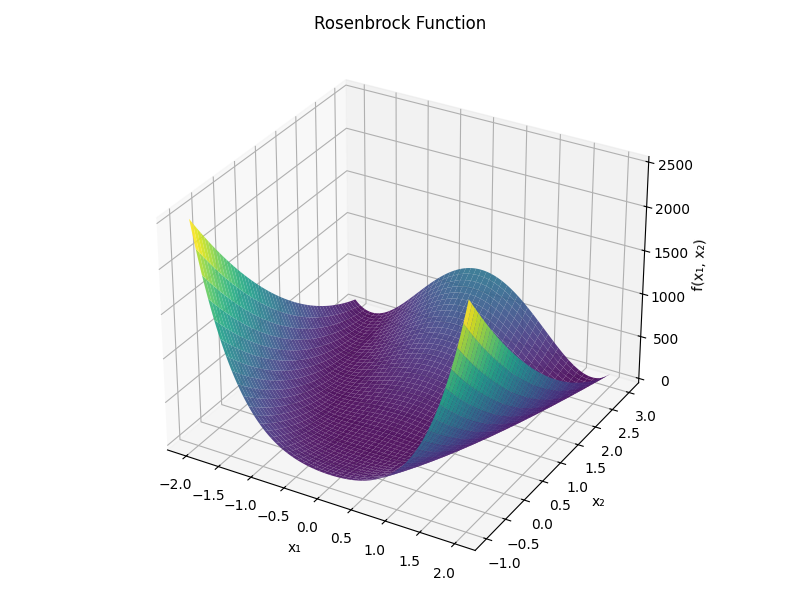
\includegraphics[width=0.7\textwidth]{../immagini/rosen3D_A.png}
		\caption{Surface plot of the Rosenbrock function over the domain $[-2, 2] \times [-1, 3]$. The function exhibits a narrow curved valley with a global minimum at $(1, 1)$, where $f(x) = 0$. This geometry makes it a standard benchmark for testing unconstrained optimization algorithms.}
		
		\label{fig:rosennewton}
	\end{figure}
	
	\vspace{1em}
	
	
	\vspace{1em}
	
	\newpage
	
	\subsection{Experimental results}
	This subsection discusses the results obtained for the minimization of the 2-dimensional Rosenbrock function, comparing the application of the  Modified Newton method and the Nelder--Mead method.\\
	
	
\begin{itemize}	
	\item \textbf{Modified Newton Method}:
	
	\begin{table}[H]
		\begin{tabular}{lllc}
			\hline
			Starting point  & Function minimum & Function minimizer    & Number of iterations \\ \hline
			\( x^{(0)}_A \) & 0.000000                 & $(1.000050,1.000083)$ & 6                    \\ \hline
			\( x^{(0)}_B \) & 0.000000         & $(0.999995,0.999990)$ & 21                   \\ \hline
		\end{tabular}
		\caption{The table highlights the convergence results associated with the application of the Modified Newton method. The analysis takes into account the starting point, the value of the minimum and the value of the minimizer reached, and the number of iterations that were required to achieve these results.}
	\end{table}
	
	\begin{figure}[htbp]
		\centering
		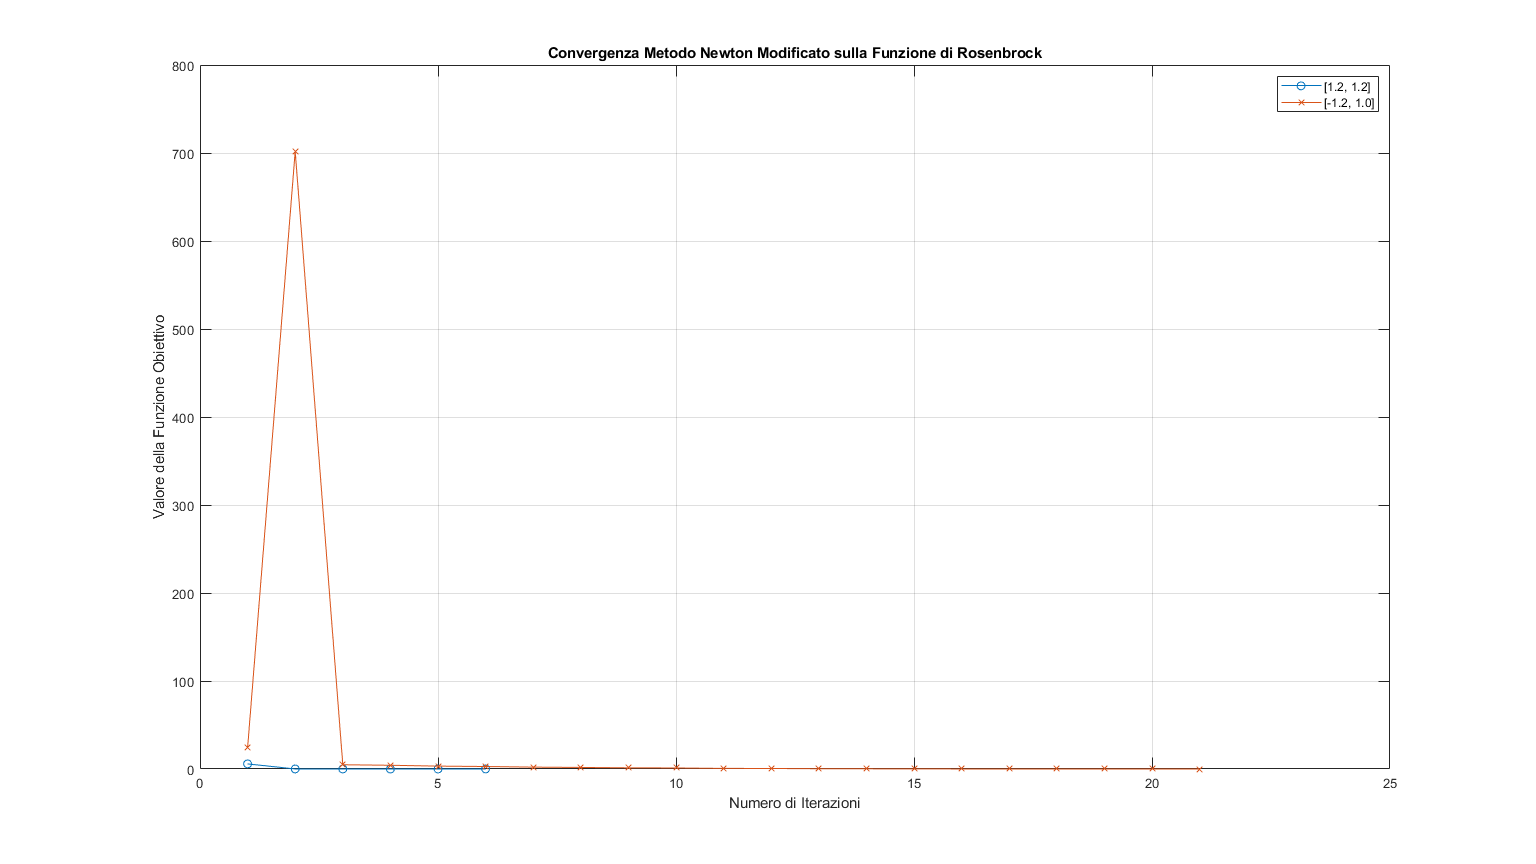
\includegraphics[width=0.7\textwidth]{../immagini/grafrosennewton.png}
		\caption{Convergence behaviour of the Modified Newton method on the Rosenbrock function starting from $x_{A}^{(0)} = [1.2, 1.2]$ and $x_{B}^{(0)} = [-1.2, 1.0]$.}
		\label{fig:rosennewton}
	\end{figure}
	\newpage
	\item 	\textbf{Nelder–Mead Method}:
	\begin{table}[H]
		\begin{tabular}{lllc}
			\hline
			Starting point  & Function minimum & Function minimizer    & Number of iterations \\ \hline
			\( x^{(0)}_A \) & 0.000000                 & $( (0.999741,0.999441)$ & 58                    \\ \hline
			\( x^{(0)}_B \) & 0.053018         & $( (1.222612,1.488895)$ & 29                   \\ \hline
		\end{tabular}
		\caption{The table highlights the convergence results associated with the application of the Nelder--Mead method. The analysis takes into account the starting point, the value of the minimum and the value of the minimizer reached, and the number of iterations that were required to achieve these results.}
	\end{table}
		
	\begin{figure}[htbp]
		\centering
		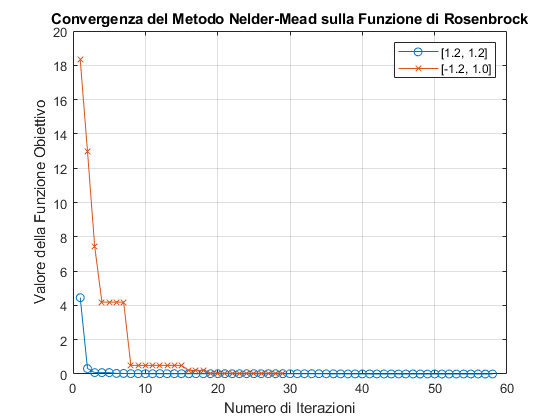
\includegraphics[width=0.8\textwidth]{../immagini/grafrosennelder.png}
		\caption{Convergence behaviour of the Nelder--Mead method on the Rosenbrock function starting from $x^{(0)}_{A} = [1.2, 1.2]$ and $x^{(0)}_{B} = [-1.2, 1.0]$.}
		\label{fig:rosennewton}
	\end{figure}
\end{itemize}
	 
	Although both methods converge starting from \( x^{(0)}_A \), the Modified Newton method reaches the solution significantly faster (6 iterations vs.\ 58). Starting from the more challenging initial point \( x^{(0)}_B \), the Modified Newton method converges reliably, while Nelder–Mead gets stuck in a suboptimal region, with higher final function value and fewer iterations. This fact confirms the advantage of second--order informations for curved valleys.
	
	

	
	\vspace{1em}
	
	
	\vspace{1em}
	
	
	 
	\newpage
	\section{Extended Rosenbrock Function}
	\subsection{Problem introduction}
	
	The Extended Rosenbrock function is an high-dimensional generalization of the classical Rosenbrock function. For even dimensions \( n \), it is defined as follow:
	\[
	F(x) = \frac{1}{2} \sum_{k=1}^{n} f_k^2(x), \qquad
	f_k(x) = 
	\begin{cases}
		10(x_k^2 - x_{k+1}), & \text{if } k \bmod 2 = 1 \\
		x_{k-1} - 1, & \text{if } k \bmod 2 = 0
	\end{cases}.
	\]
	
	This function is non--convex and features a narrow curved valley that makes optimization challenging in high dimensions. Its global minimum is \( f(x^\star) = 0 \) and its minimizer \( x^\star\) such that \( x^\star_{k} = 1, \hspace{0.1cm}\forall i = 1,\dots,n\). It is frequently used as a benchmark problem for large--scale unconstrained optimization algorithms, due to its scalability and pathological curvature.\\
	 
	In this chapter we are going to analyze the behaviour of both the Modified Newton and the Nelder–Mead methods, when they are applied to minimize the Extended Rosenbrock function. 
	The initial points suggested in the benchmark library  are $\bar{x} \in \mathbb{R}^{n}$ such that

		\begin{equation}
		\bar{x}_{k} =
		\begin{cases}
			-1.2 & \text{if} \quad k \bmod 2 = 1\\
			 \quad 1.0 & \text{if} \quad k \bmod 2 = 0
		\end{cases},
		\end{equation}
		
		 together with another 10 random initial points sampled uniformly in the hypercube $[\bar{x}_{1}-1,\bar{x}_{1}+1]\times\dots\times[\bar{x}_{n}-1,\bar{x}_{n}+1] \subset \mathbb{R}^{n}$, starting from $\bar{x}$.
	\newpage
	\begin{figure}[htbp]
		\centering
		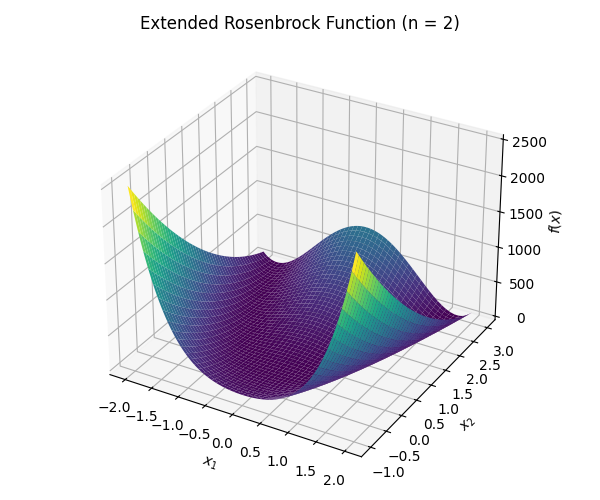
\includegraphics[width=0.6\textwidth]{../immagini/ext_rosen_3d.png}
		\caption{3D visualization of the Extended Rosenbrock function in dimension $n=2$. The global minimum lies at $(1,1)$, and the function exhibits a curved valley that becomes increasingly difficult to navigate in higher dimensions.}
		\label{fig:extrosen3d}
	\end{figure}
	
	\subsection{Modified Newton method}
	In this subsection are shown the results obtained from the minimization of the Extended Rosenbrock function using the Modified Newton method. The study includes both exact derivatives and derivatives computed by finite--differences approximations. Due to its tridiagonal structure, the hessian is stored and manipulated in sparse format; this choice drastically reduces memory requirements and computational cost (in both matrix factorization and Newton direction computation), allowing efficiently handle large--scale problems. Before presenting detailed outcomes, a general experimental setup is given:
	\begin{itemize}
		\item \texttt{n} $= 10^{3},10^{4},10^{5}$;
		\item \texttt{max\_iter} $= 5000$;
		\item \texttt{tol} $= 10^{-6}$.
	\end{itemize}
	
	\vspace{0.5cm}
	For each run, the following were tracked:
	\begin{itemize}
		\item number of iterations to convergence;
		\item CPU time;
		\item number of successful runs;
		\item experimental rate of convergence \(\rho\):
		\[
		\rho \approx \frac{\log\left(\|x^{(k+1)} - x^{(k)}\|\big/\|x^{(k)} - x^{(k-1)}\|\right)}{\log\left(\|x^{(k)} - x^{(k-1)}\|\big/\|x^{(k-1)} - x^{(k-2)}\|\right)}.
		\]
		\end{itemize}
	In correspondence with the randomly generated points, an average behavior of each of the previous catogories is reported. Furthermore, the code is designed to work also with finite--differences case,  and this variant is implemented thanks to the extra parameters 
	\begin{itemize}
		\item \texttt{h}: a parameter equal to \(10^{-k} \), for \( k = 2, 4, 6, 8, 10, 12 \);
		\item \texttt{type}: a parameter which indicates if the increment is scaled componentwise as \( h_i = 10^{-k} \cdot |x_i| \) or if it is a default increment such that \( h_i = 10^{-k}\). 
	\end{itemize}
	
	\noindent For this part, the several features were computed for each stepsize h.
	
	\subsubsection{Modified Newton method with exact derivatives}
		
	The Extended Rosenbrock function admits analytical expressions for both gradient and hessian in component--wise form. These are derived by exploiting the structure of the function and are used directly in the implementation for performance and accuracy. Specifically:
	
	\begin{itemize}
		\item each gradient's component is computed as:
		\[
		\frac{\partial F}{\partial x_k}(x) =
		\begin{cases}
			200(x_k^3 - x_k x_{k+1}) + (x_k - 1), & \text{if } k \bmod 2 = 1 \\
			-100(x_{k-1}^2 - x_k),               & \text{if } k \bmod 2 = 0
		\end{cases};
		\]
		
		\item each entry of the hessian is given by:
		\[
		\frac{\partial^2 F}{\partial x_k \partial x_j}(x) =
		\begin{cases}
			200(3x_k^2 - x_{k+1}) + 1, & \text{if } j = k,\ k \bmod 2 = 1 \\
			100,                      & \text{if } j = k,\ k \bmod 2 = 0 \\
			-200x_k,                  & \text{if } |k - j| = 1,\ k \bmod 2 = 1 \\
			0                       & \text{otherwise}
		\end{cases}.
		\]
		
	\end{itemize}
	
	

	%\vspace{1em}


	%\vspace{1em}
	
		
	%\newpage
	
	
	 \begin{center}
	 	\begin{table}
	 		\begin{tabular}{|c|c|c|c|c|c|}
	 			\hline
	 			\textbf{Dimension} & \textbf{Starting point} & \textbf{Iter} & \textbf{Time (s)} & \textbf{\(\rho\)} & \textbf{Success} \\
	 			\hline
	 			$10^3$ & $\bar{x}$         & 20   & 0.00 & 2.14 & 1/1 \\
	 			$10^3$ & Avg (10 pts)      & 25.3 & 0.01 & 2.02 & 10/10 \\
	 			\hline
	 			$10^4$ & $\bar{x}$         & 20   & 0.02 & 2.14 & 1/1 \\
	 			$10^4$ & Avg (10 pts)      & 25.4 & 0.05 & 1.96 & 10/10 \\
	 			\hline
	 			$10^5$ & $\bar{x}$         & 20   & 0.34 & 2.14 & 1/1 \\
	 			$10^5$ & Avg (10 pts)      & 26.0 & 0.74 & 1.37 & 10/10 \\
	 			\hline
	 		\end{tabular}
	 		\caption{The table highlights the convergence results associated with the application of the Modified Newton method with exact derivatives. The analysis takes into account the starting point (for the 10 random points an average behaviour is reported), the number of iterations that were required to achieve the result, the CPU time (s) and the rate of convergence $\rho$.}
	 		\label{table3}
	 	\end{table}
	 \end{center}
	 %\vspace{0.5em}
	 \paragraph{Experimental results.}All runs shown in table (\ref{table3}) were successful according to the stopping criterion related to the gradient (\( \|\nabla f(x^{(k)})\|_\infty \leq \texttt{tol}\)), and reached the known minimum \( f^\star = 0 \) up to machine precision. The number of iterations remains nearly constant across dimensions both for $\bar{x}$ and for the 10 random starting points, highlighting the scalability of Newton’s method when combined with sparse matrix storage. CPU time increases with \(n\), as expected due to the cost of Cholesky factorization on sparse tridiagonal matrices. The experimental convergence rate \(\rho\) remains close to quadratic (\(\rho \approx 2\)) for moderate dimensions, while it slightly drops for \(n=10^5\), possibly due to cumulative rounding errors.
	
	
	\begin{figure}[H]%[htbp]
		\centering
		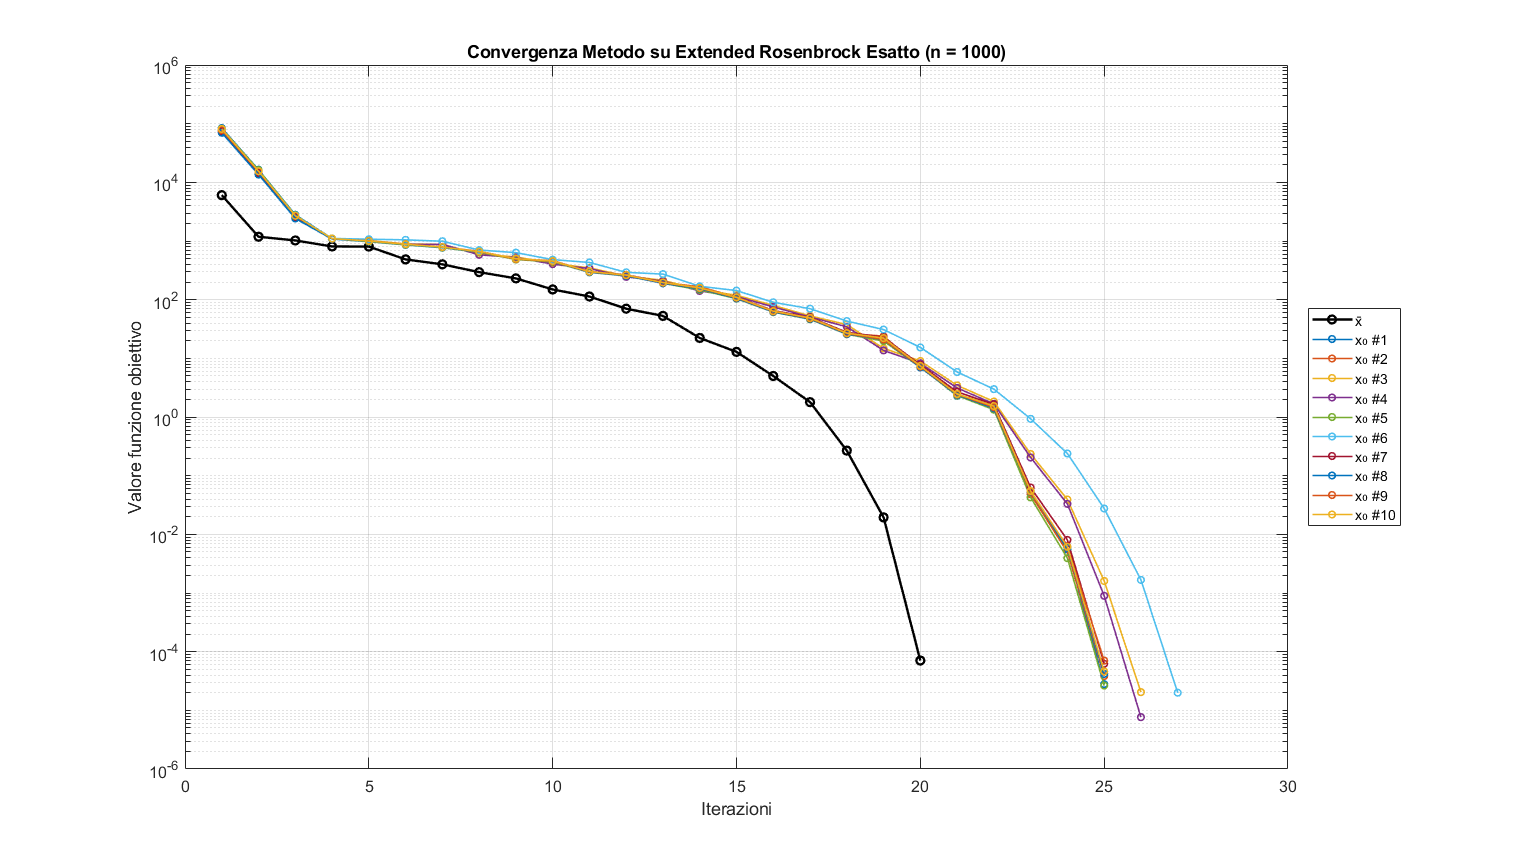
\includegraphics[width=0.85\textwidth]{../immagini/ext_1k.png}
		\caption{Convergence of the Modified Newton method with exact derivatives on the Extended Rosenbrock function for $n=1000$. Each curve corresponds to a different initial point. The method converges quadratically with stable behaviour across all tests.}
		\label{fig:extnewton_1k}
	\end{figure}
	
	\begin{figure}[H]%[htbp]
		\centering
		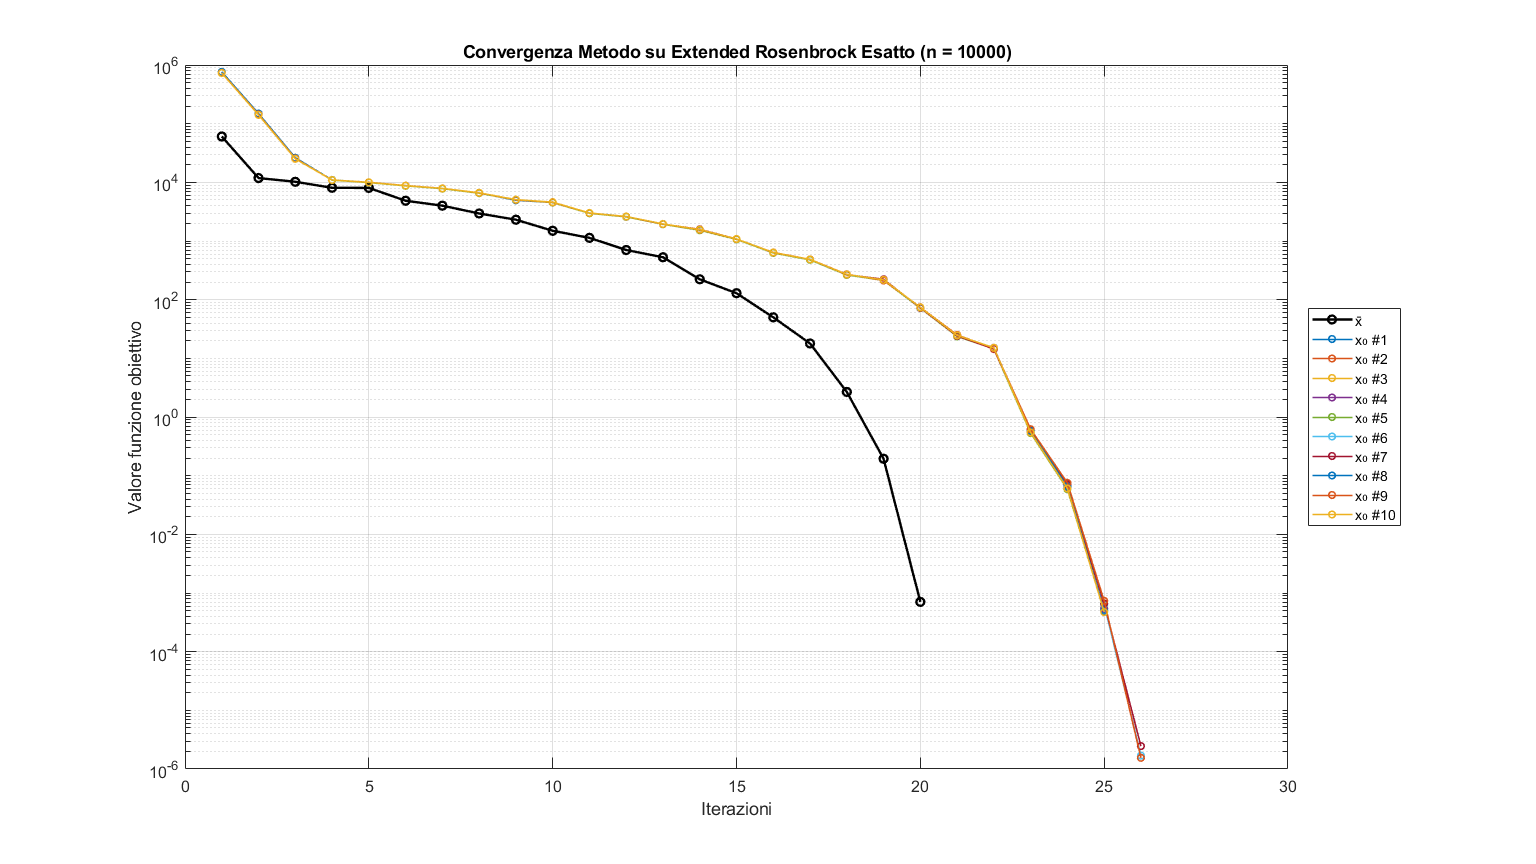
\includegraphics[width=0.85\textwidth]{../immagini/ext_10k.png}
		\caption{Convergence of the Modified Newton method on the Extended Rosenbrock function for $n=10\,000$. The method exhibits consistent quadratic convergence also in higher dimension.}
		\label{fig:extnewton_10k}
	\end{figure}
	
	\begin{figure}[H]%[htbp]
		\centering
		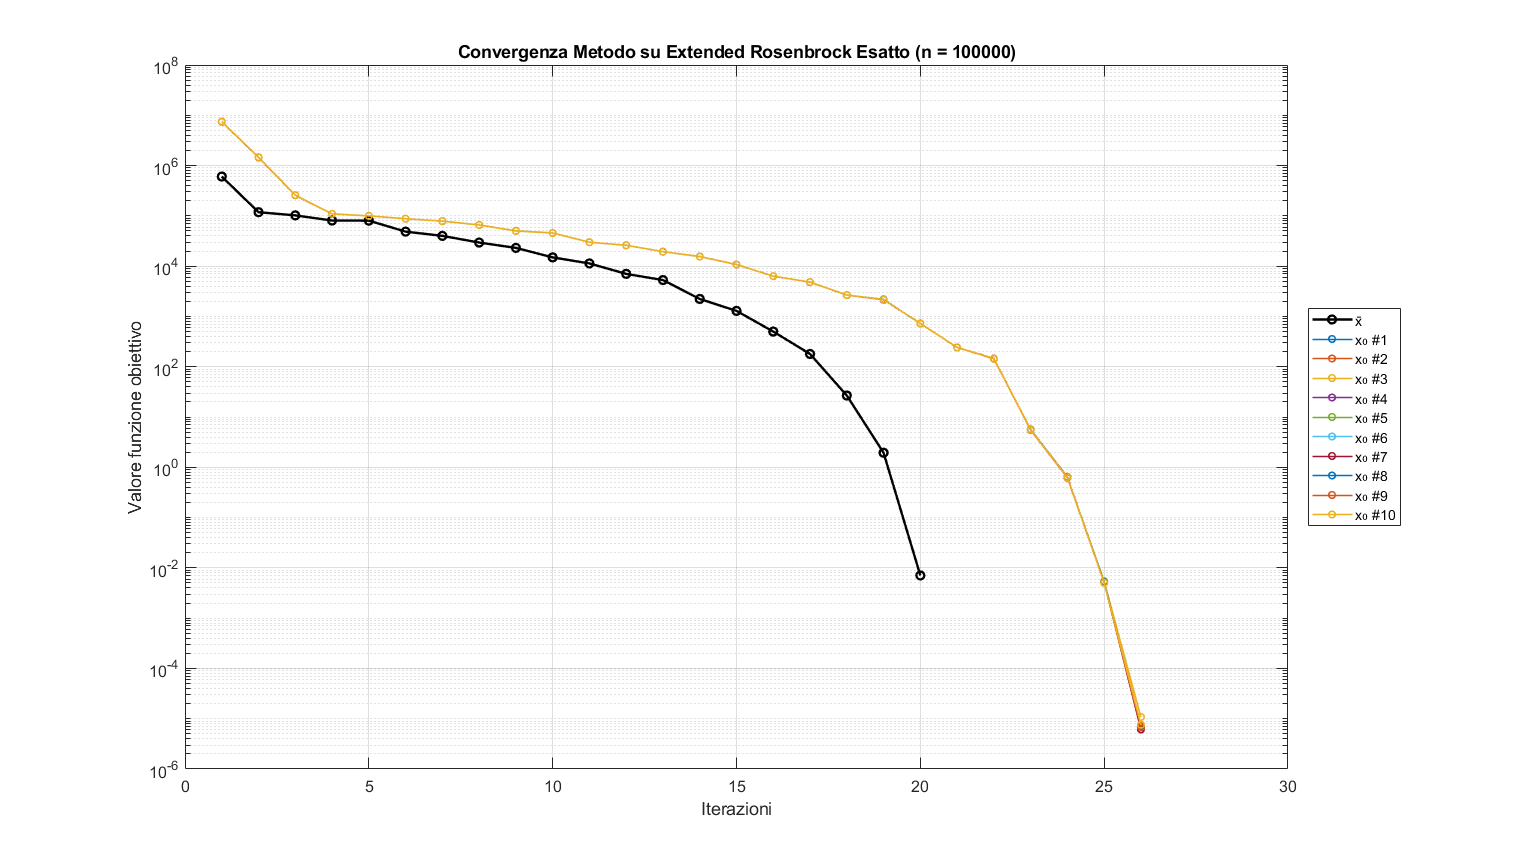
\includegraphics[width=0.85\textwidth]{../immagini/ext_100k.png}
		\caption{Convergence of the Modified Newton method on the Extended Rosenbrock function for $n=100\,000$. Despite the high dimensionality, the convergence remains stable with similar iteration counts.}
		\label{fig:extnewton_100k}
	\end{figure}
	
	\begin{figure}[H]%[htbp]
		\centering
		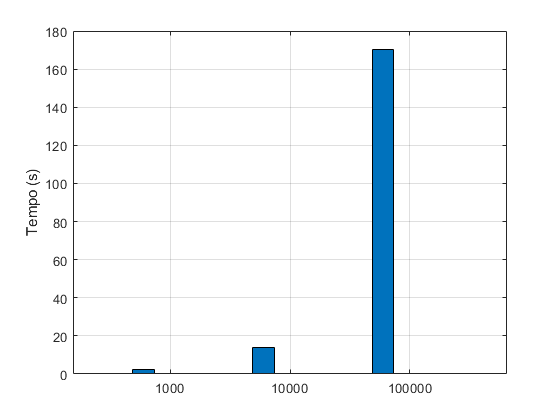
\includegraphics[width=0.6\textwidth]{../immagini/ext_time.png}
		\caption{Execution time (in seconds) of the Modified Newton method with exact derivatives for $n=10^3$, $10^4$ and $10^5$. The runtime grows approximately linearly with the problem size, confirming the efficiency of sparse matrix operations.}
		\label{fig:extnewton_times}
	\end{figure}
	
	\subsubsection{Modified Newton method with approximated derivatives}
	When exact gradients and hessians are not available, a common alternative is to approximate them using finite differences method. In our implementation, we manually built
	the approximations in component-wise form, exploiting the alternating structure of the Extended Rosenbrock function.
	\paragraph{Gradient approximation.}
	As we have seen in the introduction part, the gradient vector is computed using the centered finite differences formula (\ref{eq1}). Due to the structure of the function, only a small number of $f_{k}$ survive when computing the numerator in the formula. In particular, fixed $k$ as the component whose derivative is being approximated:
	
	\begin{equation}
	\frac{\partial F}{\partial x_{k}}(x) \approx	
	\begin{cases}
	\frac{\frac{1}{2}[f^{2}_{k}(x+he_{k}) + f^{2}_{k+1}(x+he_{k})] - \frac{1}{2}[f^{2}_{k}(x-he_{k}) + f^{2}_{k+1}(x-he_{k})]}{2h} & \text{if } k \bmod 2 = 1 \\
	
	\frac{\frac{1}{2}f^{2}_{k-1}(x+he_{k}) - \frac{1}{2}f^{2}_{k-1}(x-he_{k})}{2h} & \text{if } k \bmod 2 = 0
	
	\end{cases}	
		  .	
	\end{equation}
	
Thus, the finite-difference approximation of the gradient was implemented as:
\[
\frac{\partial F}{\partial x_k}(x) \approx 
\begin{cases}
	600x_k^2 - 100x_k x_{k+1} + \frac{1}{2}h + 350x_k^3 + 300hx_k^2, & \text{if } k \bmod 2 = 1 \\
	-100x_{k-1}^2 + 100x_k, & \text{if } k \bmod 2 = 0
\end{cases}.
\]
	
	\paragraph{Hessian approximation.}
	First, as seen in the previous section, we recall that the hessian matrix of the Extended Rosenbrock function has a tridiagonal structure. Then, appling the same proceeding as before, we can observe that function evaluations needed to compute diagonal entries of $\nabla^{2}F(x)$, differ only by the terms 
	 \[
	 \begin{cases}
	 	\frac{1}{2}[f^{2}_{k}(x) + f^{2}_{k+1}(x)]& \text{if} \quad k \bmod 2 = 1 \\
	 	
	 	\frac{1}{2}f^{2}_{k-1}(x) & \text{if} \quad k \bmod 2 = 0
	 	
	 \end{cases},	
	\]
	
	while function evaluations needed to compute non-diagonal entries differ only by the terms 
	\[
	\begin{cases}
		\frac{1}{2}[f^{2}_{k}(x) + f^{2}_{k+1}(x)]& \text{if} \quad k \bmod 2 = 1 \\
		
		0 & \text{if} \quad k \bmod 2 = 0
		
	\end{cases}.	
	\]
	
	So, the approximated component-wise second derivatives can be coded as:
	\[
	\frac{\partial^2 F}{\partial x_k \partial x_j}(x) \approx
	\begin{cases}
		1200hx_k - 200x_{k+1} + 700h^2 + 600x_k^2, & \text{if } j = k,\ k \bmod 2 = 1 \\
		100, & \text{if } j = k,\ k \bmod 2 = 0 \\
		-100hx_k - 200x_k, & \text{if } |k - j| = 1,\ k \bmod 2 = 1 \\
		0, & \text{otherwise}
	\end{cases}
	\]
	
	\paragraph{Experimental results.}
	
	In finite differences--case, two figures were generated per dimension: one for fixed and one for scaled increment. As others, each plot contains:
	\begin{itemize}
		\item a black curve for the reference point \( \bar{x} \);
		\item ten colored curves, one for each random starting point;
		\item log--scaled \( f(x_k) \) values against iterations.
	\end{itemize}
	\vspace{0.5cm}
	In general, the algorithm lead to convergence within reasonable iteration counts and CPU time, despite the considerable increase in size; scaled increments tend to be slightly more robust and stable when compared with default increments, for all dimensions. In case of $n = 1\,000$ all increments succeed consistently with almost full accuracy, but this does not happen as the size of the problem increases. In fact, both for $n = 10\,000$ and $n = 100\,000$, the algorithm fails to converge in all trials, in correspondence with the largest fixed and the largest scaled increments referred to \( h = 10^{-2} \). Moreover, for $n = 1\,000$, quadratic convergence is observed for \( h \leq 10^{-6} \) (with \(\rho \approx 2\)) both for $\bar{x}$ and the other 10 random points, while it slightly drops (\(\rho \approx 1\)) starting from the 10 random points in large dimensions. The following tables contain more detailed outcomes.\\
	
	
	
	\newpage
		\begin{itemize}
		\item \boldmath $n = 1\,000$ \unboldmath
		\begin{table}[H]%[htbp]
			\centering
			\renewcommand{\arraystretch}{1.2}
			\resizebox{\textwidth}{!}{%
				\begin{tabular}{|c|c|c|c|c|c|}
					\hline
					\textbf{Increment} & \textbf{Init.} & \textbf{Iter} & \textbf{Time (s)} & \textbf{$\rho$} & \textbf{Successes} \\
					\hline
					$10^{-2}$ & $\bar{x}$ & 118 & 0.03 & 0.8856 & 1/1 \\
					$10^{-2}$ & Avg (10 pts) & 122.5 & 0.038 & 0.8856 & 10/10 \\
					$10^{-2}\cdot|x|$ & $\bar{x}$ & 110 & 0.03 & 0.8794 & 1/1 \\
					$10^{-2}\cdot|x|$ & Avg (10 pts) & 113.6 & 0.03 & 0.8794 & 10/10 \\
					\hline
					$10^{-4}$ & $\bar{x}$ & 21 & 0.01 & 1.1640 & 1/1 \\
					$10^{-4}$ & Avg (10 pts) & 26 & 0.01 & 1.3972 & 10/10 \\
					$10^{-4}\cdot|x|$ & $\bar{x}$ & 21 & 0.01 & 1.1476 & 1/1 \\
					$10^{-4}\cdot|x|$ & Avg (10 pts) & 26 & 0.01 & 1.4166 & 10/10 \\
					\hline
					$10^{-6}$ & $\bar{x}$ & 20 & 0.01 & 2.4144 & 1/1 \\
					$10^{-6}$ & Avg (10 pts) & 25.2 & 0.01 & 2.1933 & 10/10 \\
					$10^{-6}\cdot|x|$ & $\bar{x}$ & 20 & 0.01 & 2.4464 & 1/1 \\
					$10^{-6}\cdot|x|$ & Avg (10 pts) & 25.2 & 0.01 & 2.2105 & 10/10 \\
					\hline
					$10^{-8}$ & $\bar{x}$ & 20 & 0.01 & 2.1463 & 1/1 \\
					$10^{-8}$ & Avg (10 pts) & 25.2 & 0.01 & 2.2284 & 10/10 \\
					$10^{-8}\cdot|x|$ & $\bar{x}$ & 20 & 0.01 & 2.1468 & 1/1 \\
					$10^{-8}\cdot|x|$ & Avg (10 pts) & 25.2 & 0.01 & 2.2284 & 10/10 \\
					\hline
					$10^{-10}$ & $\bar{x}$ & 20 & 0.01 & 2.1432 & 1/1 \\
					$10^{-10}$ & Avg (10 pts) & 25.2 & 0.01 & 2.2278 & 10/10 \\
					$10^{-10}\cdot|x|$ & $\bar{x}$ & 20 & 0.01 & 2.1432 & 1/1 \\
					$10^{-10}\cdot|x|$ & Avg (10 pts) & 25.2 & 0.01 & 2.2278 & 10/10 \\
					\hline
					$10^{-12}$ & $\bar{x}$ & 20 & 0.01 & 2.1432 & 1/1 \\
					$10^{-12}$ & Avg (10 pts) & 25.2 & 0.01 & 2.2278 & 10/10 \\
					$10^{-12}\cdot|x|$ & $\bar{x}$ & 20 & 0.01 & 2.1432 & 1/1 \\
					$10^{-12}\cdot|x|$ & Avg (10 pts) & 25.2 & 0.01 & 2.2278 & 10/10 \\
					\hline
			\end{tabular}}%
			\caption{Finite difference results using different typology of increments ($n = 10^{3}$).}
			\label{tab:fd_ext_1000}
		\end{table}
		
		%\newpage
		
			\begin{figure}[H]%[!htb]
			\minipage{0.9\textwidth}
			\caption{Convergence of Modified Newton method on Extended Rosenbrock function in dimension $n = 10^{3}$ with fixed increment $h = 10^{-2}$ (left) and scaled increment $h = 10^{-2}\cdot|x|$ (right).}\label{fig:fd_1k_h2}
			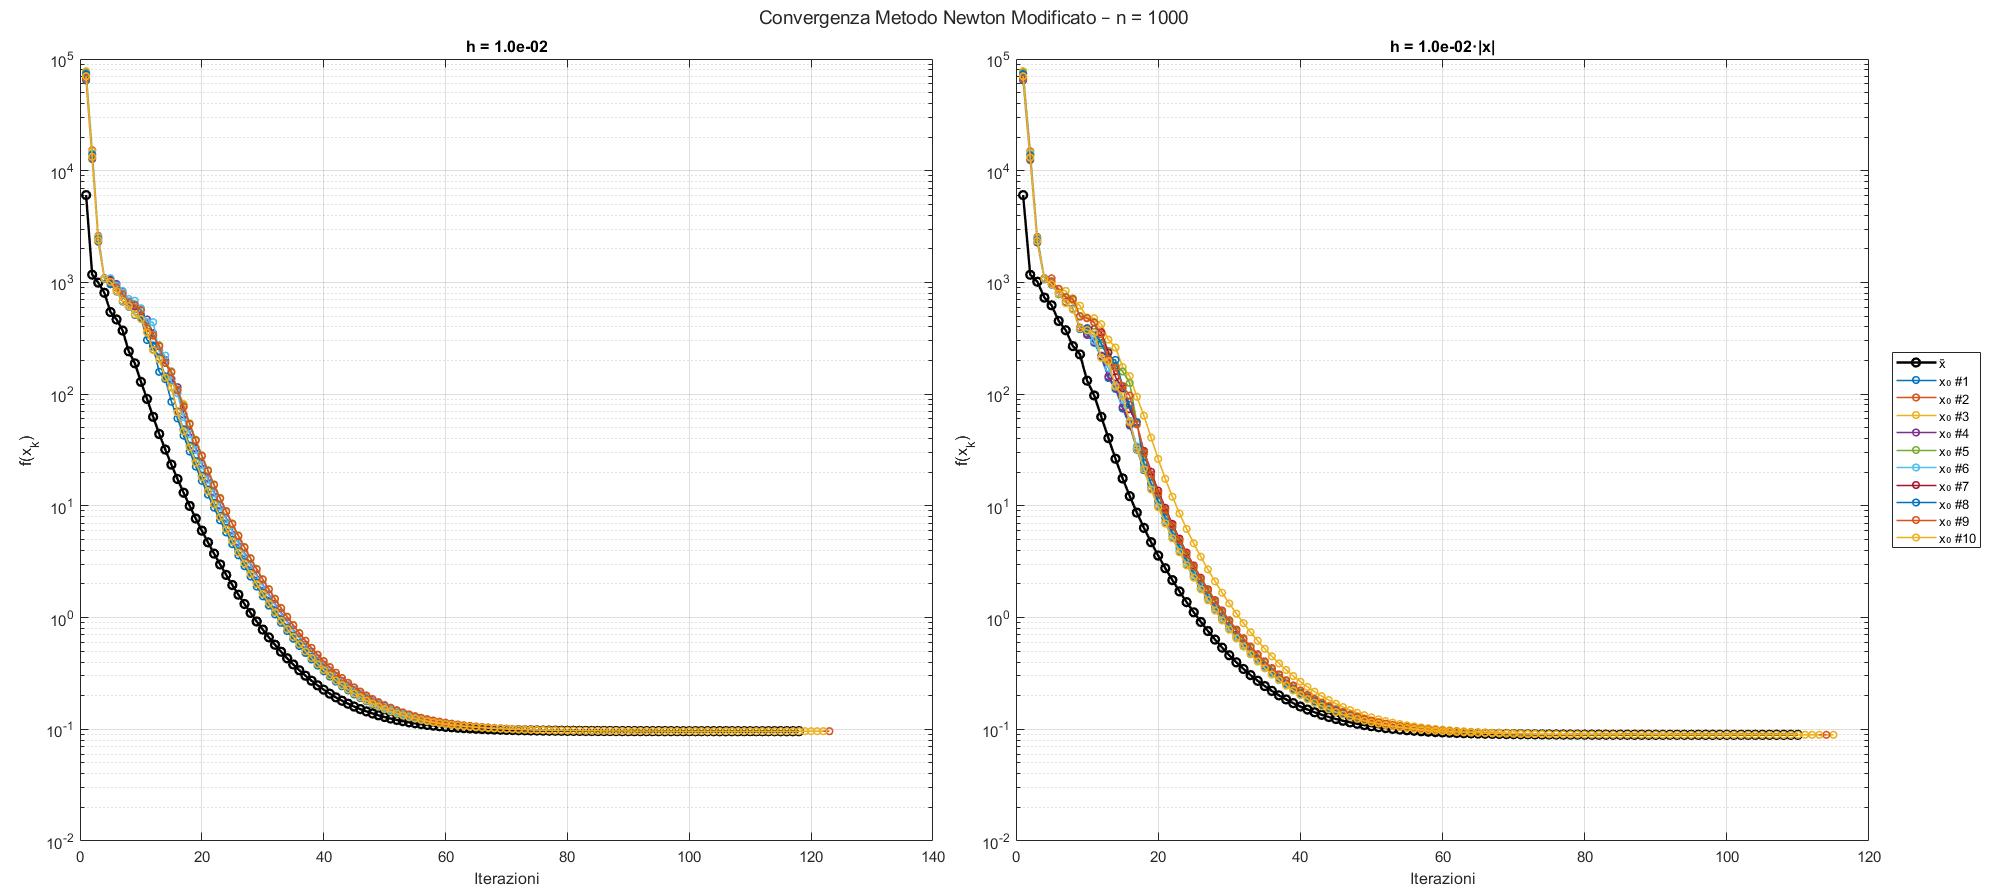
\includegraphics[width=\textwidth]{../immagini/ext_1k_h2.png}
			
			\endminipage\hfill
			\minipage{0.9\textwidth}
			\caption{Convergence of Modified Newton method on Extended Rosenbrock function in dimension $n = 10^{3}$ with fixed increment $h = 10^{-12}$ (left) and scaled increment $h = 10^{-12}\cdot|x|$ (right).}\label{fig:fd_1k_h12}
			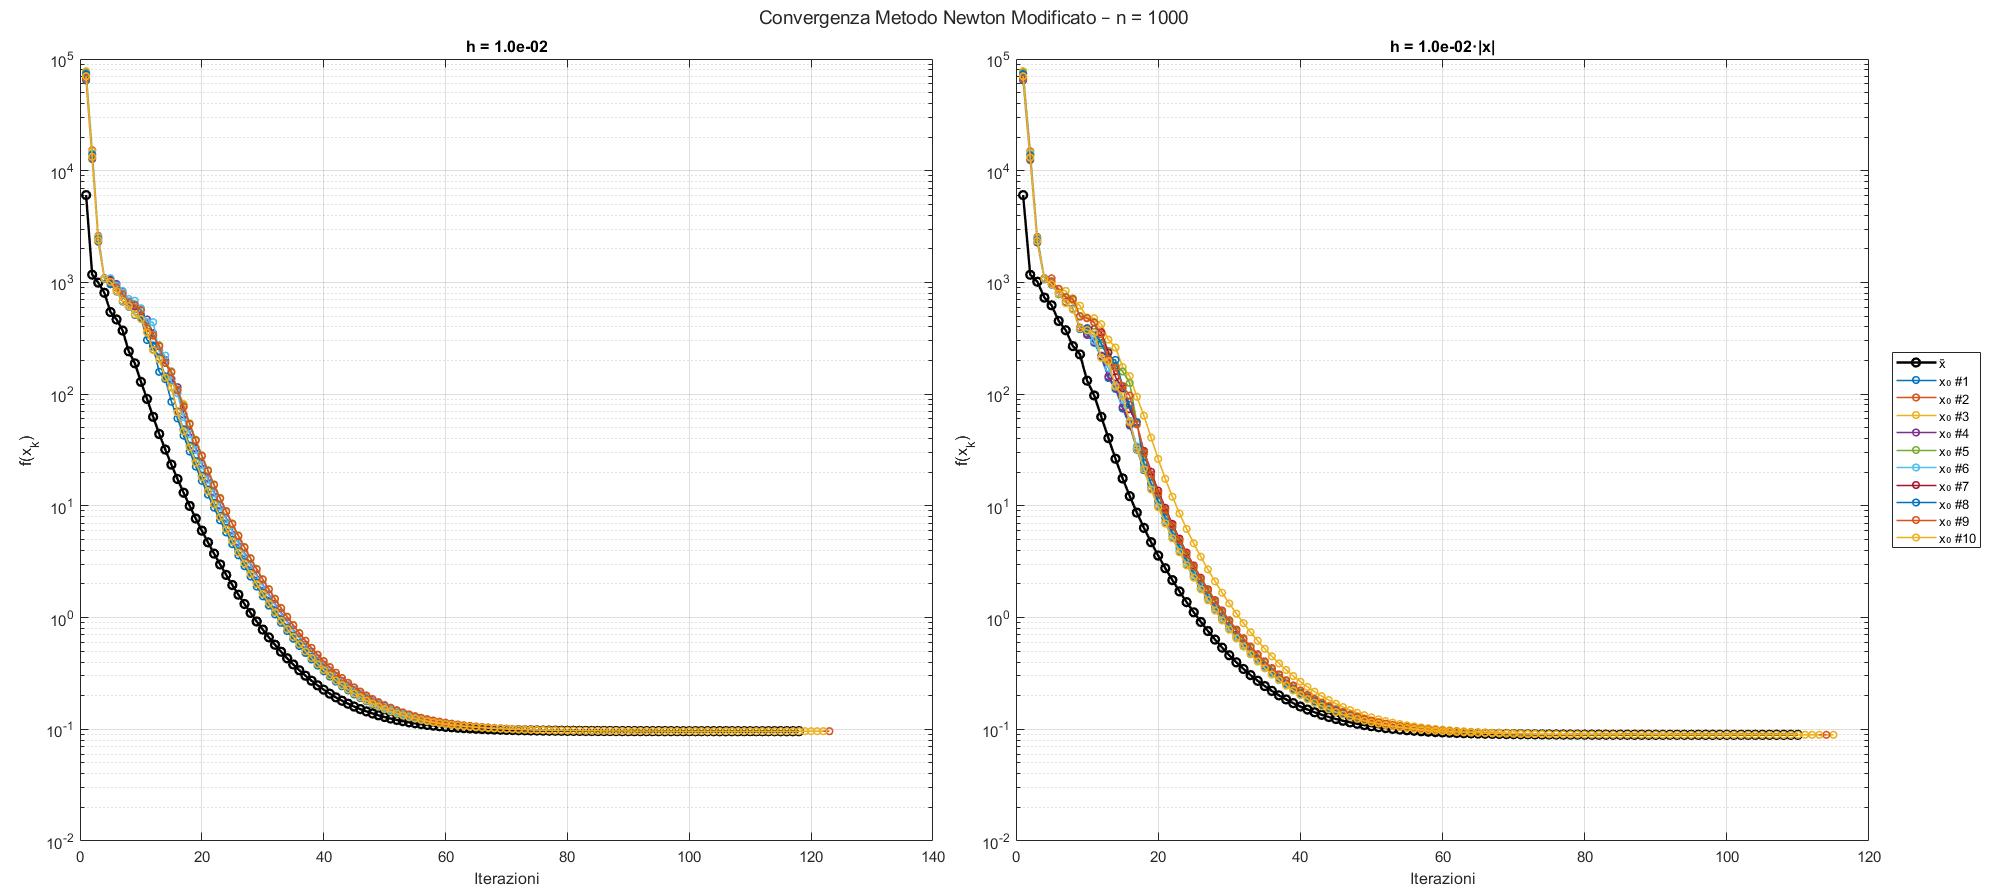
\includegraphics[width=\textwidth]{../immagini/ext_1k_h2.png}
			
			\endminipage\hfill
		\end{figure}
		
		
		%\begin{figure}[H]
		%	\centering
		%	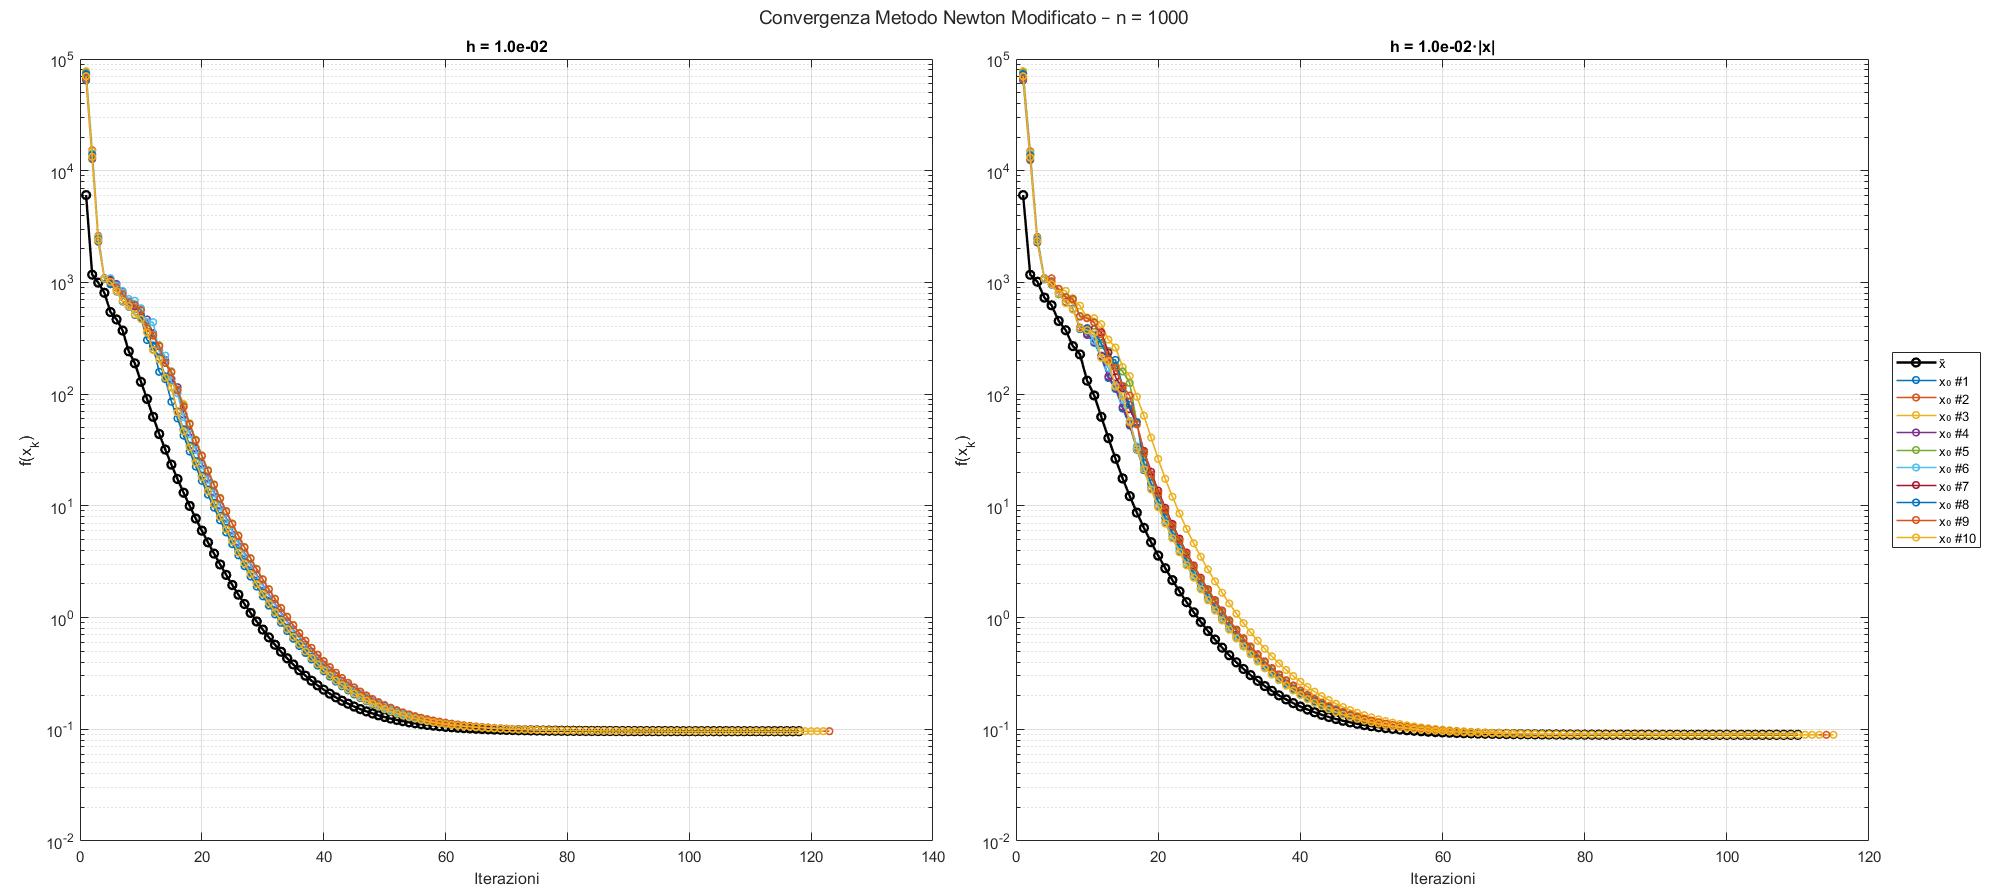
\includegraphics[width=\textwidth]{../immagini/ext_1k_h2.png}
		%	\caption{Convergence of Modified Newton method on Extended Rosenbrock function with fixed increment $h = 10^{-2}$ (left) and scaled increment $h = 10^{-2}\cdot|x|$ (right).}
		%	\label{fig:fd_1k_h2}
		%\end{figure}
		
		%\begin{figure}[htbp]
		%	\centering
		%	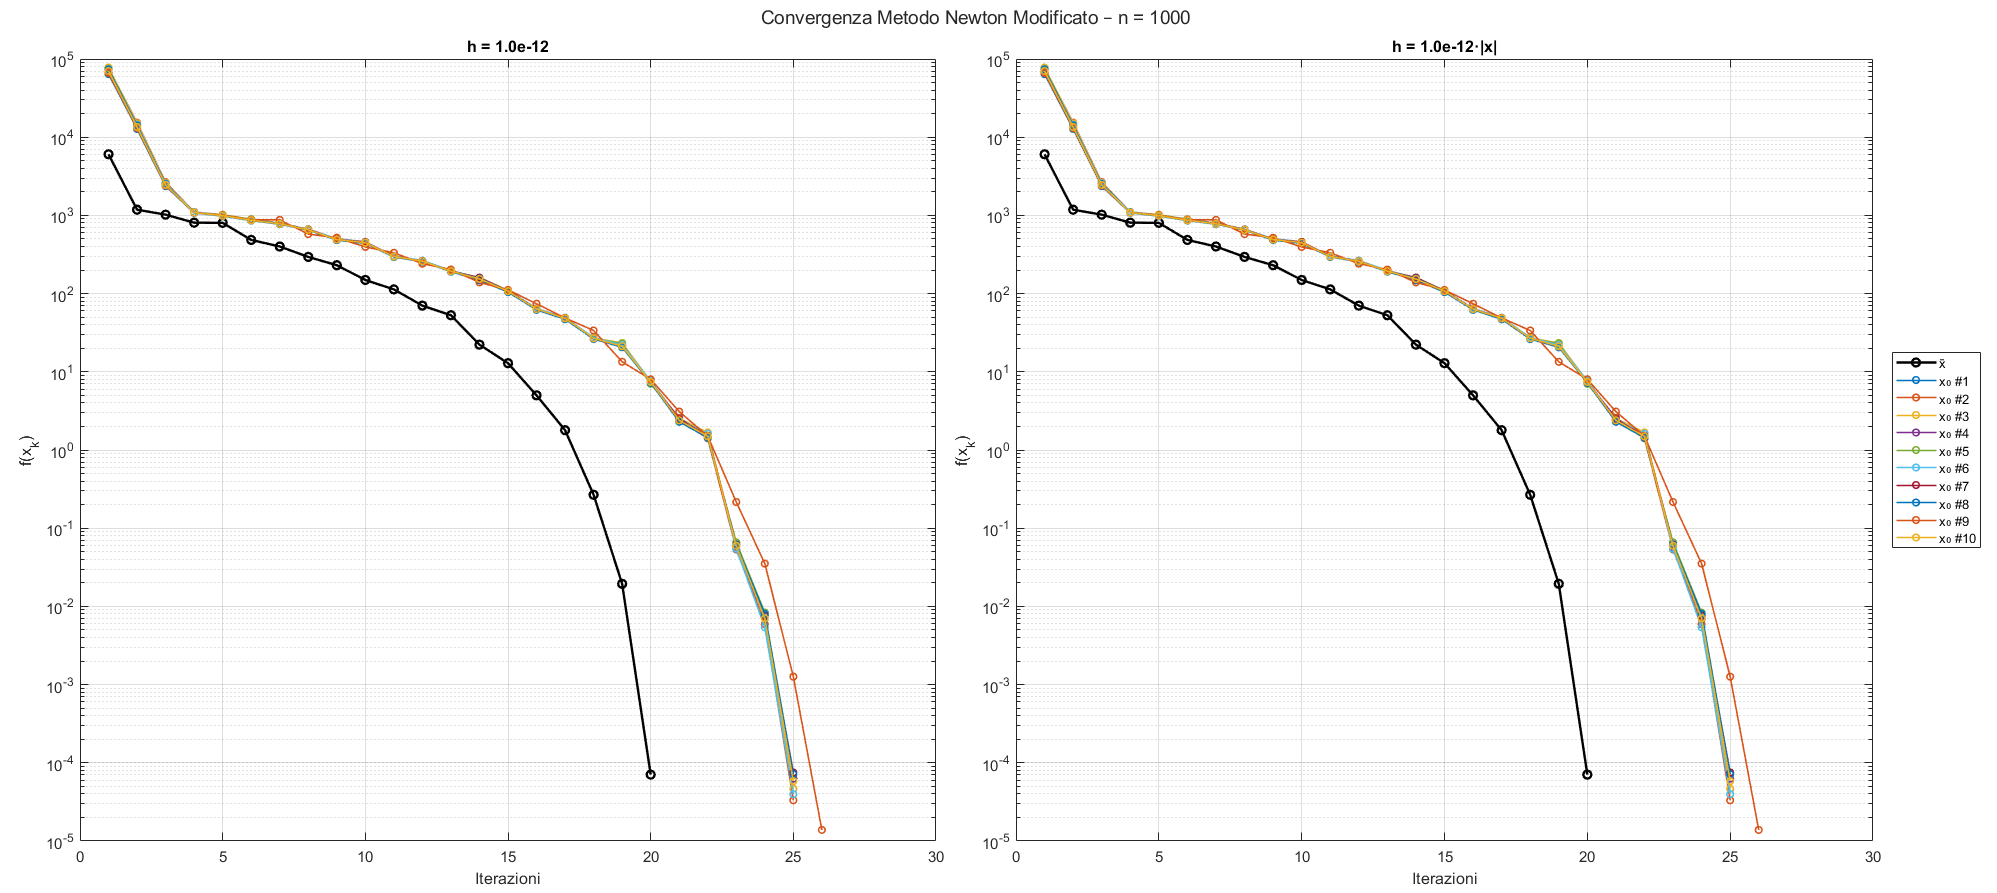
\includegraphics[width=\textwidth]{../immagini/ext_1k_h12.png}
		%	\caption{Convergence of Modified Newton method on Extended Rosenbrock function with fixed increment $h = 10^{-12}$ (left) and scaled increment $h = 10^{-12}\cdot|x|$ (right).}
		%	\label{fig:fd_1k_h12}
		%\end{figure}
		\newpage
		\item \boldmath $n = 10\,000$ \unboldmath
		
		\begin{table}[H]
			\centering
			\renewcommand{\arraystretch}{1.2}
			\resizebox{\textwidth}{!}{%
				\begin{tabular}{|c|c|c|c|c|c|}
					\hline
					\textbf{Increment} & \textbf{Init.} & \textbf{Iter} & \textbf{Time (s)} & \textbf{$\rho$} & \textbf{Successes} \\
					\hline
					$10^{-2}$ & $\bar{x}$ & 118 & 0.23 & 0.8856 & 0/10 \\
					$10^{-2}$ & Avg (10 pts) & 125.3 & 2.66 & 0.8856 & 0/10 \\
					$10^{-2}\cdot|x|$ & $\bar{x}$ & 110 & 0.21 & 0.8794 & 0/10 \\
					$10^{-2}\cdot|x|$ & Avg (10 pts) & 114.3 & 2.44 & 0.8794 & 0/10 \\
					\hline
					$10^{-4}$ & $\bar{x}$ & 21 & 0.04 & 1.1640 & 10/10 \\
					$10^{-4}$ & Avg (10 pts) & 27.0 & 0.92 & 1.2708 & 10/10 \\
					$10^{-4}\cdot|x|$ & $\bar{x}$ & 21 & 0.04 & 1.1476 & 10/10 \\
					$10^{-4}\cdot|x|$ & Avg (10 pts) & 27.0 & 0.91 & 1.2298 & 10/10 \\
					\hline
					$10^{-6}$ & $\bar{x}$ & 20 & 0.04 & 2.4144 & 10/10 \\
					$10^{-6}$ & Avg (10 pts) & 25.6 & 0.89 & 1.3572 & 10/10 \\
					$10^{-6}\cdot|x|$ & $\bar{x}$ & 20 & 0.04 & 2.4464 & 10/10 \\
					$10^{-6}\cdot|x|$ & Avg (10 pts) & 25.6 & 0.89 & 1.3581 & 10/10 \\
					\hline
					$10^{-8}$ & $\bar{x}$ & 20 & 0.04 & 2.1463 & 10/10 \\
					$10^{-8}$ & Avg (10 pts) & 25.6 & 0.90 & 1.3626 & 10/10 \\
					$10^{-8}\cdot|x|$ & $\bar{x}$ & 20 & 0.04 & 2.1468 & 10/10 \\
					$10^{-8}\cdot|x|$ & Avg (10 pts) & 25.6 & 0.90 & 1.3626 & 10/10 \\
					\hline
					$10^{-10}$ & $\bar{x}$ & 20 & 0.04 & 2.1432 & 10/10 \\
					$10^{-10}$ & Avg (10 pts) & 25.6 & 0.90 & 1.3626 & 10/10 \\
					$10^{-10}\cdot|x|$ & $\bar{x}$ & 20 & 0.04 & 2.1432 & 10/10 \\
					$10^{-10}\cdot|x|$ & Avg (10 pts) & 25.6 & 0.90 & 1.3626 & 10/10 \\
					\hline
					$10^{-12}$ & $\bar{x}$ & 20 & 0.04 & 2.1432 & 10/10 \\
					$10^{-12}$ & Avg (10 pts) & 25.6 & 0.90 & 1.3626 & 10/10 \\
					$10^{-12}\cdot|x|$ & $\bar{x}$ & 20 & 0.04 & 2.1432 & 10/10 \\
					$10^{-12}\cdot|x|$ & Avg (10 pts) & 25.6 & 0.90 & 1.3626 & 10/10 \\
					\hline
				\end{tabular}%
			}
			\caption{Finite difference results for using different typology of increments ($n = 10^{4}$).}
			\label{tab:fd_er_10000}
		\end{table}
		
		\newpage
		
		\begin{figure}[H]%[!htb]
			\minipage{0.9\textwidth}
			\caption{Convergence of Modified Newton method on Extended Rosenbrock function in dimension $n = 10^{4}$ with fixed increment $h = 10^{-2}$ (left) and scaled increment $h = 10^{-2}\cdot|x|$ (right).}\label{fig:fd_10k_h2}
			
			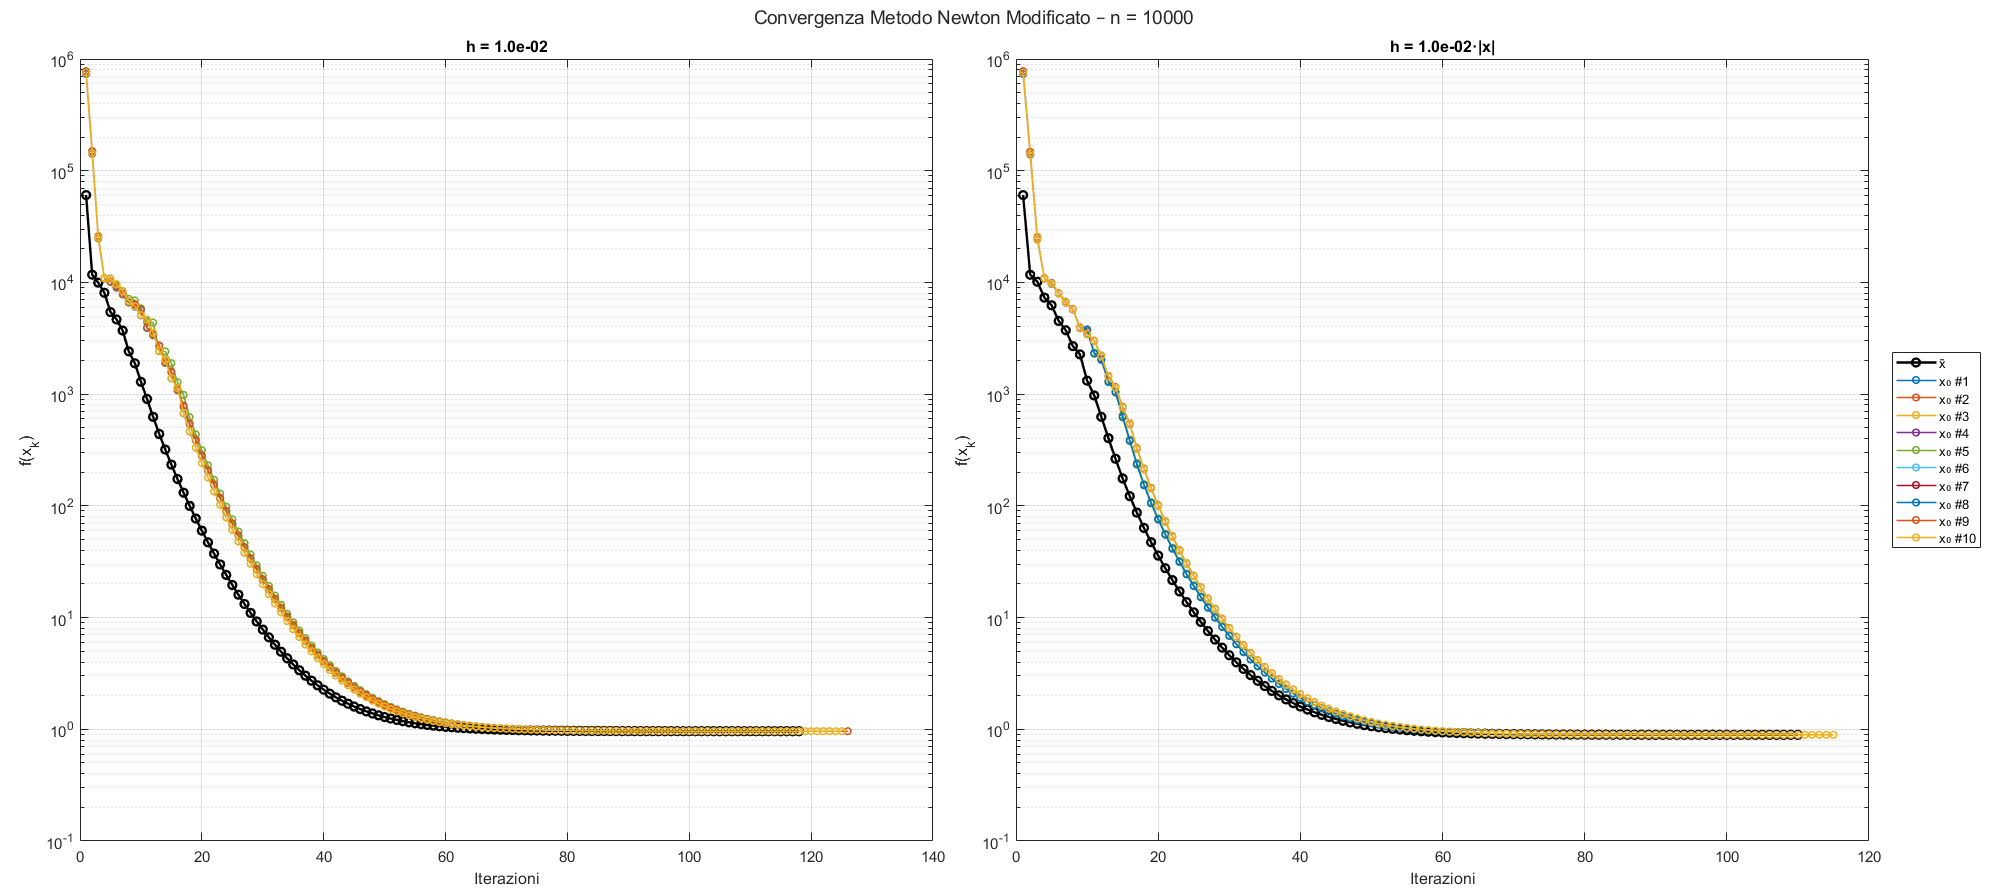
\includegraphics[width=\textwidth]{../immagini/ext_10k_h2.png}
			\endminipage\hfill
			\minipage{0.9\textwidth}
			\caption{Convergence of Modified Newton method on Extended Rosenbrock function in dimension $n = 10^{4}$ with fixed increment $h = 10^{-12}$ (left) and scaled increment $h = 10^{-12}\cdot|x|$ (right).} 			\label{fig:fd_10k_h12}	
			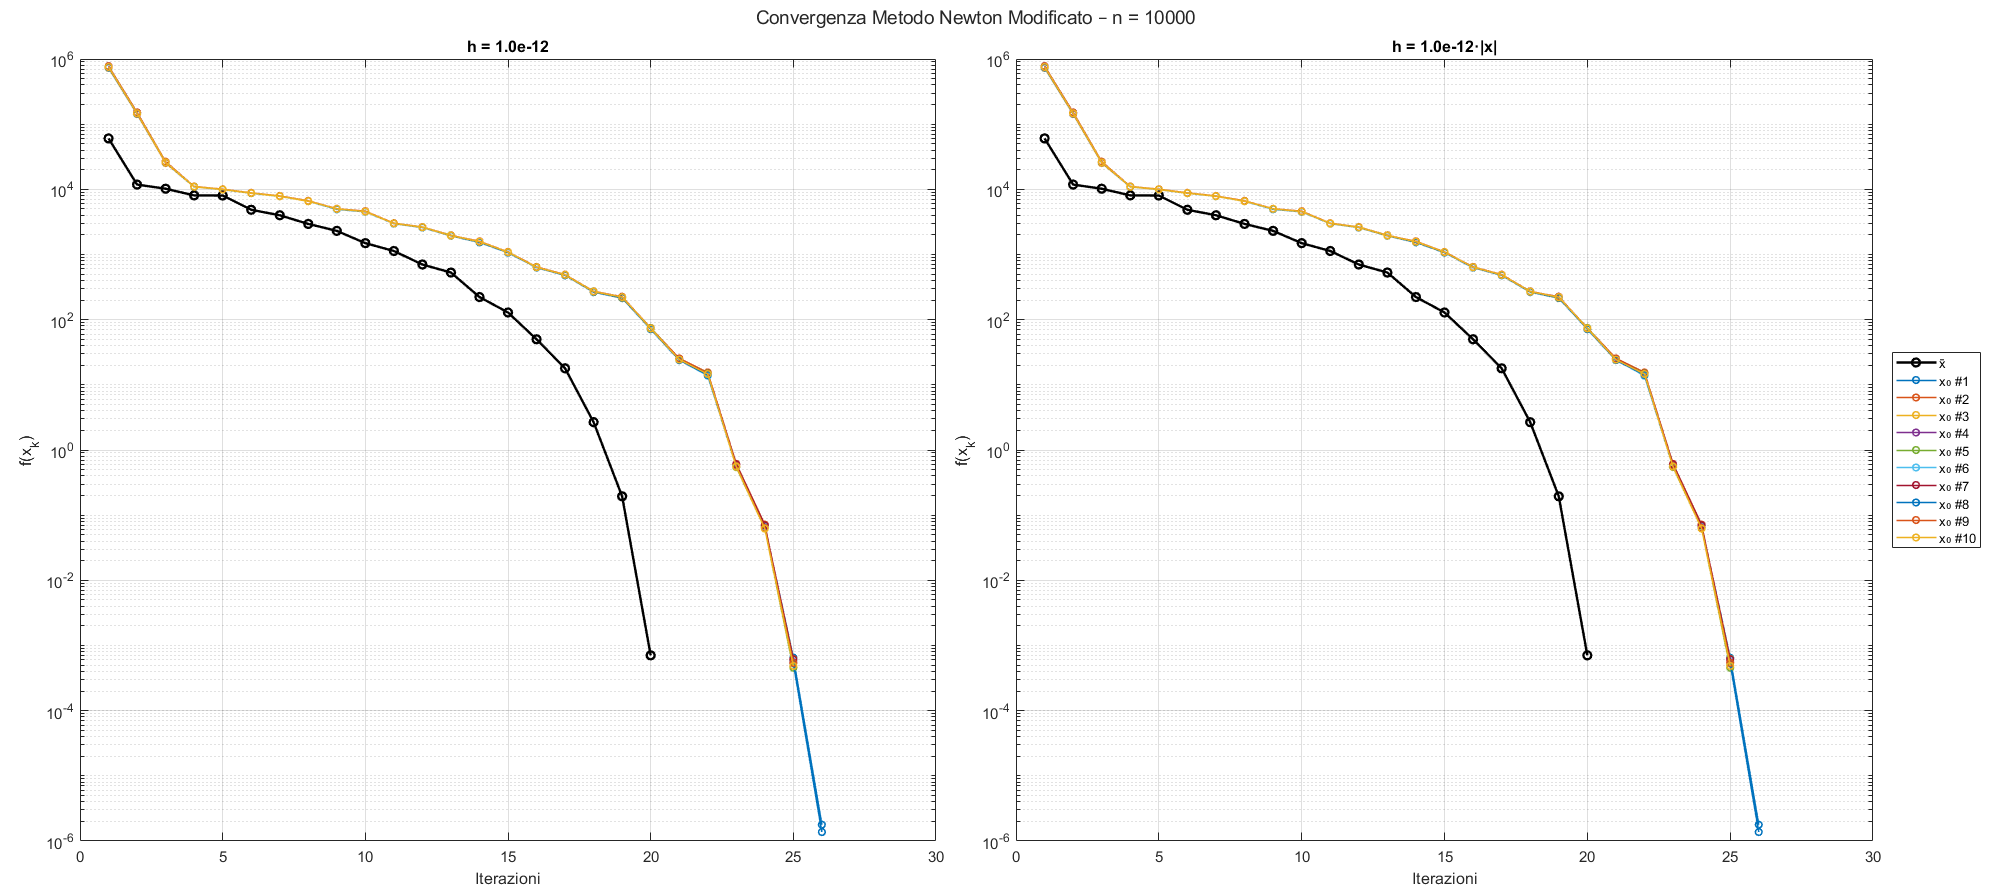
\includegraphics[width=\textwidth]{../immagini/ext_10k_h12.png}
		
			\endminipage\hfill
		\end{figure}
		
		
		
		
		%\begin{figure}[H]
		%	\centering
		%	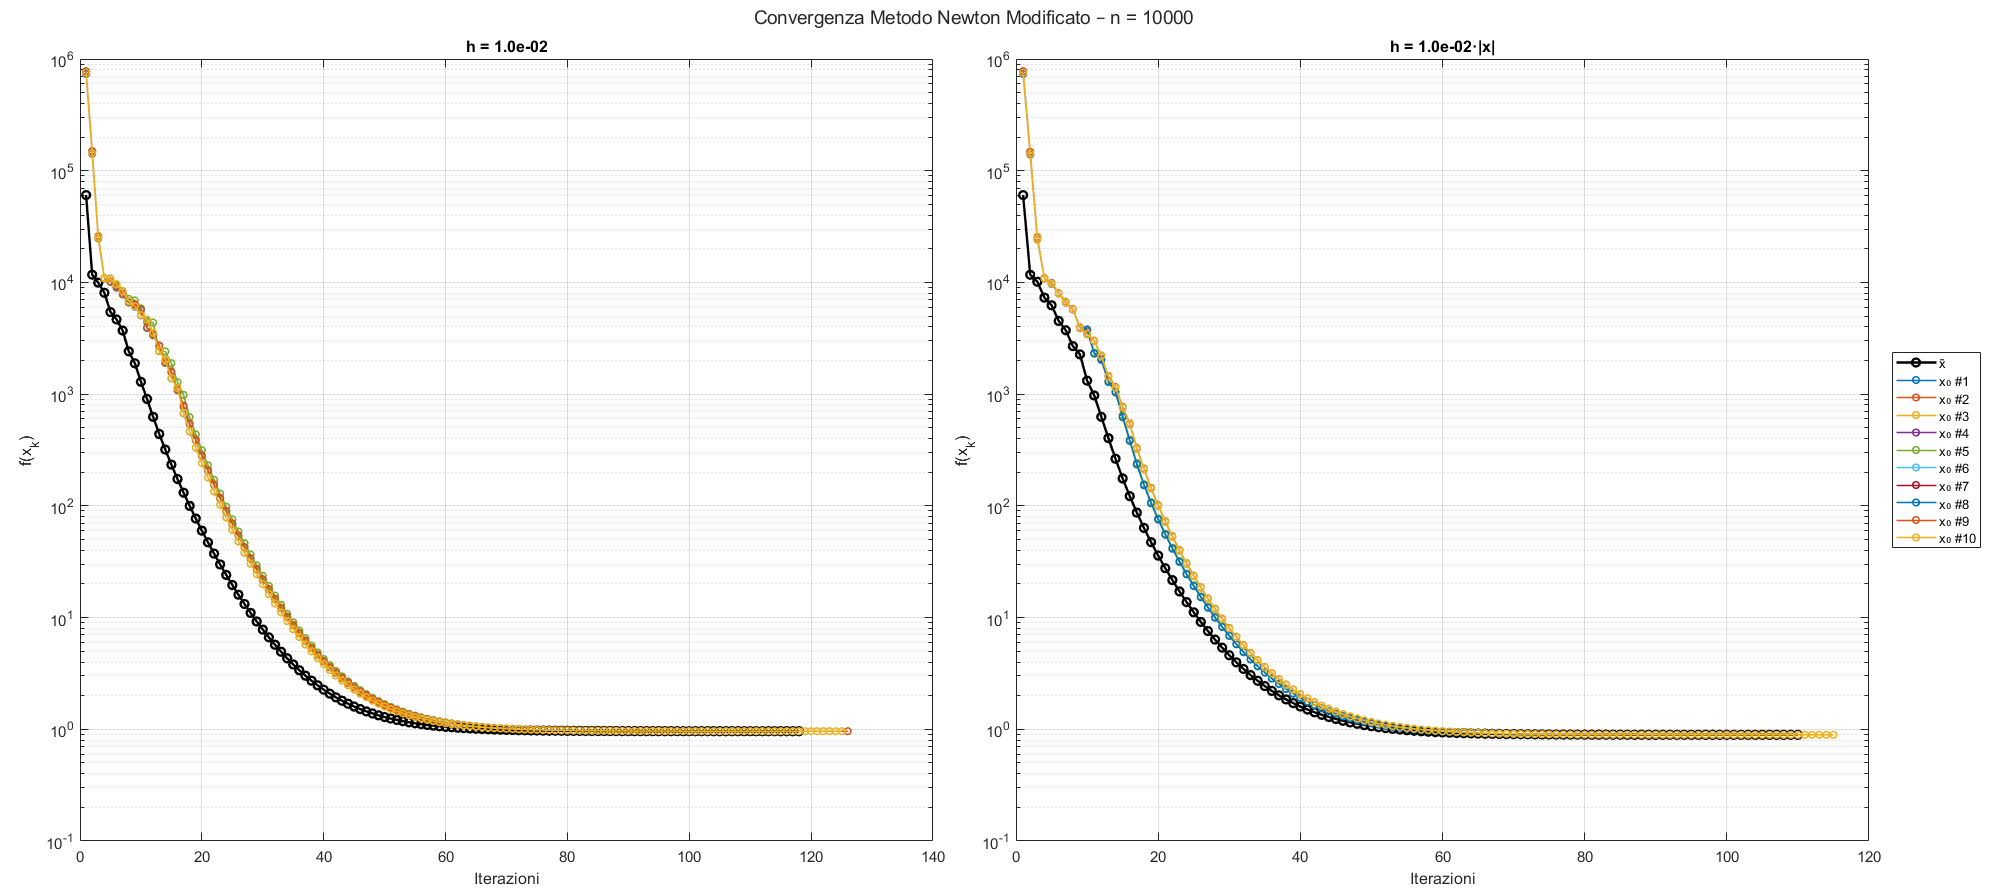
\includegraphics[width=\textwidth]{../immagini/ext_10k_h2.png}
		%	\caption{Convergence of Modified Newton method on Extended Rosenbrock function in dimension $n = 10^{4}$ with fixed increment $h = 10^{-2}$ (left) and scaled increment $h = 10^{-2}\cdot|x|$ (right).}
		%	\label{fig:fd_10k_h2}
		%\end{figure}
		
%		\begin{figure}[htbp]
%			\centering
%			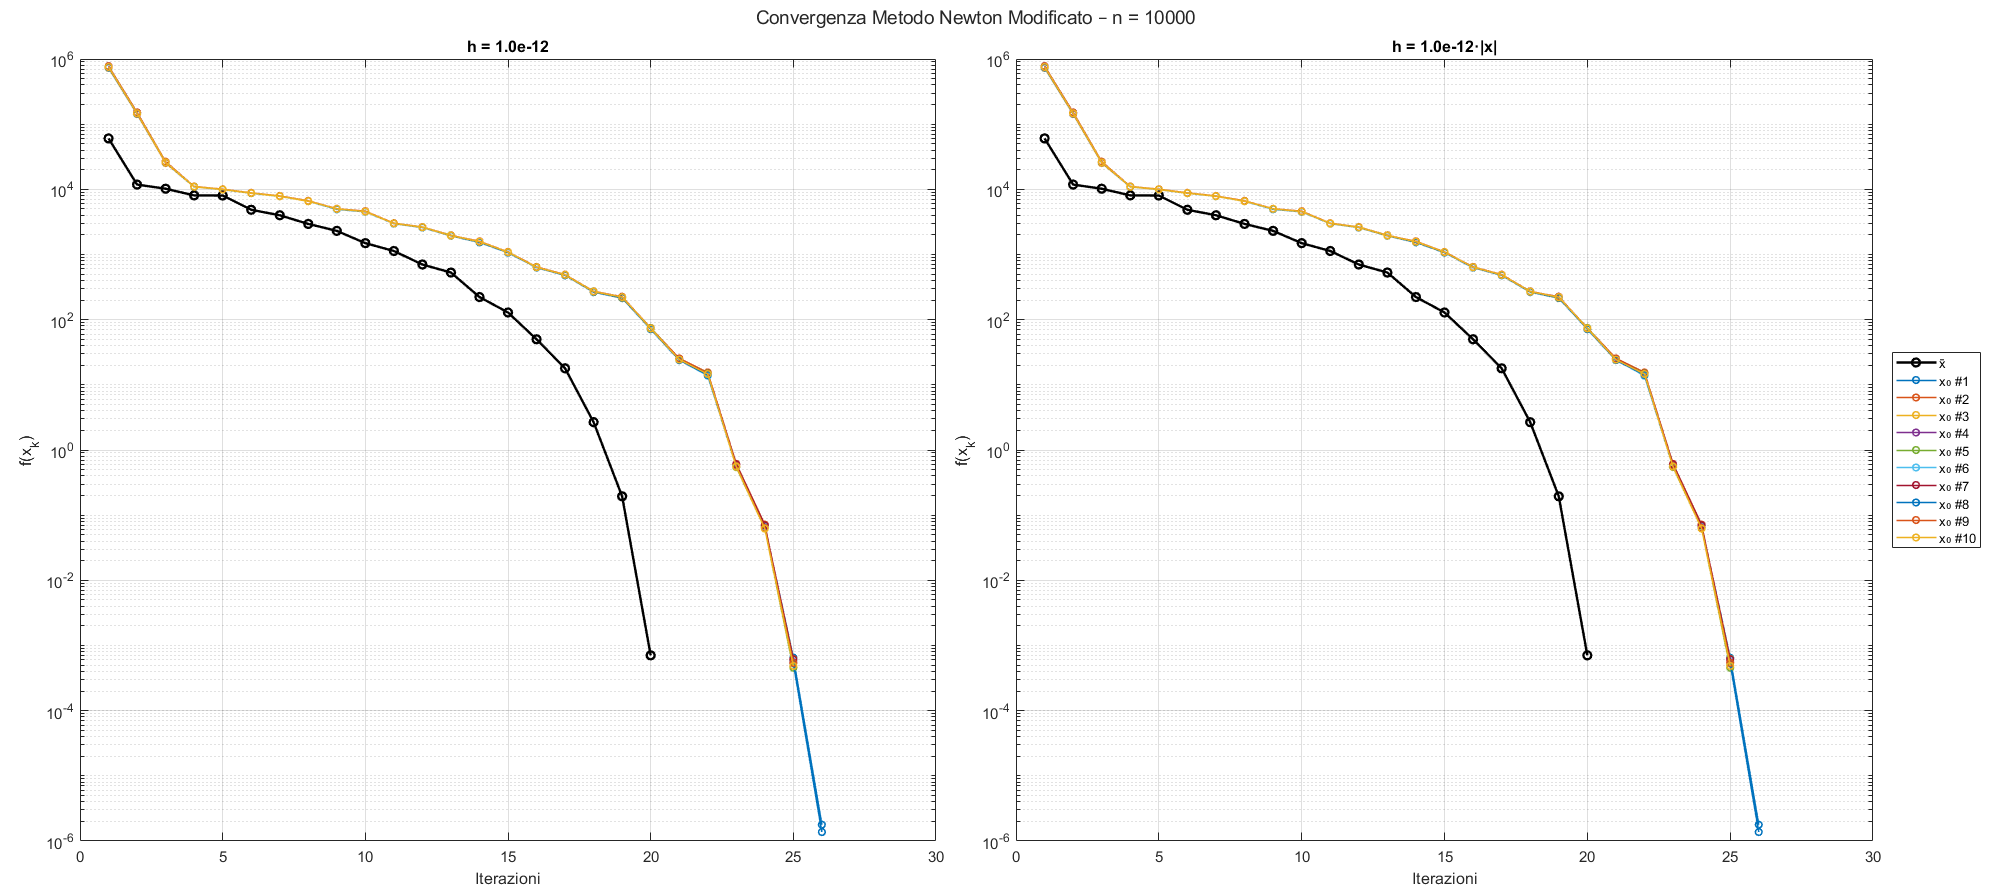
\includegraphics[width=\textwidth]{../immagini/ext_10k_h12.png}
%			\caption{Convergence of Modified Newton method on Extended Rosenbrock function in dimension $n = 10^{4}$ with fixed increment $h = 10^{-12}$ (left) and scaled increment $h = 10^{-12}\cdot|x|$ (right).}
%			\label{fig:fd_10k_h12}
%		\end{figure}
		
		
		
			%\vspace{1em}
		%\vspace{1em}
		
		
		\newpage
		\item \boldmath $n = 100\,000$ \unboldmath
		
		\vspace{1em}
		
		\begin{table}[H]
			\centering
			\renewcommand{\arraystretch}{1.2}
			\resizebox{\textwidth}{!}{%
				\begin{tabular}{|c|c|c|c|c|c|}
					\hline
					\textbf{Increment} & \textbf{Init.} & \textbf{Iter} & \textbf{Time (s)} & \textbf{$\rho$} & \textbf{Successes} \\
					\hline
					$10^{-2}$ & $\bar{x}$ & 118 & 2.66 & 0.8856 & 0/10 \\
					$10^{-2}$ & Avg (10 pts) & 126.0 & 3.26 & 0.8856 & 0/10 \\
					$10^{-2}\cdot|x|$ & $\bar{x}$ & 110 & 2.41 & 0.8794 & 0/10 \\
					$10^{-2}\cdot|x|$ & Avg (10 pts) & 114.2 & 2.94 & 0.8794 & 0/10 \\
					\hline
					$10^{-4}$ & $\bar{x}$ & 22 & 0.49 & 0.9324 & 10/10 \\
					$10^{-4}$ & Avg (10 pts) & 27.0 & 0.92 & 1.2738 & 10/10 \\
					$10^{-4}\cdot|x|$ & $\bar{x}$ & 22 & 0.49 & 0.9453 & 10/10 \\
					$10^{-4}\cdot|x|$ & Avg (10 pts) & 27.0 & 0.91 & 1.2309 & 10/10 \\
					\hline
					$10^{-6}$ & $\bar{x}$ & 20 & 0.44 & 2.4144 & 10/10 \\
					$10^{-6}$ & Avg (10 pts) & 26.0 & 0.89 & 1.3622 & 10/10 \\
					$10^{-6}\cdot|x|$ & $\bar{x}$ & 20 & 0.44 & 2.4464 & 10/10 \\
					$10^{-6}\cdot|x|$ & Avg (10 pts) & 26.0 & 0.89 & 1.3620 & 10/10 \\
					\hline
					$10^{-8}$ & $\bar{x}$ & 20 & 0.44 & 2.1463 & 10/10 \\
					$10^{-8}$ & Avg (10 pts) & 26.0 & 0.90 & 1.3633 & 10/10 \\
					$10^{-8}\cdot|x|$ & $\bar{x}$ & 20 & 0.44 & 2.1468 & 10/10 \\
					$10^{-8}\cdot|x|$ & Avg (10 pts) & 26.0 & 0.90 & 1.3633 & 10/10 \\
					\hline
					$10^{-10}$ & $\bar{x}$ & 20 & 0.45 & 2.1432 & 10/10 \\
					$10^{-10}$ & Avg (10 pts) & 26.0 & 0.90 & 1.3632 & 10/10 \\
					$10^{-10}\cdot|x|$ & $\bar{x}$ & 20 & 0.44 & 2.1432 & 10/10 \\
					$10^{-10}\cdot|x|$ & Avg (10 pts) & 26.0 & 0.90 & 1.3632 & 10/10 \\
					\hline
					$10^{-12}$ & $\bar{x}$ & 20 & 0.44 & 2.1432 & 10/10 \\
					$10^{-12}$ & Avg (10 pts) & 26.0 & 0.89 & 1.3632 & 10/10 \\
					$10^{-12}\cdot|x|$ & $\bar{x}$ & 20 & 0.44 & 2.1432 & 10/10 \\
					$10^{-12}\cdot|x|$ & Avg (10 pts) & 26.0 & 0.89 & 1.3632 & 10/10 \\
					\hline
				\end{tabular}%
			}
			\label{tab:fd_rosenbrock_100000}
			\caption{Finite difference results using different increments ($n = 10^{5}$).}
		\end{table}
		
		\newpage
		
		\begin{figure}[H]%[!htb]
			\minipage{0.9\textwidth}
			\caption{Convergence of Modified Newton method on Extended Rosenbrock function ($n = 10^{5}$) with fixed increment $h = 10^{-2}$ (left) and scaled increment $h = 10^{-2}\cdot|x|$ (right).}
			\label{fig:fd_100k_h2}			
			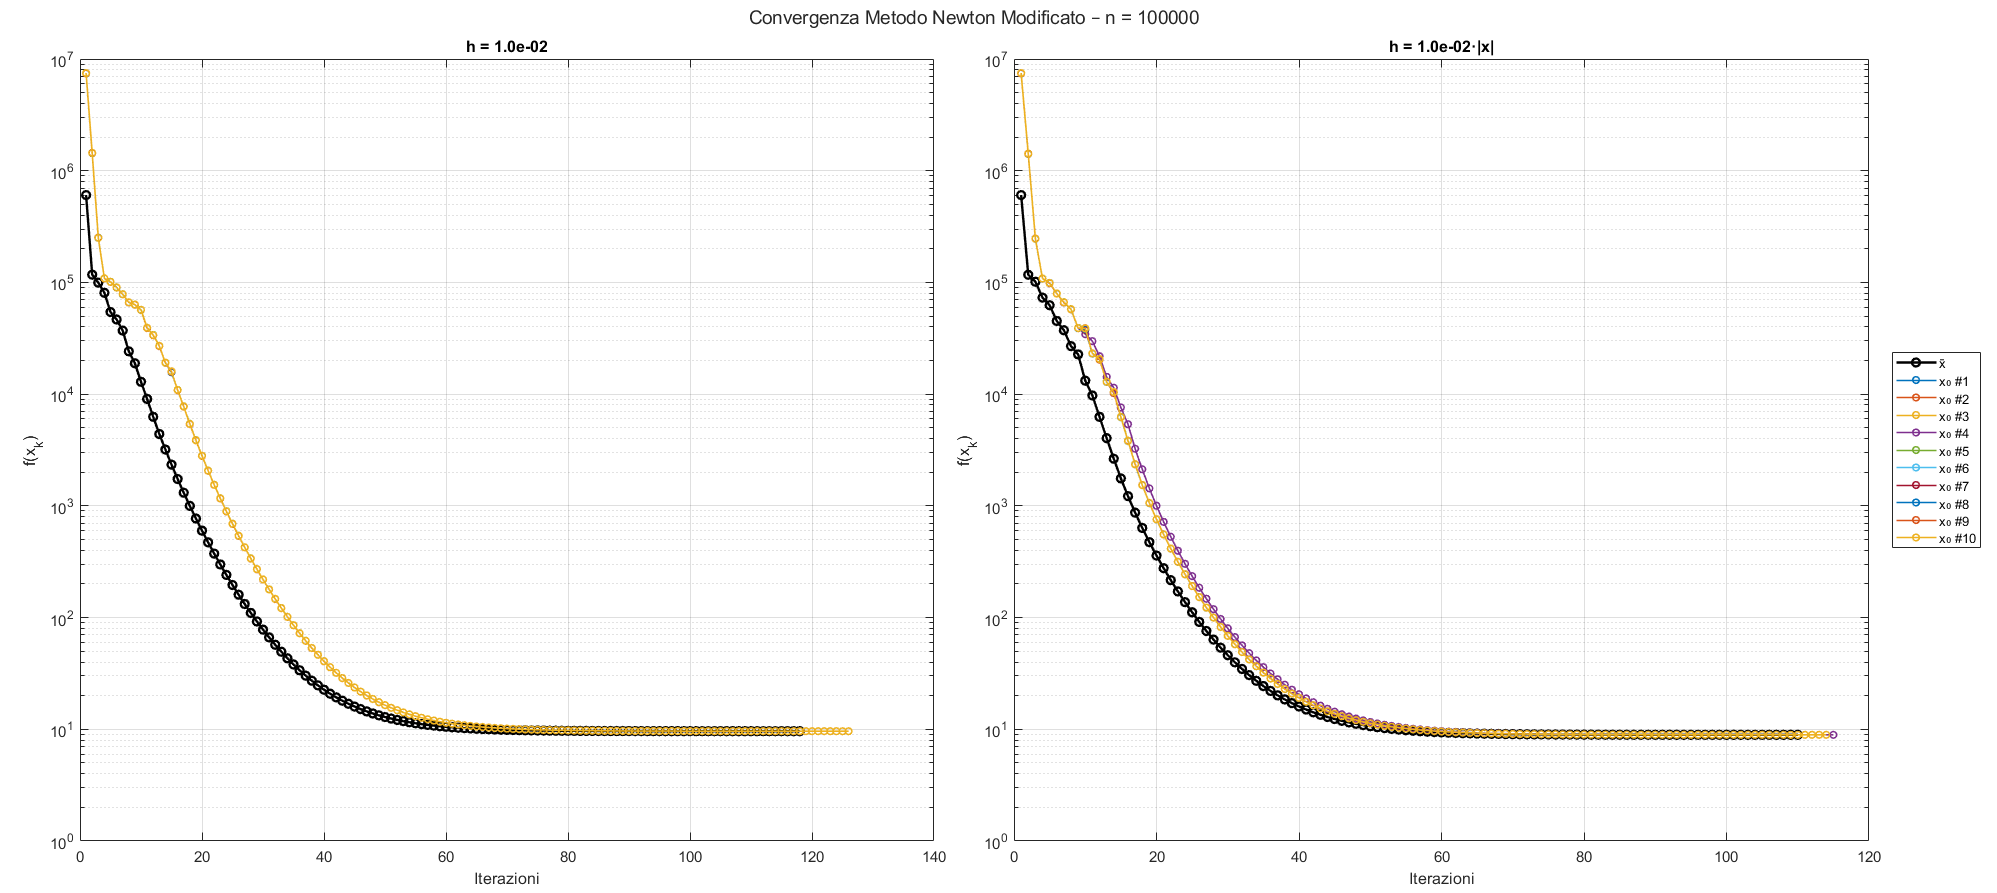
\includegraphics[width=\textwidth]{../immagini/ext_100k_h2.png}
			\endminipage\hfill
			\minipage{0.9\textwidth}
			\caption{Convergence of Modified Newton method on Extended Rosenbrock function ($n = 10^{5}$) with fixed increment $h = 10^{-12}$ (left) and scaled increment $h = 10^{-12}\cdot|x|$ (right).}
			\label{fig:fd_100k_h12}
			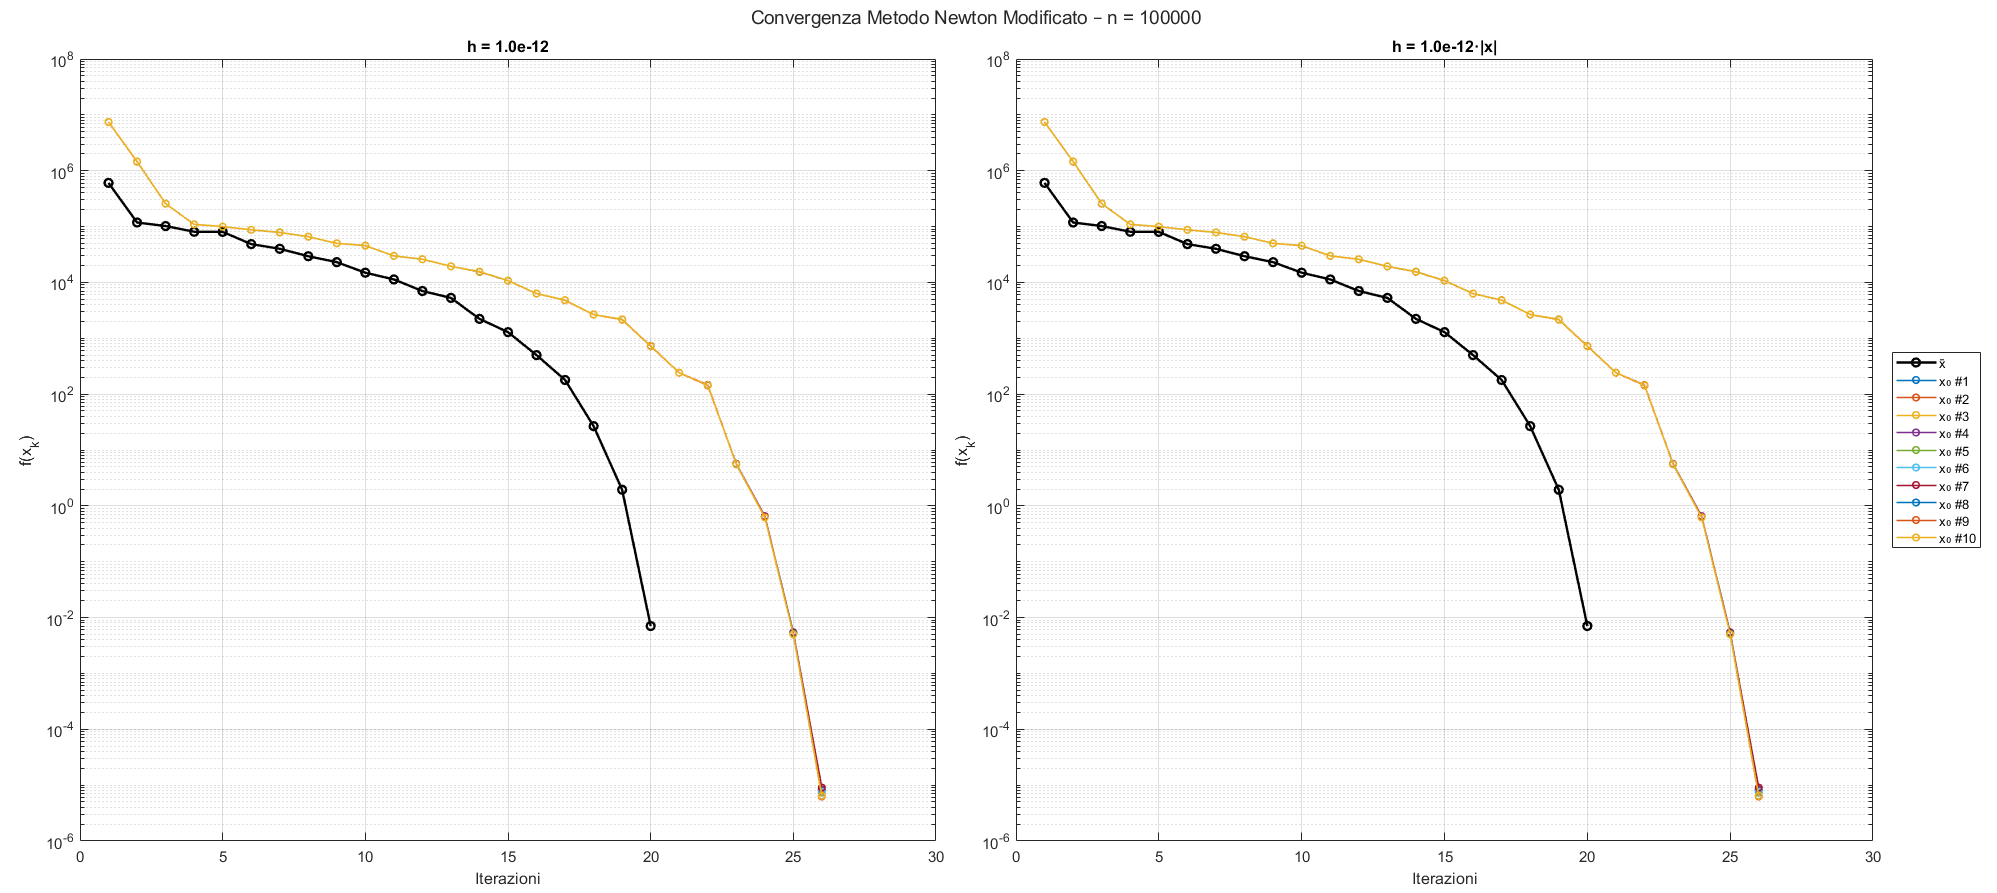
\includegraphics[width=\textwidth]{../immagini/ext_100k_h12.png}
			\endminipage\hfill
		\end{figure}
		
		
		
		
		
		%\begin{figure}[H]
		%	\centering
		%	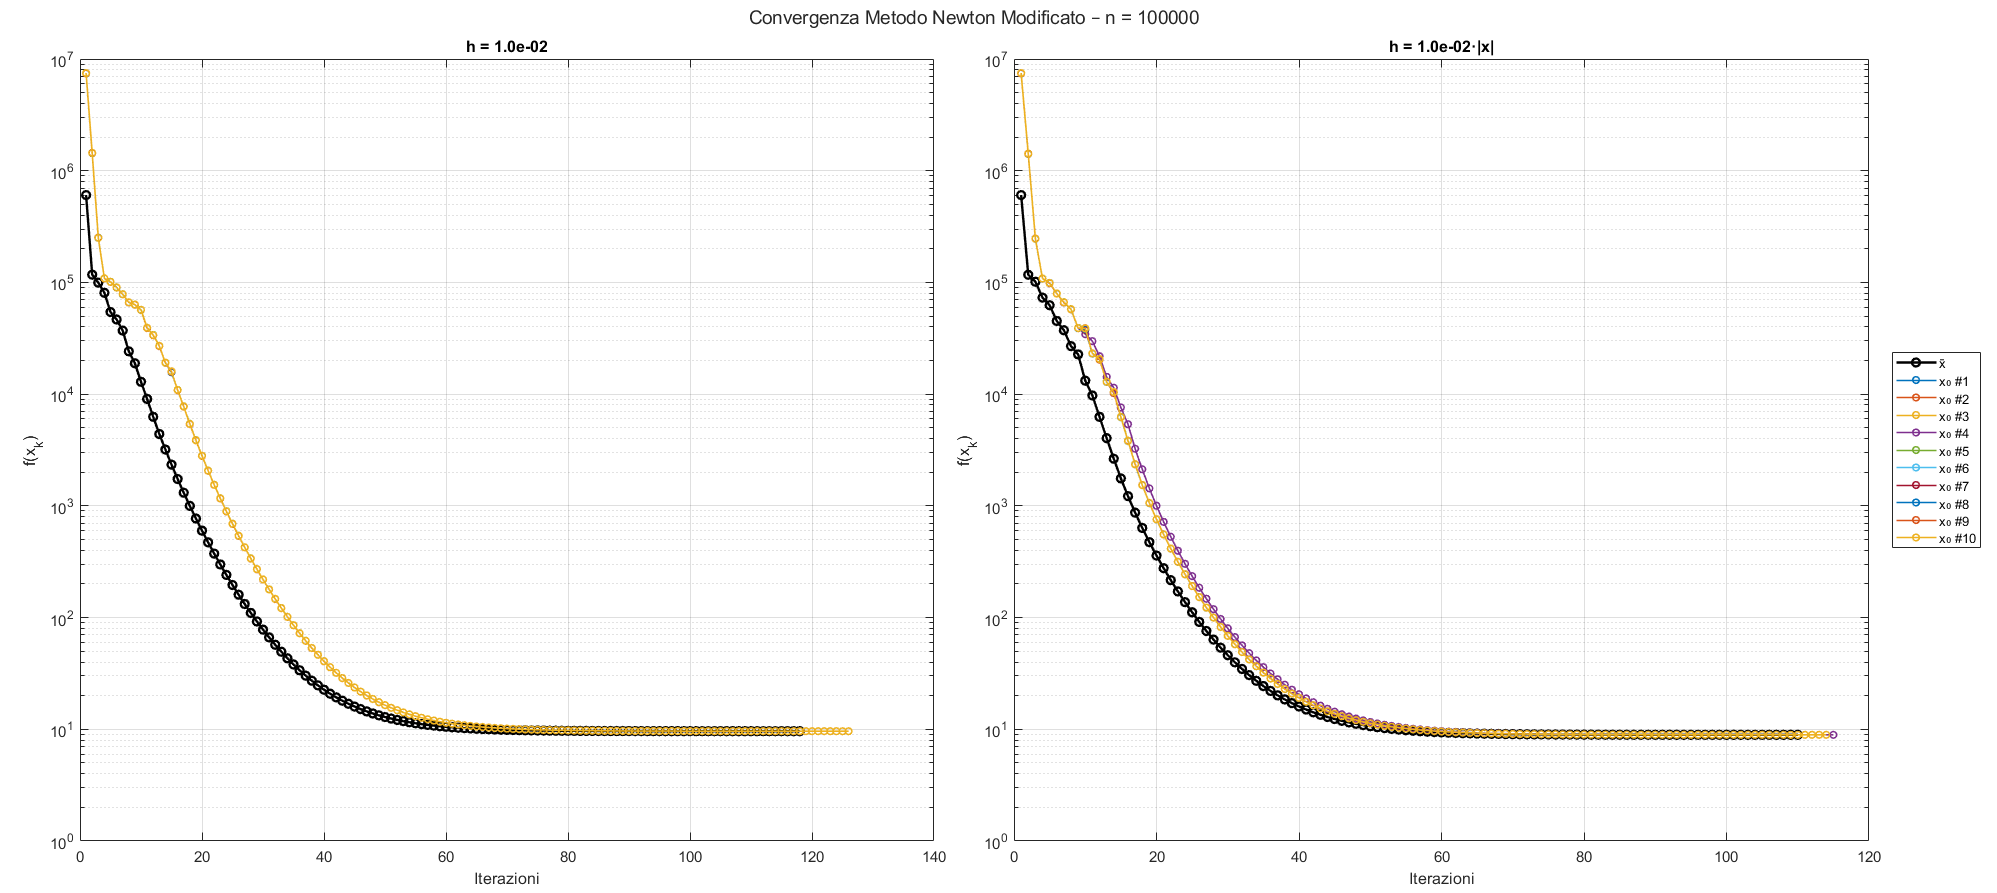
\includegraphics[width=\textwidth]{../immagini/ext_100k_h2.png}
		%	\caption{Convergence of Modified Newton method on Extended Rosenbrock function ($n=100\,000$) with fixed increment $h = 10^{-2}$ (left) and scaled increment $h = 10^{-2}\cdot|x|$ (right).}
		%	\label{fig:fd_100k_h2}
		%\end{figure}
		
		%\begin{figure}[htbp]
		%	\centering
		%	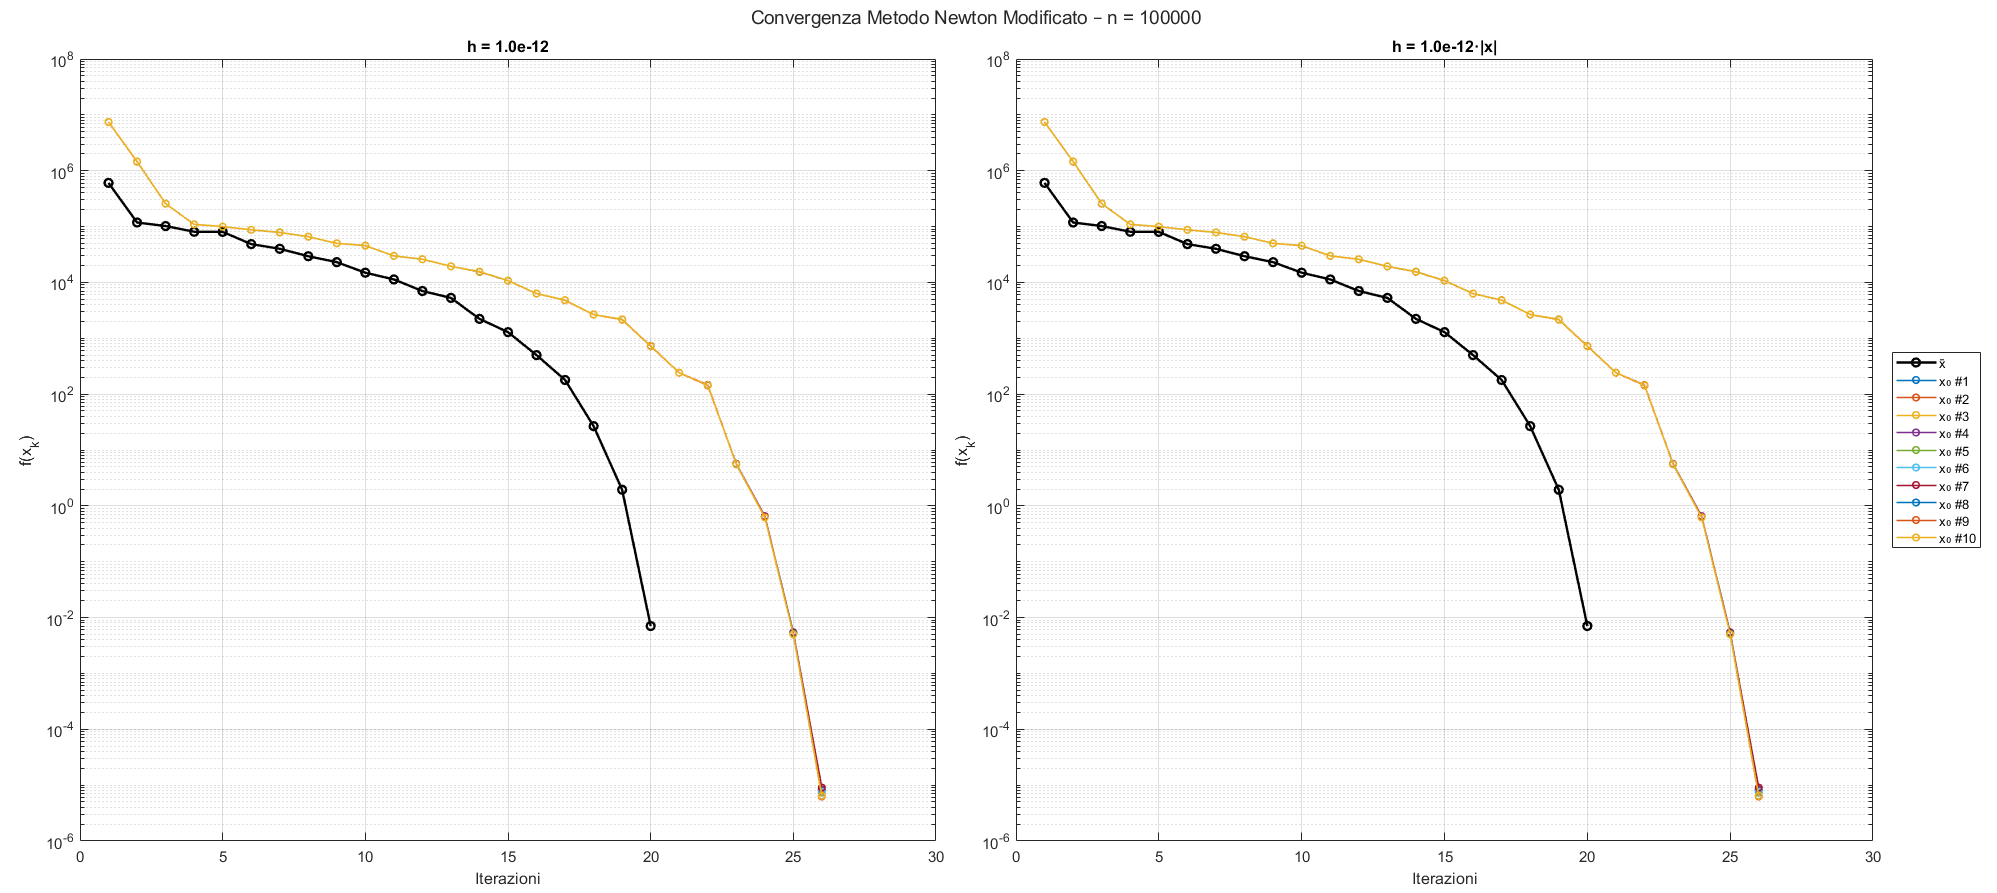
\includegraphics[width=\textwidth]{../immagini/ext_100k_h12.png}
		%	\caption{Convergence of Modified Newton method on Extended Rosenbrock function ($n=100\,000$) with fixed increment $h = 10^{-12}$ (left) and scaled increment $h = 10^{-12}\cdot|x|$ (right).}
		%	\label{fig:fd_100k_h12}
		%\end{figure}
		
		\end{itemize}
	
	\newpage
	\subsection{Nelder–Mead method}
	In this subsection are shown the results obtained from the minimization of the Extended Rosenbrock function using the Nelder--Mead method. Before presenting the results, a general experimental setup is given:
	\begin{itemize}
		\item \texttt{n} $= 10, 26, 50$;
		\item \texttt{max\_iter} $= 80.000$;
		\item \texttt{tol} $= 10^{-6}$.
	\end{itemize}
	%	\vspace{0.5cm}
	
	Moreover, for each run were recorded:
	\begin{itemize}
		\item number of iterations to convergence;
		\item CPU time;
		\item final objective value found \(f_{min}\);
		\item experimental rate of convergence \(\rho\):
		\[
		\rho \approx \frac{\log\left(\|x^{(k+1)} - x^{(k)}\|\big/\|x^{(k)} - x^{(k-1)}\|\right)}{\log\left(\|x^{(k)} - x^{(k-1)}\|\big/\|x^{(k-1)} - x^{(k-2)}\|\right)}.
		\]
			\end{itemize}	
	
	In correspondence with the randomly generated points, an average behavior of each of the previous catogories is reported.
	\paragraph{Experimental results.}The algorithm successfully runs on all dimensions, but convergence was never achieved within tolerance. The number of iterations and function values clearly indicate that Nelder–Mead is not effective on this problem; incidentally, in all cases the final function values remained far from zero, indicating that Nelder–Mead struggled with this function even in low dimensions. The high curvature and narrow valleys of the Extended Rosenbrock function severely impact the simplex--based exploration. Furthermore, while runtime remains reasonable, the algorithm not only requires thousands of iterations to make progress but also does not reach values close to zero. This confirms the known limitations of Nelder–Mead in high--dimensional landscapes.
	
	
	\begin{table}[H]
		\renewcommand{\arraystretch}{1.2}
		\resizebox{\textwidth}{!}{%
			\begin{tabular}{|c|c|c|c|c|c|}
				\hline
				\textbf{Dimension} & \textbf{Starting point} & \textbf{$f_{\min}$} & \textbf{Iter} & \textbf{Time (s)} & \textbf{$\rho$} \\
				\hline
				10  & $\bar{x}$         & 4.755805   & 1807   & 0.04 & 0.9082  \\
				& Avg (10 pts)      & 8.248833   & 1221   & 0.016 & 0.0500 \\
				\hline
				26  & $\bar{x}$         & 21.632097  & 13592  & 0.20 & -0.8190 \\
				& Avg (10 pts)      & 31.887709  & 9669   & 0.142 & -6.6754 \\
				\hline
				50  & $\bar{x}$         & 36.483857  & 49703  & 1.15 & -97.5929 \\
				& Avg (10 pts)      & 121.868407 & 42439  & 0.953 & -1.3963 \\
				\hline
			\end{tabular}%
		}
		\caption{Results of Nelder–Mead on Extended Rosenbrock function.}
		\label{tab:nelder_rosenbrock}
	\end{table}
	
	
		
	\begin{figure}[htbp]
		\centering
		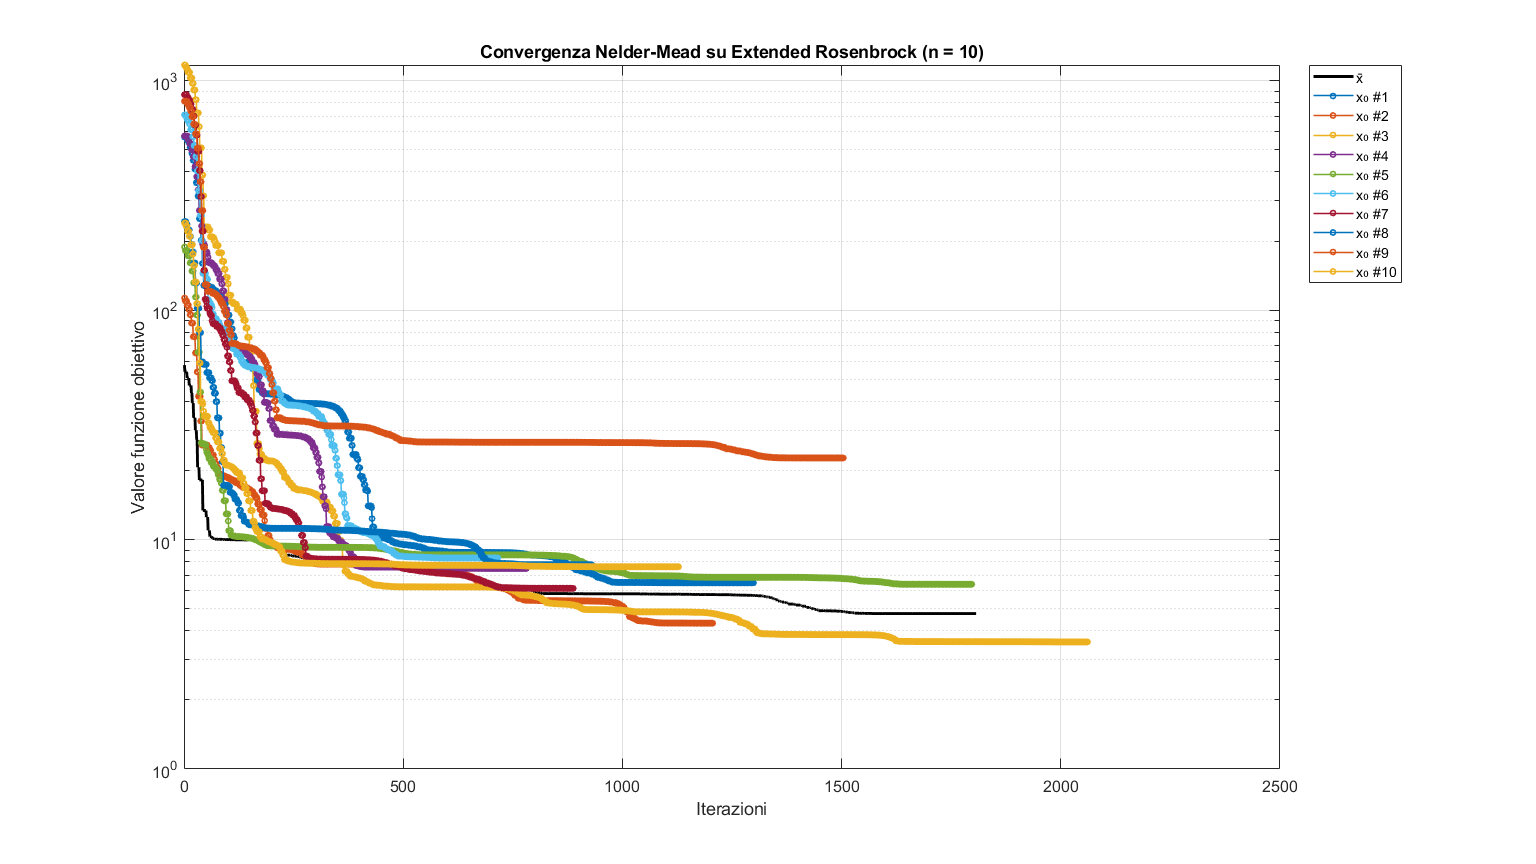
\includegraphics[width=\textwidth]{../immagini/ext_10.png}
		\caption{Convergence of Nelder–Mead on Extended Rosenbrock function ($n=10$) from reference and 10 random initial points. The objective decreases but stagnates above the global minimum.}
		\label{fig:nelder_rosen_10}
	\end{figure}
	
	\begin{figure}[htbp]
		\centering
		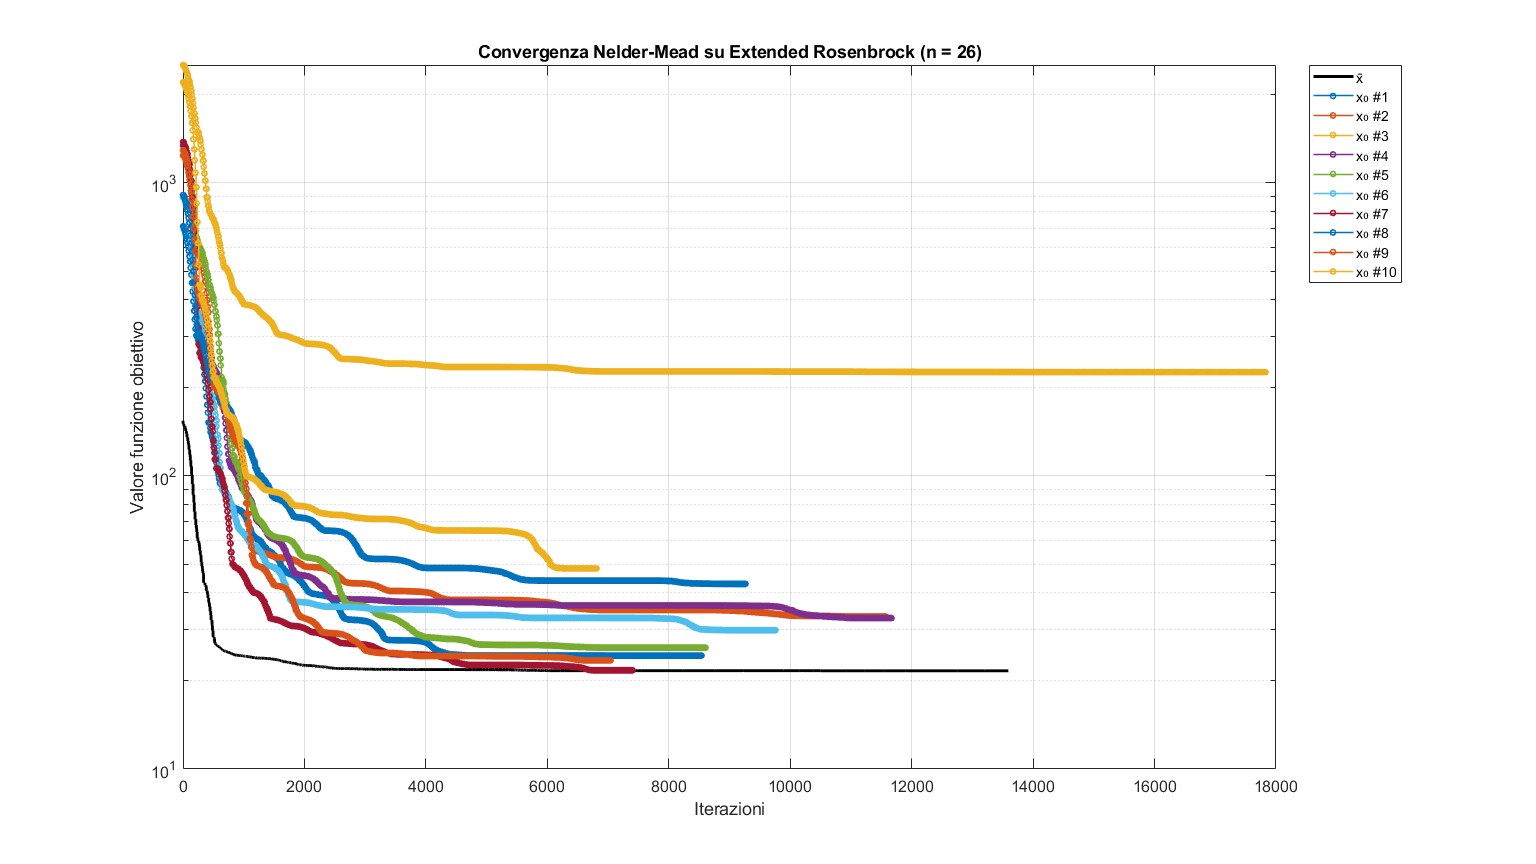
\includegraphics[width=\textwidth]{../immagini/ext_26.png}
		\caption{Convergence of Nelder–Mead on Extended Rosenbrock function ($n=26$). Progress slows down and most trajectories fail to improve after early iterations.}
		\label{fig:nelder_rosen_26}
	\end{figure}
	
	\begin{figure}[htbp]
		\centering
		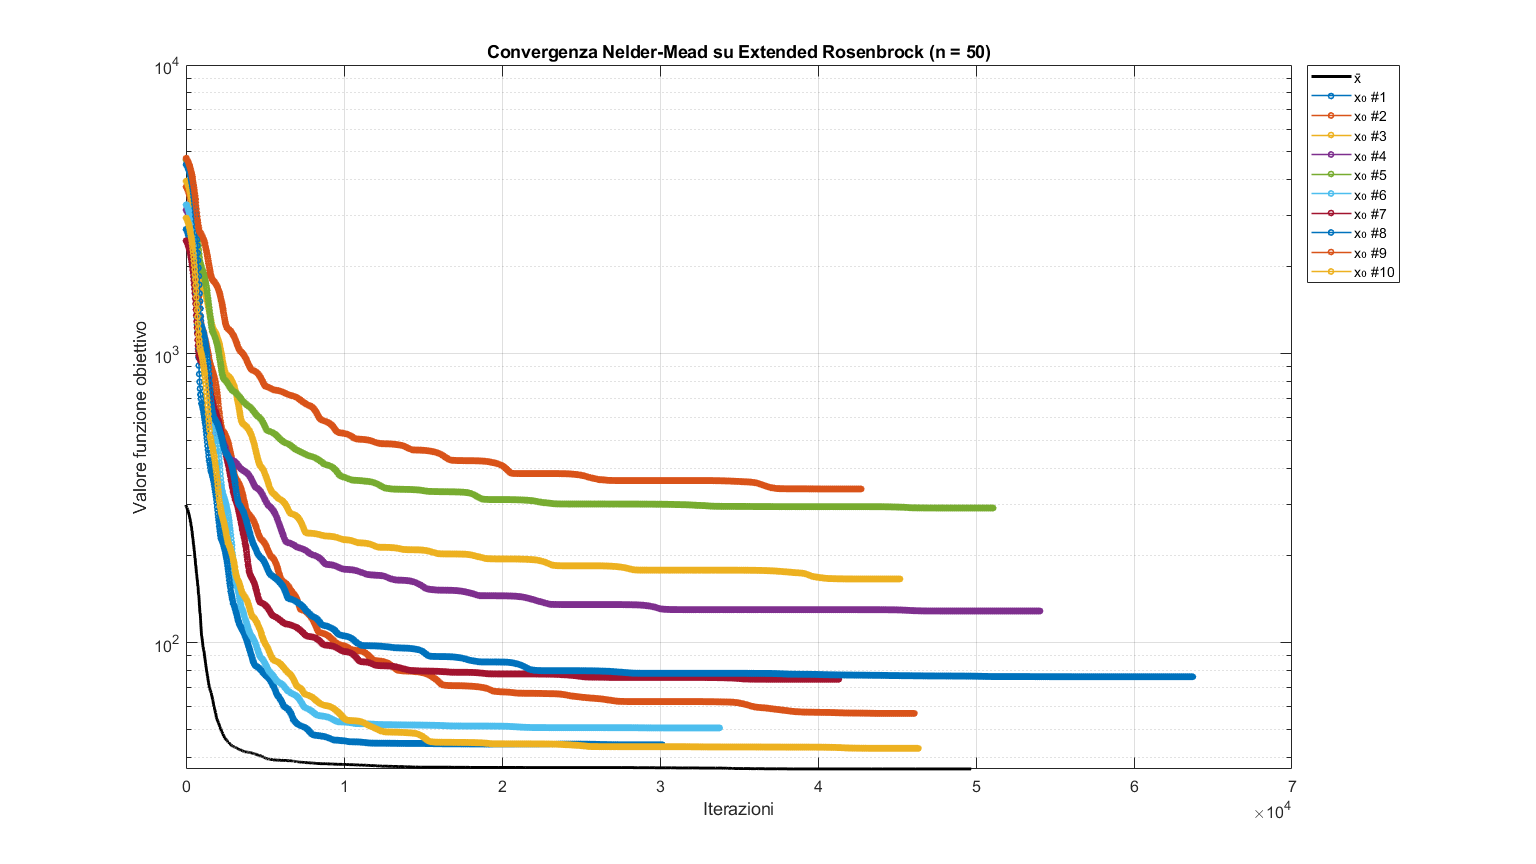
\includegraphics[width=\textwidth]{../immagini/ext_50.png}
		\caption{Convergence of Nelder–Mead on Extended Rosenbrock function ($n=50$). None of the trials reach satisfactory objective values, confirming the method’s limits in high dimensions.}
		\label{fig:nelder_rosen_50}
	\end{figure}
	
	\begin{figure}[H]
		\centering
		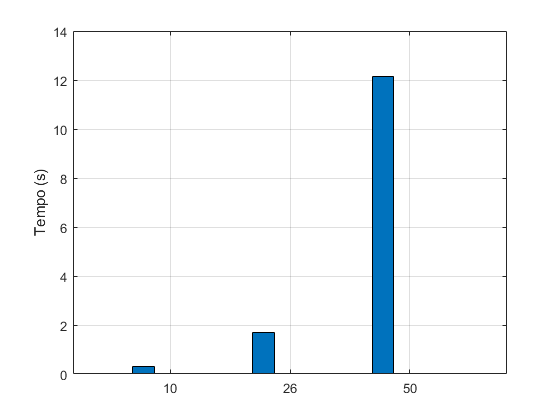
\includegraphics[width=0.6\textwidth]{../immagini/ext_time_nelder.png}
		\caption{Execution time of Nelder–Mead on Extended Rosenbrock for increasing dimensions $n=10$, $26$, and $50$. The cost grows sharply due to the increased simplex size.}
		\label{fig:nelder_rosen_times}
	\end{figure}
	\newpage
	\section{Generalized Broyden Tridiagonal Function}
	\subsection{Problem introduction}
	The Generalized Broyden Tridiagonal function is a classical benchmark used in unconstrained optimization, known for its nonlinear and tridiagonal structure. Let \( x \in \mathbb{R}^{n} \),
	\begin{equation}
		F(x) = \frac{1}{2} \sum_{k=1}^{n} f_k^2(x)
		\qquad\qquad
		f_k(x) = (3 - 2x_k)x_k + 1 - x_{k-1} - x_{k+1},
	\end{equation}
	with boundary conditions \( x_0 = x_{n+1} = 0 \). 
	$F(x)$ combines a quadratic component in \( x_i \), two linear coupling terms with the neighbors \( x_{i-1} \) and \( x_{i+1} \), and adds a constant shift. The global minimum of the function is \( F(x^\star) = 0 \) is achieved when all terms inside the squared expression are zero. Thus, the global minimizer $x^{*} \in$ $\mathbb{R}^{n}$ is such that
	\[
	x_i^{*} = 1, \quad \forall i  = 1,\dots,n.
	\]
	
	\noindent In this chapter we are going to analyze the behaviour of both the Modified Newton and the Nelder–Mead methods, when they are applied to minimize the Generalized Broyden Tridigonal function. 
	The initial points suggested in the benchmark library  are $\bar{x} \in \mathbb{R}^{n}$ such that
	\[
	\bar{x}_{k} = -1.0 \quad \text{for} \quad k = 1,2,\dots n, 		
	\]
	together with another 10 random initial points sampled uniformly in the hypercube $[\bar{x}_{1}-1,\bar{x}_{1}+1]\times\dots\times[\bar{x}_{n}-1,\bar{x}_{n}+1] \subset \mathbb{R}^{n}$, starting from $\bar{x}$.
	
	\begin{figure}[H]
		\centering
		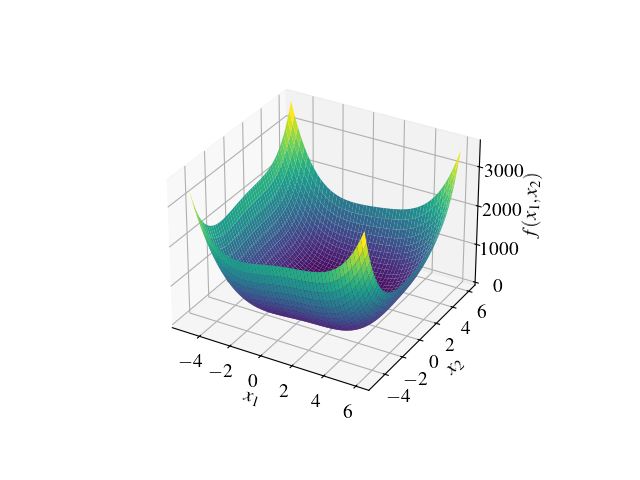
\includegraphics[width=0.65\textwidth]{../immagini/broyden.png}
		\caption{3D visualization of the Generalized Broyden Tridiagonal function for $n=2$.}
		\label{fig:broyden3D}
	\end{figure}
	
	
	\subsection{Modified Newton method}
	In this subsection are shown the results obtained from the minimization of the Generalized Broyden Tridiagonal function using the Modified Newton method; the study includes both exact derivatives and derivatives computed by finite--differences approximations. Due to its pentadiagonal structure, the hessian is stored and manipulated in sparse format; this choice drastically reduces memory requirements and computational cost (in both matrix factorization and Newton direction computation), allowing efficiently handle large--scale problems. Before presenting detailed outcomes, a general experimental setup is given:
	\begin{itemize}
		\item \texttt{n} $= 10^{3},10^{4},10^{5}$;
		\item \texttt{max\_iter} $= 5000$;
		\item \texttt{tol} $= 10^{-6}$.
	\end{itemize}
	
	For each run, the following were tracked:
	\begin{itemize}
		\item number of iterations to convergence;
		\item CPU time;
		\item number of successful runs;
		\item experimental rate of convergence \(\rho\):
		\[
		\rho \approx \frac{\log\left(\|x^{(k+1)} - x^{(k)}\|\big/\|x^{(k)} - x^{(k-1)}\|\right)}{\log\left(\|x^{(k)} - x^{(k-1)}\|\big/\|x^{(k-1)} - x^{(k-2)}\|\right)}.
		\]
		\end{itemize}
	In correspondence with the randomly generated points, an average behavior of each of the previous catogories is reported. Furthermore, the code is designed to work also with finite--differences case,  and this variant is implemented thanks to the extra parameters 
	\begin{itemize}
		\item \texttt{h}: a parameter equal to \(10^{-k} \), for \( k = 2, 4, 6, 8, 10, 12 \);
		\item \texttt{type}: a parameter which indicates if the increment is scaled componentwise as \( h_i = 10^{-k} \cdot |x_i| \) or if it is a default increment such that \( h_i = 10^{-k}\). 
	\end{itemize}
	
	\noindent For this part, the several features were computed for each stepsize h.
	
	\subsubsection{Modified Newton method with exact derivatives}
	
	In this section we test the Modified Newton method on the Generalized Broyden Tridiagonal function using exact gradient and hessian. Both were derived analytically and implemented exploiting the banded pattern of the function. Specifically:
	
	\begin{itemize}
		\item each gradient's component is computed as:
		\[
		\frac{\partial F}{\partial x_k}(x) =
		\begin{cases}
			(3 - 4x_1)f_1(x) - f_2(x), & k = 1 \\
			(3 - 4x_k)f_k(x) - f_{k+1}(x) - f_{k-1}(x), & 1 < k < n \\
			(3 - 4x_n)f_n(x) - f_{n-1}(x), & k = n
		\end{cases};
		\]	
		\item each entry of the hessian is given by:
		\[
		\frac{\partial^2 F}{\partial x_k \partial x_j}(x) =
		\begin{cases}
			(3 - 4x_1)^2 - 4f_1(x) + 1, & k = j = 1 \\
			(3 - 4x_k)^2 - 4f_k(x) + 2, & 1 < k < n,\ k = j \\
			(3 - 4x_n)^2 - 4f_n(x) + 1, & k = j = n \\
			4x_k + 4x_{k+1} - 6, & |k - j| = 1 \\
			1, & |k - j| = 2 \\
			0 & \text{otherwise}
		\end{cases}.
		\]
	\end{itemize}	
		
	%with boundary padding for \( x_0 = x_{n+1} = 0 \). 	
	%It is composed of:
	%\begin{itemize}
	%	\item the main diagonal: second derivatives of each component,
	%	\item the first codiagonals: cross terms with neighboring variables,
	%	\item the second codiagonals: constant contributions from interactions two positions apart.
	%\end{itemize}
	
	
	
	\begin{table}[H]%[htbp]
		\centering
		\renewcommand{\arraystretch}{1.2}
		\begin{tabular}{|c|c|c|c|c|c|}
			\hline
			\textbf{Dim} & \textbf{Init.} & \textbf{$f_{\min}$} & \textbf{Iter} & \textbf{Time (s)} & \textbf{$\rho$} \\
			\hline
			$10^3$   & $\bar{x}$       & $0.000000$  & 5   & 0.02 & 1.93 \\
			& Avg (10 pts)    & $<10^{-6}$  & 8.1 & 0.02 & 1.63 \\
			\hline
			$10^4$   & $\bar{x}$       & $0.000000$  & 5   & 0.17 & 1.93 \\
			& Avg (10 pts)    & $<10^{-6}$  & 8.0 & 0.17 & 1.64 \\
			\hline
			$10^5$   & $\bar{x}$       & $0.000000$  & 5   & 2.01 & 1.93 \\
			& Avg (10 pts)    & $<10^{-6}$  & 8.0 & 2.08 & 1.62 \\
			\hline
		\end{tabular}
		\label{tab:gb_exact_al}
		\caption{Results of Modified Newton method on Generalized Broyden function using exact derivatives.}
	\end{table}
	
	\paragraph{Experimental results.}
	As shown in table (\ref{tab:gb_exact_al}), the Modified Newton method with exact derivatives proves to be extremely effective on the Generalized Broyden tridiagonal function. In all tested dimensions, convergence is achieved in very few iterations (5 for the reference starting point, around 8 on average from random initializations). Function values reach machine precision accuracy, and the convergence rate \(\rho\) consistently approaches the ideal quadratic rate of 2. Importantly, the computational time remains reasonable even for large dimensions, thanks to the efficient sparse implementation of the hessian matrix. These results confirm that when second-order information is available and well--structured, Newton--type methods offer both precision and speed — outperforming derivative-free approaches by a large margin in terms of both accuracy and reliability.
	
	\begin{figure}[H]
		\centering
		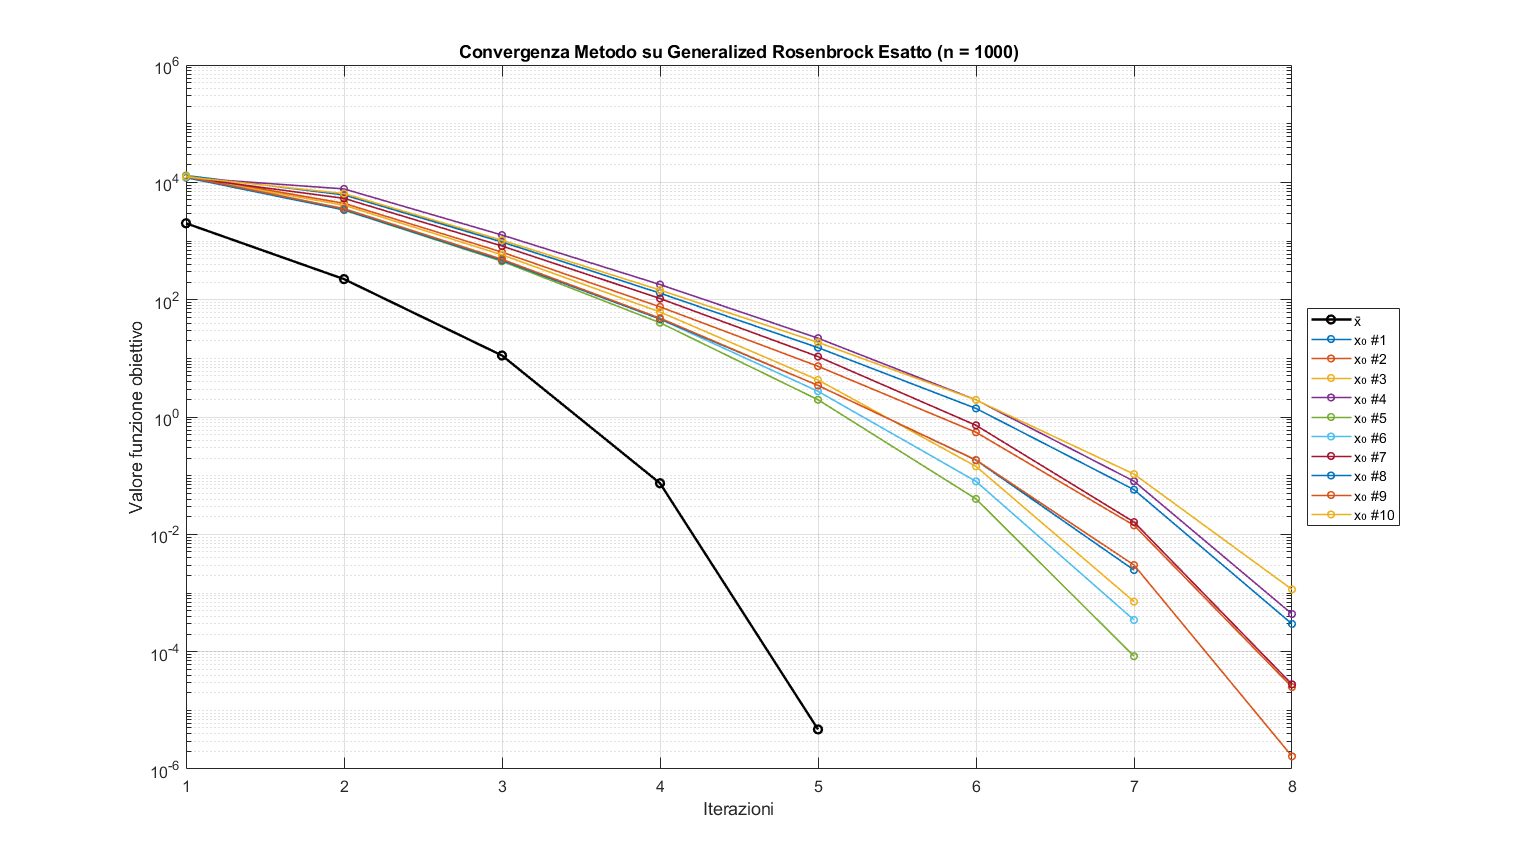
\includegraphics[width=\textwidth]{../immagini/broyden_1k.png}
		\caption{Convergence of the Modified Newton method on Generalized Broyden function with $n=1000$ using exact gradient and Hessian. The method converges in few iterations with a consistent superlinear rate.}
		\label{fig:gb_1k_exact}
	\end{figure}
	
	\begin{figure}[htbp]
		\centering
		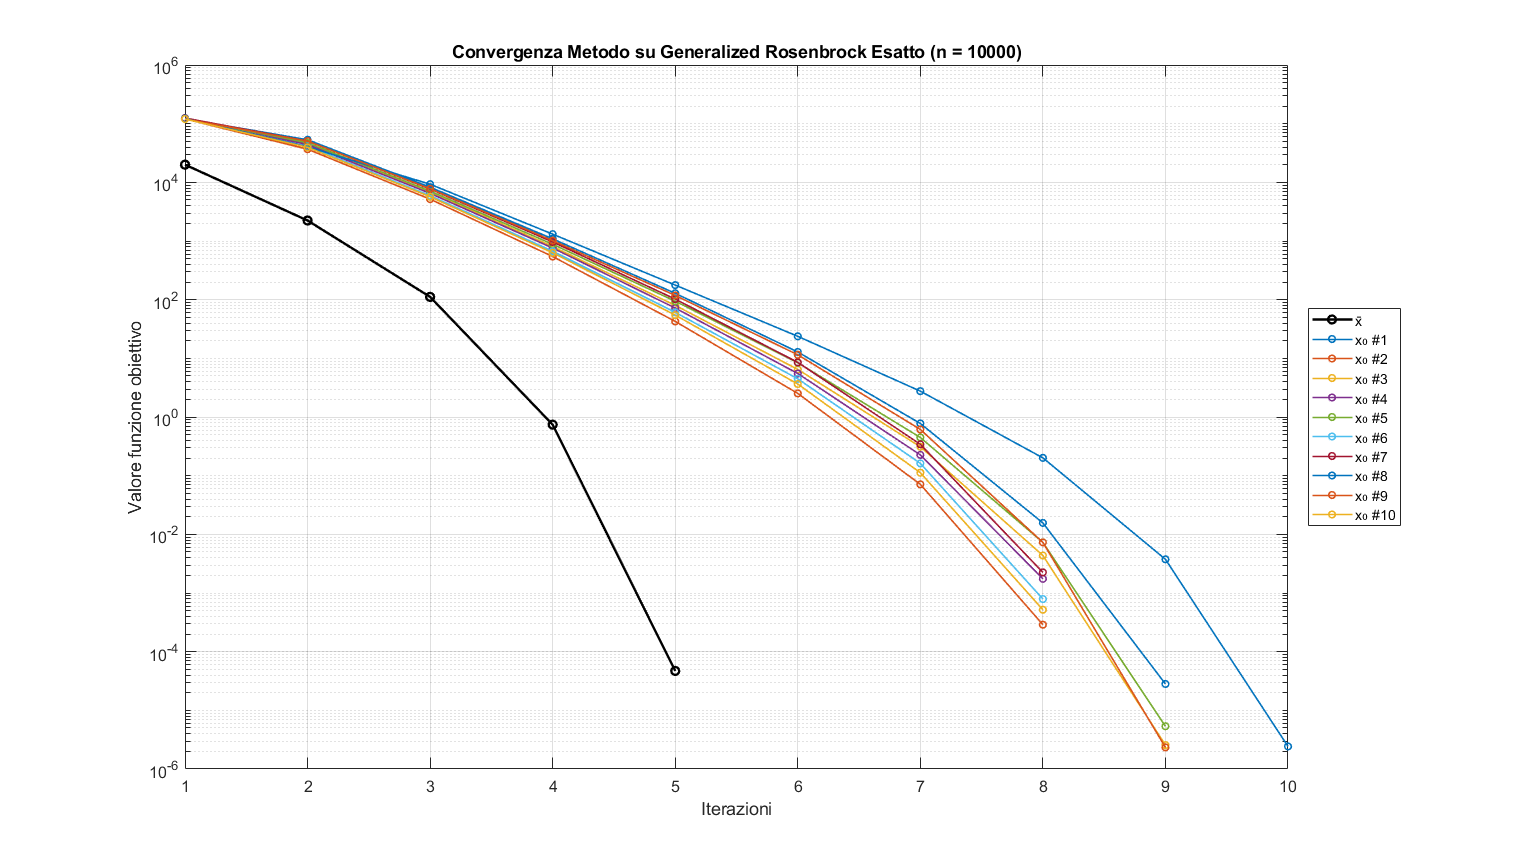
\includegraphics[width=\textwidth]{../immagini/broyden_10k.png}
		\caption{Convergence of the Modified Newton method on Generalized Broyden function with $n=10000$. The convergence behavior remains stable across all random initializations.}
		\label{fig:gb_10k_exact}
	\end{figure}
	
	\begin{figure}[H]
		\centering
		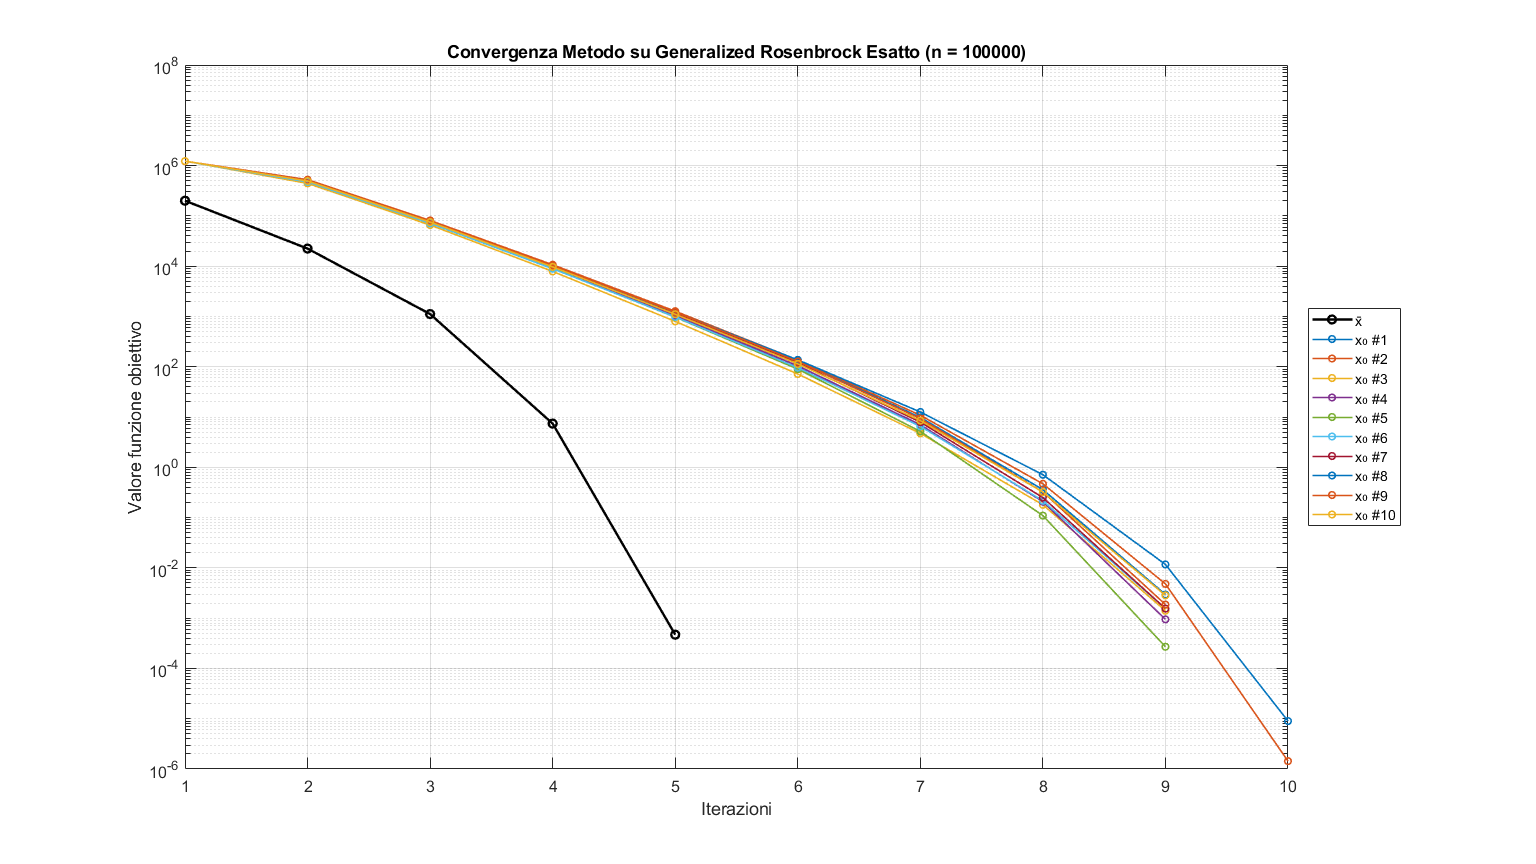
\includegraphics[width=\textwidth]{../immagini/broyden_100k.png}
		\caption{Convergence of the Modified Newton method on Generalized Broyden function with $n=100000$. Even in high dimensions, the algorithm remains robust and fast.}
		\label{fig:gb_100k_exact}
	\end{figure}
	
	\begin{figure}[htbp]
		\centering
		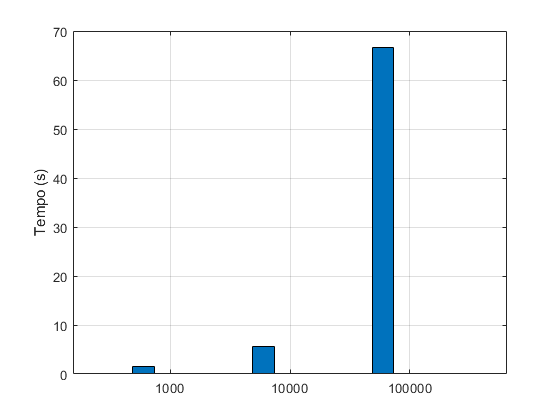
\includegraphics[width=0.6\textwidth]{../immagini/broyden_time_exact.png}
		\caption{Execution time of the Modified Newton method with exact derivatives on Generalized Broyden function for increasing dimensions. The computation scales efficiently due to sparse Hessian structure.}
		\label{fig:gb_time_exact}
	\end{figure}
	
	
	\subsubsection{Modified Newton method with approximated derivatives}
	
	In this experiment, we use the Modified Newton method on the Generalized Broyden Tridiagonal function with gradient and hessian computed via finite differences. This approach avoids symbolic derivation, at the cost of numerical approximations and additional function evaluations. The approximated gradient and Hessian components were expanded manually and implemented directly to avoid cancellation and redundancy. The sparsity pattern of the exact hessian was preserved to limit computational cost.
	
	\vspace{1em}
	
		\paragraph{Gradient approximation.}Due to the structure of the function, only a small number of $f_{k}$ survive when computing the numerator in the formula (\ref{eq1}). In particular, fixed $k$ as the component whose derivative is being approximated, and defining:
	
	\[
	g_{k}(x) = \frac{1}{2}[f^{2}_{k}(x) + f^{2}_{k+1}(x) + f^{2}_{k-1}(x)],
	\]
	then
	\begin{equation}
		\frac{\partial F}{\partial x_{k}}(x) \approx	
			 \frac{g_{k}(x+he_{k}) - g_{k}(x-he_{k})}{2h}.
	\end{equation} 
	
	\noindent It is not reported its explicit expression, as it is corpus. 
	%so
	%\[
	%\begin{cases}
	%6x_1 - 6x_2 + x_3 + 4x_1x_2 + 8x_1h_1^2 - 18x_1^2 %+ 8x_1^3 + 2x_2^2 - 6h_1^2 + 2, & k =1\\
	%2x_1^2 + 4x_1x_2 - 6x_1 + 8x_2^3 - 18x_2^2 + 4x_2x_3 + 8x_2h_2^2 + 7x_2 + 2x_3^2 - 6x_3 - 6h_2^2 + x_0 + x_4 + 1, & 1\leq k \le n \\
	%\end{cases}
	%\]
	
	\paragraph{Hessian approximation.}
	Appling the same proceeding as before, we can observe that function evaluations needed to compute diagonal entries of $\nabla^{2}F(x)$, differ only by the terms 
	\[	
		\frac{1}{2}[f^{2}_{k}(x) + f^{2}_{k+1}(x) + f^{2}_{k-1}(x)].
	\]
	
	\noindent Function evaluations needed to compute non-diagonal entries, on the first codiagonal, differ only by the terms 
	\[
		\frac{1}{2}[f^{2}_{k}(x) + f^{2}_{k+1}(x)],
	\]
	
	\noindent while function evaluations needed to compute the ones on the second codiagonal, differ by the terms
	 \[
	\frac{1}{2}f^{2}_{k-1}(x).
	\]
	 
	\noindent Specifically, the explicit expressions, derived by expanding these differences, are given in the code.
	
	
	\paragraph{Experimental results.}
	In finite differences--case, two figures were generated per dimension: one for fixed and one for scaled increment. As others, each plot contains:
	\begin{itemize}
		\item a black curve for the reference point \( \bar{x} \);
		\item ten colored curves, one for each random starting point;
		\item log--scaled \( f(x_k) \) values against iterations.
	\end{itemize}
	
	\noindent The finite--differences approach is remarkably stable on this problem. All tested step sizes yield convergence in under 30 iterations. Success rates remain at 100\% for all increments, confirming the robustness of the method even in the presence of approximation noise. However, when compared to exact derivatives, the convergence rate \( \rho \) is consistently lower, and runtime increases due to the extra evaluations required. For large--scale problems, this gap grows further due to the cost of computing full gradients and hessians numerically. Overall, this shows that while finite differences can provide reliable optimization results, they are computationally expensive and less efficient than analytical derivatives, when available.
	\noindent Below are the results, divided by problem size.
	\newpage
	\begin{itemize}
	
	\item \boldmath $n = 1\,000$ \unboldmath
	\begin{table}[H]
		\centering
		\renewcommand{\arraystretch}{1.2}
		\resizebox{\textwidth}{!}{%
			\begin{tabular}{|c|c|c|c|c|c|}
				\hline
				\textbf{Increment} & \textbf{Init.} & \textbf{Iter} & \textbf{Time (s)} & \textbf{$\rho$} & \textbf{Successes} \\
				\hline
				$10^{-2}$ & $\bar{x}$ & 11 & 0.04 & 0.0216 & 1/1 \\
				$10^{-2}$ & Avg (10 pts) & 8.6 & 0.01 & 0.1495 & 10/10 \\
				$10^{-2}\cdot|x|$ & $\bar{x}$ & 11 & 0.01 & 1.0263 & 1/1 \\
				$10^{-2}\cdot|x|$ & Avg (10 pts) & 8.2 & 0.00 & 0.9274 & 10/10 \\
				\hline
				$10^{-4}$ & $\bar{x}$ & 10 & 0.00 & 1.6064 & 1/1 \\
				$10^{-4}$ & Avg (10 pts) & 7.7 & 0.00 & 1.6201 & 10/10 \\
				$10^{-4}\cdot|x|$ & $\bar{x}$ & 10 & 0.00 & 1.6122 & 1/1 \\
				$10^{-4}\cdot|x|$ & Avg (10 pts) & 7.7 & 0.00 & 1.6200 & 10/10 \\
				\hline
				$10^{-6}$ & $\bar{x}$ & 10 & 0.00 & 1.6112 & 1/1 \\
				$10^{-6}$ & Avg (10 pts) & 7.7 & 0.00 & 1.6200 & 10/10 \\
				$10^{-6}\cdot|x|$ & $\bar{x}$ & 10 & 0.00 & 1.6113 & 1/1 \\
				$10^{-6}\cdot|x|$ & Avg (10 pts) & 7.7 & 0.00 & 1.6200 & 10/10 \\
				\hline
				$10^{-8}$ & $\bar{x}$ & 10 & 0.00 & 1.6113 & 1/1 \\
				$10^{-8}$ & Avg (10 pts) & 7.7 & 0.00 & 1.6200 & 10/10 \\
				$10^{-8}\cdot|x|$ & $\bar{x}$ & 10 & 0.00 & 1.6113 & 1/1 \\
				$10^{-8}\cdot|x|$ & Avg (10 pts) & 7.7 & 0.00 & 1.6200 & 10/10 \\
				\hline
				$10^{-10}$ & $\bar{x}$ & 10 & 0.00 & 1.6113 & 1/1 \\
				$10^{-10}$ & Avg (10 pts) & 7.7 & 0.00 & 1.6200 & 10/10 \\
				$10^{-10}\cdot|x|$ & $\bar{x}$ & 10 & 0.00 & 1.6113 & 1/1 \\
				$10^{-10}\cdot|x|$ & Avg (10 pts) & 7.7 & 0.00 & 1.6200 & 10/10 \\
				\hline
				$10^{-12}$ & $\bar{x}$ & 10 & 0.00 & 1.6113 & 1/1 \\
				$10^{-12}$ & Avg (10 pts) & 7.7 & 0.00 & 1.6200 & 10/10 \\
				$10^{-12}\cdot|x|$ & $\bar{x}$ & 10 & 0.00 & 1.6113 & 1/1 \\
				$10^{-12}\cdot|x|$ & Avg (10 pts) & 7.7 & 0.00 & 1.6200 & 10/10 \\
				\hline
			\end{tabular}%
		}
		\caption{Finite differences results for $n=1000$ using different increments $h$.}
		\label{tab:gb_fd_1000_all}
	\end{table}
	\newpage
	\begin{figure}[H]
		\centering
		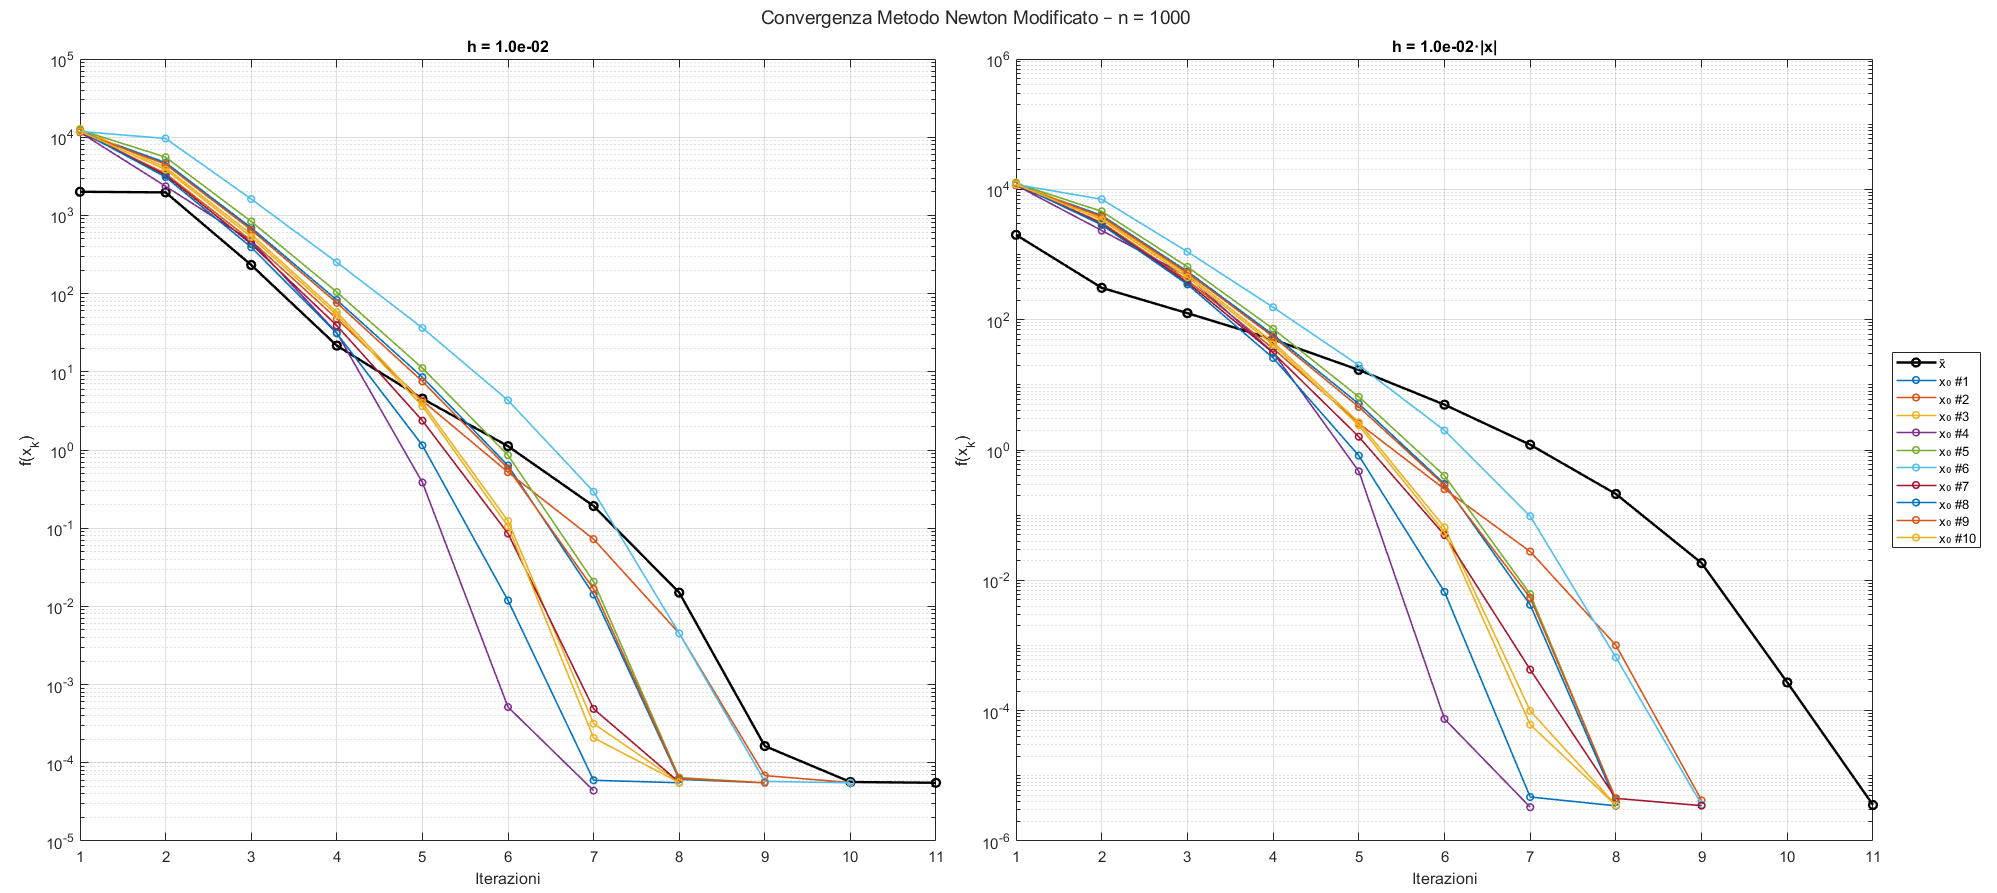
\includegraphics[width=\textwidth]{../immagini/broyden_1k_h2.png}
		\caption{Convergence of Modified Newton method on Generalized Broyden function ($n=1000$) with fixed increment $h = 10^{-2}$ (left) and scaled increment $h = 10^{-2}\cdot|x|$ (right).}
		\label{fig:fd_broyden_1k_h2}
	\end{figure}
	
	\begin{figure}[htbp]
		\centering
		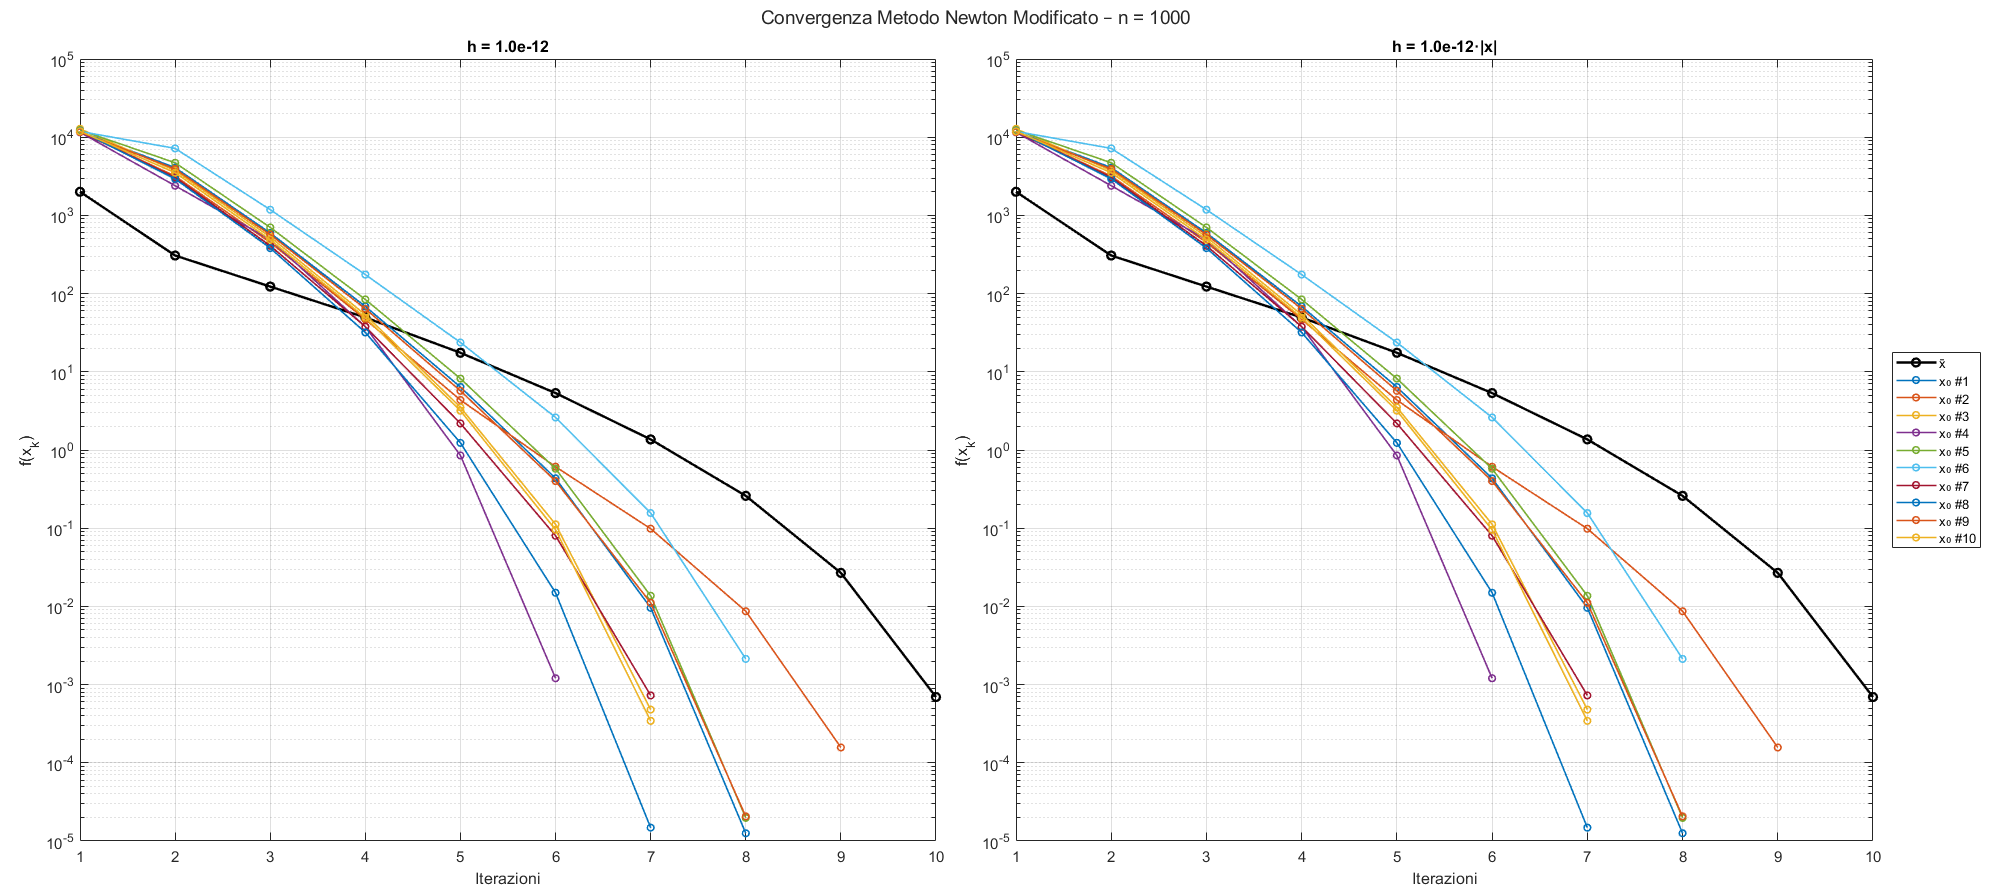
\includegraphics[width=\textwidth]{../immagini/broyden_1k_h12.png}
		\caption{Convergence of Modified Newton method on Generalized Broyden function ($n=1000$) with fixed increment $h = 10^{-12}$ (left) and scaled increment $h = 10^{-12}\cdot|x|$ (right).}
		\label{fig:fd_broyden_1k_h12}
	\end{figure}
	\newpage
	
	\item \boldmath $n = 10\,000$ \unboldmath
	\begin{table}[H]
		\centering
		\renewcommand{\arraystretch}{1.2}
		\resizebox{\textwidth}{!}{%
			\begin{tabular}{|c|c|c|c|c|c|}
				\hline
				\textbf{Increment} & \textbf{Init.} & \textbf{Iter} & \textbf{Time (s)} & \textbf{$\rho$} & \textbf{Successes} \\
				\hline
				$10^{-2}$ & $\bar{x}$ & 12 & 0.04 & 0.0014 & 1/1 \\
				$10^{-2}$ & Avg (10 pts) & 9.4 & 0.04 & 0.0629 & 10/10 \\
				$10^{-2}\cdot|x|$ & $\bar{x}$ & 11 & 0.03 & 0.5256 & 1/1 \\
				$10^{-2}\cdot|x|$ & Avg (10 pts) & 9.4 & 0.04 & 0.4660 & 10/10 \\
				\hline
				$10^{-4}$ & $\bar{x}$ & 10 & 0.03 & 1.6064 & 1/1 \\
				$10^{-4}$ & Avg (10 pts) & 8.5 & 0.03 & 1.5916 & 10/10 \\
				$10^{-4}\cdot|x|$ & $\bar{x}$ & 10 & 0.03 & 1.6122 & 1/1 \\
				$10^{-4}\cdot|x|$ & Avg (10 pts) & 8.5 & 0.03 & 1.5916 & 10/10 \\
				\hline
				$10^{-6}$ & $\bar{x}$ & 10 & 0.03 & 1.6112 & 1/1 \\
				$10^{-6}$ & Avg (10 pts) & 8.5 & 0.03 & 1.5916 & 10/10 \\
				$10^{-6}\cdot|x|$ & $\bar{x}$ & 10 & 0.03 & 1.6113 & 1/1 \\
				$10^{-6}\cdot|x|$ & Avg (10 pts) & 8.5 & 0.03 & 1.5916 & 10/10 \\
				\hline
				$10^{-8}$ & $\bar{x}$ & 10 & 0.03 & 1.6113 & 1/1 \\
				$10^{-8}$ & Avg (10 pts) & 8.5 & 0.03 & 1.5916 & 10/10 \\
				$10^{-8}\cdot|x|$ & $\bar{x}$ & 10 & 0.03 & 1.6113 & 1/1 \\
				$10^{-8}\cdot|x|$ & Avg (10 pts) & 8.5 & 0.03 & 1.5916 & 10/10 \\
				\hline
				$10^{-10}$ & $\bar{x}$ & 10 & 0.03 & 1.6113 & 1/1 \\
				$10^{-10}$ & Avg (10 pts) & 8.5 & 0.03 & 1.5916 & 10/10 \\
				$10^{-10}\cdot|x|$ & $\bar{x}$ & 10 & 0.03 & 1.6113 & 1/1 \\
				$10^{-10}\cdot|x|$ & Avg (10 pts) & 8.5 & 0.03 & 1.5916 & 10/10 \\
				\hline
				$10^{-12}$ & $\bar{x}$ & 10 & 0.03 & 1.6113 & 1/1 \\
				$10^{-12}$ & Avg (10 pts) & 8.5 & 0.03 & 1.5916 & 10/10 \\
				$10^{-12}\cdot|x|$ & $\bar{x}$ & 10 & 0.03 & 1.6113 & 1/1 \\
				$10^{-12}\cdot|x|$ & Avg (10 pts) & 8.5 & 0.03 & 1.5916 & 10/10 \\
				\hline
			\end{tabular}%
		}
		\label{tab:gb_fd_10000}
		\caption{Finite difference results for $n=10\,000$ using different increments $h$.}
	\end{table}
	
	
	\begin{figure}[htbp]
		\centering
		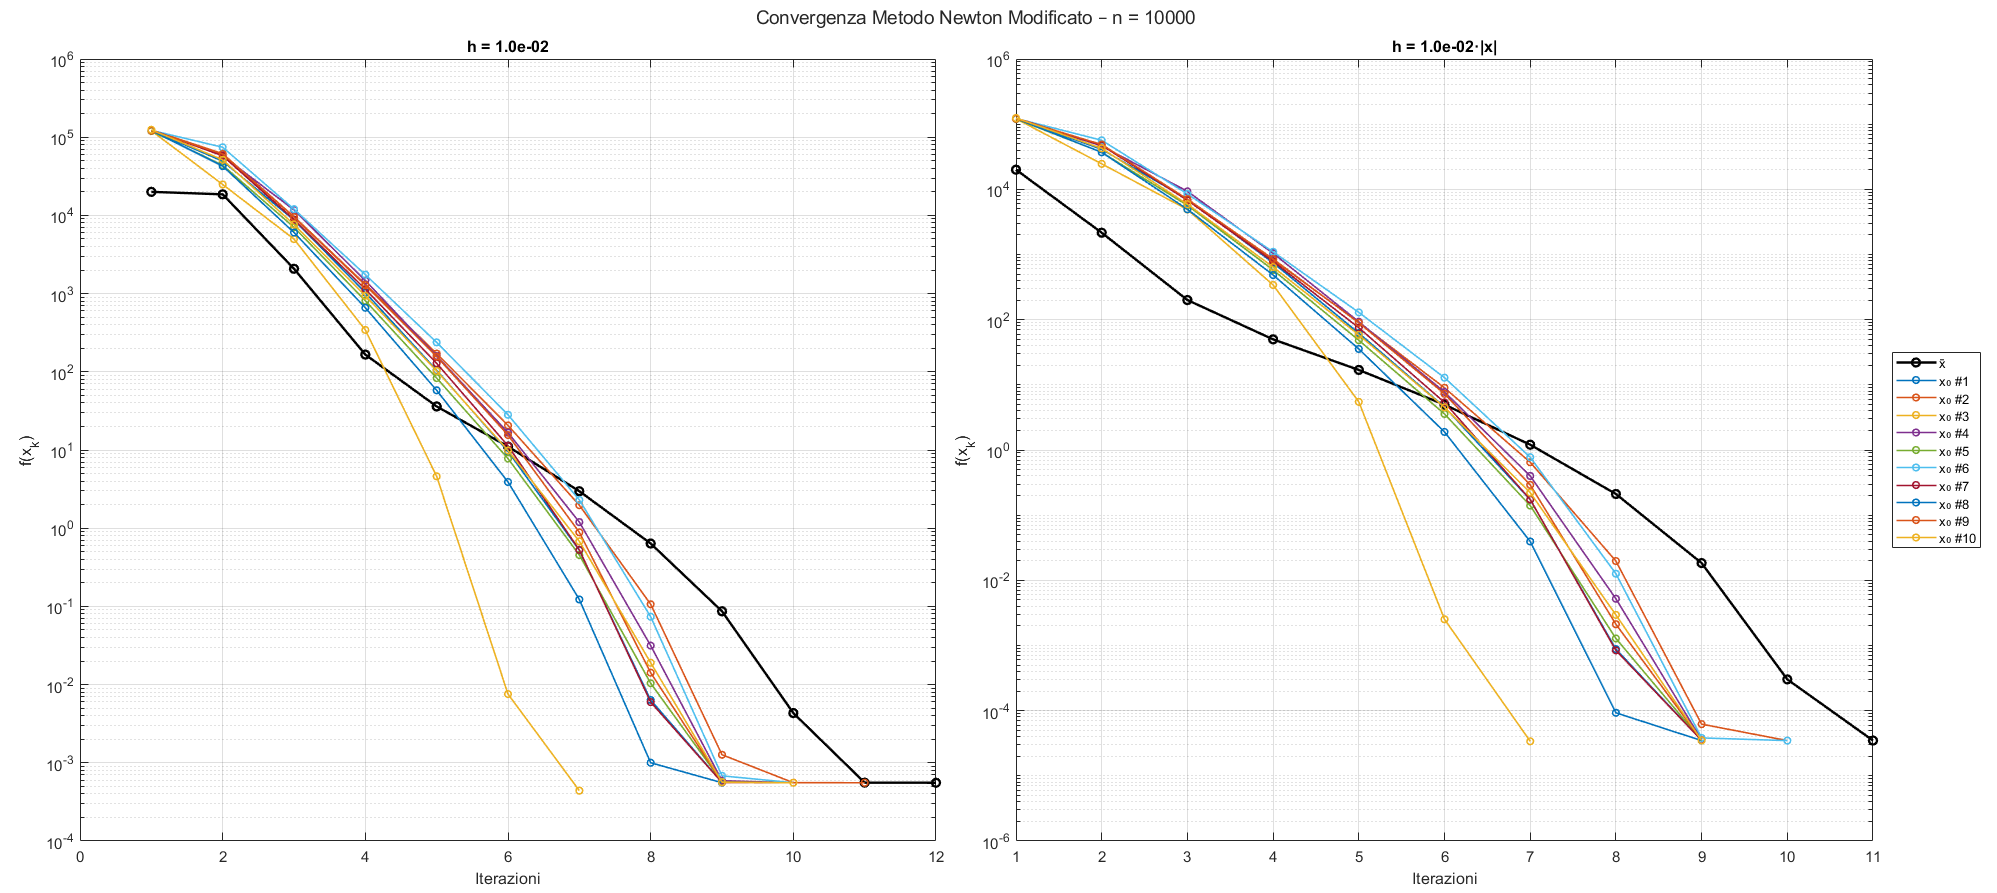
\includegraphics[width=\textwidth]{../immagini/broyden_10k_h2.png}
		\caption{Convergence of Modified Newton method on Generalized Broyden function ($n=10000$) with fixed increment $h = 10^{-2}$ (left) and scaled increment $h = 10^{-2}\cdot|x|$ (right).}
		\label{fig:fd_broyden_10k_h2}
	\end{figure}
	
	\begin{figure}[htbp]
		\centering
		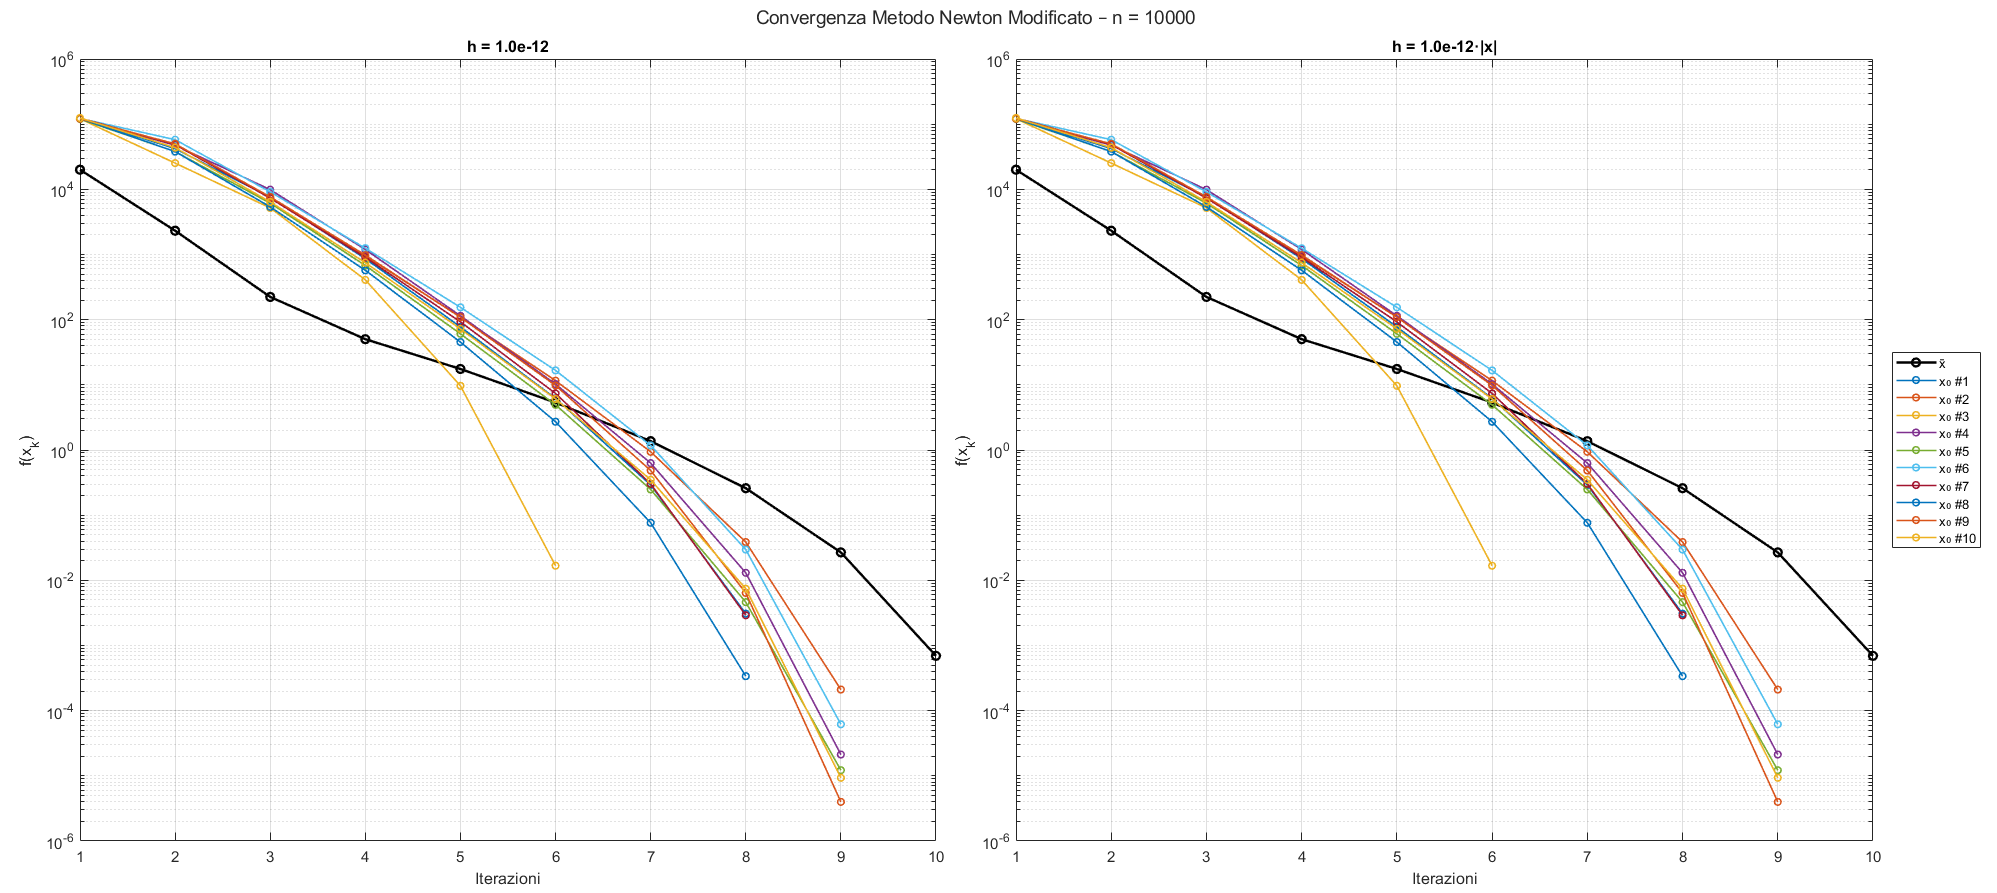
\includegraphics[width=\textwidth]{../immagini/broyden_10k_h12.png}
		\caption{Convergence of Modified Newton method on Generalized Broyden function ($n=10000$) with fixed increment $h = 10^{-12}$ (left) and scaled increment $h = 10^{-12}\cdot|x|$ (right).}
		\label{fig:fd_broyden_10k_h12}
	\end{figure}
	\newpage
	
	\item \boldmath $n = 100\,000$ \unboldmath
	\begin{table}[H]
		\centering
		\renewcommand{\arraystretch}{1.2}
		\resizebox{\textwidth}{!}{%
			\begin{tabular}{|c|c|c|c|c|c|}
				\hline
				\textbf{Increment} & \textbf{Init.} & \textbf{Iter} & \textbf{Time (s)} & \textbf{$\rho$} & \textbf{Successes} \\
				\hline
				$10^{-2}$ & $\bar{x}$ & 14 & 0.51 & 0.0031 & 1/1 \\
				$10^{-2}$ & Avg (10 pts) & 10.9 & 0.56 & 0.0424 & 10/10 \\
				$10^{-2}\cdot|x|$ & $\bar{x}$ & 11 & 0.47 & 0.1670 & 1/1 \\
				$10^{-2}\cdot|x|$ & Avg (10 pts) & 9.6 & 0.49 & 0.1538 & 10/10 \\
				\hline
				$10^{-4}$ & $\bar{x}$ & 10 & 0.36 & 1.6064 & 1/1\\
				$10^{-4}$ & Avg (10 pts) & 8.7 & 0.43 & 1.6182 & 10/10 \\
				$10^{-4}\cdot|x|$ & $\bar{x}$ & 10 & 0.34 & 1.6122 & 1/1 \\
				$10^{-4}\cdot|x|$ & Avg (10 pts) & 8.7 & 0.43 & 1.6173 & 10/10 \\
				\hline
				$10^{-6}$ & $\bar{x}$ & 10 & 0.35 & 1.6112 & 1/1 \\
				$10^{-6}$ & Avg (10 pts) & 8.7 & 0.43 & 1.6171 & 10/10 \\
				$10^{-6}\cdot|x|$ & $\bar{x}$ & 10 & 0.35 & 1.6113 & 1/1 \\
				$10^{-6}\cdot|x|$ & Avg (10 pts) & 8.7 & 0.43 & 1.6170 & 10/10 \\
				\hline
				$10^{-8}$ & $\bar{x}$ & 10 & 0.35 & 1.6113 & 1/1 \\
				$10^{-8}$ & Avg (10 pts) & 8.7 & 0.43 & 1.6170 & 10/10 \\
				$10^{-8}\cdot|x|$ & $\bar{x}$ & 10 & 0.35 & 1.6113 & 1/1 \\
				$10^{-8}\cdot|x|$ & Avg (10 pts) & 8.7 & 0.43 & 1.6170 & 10/10 \\
				\hline
				$10^{-10}$ & $\bar{x}$ & 10 & 0.35 & 1.6113 & 1/1 \\
				$10^{-10}$ & Avg (10 pts) & 8.7 & 0.43 & 1.6170 & 10/10 \\
				$10^{-10}\cdot|x|$ & $\bar{x}$ & 10 & 0.35 & 1.6113 & 1/1 \\
				$10^{-10}\cdot|x|$ & Avg (10 pts) & 8.7 & 0.43 & 1.6170 & 10/10 \\
				\hline
				$10^{-12}$ & $\bar{x}$ & 10 & 0.36 & 1.6113 & 1/1 \\
				$10^{-12}$ & Avg (10 pts) & 8.7 & 0.43 & 1.6170 & 10/10 \\
				$10^{-12}\cdot|x|$ & $\bar{x}$ & 10 & 0.35 & 1.6113 & 1/1 \\
				$10^{-12}\cdot|x|$ & Avg (10 pts) & 8.7 & 0.43 & 1.6170 & 10/10 \\
				\hline
			\end{tabular}%
		}
		\label{tab:gb_fd_100000}
		\caption{Finite difference results for $n=100\,000$ using different increments $h$.}
	\end{table}
	
	\newpage
	\begin{figure}[H]
		\centering
		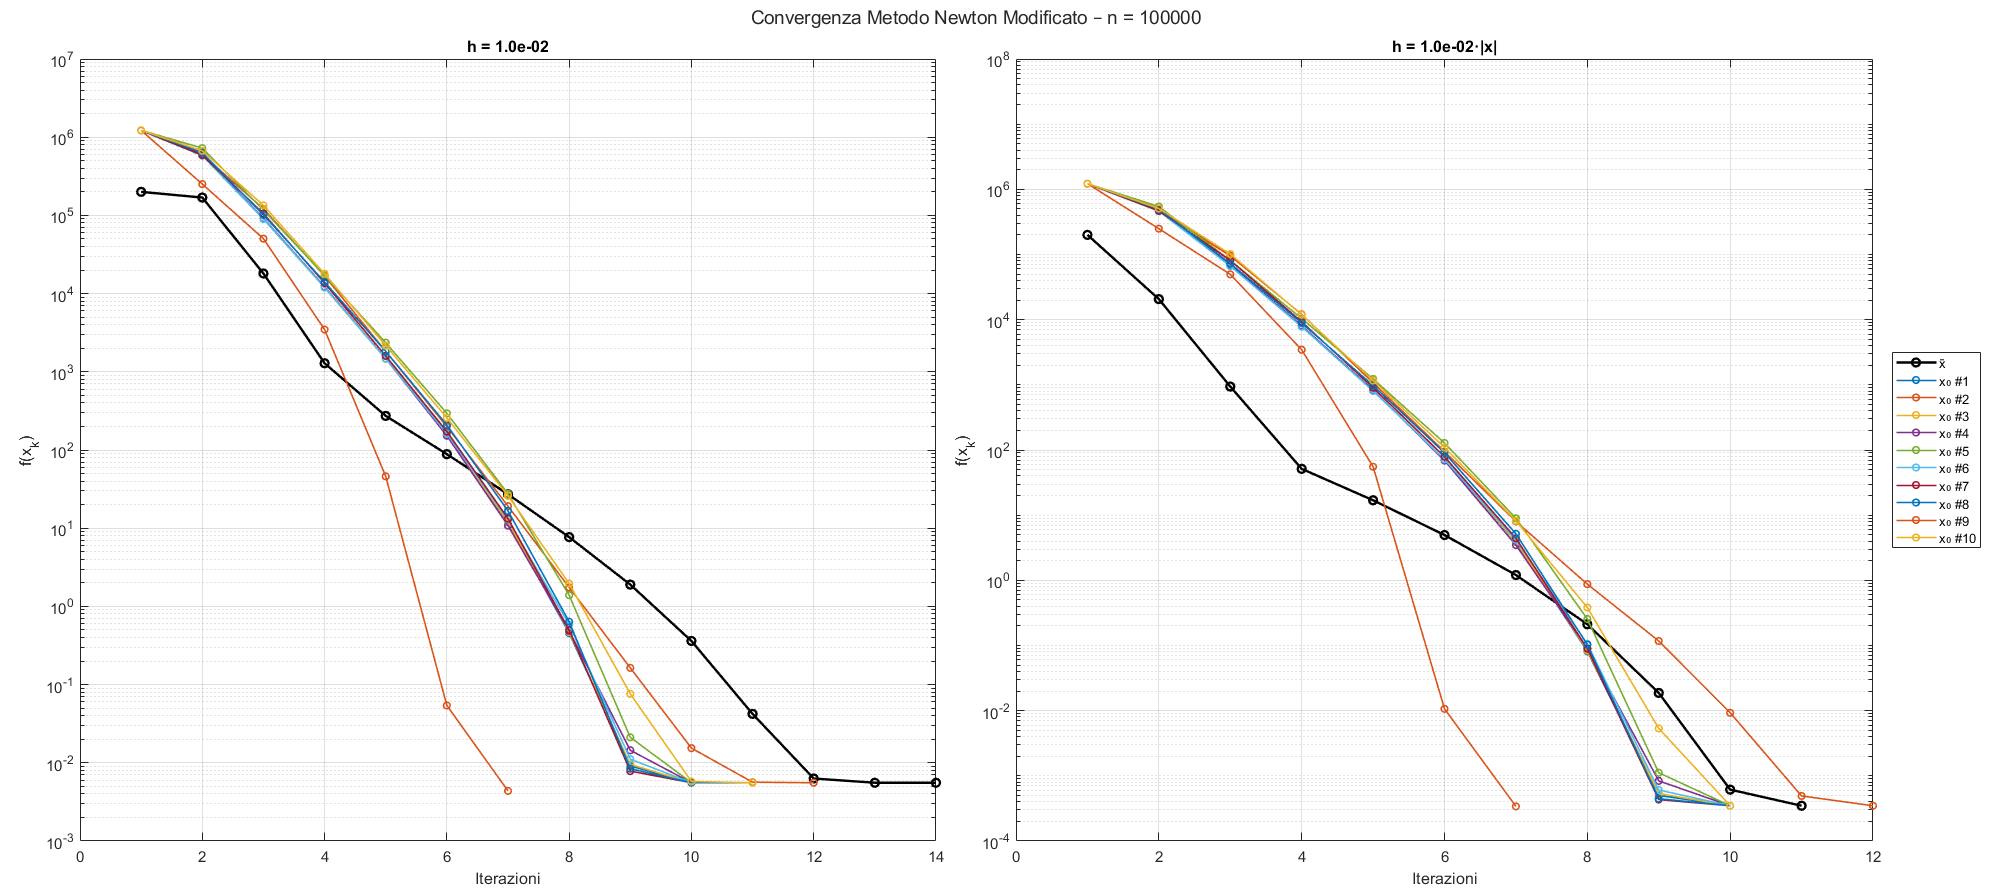
\includegraphics[width=\textwidth]{../immagini/broyden_100k_h2.png}
		\caption{Convergence of Modified Newton method on Generalized Broyden function ($n=100000$) with fixed increment $h = 10^{-2}$ (left) and scaled increment $h = 10^{-2}\cdot|x|$ (right).}
		\label{fig:fd_broyden_100k_h2}
	\end{figure}
	
	\begin{figure}[htbp]
		\centering
		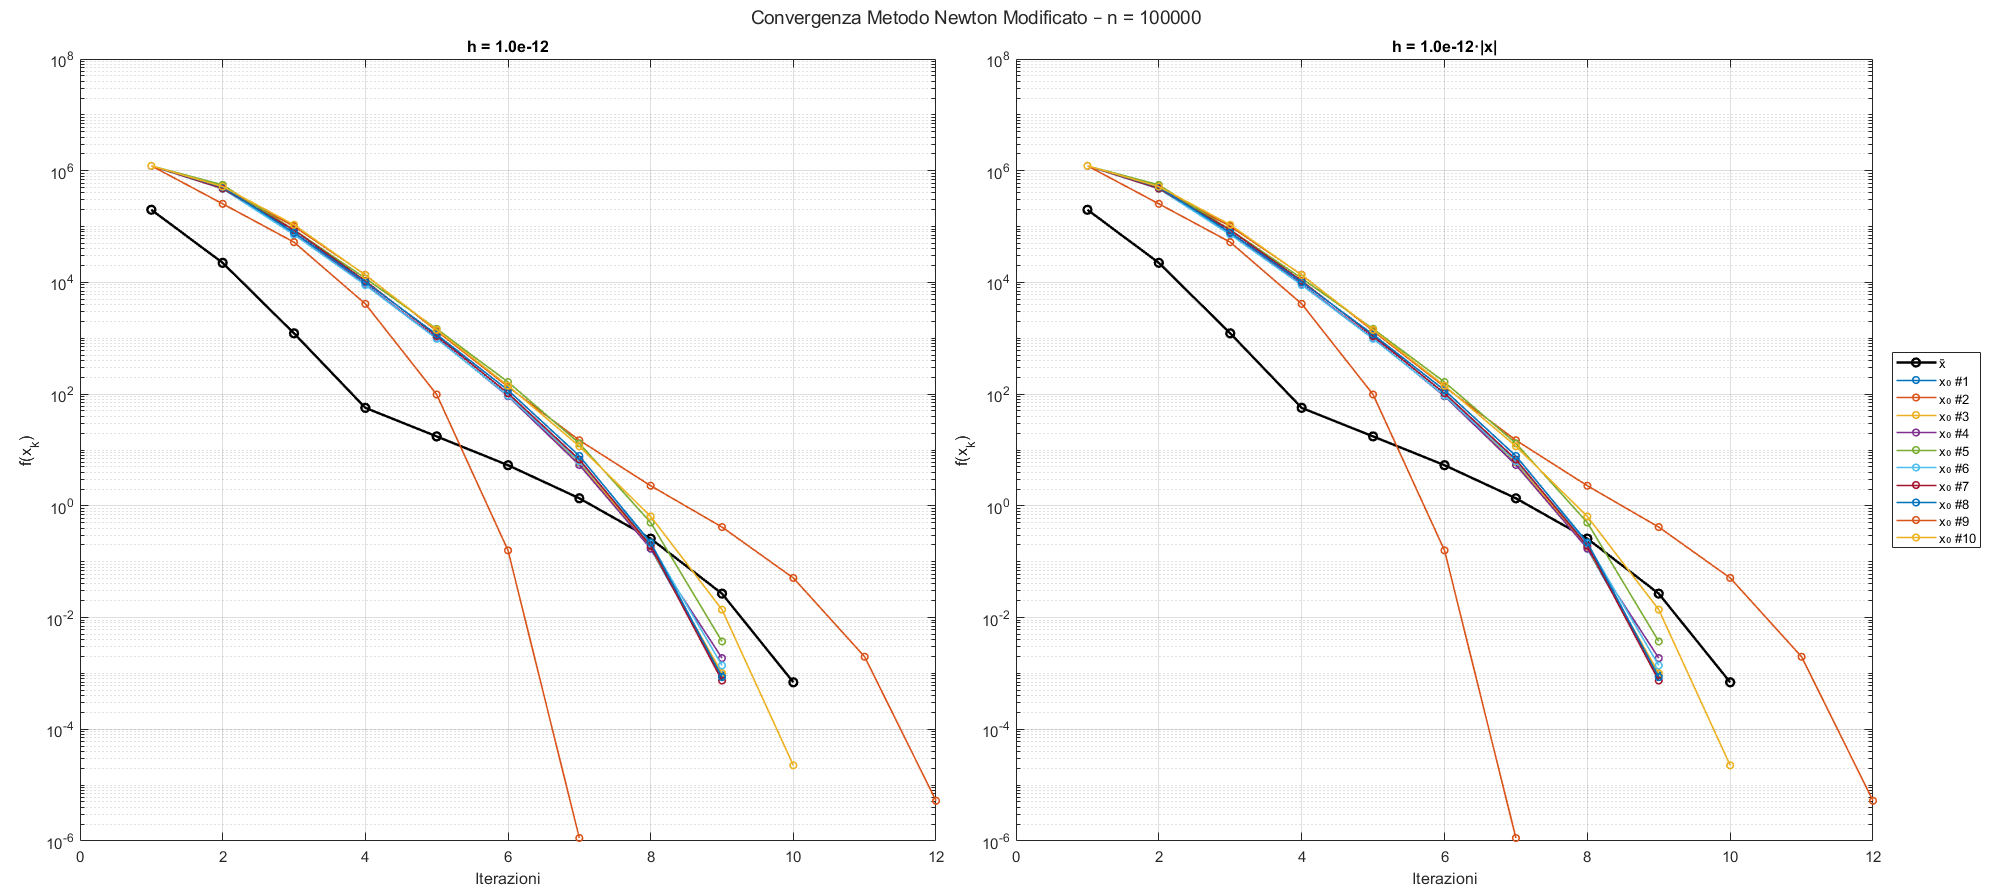
\includegraphics[width=\textwidth]{../immagini/broyden_100k_h12.png}
		\caption{Convergence of Modified Newton method on Generalized Broyden function ($n=100000$) with fixed increment $h = 10^{-12}$ (left) and scaled increment $h = 10^{-12}\cdot|x|$ (right).}
		\label{fig:fd_broyden_100k_h12}
	\end{figure}
	\end{itemize}
	\newpage
		
	\newpage
	
	\subsection{Nelder–Mead method}
	
	In this subsection are shown the results obtained from the minimization of the Generalized Broyden function using the Nelder--Mead method. Before presenting the results, a general experimental setup is given:
	\begin{itemize}
		\item \texttt{n} $= 10, 26, 50$;
		\item \texttt{max\_iter} $= 80.000$;
		\item \texttt{tol} $= 10^{-6}$.
	\end{itemize}
	%	\vspace{0.5cm}
	
	Moreover, for each run have recorded:
	\begin{itemize}
		\item number of iterations to convergence;
		\item CPU time;
		\item final objective value found \(f_{min}\);
		\item experimental rate of convergence \(\rho\):
		\[
		\rho \approx \frac{\log\left(\|x^{(k+1)} - x^{(k)}\|\big/\|x^{(k)} - x^{(k-1)}\|\right)}{\log\left(\|x^{(k)} - x^{(k-1)}\|\big/\|x^{(k-1)} - x^{(k-2)}\|\right)}.
		\]
			\end{itemize}	
	
	In correspondence with the randomly generated points, an average behavior of each of the previous catogories is reported.
	
	\begin{table}[H]
		\renewcommand{\arraystretch}{1.2}
		\resizebox{\textwidth}{!}{%
			\begin{tabular}{|c|c|c|c|c|c|}
				\hline
				\textbf{Dimension} & \textbf{Starting point} & \textbf{$f_{\min}$} & \textbf{Iter} & \textbf{Time (s)} & \textbf{$\rho$} \\
				\hline
				10  & $\bar{x}$         & 0.036184    & 1510   & 0.03 & -1.2743 \\
				& Avg (10 pts)      & 4.974638    & 1467   & 0.018 & 0.3595 \\
				\hline
				26  & $\bar{x}$         & 0.187379    & 7040   & 0.11 & -0.7587 \\
				& Avg (10 pts)      & 45.657701   & 11562  & 0.169 & -3.0863 \\
				\hline
				50  & $\bar{x}$         & 0.206557    & 36027  & 0.83 & -0.6742 \\
				& Avg (10 pts)      & 92.211543   & 52928  & 1.218 & -2.2175 \\
				\hline
			\end{tabular}%
		}
		\caption{Results of Nelder–Mead on Generalized Broyden tridiagonal function.}
		\label{tab:nelder_broyden}
	\end{table}


\paragraph{Experimental results.}

	The Nelder–Mead method performs reasonably well in very low dimensions, such as $n = 10$, where it achieves successful convergence in most runs and a moderate number of iterations. However, as the problem dimension increases, the method becomes significantly less effective. For $n = 25$ and $n = 50$, none of the runs achieved a function value below the target threshold, and both the number of iterations and runtime increase considerably. The convergence rate $\rho$ also becomes unstable, with values indicating erratic or oscillatory behavior. These results highlight the limitations of Nelder–Mead in structured, high-dimensional, non-separable optimization problems, especially when compared to Newton-type methods equipped with derivative information.
	
	\begin{figure}[H]%[htbp]
		\centering
		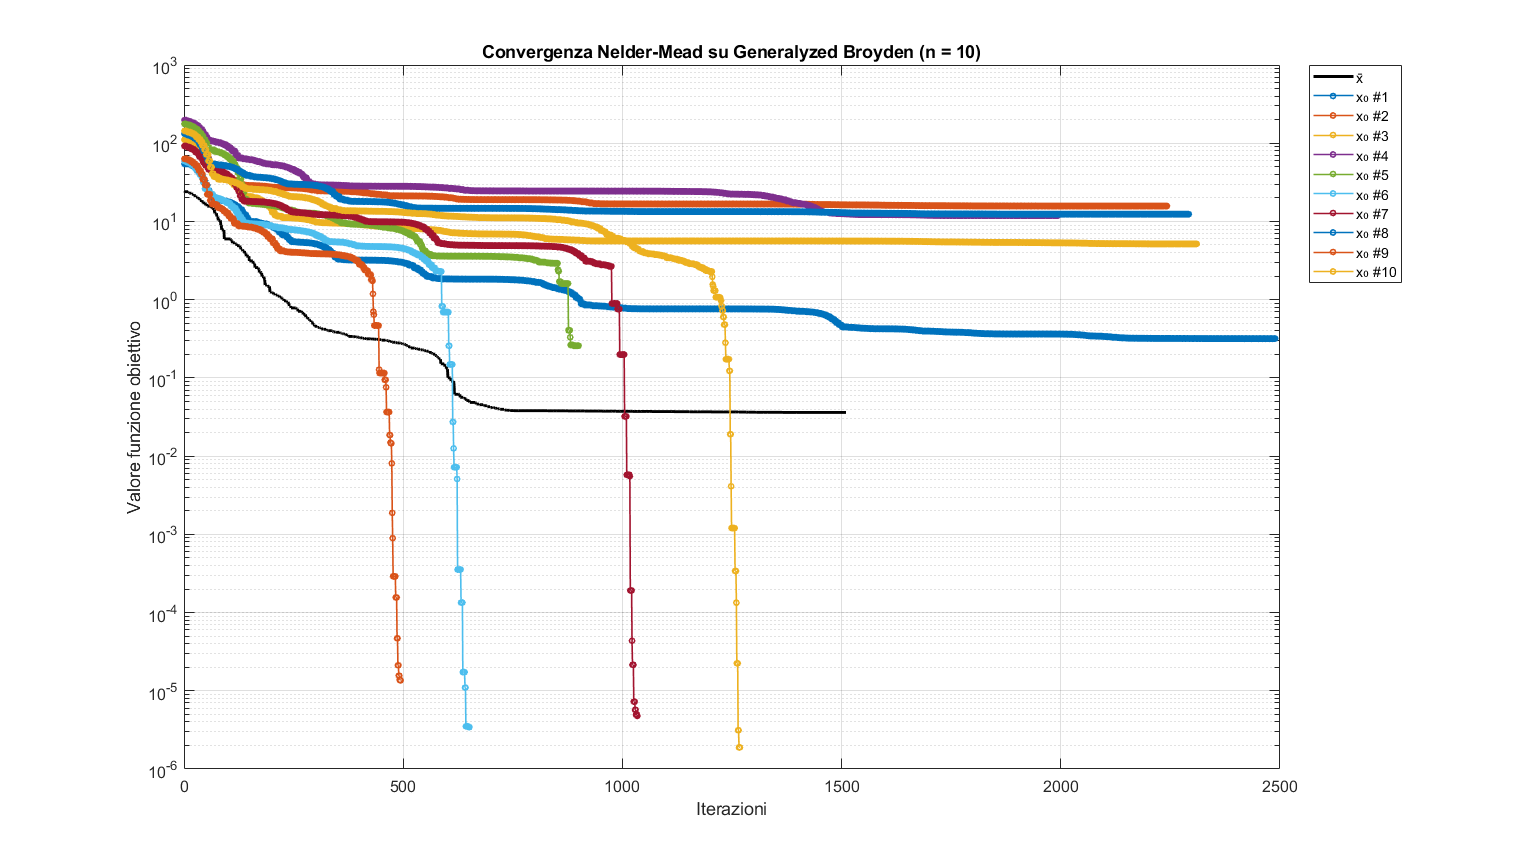
\includegraphics[width=\textwidth]{../immagini/broyden_10.png}
		\caption{Convergence of Nelder-Mead method on Generalized Broyden function ($n=10$) for the reference point $\bar{x}$ (black) and $10$ randomly generated starting points.}
		\label{fig:gb_nelder_10}
	\end{figure}
	\newpage
	\begin{figure}[H]%[htbp]
		\centering
		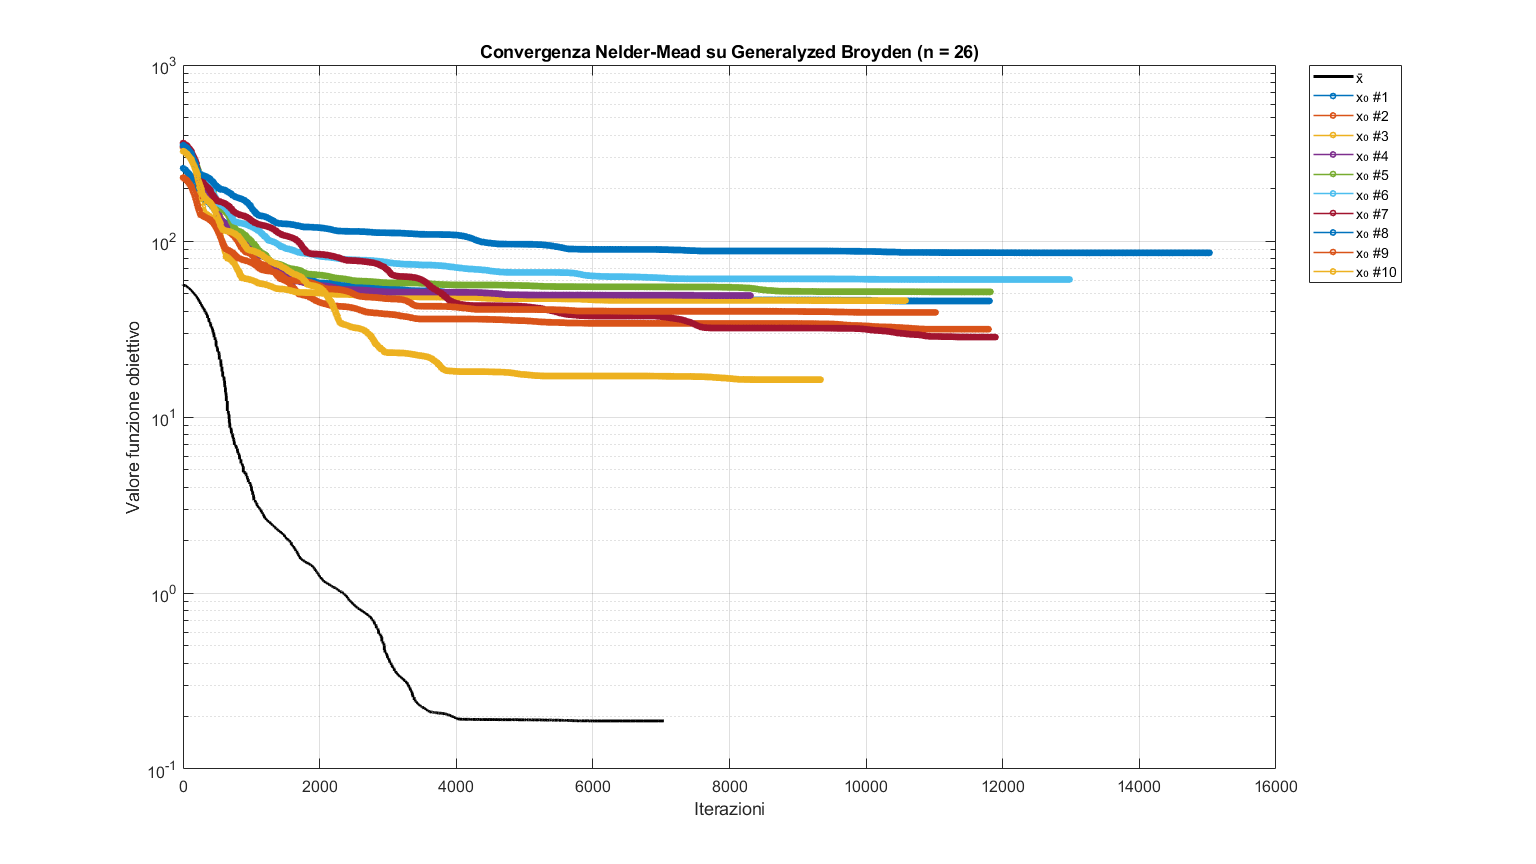
\includegraphics[width=\textwidth]{../immagini/broyden_26.png}
		\caption{Convergence of Nelder-Mead method on Generalized Broyden function ($n=26$) for the reference point $\bar{x}$ (black) and $10$ randomly generated starting points.}
		\label{fig:gb_nelder_26}
	\end{figure}
	
	\begin{figure}[H]%[htbp]
		\centering
		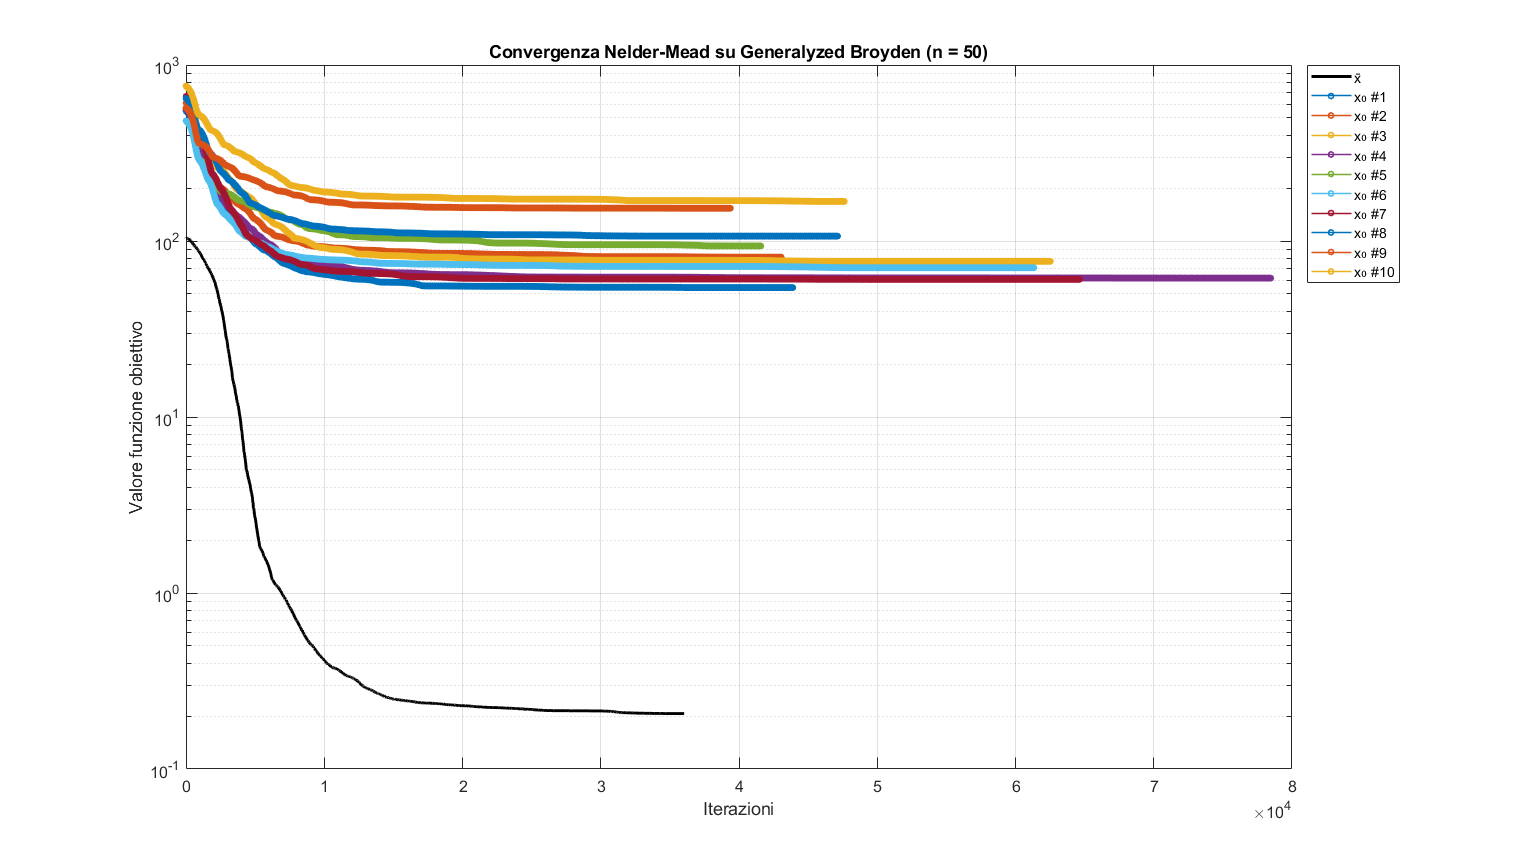
\includegraphics[width=\textwidth]{../immagini/broyden_50.png}
		\caption{Convergence of Nelder-Mead method on Generalized Broyden function ($n=50$) for the reference point $\bar{x}$ (black) and $10$ randomly generated starting points.}
		\label{fig:gb_nelder_50}
	\end{figure}
	
	\begin{figure}[H]%[htbp]
		\centering
		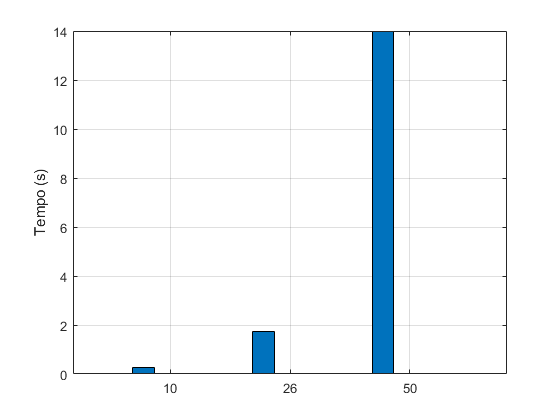
\includegraphics[width=0.6\textwidth]{../immagini/broyden_time_nelder.png}
		\caption{Computational time (in seconds) for Nelder-Mead method applied to the Generalized Broyden function for increasing dimensions.}
		\label{fig:gb_nelder_time}
	\end{figure}
	
	
	\section{Banded Trigonometric Function}
	\subsection{Problem introduction}
	The Banded Trigonometric function is a structured nonlinear objective function characterized by trigonometric dependencies among three consecutive variables. It is defined as:
	
	\[
	f(x) = \sum_{i=1}^{n} i \left[ (1 - \cos(x_i)) + \sin(x_{i-1}) - \sin(x_{i+1}) \right],
	\]
	with boundary conditions \( x_0 = x_{n+1} = 0 \), where \( x \in \mathbb{R}^n \). This objective function arises in problems where local periodic variations influence adjacent terms. Its structure creates a banded dependency pattern, meaning each component interacts only with its two immediate neighbors. Because of the involvement of the sine and cosine trigonometric functions, the Banded Trigonometric function has a single minimum but not a single minimizer, as can be seen in the plot reported in figure (\ref{fig:banded3D}). In this chapter we are going to analyze the behaviour of both the Modified Newton and the Nelder–Mead methods, when they are applied to minimize the Banded Trigonometric function.
	The initial points suggested in the benchmark library  are $\bar{x} \in \mathbb{R}^{n}$ such that
	\[
	\bar{x}_{k} = 1.0 \quad \text{for} \quad k = 1,2,\dots,n,		
	\]
	together with another 10 random initial points sampled uniformly in the hypercube $[\bar{x}_{1}-1,\bar{x}_{1}+1]\times\dots\times[\bar{x}_{n}-1,\bar{x}_{n}+1] \subset \mathbb{R}^{n}$, starting from $\bar{x}$.
	
		\begin{figure}[H]%[htbp]
		\centering
		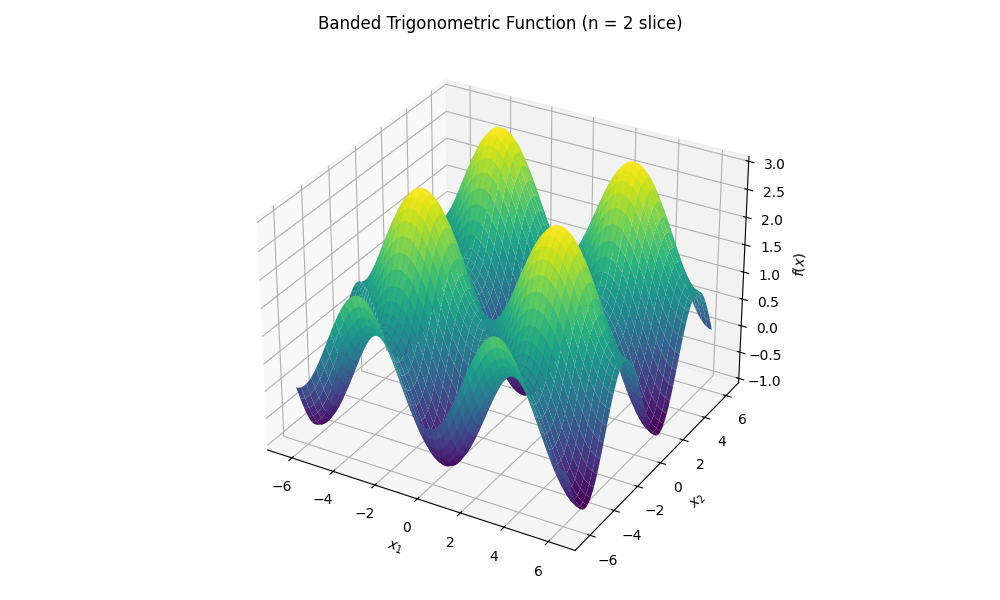
\includegraphics[width=0.65\textwidth]{../immagini/banded_3D.png}
		\caption{3D visualization of the Banded Trigonometric function for $n=2$.}
		\label{fig:banded3D}
	\end{figure}
	
	\newpage
	
	\subsection{Modified Newton method}
	In this subsection are shown the results obtained from the minimization of the Banded Trigonometric function using the Modified Newton method; the study includes both exact derivatives and derivatives computed by finite-differences approximations. Due to its diagonal structure, the hessian is stored and manipulated in sparse format; this choice drastically reduces memory requirements and computational cost (in both matrix factorization and Newton direction computation), allowing efficiently handle large--scale problems.
	
	For this particular function the resulting hessian matrices are often ill-conditioned, especially in higher dimensions. To address this, the Modified Newton method were designed to apply preconditioning through the MATLAB \texttt{pcg} solver (Preconditioned Conjugate Gradient). This choice enables efficient direction computation even when Cholesky factorization becomes unreliable or fails, particularly for large-scale sparse systems.
	The algorithm applies a modified Cholesky approach (Algorithm 6.3 in) to shift the hessian until a positive definite approximation is obtained. Then, an incomplete Cholesky factorization is used to precondition the matrix, ensuring robust convergence even in the presence of large condition numbers.\\
	
	 \noindent Before presenting detailed outcomes, a general experimental setup is given:
	\begin{itemize}
		\item \texttt{n} $= 10^{3},10^{4},10^{5}$;
		\item \texttt{max\_iter} $= 5000$;
		\item \texttt{tol} $= 10^{-6}$;
		\item \texttt{max\_iter\_pcg} $= 50$;
		\item \texttt{tol\_pcg} $= 10^{-6}$;
		\item \texttt{preconditioner\_pcg} $= LL^{T}$, where the factor $L$ is obtained with the incomplete Cholesky factorization of the coefficient matrix.
	\end{itemize}
	\vspace{0.2cm}
	For each run, the following were tracked:
	\begin{itemize}
		\item number of iterations to convergence;
		\item CPU time;
		\item number of successful runs;
		\item experimental rate of convergence \(\rho\):
		\[
		\rho \approx \frac{\log\left(\|x^{(k+1)} - x^{(k)}\|\big/\|x^{(k)} - x^{(k-1)}\|\right)}{\log\left(\|x^{(k)} - x^{(k-1)}\|\big/\|x^{(k-1)} - x^{(k-2)}\|\right)}.
		\]		
	\end{itemize}
	In correspondence with the randomly generated points, an average behavior of each of the previous catogories is reported. It should be emphasized that among the data shown within the tables, rho values approximately equal to or greater than three can be identified. These results are not a correct approximation of the required rate of convergence, as this is at most quadratic in the case of Modified Newton method; These results could be traced to replacing the optimal value of the minimizer with its last available approximation.\\   		
	
	\noindent Furthermore, the code is designed to work also with finite--differences case,  and this variant is implemented thanks to the extra parameters 
	\begin{itemize}
		\item \texttt{h}: a parameter equal to \(10^{-k} \), for \( k = 2, 4, 6, 8, 10, 12 \);
		\item \texttt{type}: a parameter which indicates if the increment is scaled componentwise as \( h_i = 10^{-k} \cdot |x_i| \) or if it is a default increment such that \( h_i = 10^{-k}\). 
	\end{itemize}
	
	\noindent For this part, the several features were computed for each stepsize h.	
	\subsubsection{Modified Newton method with exact derivatives}
		
	In this section the Banded Trigonometric function is minimized using the Modified Newton method with exact gradient and hessian formulas. Both were derived analytically and implemented exploiting the banded pattern of the function. Specifically:

	\begin{itemize}
		\item each gradient's component is constructed as: 
		\[
		\frac{\partial F}{\partial x_k} = 
		\begin{cases}
			\sin(x_{1}) + 2\cos(x_{1}), & i = 1 \\
			k\sin(x_{k}) + 2\cos(x_{k}), & 2 \le k \le n-1 \\
			n\sin(x_n) - (n-1)\cos(x_n), & k = n
		\end{cases};
		\]
		\item each entry of the hessian matrix is computed as:
		\[
		\frac{\partial^2 F}{\partial x_k \partial x_j} = 
		\begin{cases}
			\cos(x_{1}) - 2\sin(x_{1}), & i = 1 \\
			k\cos(x_{k}) - 2\sin(x_{k}), & 2 \le k \le n-1 \\
			n\cos(x_n) + (n-1)\sin(x_n), & i = n\\
			0, &  \text{otherwise}
		\end{cases}.
		\]
		\end{itemize} 
	
	\medskip
	
	\paragraph{Experimental Results.} As shown in table (\ref{tab:banded_exact}), the Modified Newton method with exact derivatives fails in terms of minimizing the Banded Trigonometric function, which turns out to be a particularly challenging function to optimize, if compared to the ones in the other sections. In all dimensions tested and for all initialization points, not only is convergence not satisfied, but the $f_{min}$ values achieved are far from the actual global minimum. Despite preconditioning the hessian matrix during the search for the descent direction, the algorithm fails to reach a value that is reasonably close to the minimum of the function. Below are tables and figures explaining the situation in detail.
	
	\begin{table}[H]%[htbp]
		\centering
		\renewcommand{\arraystretch}{1.2}
		\begin{tabular}{|c|c|c|c|c|c|c|}
			\hline
			\textbf{Dim} & \textbf{Init.} & \textbf{Iter} & \textbf{Time (s)} & \textbf{$f_{\min}$} & \textbf{$\rho$} & \textbf{Successes} \\
			\hline
			$10^3$   & $\bar{x}$        & 6    & 0.04 & $-427.40$     & 2.52 & 1/1 \\
			& Avg (10 pts)     & 16.4 & 0.02 & $-565.12$  & 2.62  & 10/10 \\
			\hline
			$10^4$   & $\bar{x}$        & 7    & 0.04 & $-4159.93$    & 2.22 & 1/1 \\
			& Avg (10 pts)     & 20.4 & 0.22 & $-2835.42$    & 2.25 & 10/10 \\
			\hline
			$10^5$   & $\bar{x}$  & 6    & 0.36 & $-41443.76$   & 4.11 & 1/1 \\
			& Avg (10 pts)     & 29.7 & 4.78 & $-37052.49$   & 1.78 & 10/10 \\
			\hline
		\end{tabular}
		\label{tab:banded_exact}
		\caption{Results of Modified Newton method on Banded Trigonometric function using exact derivatives.}
	\end{table}
	
	\begin{figure}[H]%[htbp]
		\centering
		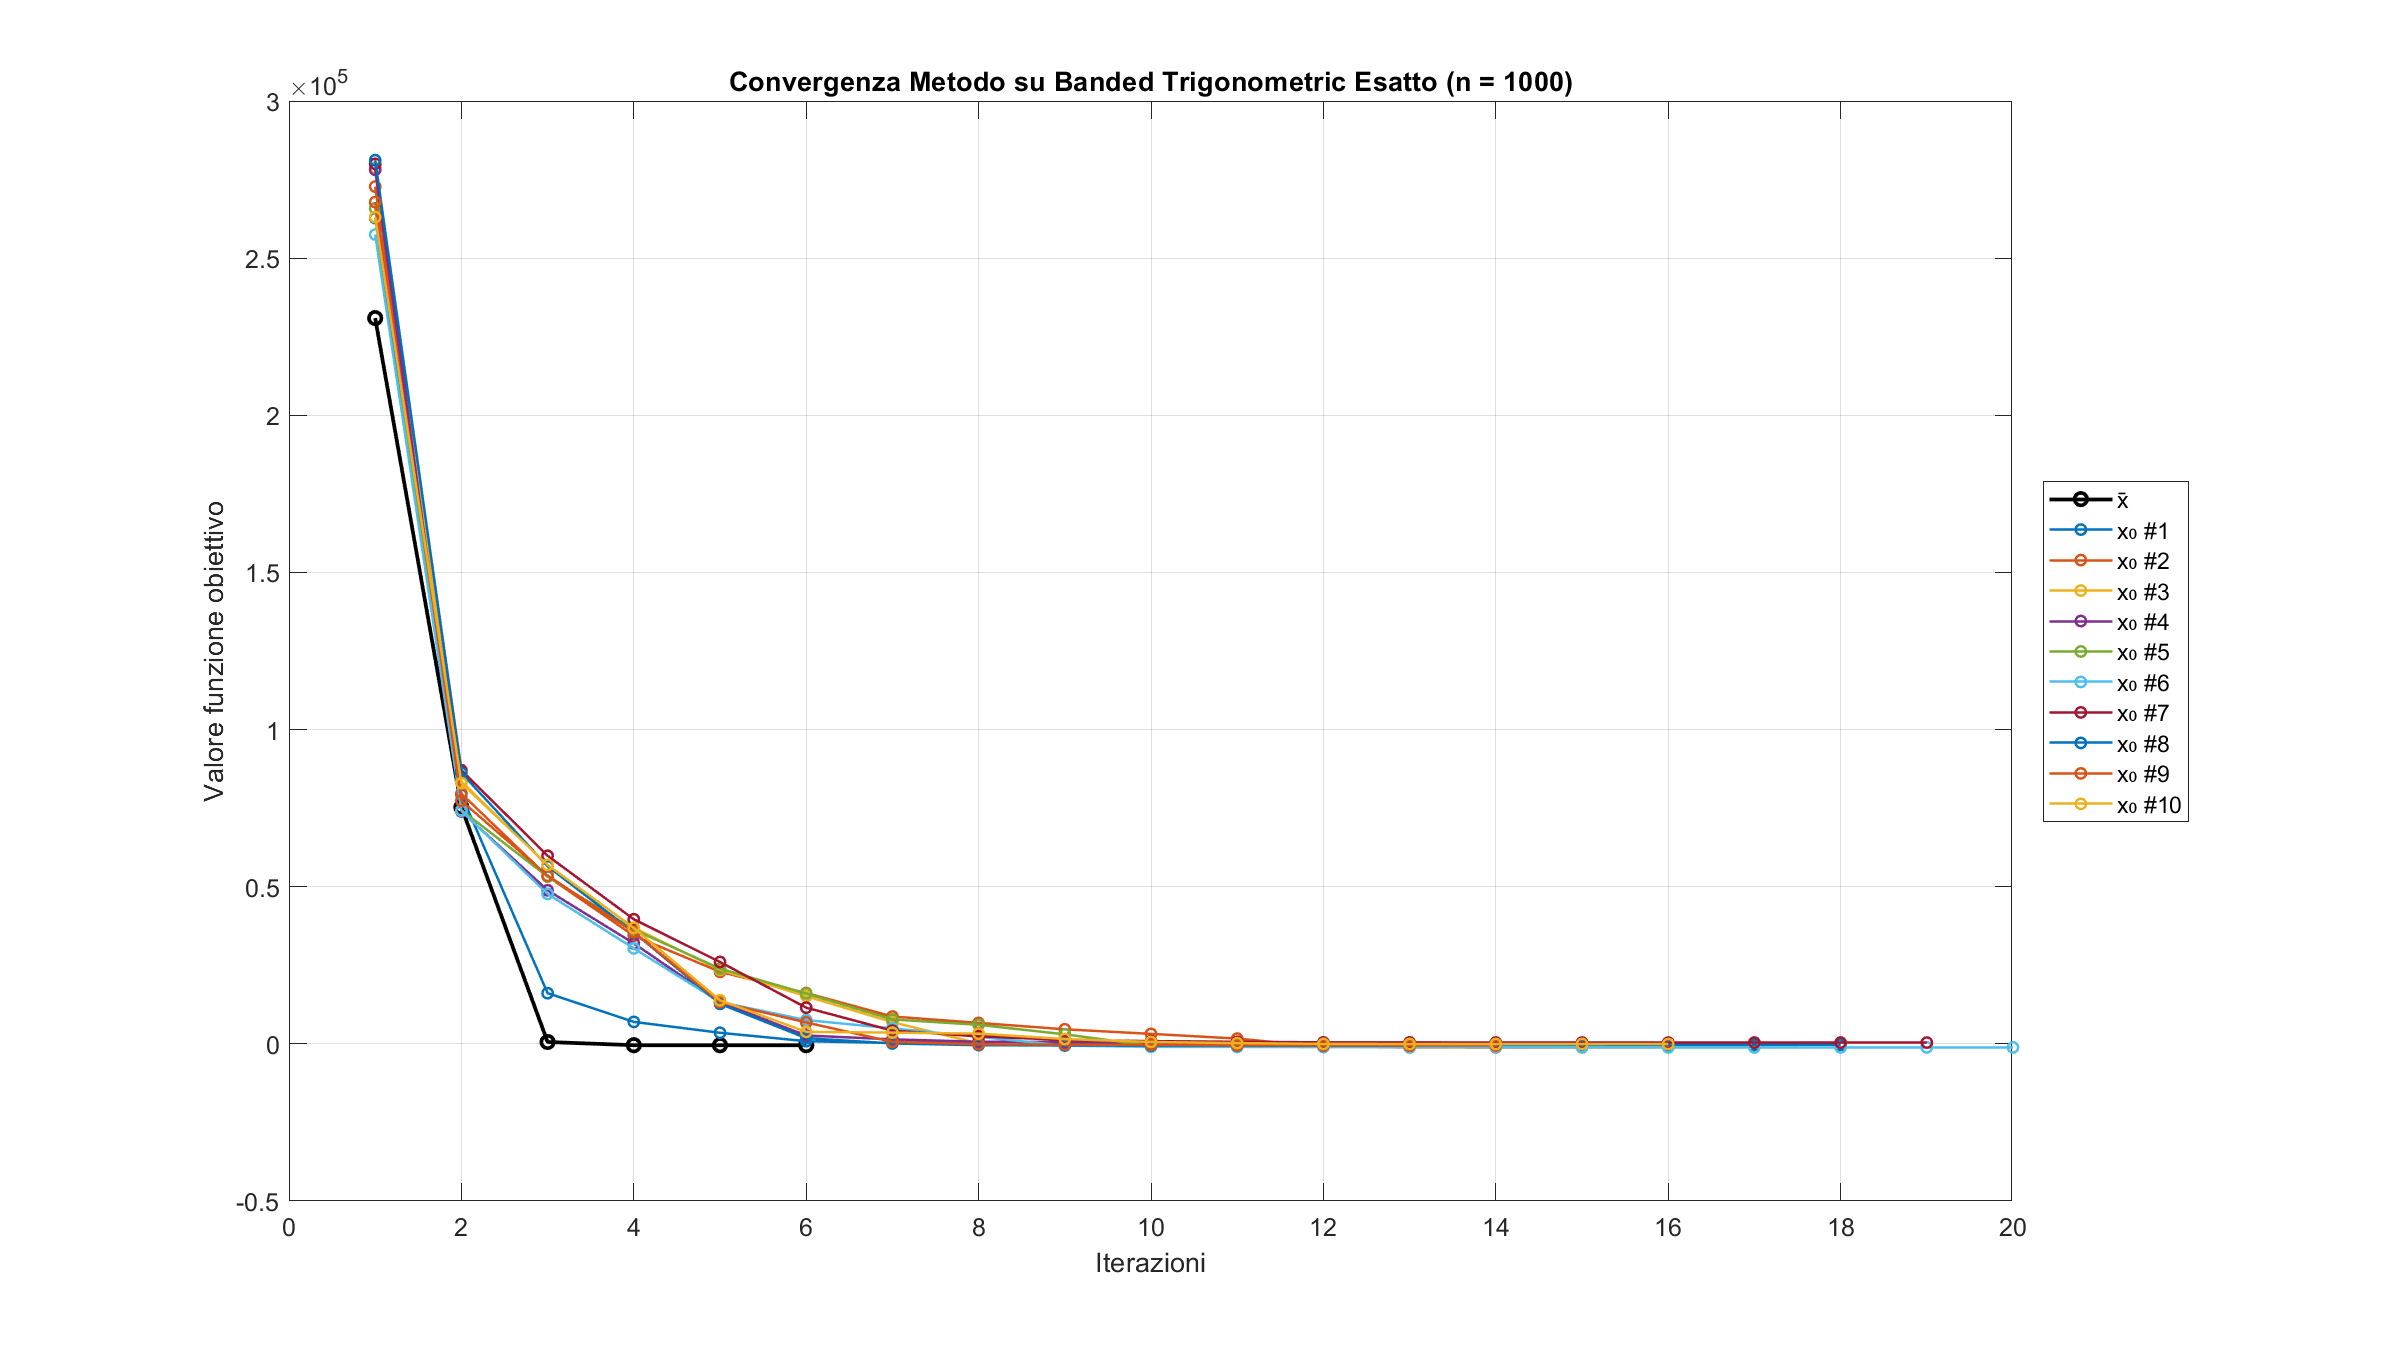
\includegraphics[width=\textwidth]{../immagini/banded_1k.png}
		\caption{Convergence of the Modified Newton method on the Banded Trigonometric function ($n=1000$) using exact derivatives.}
		\label{fig:bt_1k_exact}
	\end{figure}
	
	\begin{figure}[H]%[htbp]
		\centering
		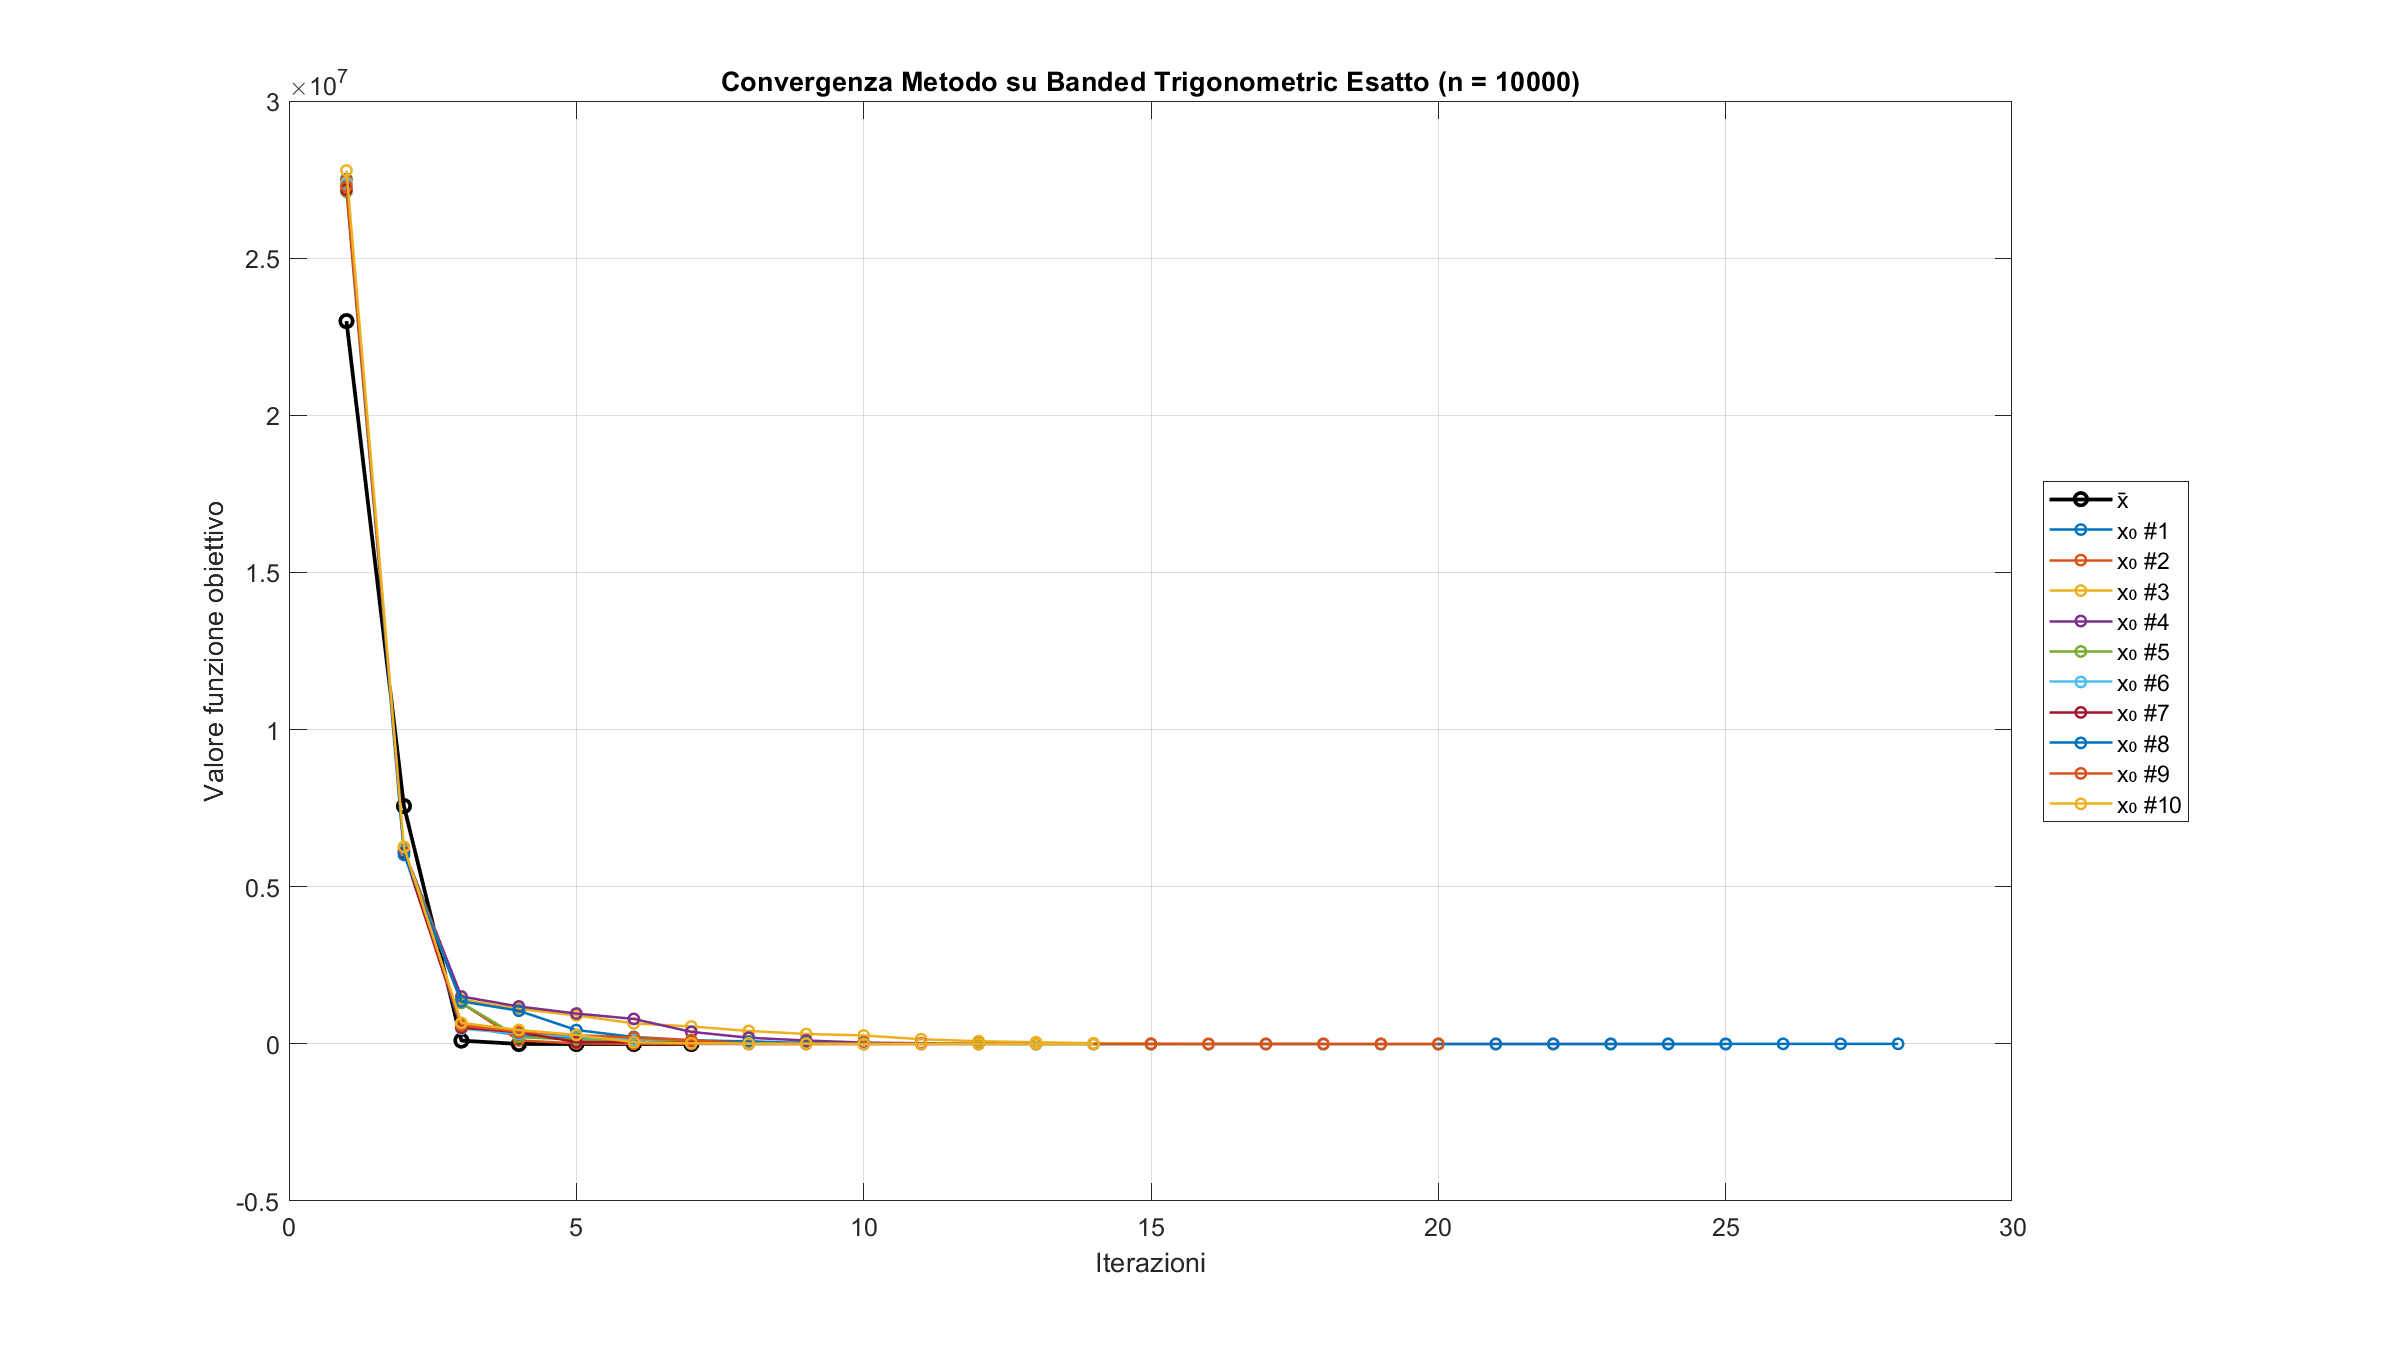
\includegraphics[width=\textwidth]{../immagini/banded_10k.png}
		\caption{Convergence of the Modified Newton method on the Banded Trigonometric function ($n=10000$) using exact derivatives.}
		\label{fig:bt_10k_exact}
	\end{figure}
	
	\begin{figure}[H]%[htbp]
		\centering
		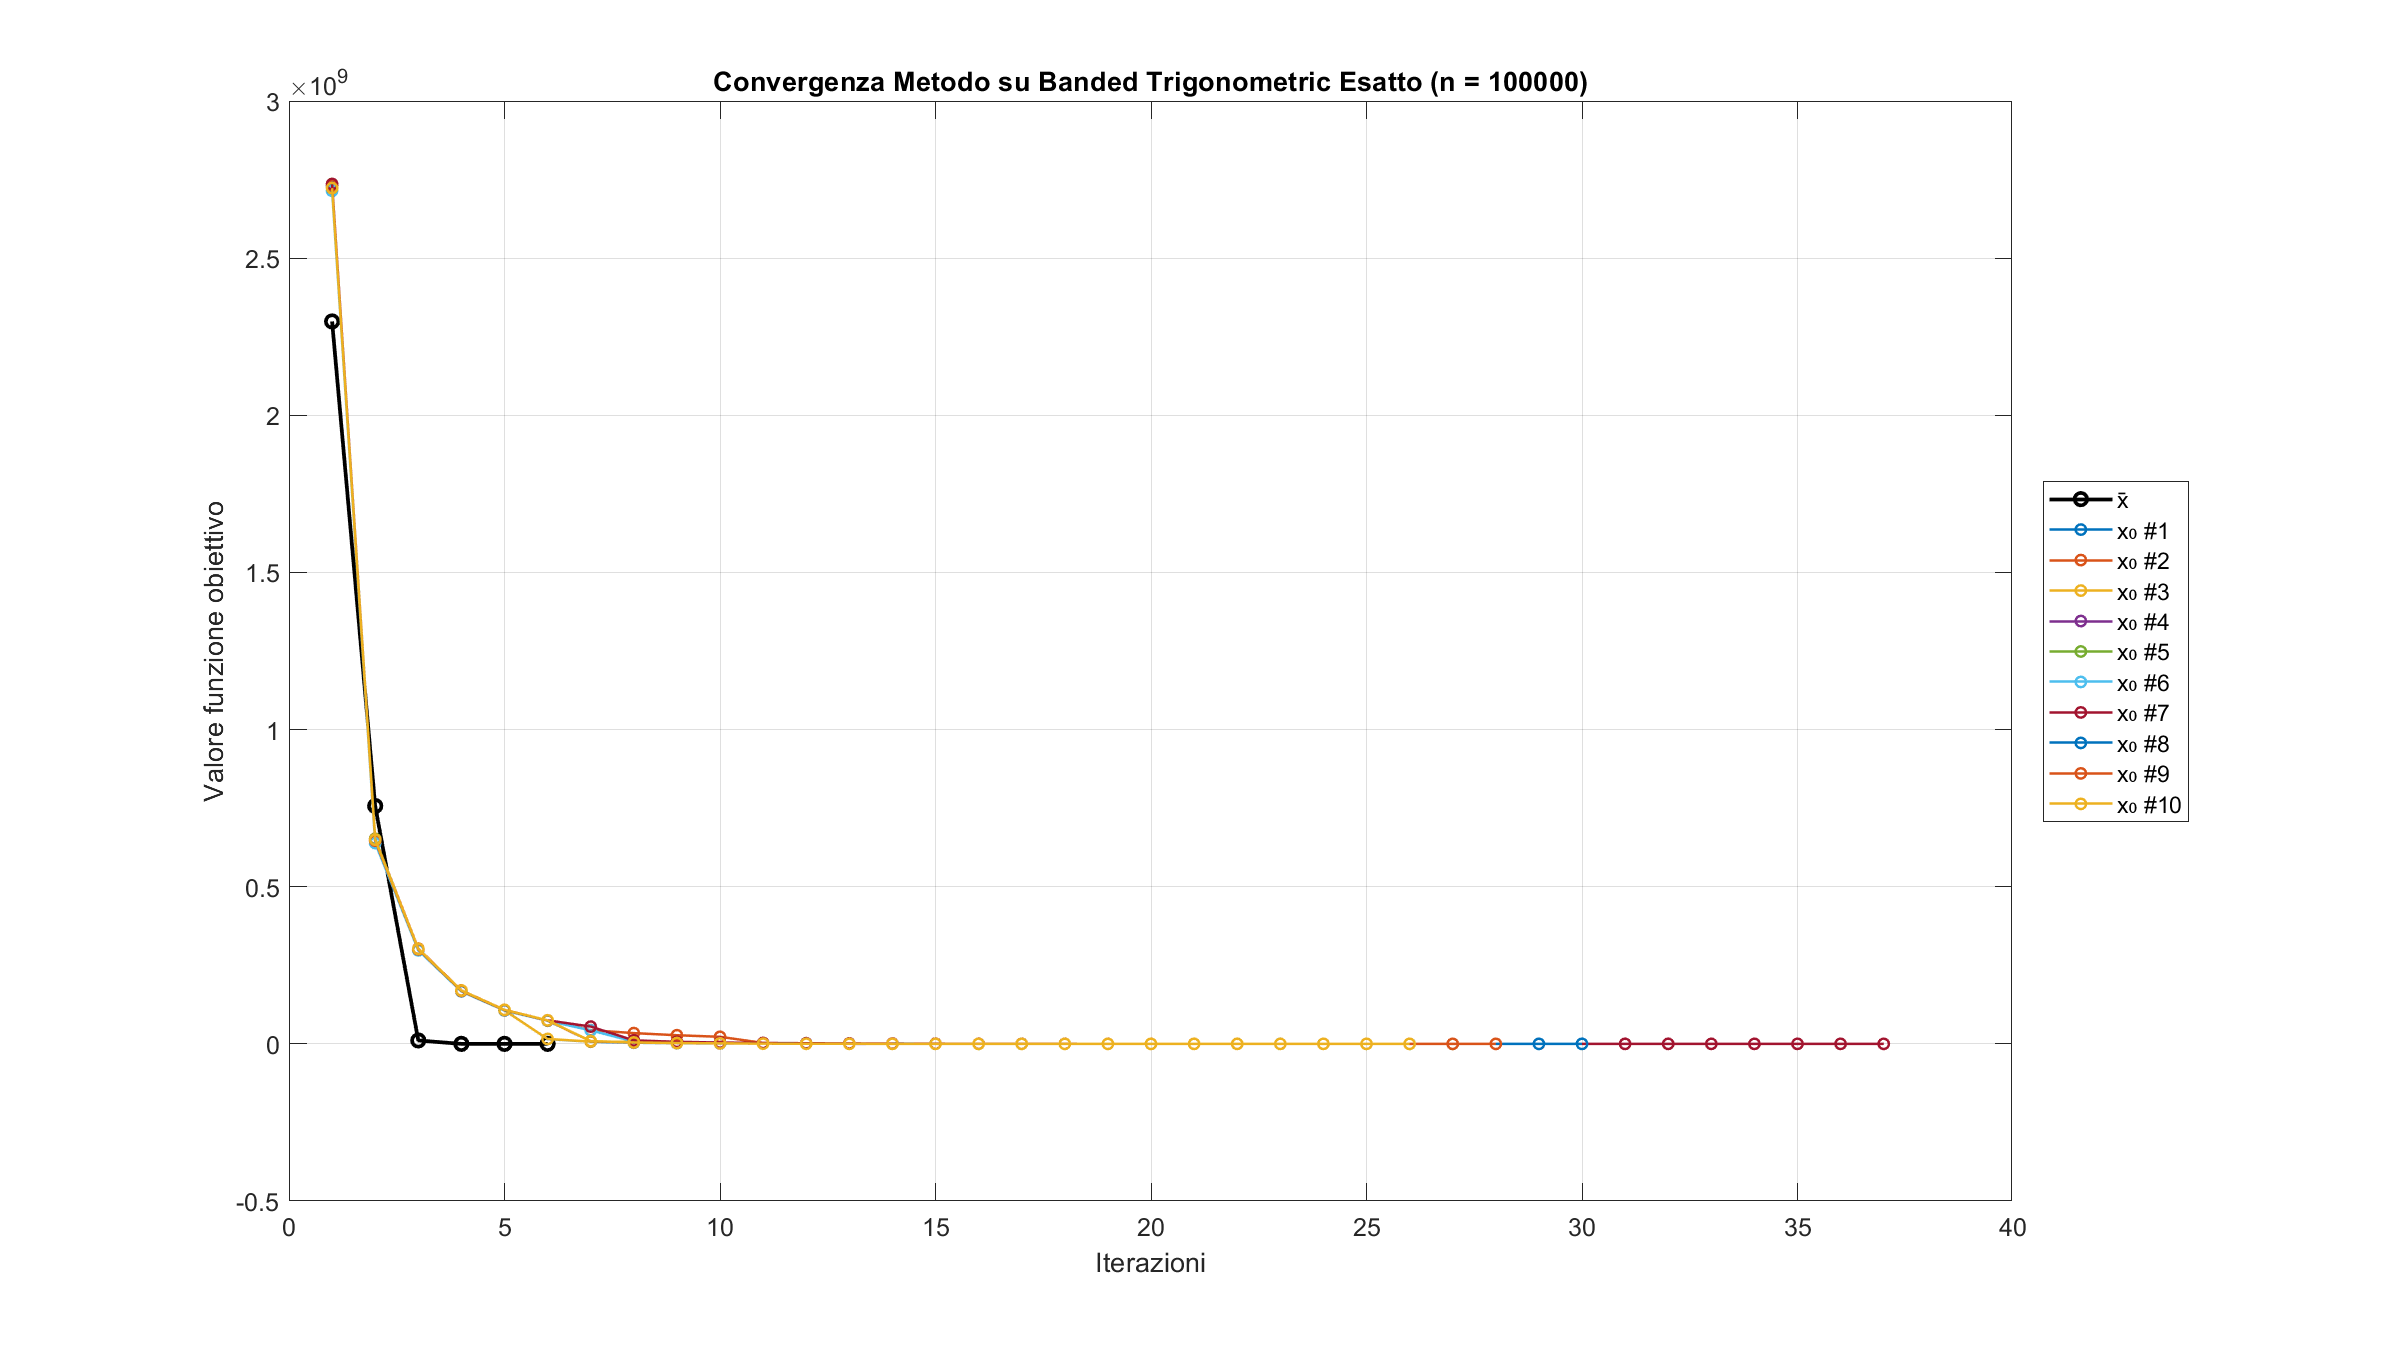
\includegraphics[width=\textwidth]{../immagini/banded_100k.png}
		\caption{Convergence of the Modified Newton method on the Banded Trigonometric function ($n=100000$) using exact derivatives.}
		\label{fig:bt_100k_exact}
	\end{figure}
	
	\begin{figure}[H]%[htbp]
		\centering
		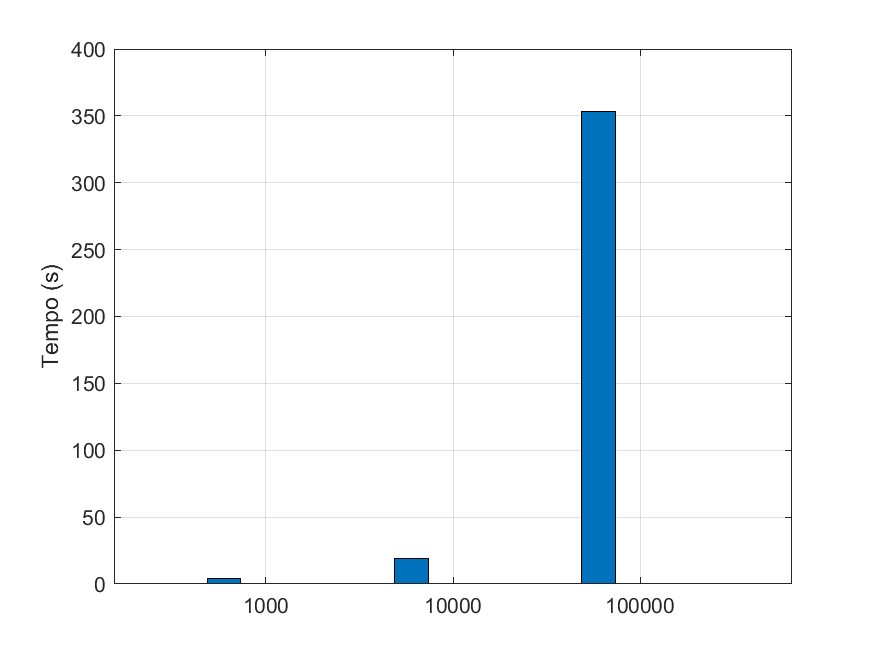
\includegraphics[width=0.55\textwidth]{../immagini/banded_time.png}
		\caption{Computational time required by the Modified Newton method on the Banded Trigonometric function with exact derivatives for each problem size.}
		\label{fig:bt_time_exact}
	\end{figure}
	
	\newpage
	

	\subsubsection{Modified Newton method with approximated derivatives}
	
	In this experiment, we use the Modified Newton method on the Banded Trigonometric function with gradient and hessian computed via finite differences. The approximated gradient and hessian components were expanded manually and implemented directly to avoid cancellation and redundancy. The sparsity pattern of the exact hessian was preserved to limit computational cost. The expressions used for approximating the gradient and the hessian are reported below, following the same structure adopted in previous sections.
	\paragraph{Gradient approximation.}
	Due to the structure of the function, only a small number of addends to the summation survive when computing the numerator in the formula (\ref{eq1}). These terms are identified by the following function: 
	\[
	g(x) = \sum_{i=k-1}^{k+1} i \left[ (1 - \cos(x_i)) + \sin(x_{i-1}) - \sin(x_{i+1}) \right].	
	\] 
	Then, using subtraction and addition formulas for sine and cosine, and fixed $k$ as the component whose derivative is being approximated:
	
	\begin{equation}
		\frac{\partial F}{\partial x_k} \approx \frac{g(x+he_{k}) - g(x+he_{k})}{2h} = \begin{cases}
			\frac{4 \cos x_k\sin h + 2k\sin x_k\sin h}{2h}, & 1 \leq k < n \\
			\frac{2n\sin x_n\sin h - 2(n-1) \cos x_k\sin h}{2h}, & k = n
		\end{cases}.
	\end{equation}
	
	\paragraph{Hessian approximation.}
	Also in the hessian computation, the definition of the function $g(x)$ can be used to describe the terms in the numerator of (\ref{eq3}). Rearranging the terms and using a Taylor expansion for the terms involving the cosine of h, is obtained:
	\begin{equation}
		\frac{\partial^2 F}{\partial x_k \partial x_j} \approx
		\begin{cases}
			(k \cos x_k - 2 \sin x_k) - h(k\sin x_k + 2 \cos x_k) , & 1 \leq k = j < n \\
			(n \cos x_n - (n-1) \sin x_n) - h(n\sin x_n -(n-1) \cos x_n), & k = j = n \\
			0, & \text{otherwise}
		\end{cases}.
	\end{equation}
	
	
	\vspace{1em}
	\newpage
	\paragraph{Experimental Results.}
	Also in this cas the Modified Newton method in unable to correctly optimize the Banded Trigonometric function. In all dimensions tested and for all starting points (suggested or randomly generated),  convergence is not met, and the algorithm stops after a few iterations regardless of whether the increment used in calculating finite differences is fixed or scaled by component. In this case it makes no sense to talk about the rate of convergence of the method implemented, in fact in some cases it cannot even be calculated (NaN). More precise results are captured in the following tables and figures, divided by problem size. 
	
	\newpage
	\begin{itemize}
		\item \boldmath $n = 1\,000$ \unboldmath
		\begin{table}[H]%[htbp]
		\centering
		\renewcommand{\arraystretch}{1.2}
		\resizebox{\textwidth}{!}{%
			\begin{tabular}{|c|c|c|c|c|c|}
				\hline
				\textbf{Increment} & \textbf{Init.} & \textbf{Iter} & \textbf{Time (s)} & \textbf{$\rho$} & \textbf{Successes} \\
				\hline
				$10^{-2}$ & $\bar{x}$ & 6 & 0.33 & 8.1635 & 1/1 \\
				$10^{-2}$ & Avg (10 pts) & 15.9 & 0.03 & 5.44 & 7/10 \\
				$10^{-2}\cdot|x|$ & $\bar{x}$ & 1 & 0.00 & NaN & 0/10 \\
				$10^{-2}\cdot|x|$ & Avg (10 pts) & 519 & 0.39 & 3.50 & 7/10 \\
				\hline
				$10^{-4}$ & $\bar{x}$ & 7 & 0.03 & 1.8294 & 0/1 \\
				$10^{-4}$ & Avg (10 pts) & 18.1 & 0.03 & 5.35 & 9/10 \\
				$10^{-4}\cdot|x|$ & $\bar{x}$ & 1 & 0.00 & NaN & 0/1 \\
				$10^{-4}\cdot|x|$ & Avg (10 pts) & 16.3 & 0.02 & 6.00 & 8/10 \\
				\hline
				$10^{-6}$ & $\bar{x}$ & 7 & 0.01 & 1.1623 & 1/1 \\
				$10^{-6}$ & Avg (10 pts) & 15.8 & 0.02 & 5.39 & 6/10 \\
				$10^{-6}\cdot|x|$ & $\bar{x}$ & 1 & 0.00 & NaN & 0/1 \\
				$10^{-6}\cdot|x|$ & Avg (10 pts) & 15.5 & 0.02 & 5.20 & 7/10 \\
				\hline
				$10^{-8}$ & $\bar{x}$ & 7 & 0.01 & 6.4828 & 1/1 \\
				$10^{-8}$ & Avg (10 pts) & 14.9 & 0.02 & 6.45 & 6/10 \\
				$10^{-8}\cdot|x|$ & $\bar{x}$ & 1 & 0.00 & NaN & 0/1 \\
				$10^{-8}\cdot|x|$ & Avg (10 pts) & 15 & 0.02 & 7.63 & 6/10 \\
				\hline
				$10^{-10}$ & $\bar{x}$ & 7 & 0.01 & 6.4832 & 1/1 \\
				$10^{-10}$ & Avg (10 pts) & 15.1 & 0.02 & 7.15 & 6/10 \\
				$10^{-10}\cdot|x|$ & $\bar{x}$ & 1 & 0.00 & NaN & 0/1 \\
				$10^{-10}\cdot|x|$ & Avg (10 pts) & 15.1 & 0.03 & 7.28 & 7/10 \\
				\hline
				$10^{-12}$ & $\bar{x}$ & 7 & 0.01 & 6.4832 & 1/1 \\
				$10^{-12}$ & Avg (10 pts) & 15.1 & 0.02 & 7.01 & 7/10 \\
				$10^{-12}\cdot|x|$ & $\bar{x}$ & 1 & 0.00 & NaN & 0/1 \\
				$10^{-12}\cdot|x|$ & Avg (10 pts) & 15.1 & 0.03 & 7.01 & 7/10 \\
				\hline
			\end{tabular}%
		}
		\label{tab:banded_fd_1000}
		\caption{Finite difference results for $n=1\,000$ using different increments $h$ and strategies.}
	\end{table}
	
	\newpage
	\begin{figure}[H]
		\centering
		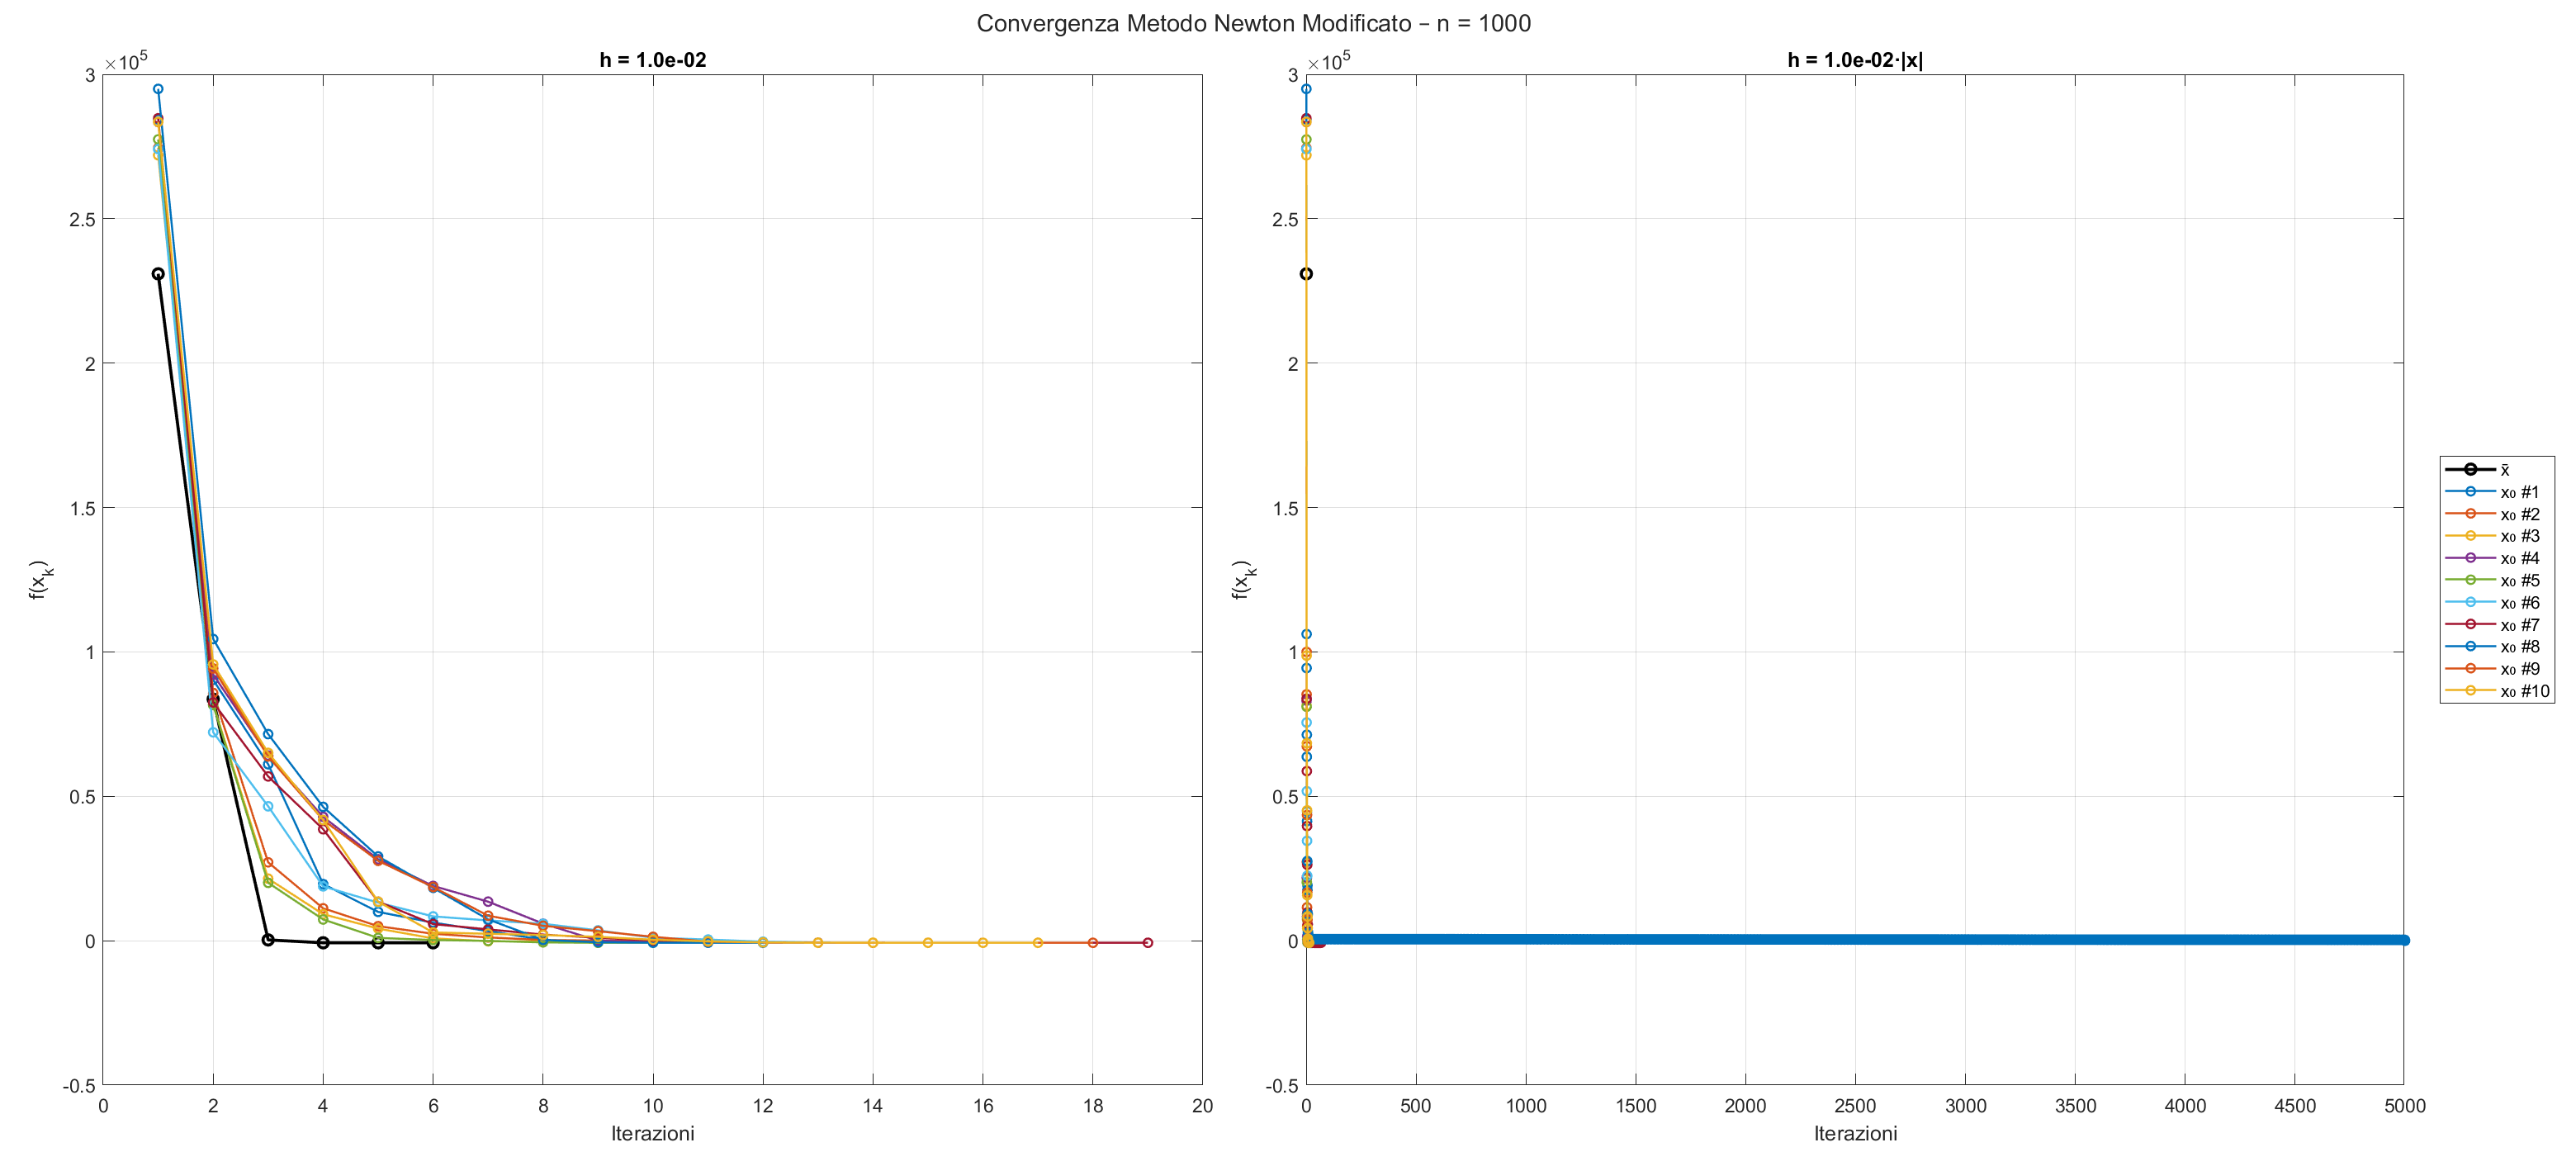
\includegraphics[width=\textwidth]{../immagini/banded_1k_h2.png}
		\caption{Convergence of the Modified Newton method on the Banded Trigonometric function ($n=1000$) using fixed increment $h = 10^{-2}$ (left) and scaled increment $h = 10^{-2}\cdot|x|$ (right).}
		\label{fig:bt_fd_1k_h2}
	\end{figure}
	
	\begin{figure}[H]%[htbp]
		\centering
		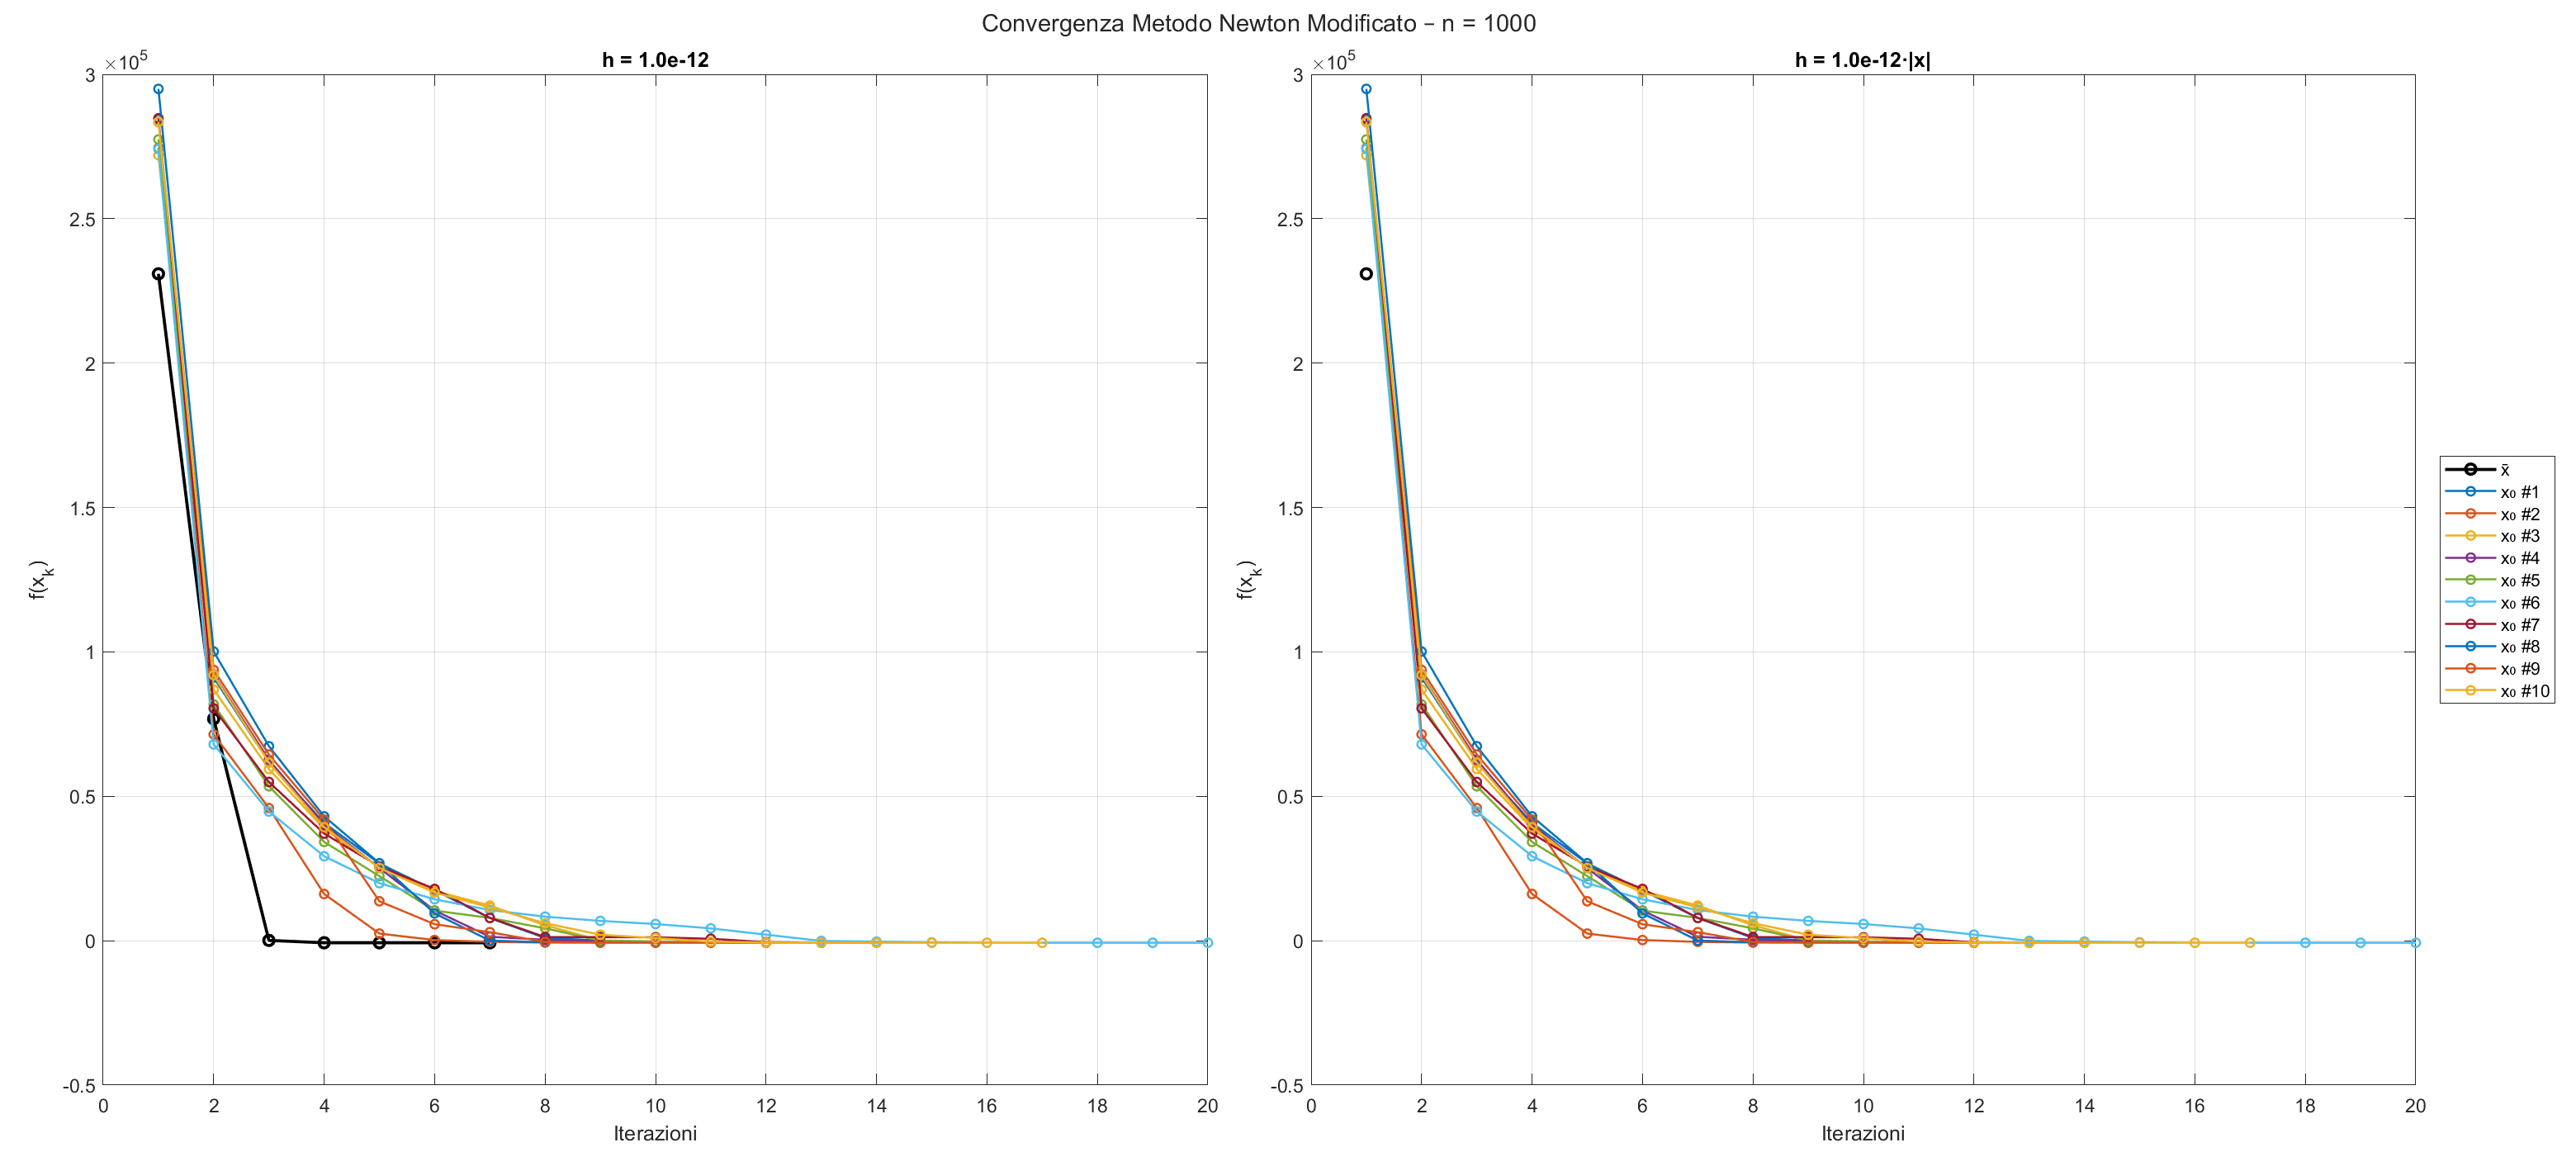
\includegraphics[width=\textwidth]{../immagini/banded_1k_h12.png}
		\caption{Convergence of the Modified Newton method on the Banded Trigonometric function ($n=1000$) using fixed increment $h = 10^{-12}$ (left) and scaled increment $h = 10^{-12}\cdot|x|$ (right).}
		\label{fig:bt_fd_1k_h12}
	\end{figure}
	\newpage
	
	\item \boldmath $n = 10\,000$ \unboldmath 
	\begin{table}[H]
		\centering
		\renewcommand{\arraystretch}{1.2}
		\resizebox{\textwidth}{!}{%
			\begin{tabular}{|c|c|c|c|c|c|}
				\hline
				\textbf{Increment} & \textbf{Init.} & \textbf{Iter} & \textbf{Time (s)} & \textbf{$\rho$} & \textbf{Successes} \\
				\hline
				$10^{-2}$ & $\bar{x}$ & 6 & 0.05 & -7087.89 & 1/1 \\
				$10^{-2}$ & Avg (10 pts) & 21.6 & 0.25 & 3.65 & 9/10 \\
				$10^{-2}\cdot|x|$ & $\bar{x}$ & 1 & 0.01 & NaN & 0/1 \\
				$10^{-2}\cdot|x|$ & Avg (10 pts) & 31.9 & 0.27 & 2.84 & 7/10 \\
				\hline
				$10^{-4}$ & $\bar{x}$ & 7 & 0.06 & 1.83 & 0/1 \\
				$10^{-4}$ & Avg (10 pts) & 20.8 & 0.24 & 6.73 & 8/10 \\
				$10^{-4}\cdot|x|$ & $\bar{x}$ & 1 & 0.01 & NaN & 0/1 \\
				$10^{-4}\cdot|x|$ & Avg (10 pts) & 20 & 0.23 & 5.13 & 8/10 \\
				\hline
				$10^{-6}$ & $\bar{x}$ & 7 & 0.06 & 1.16 & 1/1 \\
				$10^{-6}$ & Avg (10 pts) & 20.5 & 0.23 & 4.48 & 8/10 \\
				$10^{-6}\cdot|x|$ & $\bar{x}$ & 1 & 0.01 & NaN & 0/1 \\
				$10^{-6}\cdot|x|$ & Avg (10 pts) & 19.3 & 0.22 & 1.11 & 7/10 \\
				\hline
				$10^{-8}$ & $\bar{x}$ & 7 & 0.05 & 3.4828 & 1/1 \\
				$10^{-8}$ & Avg (10 pts) & 20.2 & 0.23 & 6.38 & 9/10 \\
				$10^{-8}\cdot|x|$ & $\bar{x}$ & 1 & 0.01 & NaN & 0/1 \\
				$10^{-8}\cdot|x|$ & Avg (10 pts) & 19.8 & 0.22 & 6.30 & 8/10 \\
				\hline
				$10^{-10}$ & $\bar{x}$ & 7 & 0.05 & 6.4832 & 1/1 \\
				$10^{-10}$ & Avg (10 pts) & 20.2 & 0.22 & 4.87 & 9/10 \\
				$10^{-10}\cdot|x|$ & $\bar{x}$ & 1 & 0.01 & NaN & 0/1 \\
				$10^{-10}\cdot|x|$ & Avg (10 pts) & 20.5 & 0.23 & 4.48 & 9/10 \\
				\hline
				$10^{-12}$ & $\bar{x}$ & 7 & 0.06 & 6.4832 & 1/1 \\
				$10^{-12}$ & Avg (10 pts) & 20.1 & 0.22 & 4.98 & 9/10 \\
				$10^{-12}\cdot|x|$ & $\bar{x}$ & 1 & 0.01 & NaN & 0/1 \\
				$10^{-12}\cdot|x|$ & Avg (10 pts) & 20.2 & 0.22 & 4.69 & 9/10 \\
				\hline
			\end{tabular}%
		}
		\label{tab:bt_fd_10000}
		\caption{Finite difference results for $n=10\,000$ using different increments $h$ and strategies.}
	\end{table}
	
	\newpage
	
	\begin{figure}[H]
		\centering
		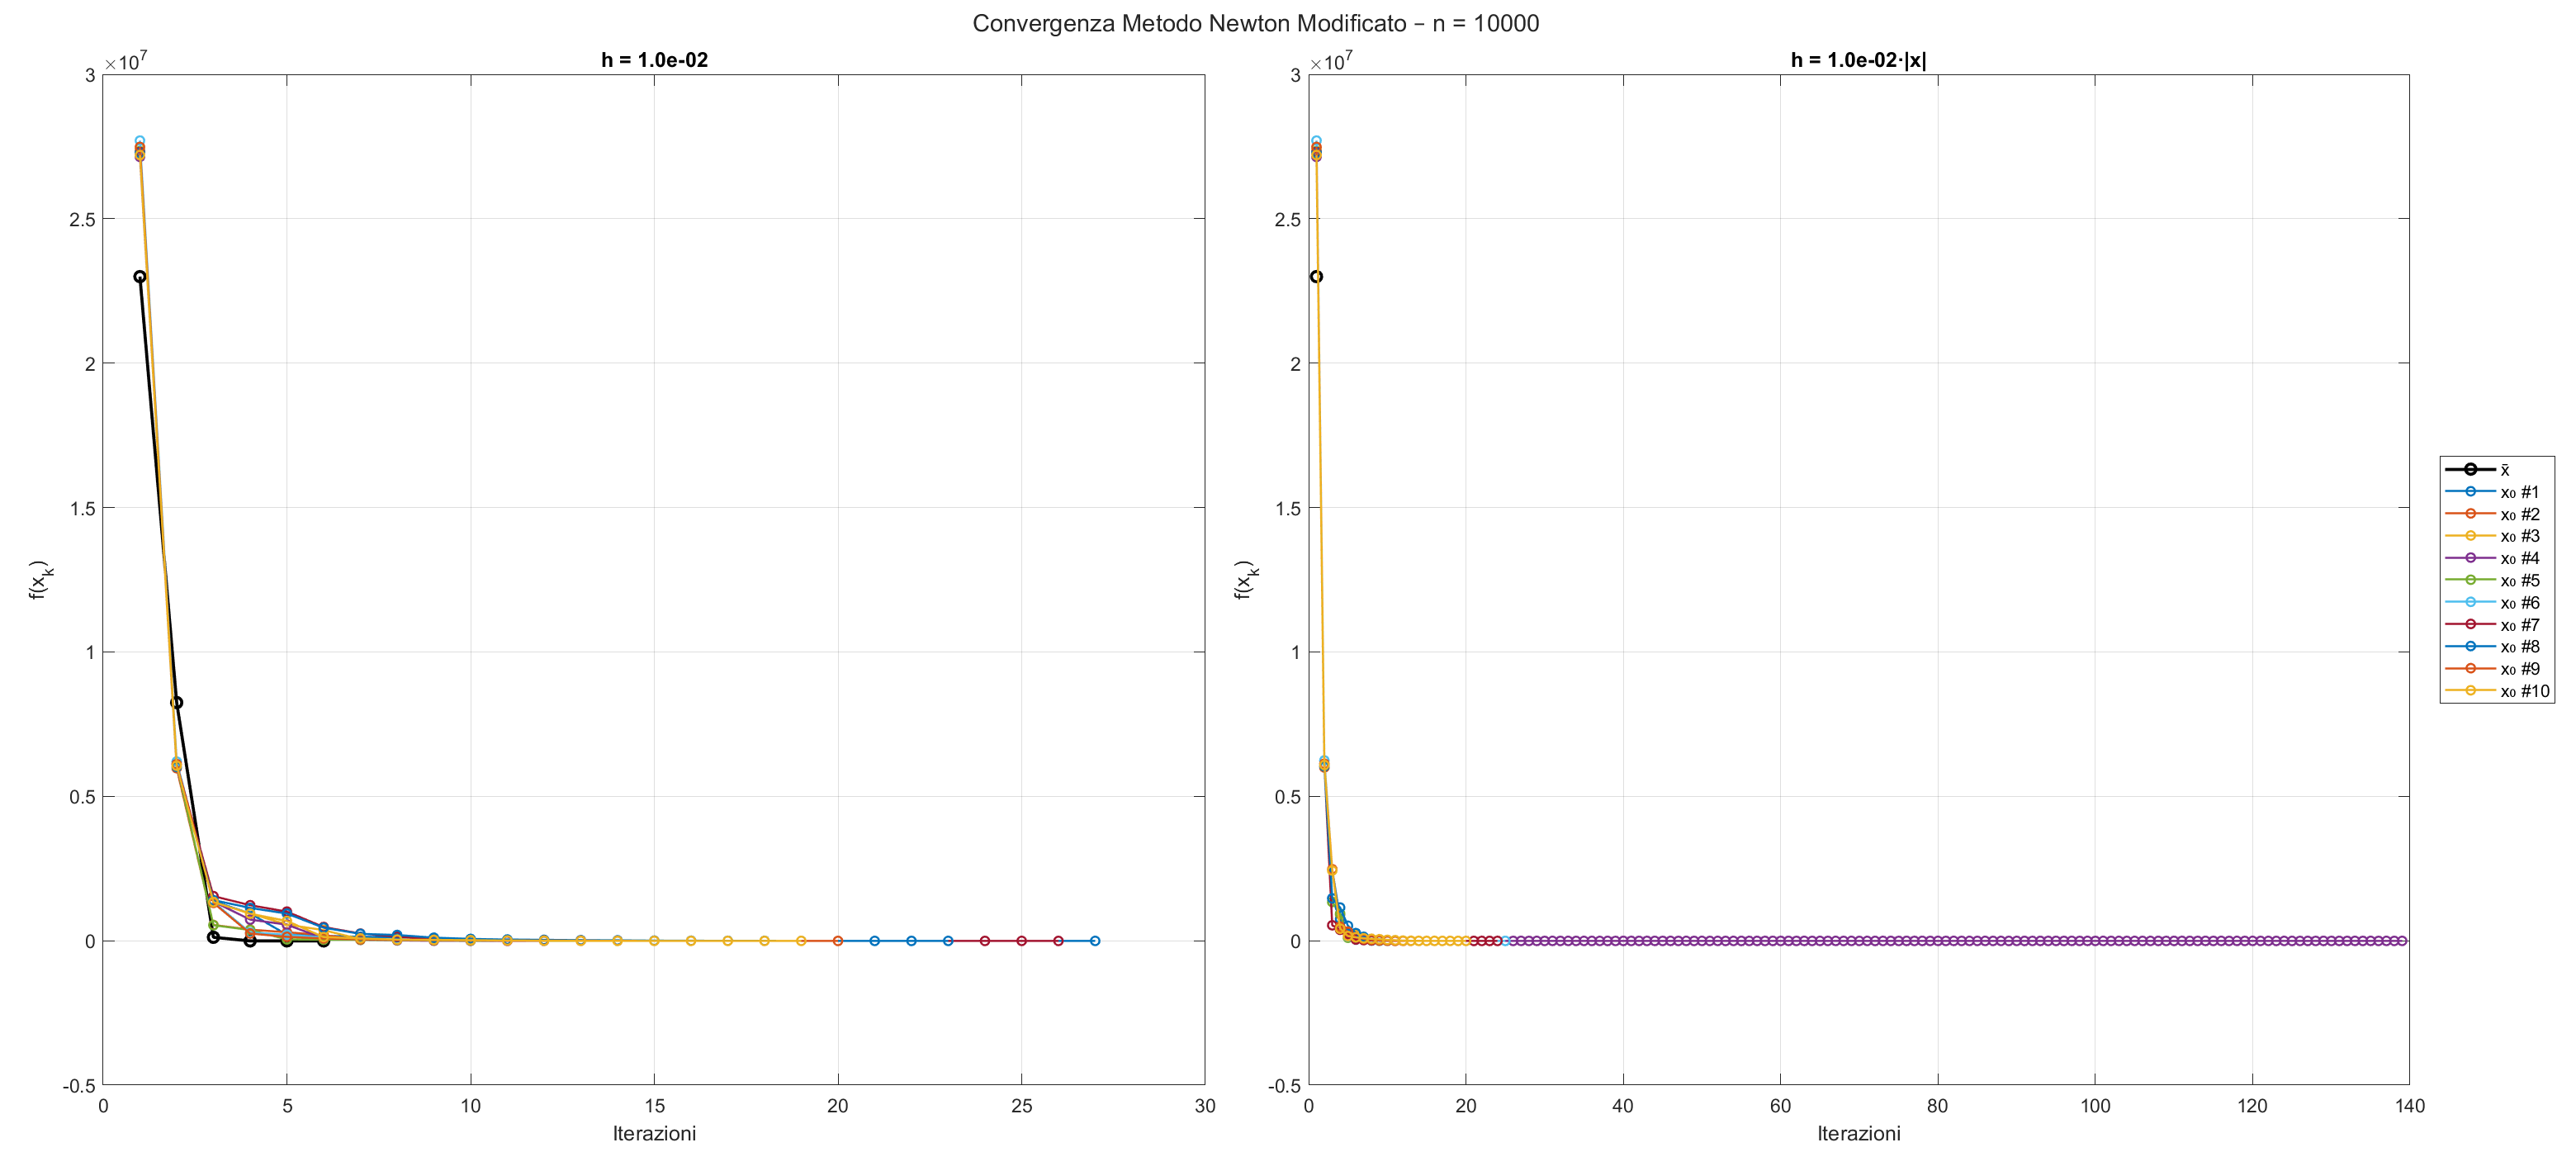
\includegraphics[width=\textwidth]{../immagini/banded_10k_h2.png}
		\caption{Convergence of the Modified Newton method on the Banded Trigonometric function ($n=10000$) using fixed increment $h = 10^{-2}$ (left) and scaled increment $h = 10^{-2}\cdot|x|$ (right).}
		\label{fig:bt_fd_10k_h2}
	\end{figure}
	
	\begin{figure}[H]%[htbp]
		\centering
		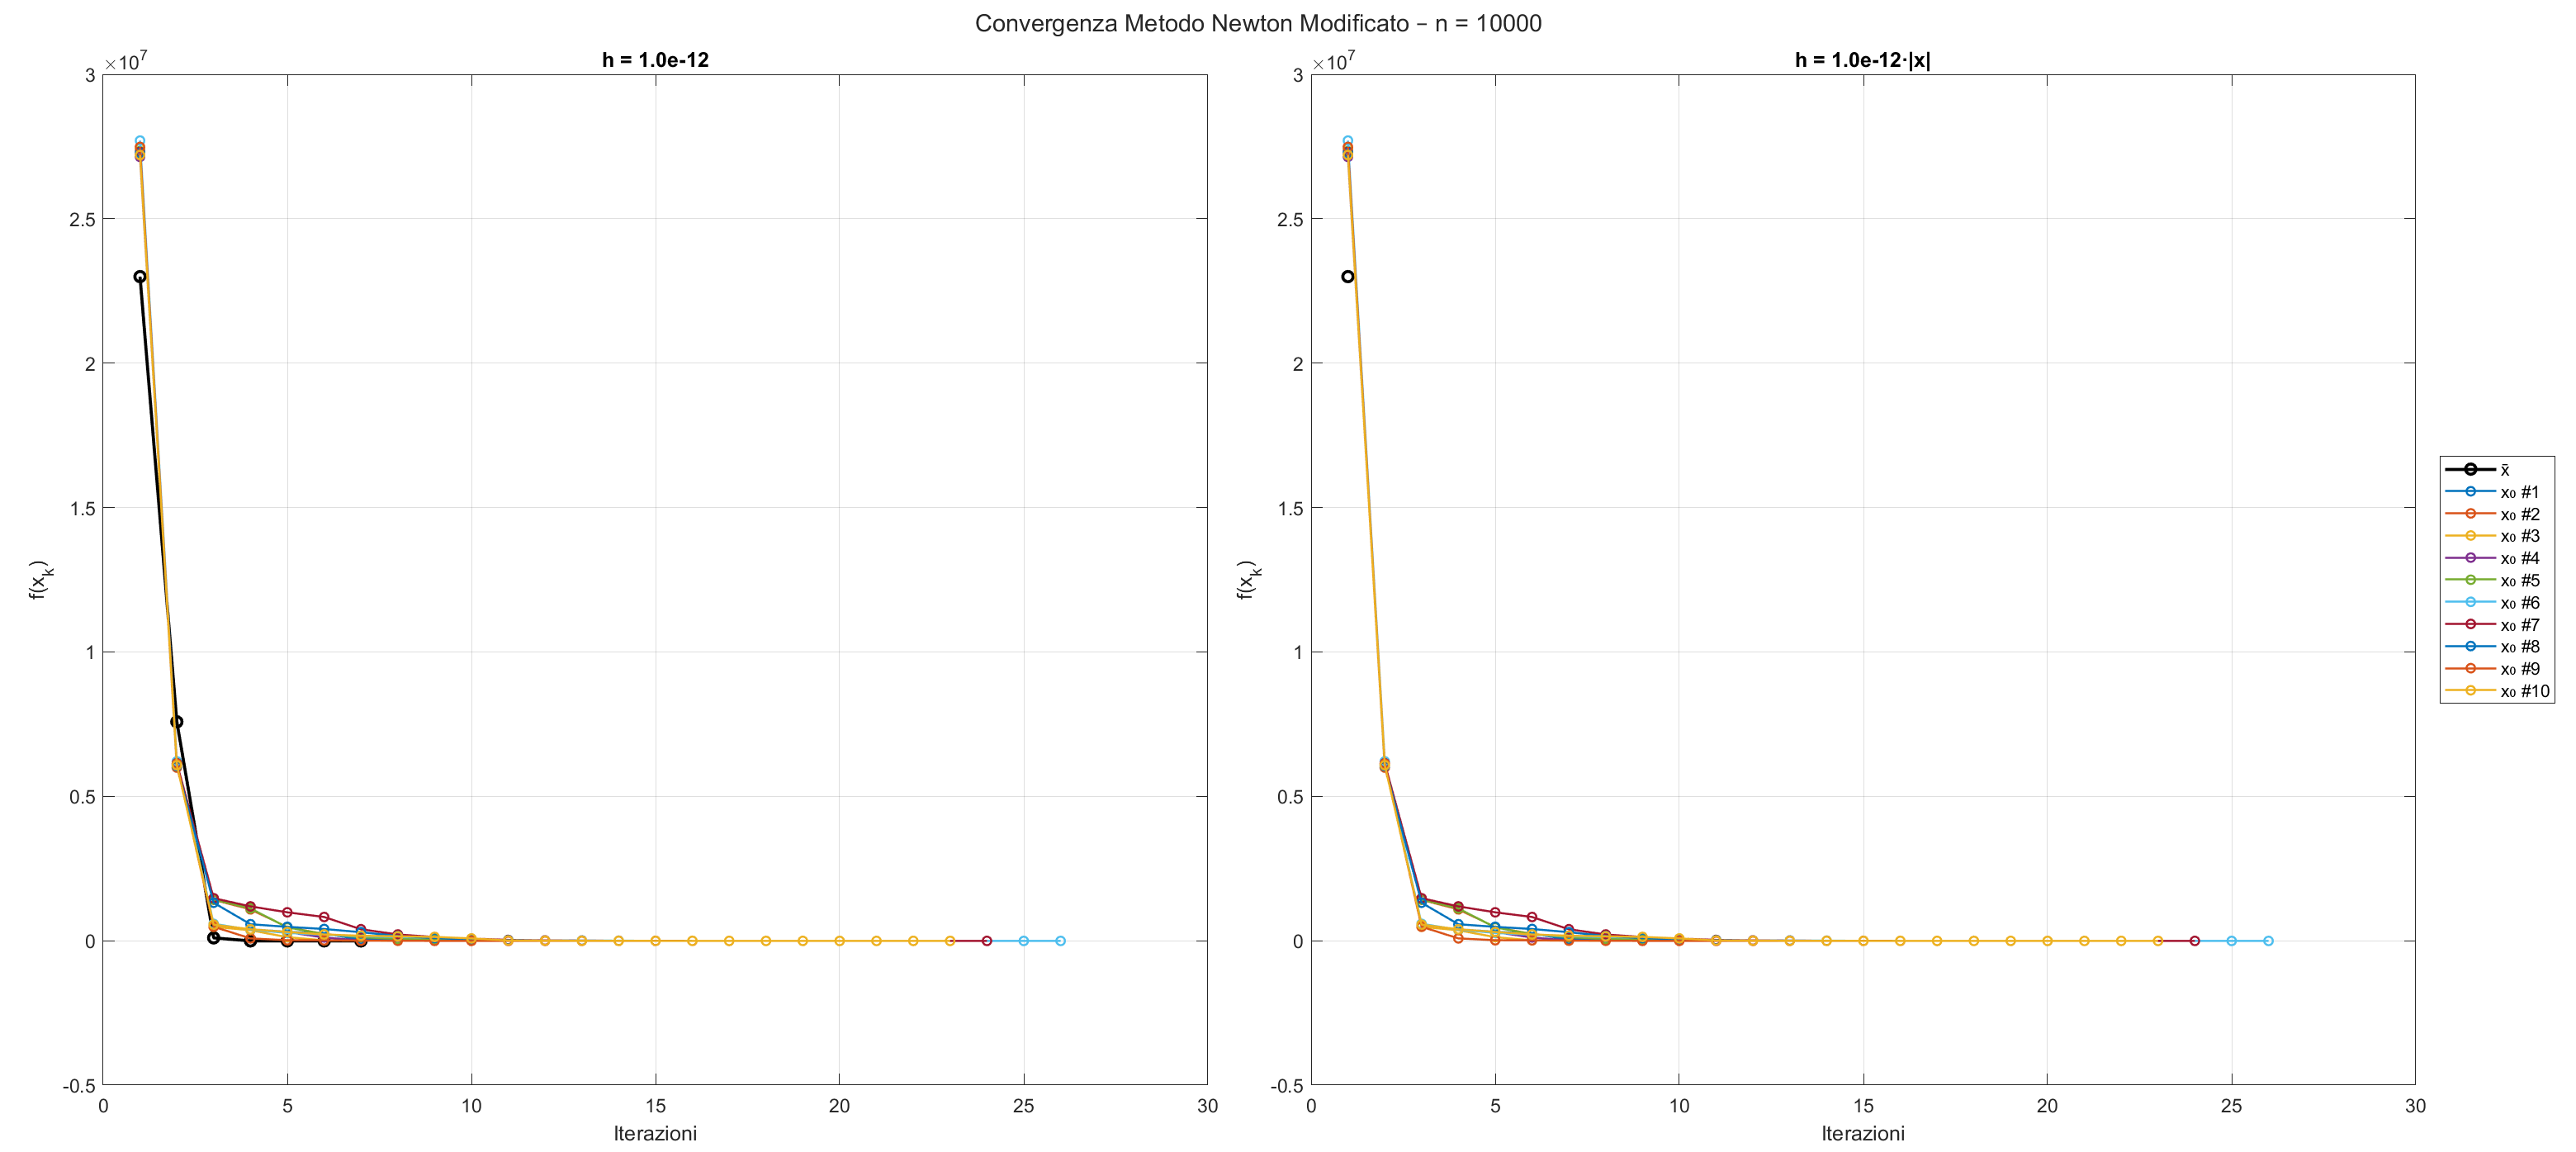
\includegraphics[width=\textwidth]{../immagini/banded_10k_h12.png}
		\caption{Convergence of the Modified Newton method on the Banded Trigonometric function ($n=10000$) using fixed increment $h = 10^{-12}$ (left) and scaled increment $h = 10^{-12}\cdot|x|$ (right).}
		\label{fig:bt_fd_10k_h12}
	\end{figure}
	
	
	
	\newpage
	
	\item \boldmath $n = 100\,000$ \unboldmath
	\begin{table}[H]
		\centering
		\renewcommand{\arraystretch}{1.2}
		\resizebox{\textwidth}{!}{%
			\begin{tabular}{|c|c|c|c|c|c|}
				\hline
				\textbf{Increment} & \textbf{Init.} & \textbf{Iter} & \textbf{Time (s)} & \textbf{$\rho$} & \textbf{Successes} \\
				\hline
				$10^{-2}$ & $\bar{x}$ & 6 & 0.37 & 8.1604 & 1/1 \\
				$10^{-2}$ & Avg (10 pts) & 29.3 & 4.59 & 6.36 & 8/10 \\
				$10^{-2}\cdot|x|$ & $\bar{x}$ & 1 & 0.09 & NaN & 0/1 \\
				$10^{-2}\cdot|x|$ & Avg (10 pts) & 41.3 & 7.00 & 4.22 & 8/10 \\
				\hline
				$10^{-4}$ & $\bar{x}$ & 7 & 0.50 & 1.8294 & 0/1 \\
				$10^{-4}$ & Avg (10 pts) & 28.4 & 4.61 & 4.51 & 8/10 \\
				$10^{-4}\cdot|x|$ & $\bar{x}$ & 1 & 0.09 & NaN & 0/1 \\
				$10^{-4}\cdot|x|$ & Avg (10 pts) & 29 & 4.59 & 5.31 & 8/10 \\
				\hline
				$10^{-6}$ & $\bar{x}$ & 7 & 0.50 & 1.1623 & 1/1 \\
				$10^{-6}$ & Avg (10 pts) & 28.9 & 4.92 & 6.26 & 8/10 \\
				$10^{-6}\cdot|x|$ & $\bar{x}$ & 1 & 0.09 & NaN & 0/1 \\
				$10^{-6}\cdot|x|$ & Avg (10 pts) & 28.6 & 4.72 & 8.31 & 7/10 \\
				\hline
				$10^{-8}$ & $\bar{x}$ & 7 & 0.58 & 6.4828 & 1/1 \\
				$10^{-8}$ & Avg (10 pts) & 29.6 & 4.70 & 4.01 & 8/10 \\
				$10^{-8}\cdot|x|$ & $\bar{x}$ & 1 & 0.09 & NaN & 0/1 \\
				$10^{-8}\cdot|x|$ & Avg (10 pts) & 30.8 & 5.19 & 6.75 & 8/10 \\
				\hline
				$10^{-10}$ & $\bar{x}$ & 7 & 0.53 & 6.4832 & 1/1 \\
				$10^{-10}$ & Avg (10 pts) & 28 & 4.43 & 5.83 & 9/10 \\
				$10^{-10}\cdot|x|$ & $\bar{x}$ & 1 & 0.09 & NaN & 0/1 \\
				$10^{-10}\cdot|x|$ & Avg (10 pts) & 31.1 & 4.95 & 2.63 & 9/10 \\
				\hline
				$10^{-12}$ & $\bar{x}$ & 7 & 0.51 & 6.4832 & 1/1 \\
				$10^{-12}$ & Avg (10 pts) & 29.8 & 4.83 & 0.88 & 8/10 \\
				$10^{-12}\cdot|x|$ & $\bar{x}$ & 1 & 0.09 & NaN & 0/1 \\
				$10^{-12}\cdot|x|$ & Avg (10 pts) & 30.9 & 4.86 & 4.18 & 8/10 \\
				\hline
			\end{tabular}%
		}
		\label{tab:banded_fd_100000}
		\caption{Finite difference results for $n=100\,000$ using different increments $h$ and strategies.}
		
	\end{table}
	\newpage
	\begin{figure}[H]
		\centering
		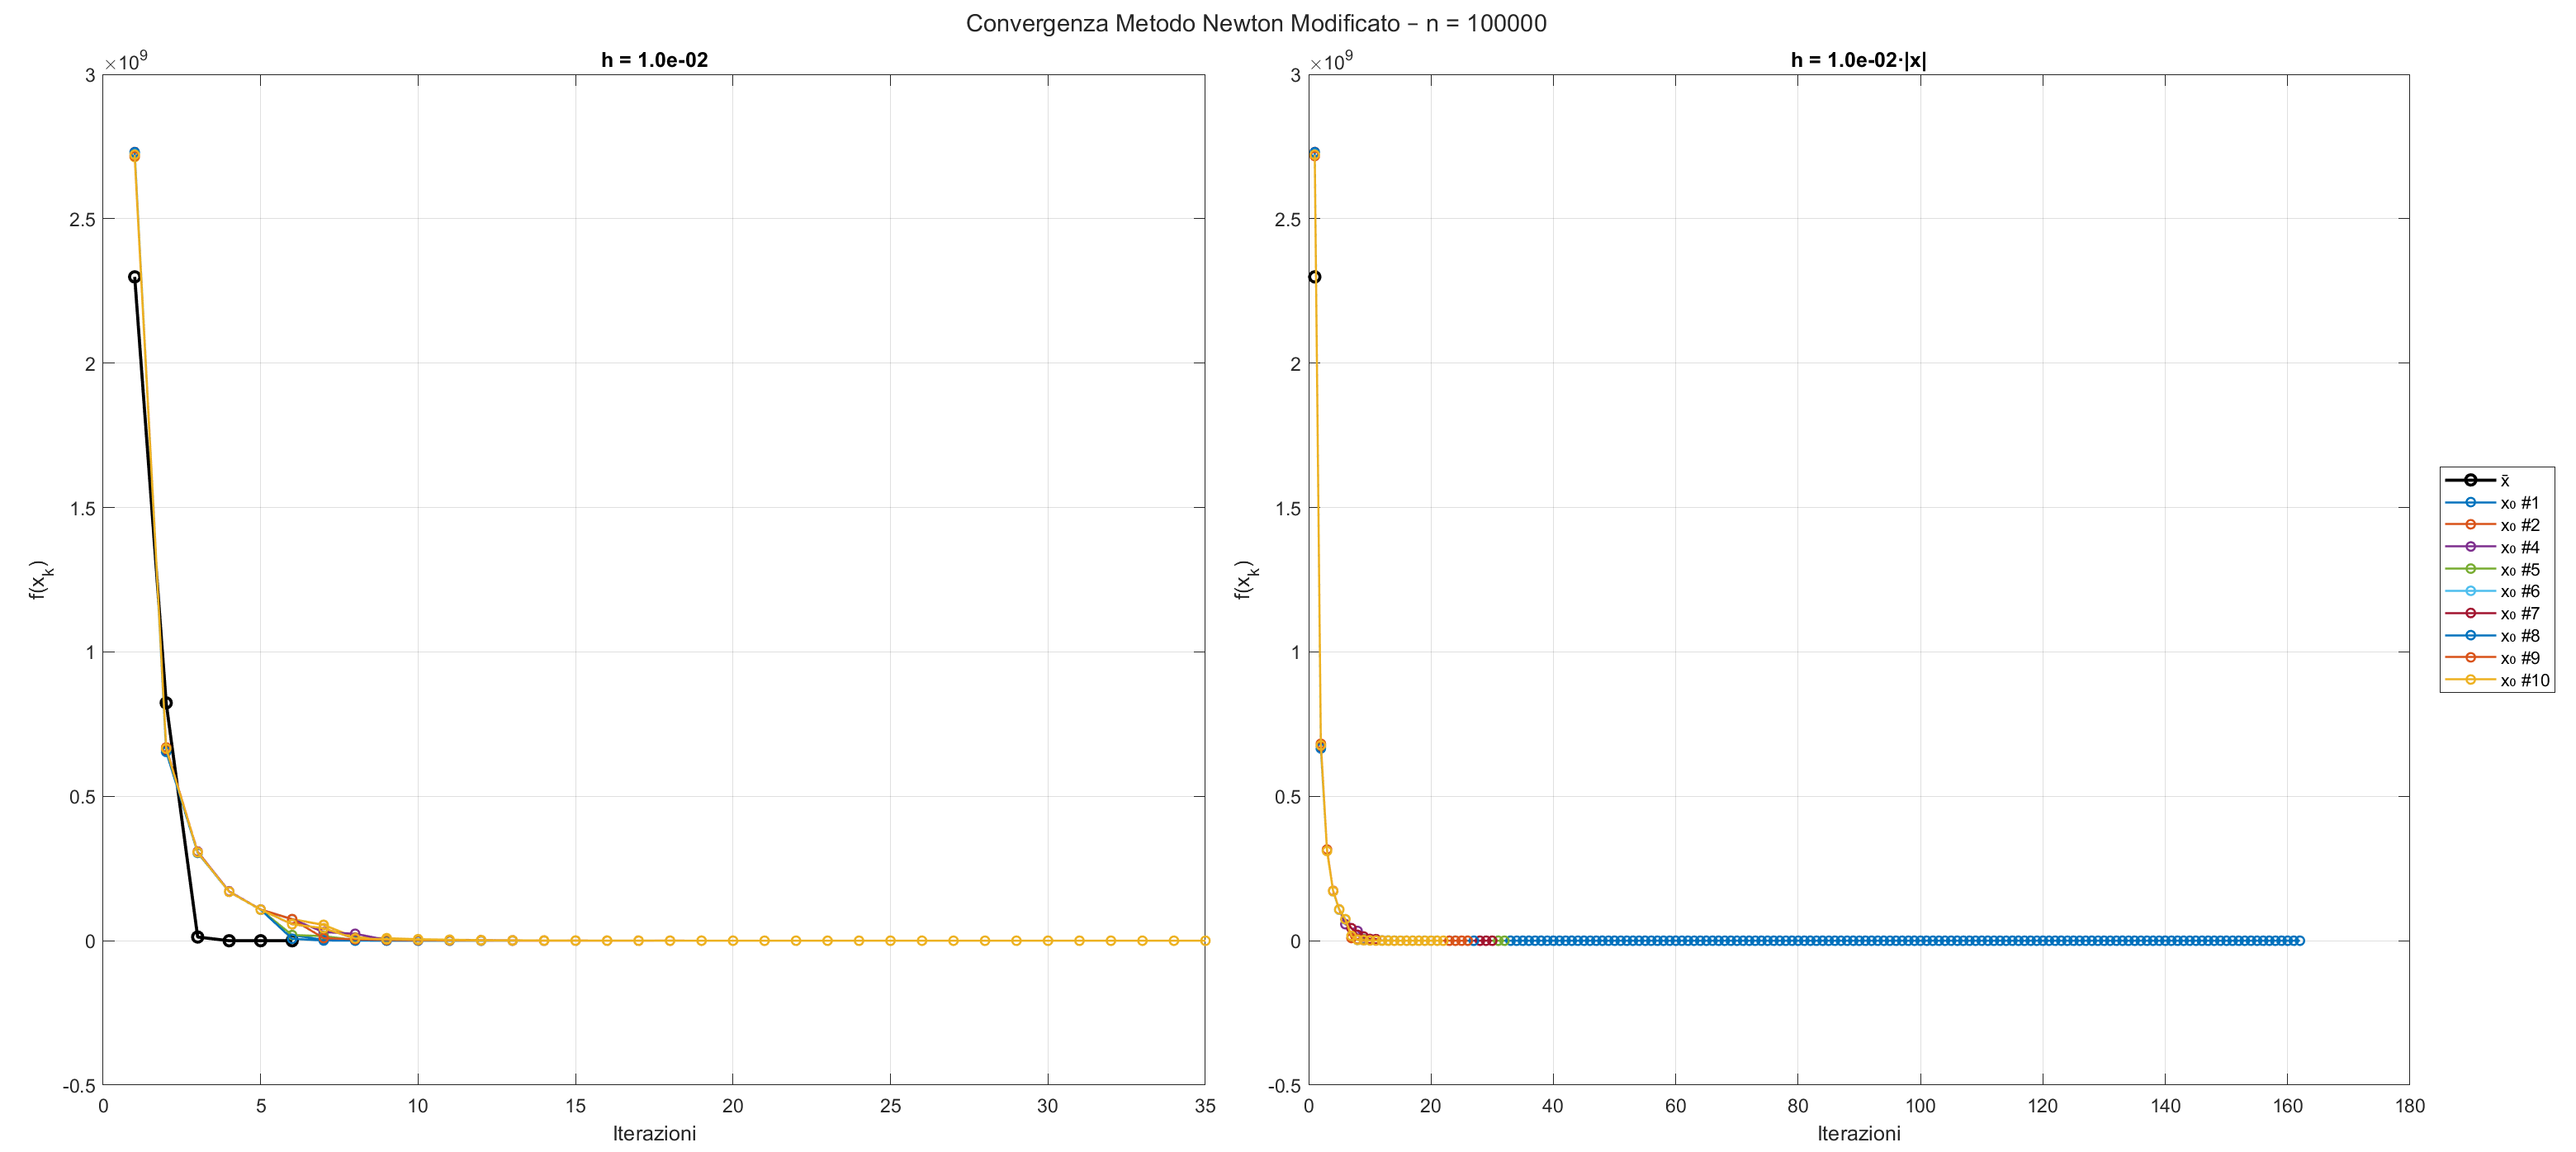
\includegraphics[width=\textwidth]{../immagini/banded_100k_h2.png}
		\caption{Convergence of the Modified Newton method on the Banded Trigonometric function ($n=100000$) using fixed increment $h = 10^{-2}$ (left) and scaled increment $h = 10^{-2}\cdot|x|$ (right).}
		\label{fig:bt_fd_100k_h2}
	\end{figure}
	
	\begin{figure}[H]%[htbp]
		\centering
		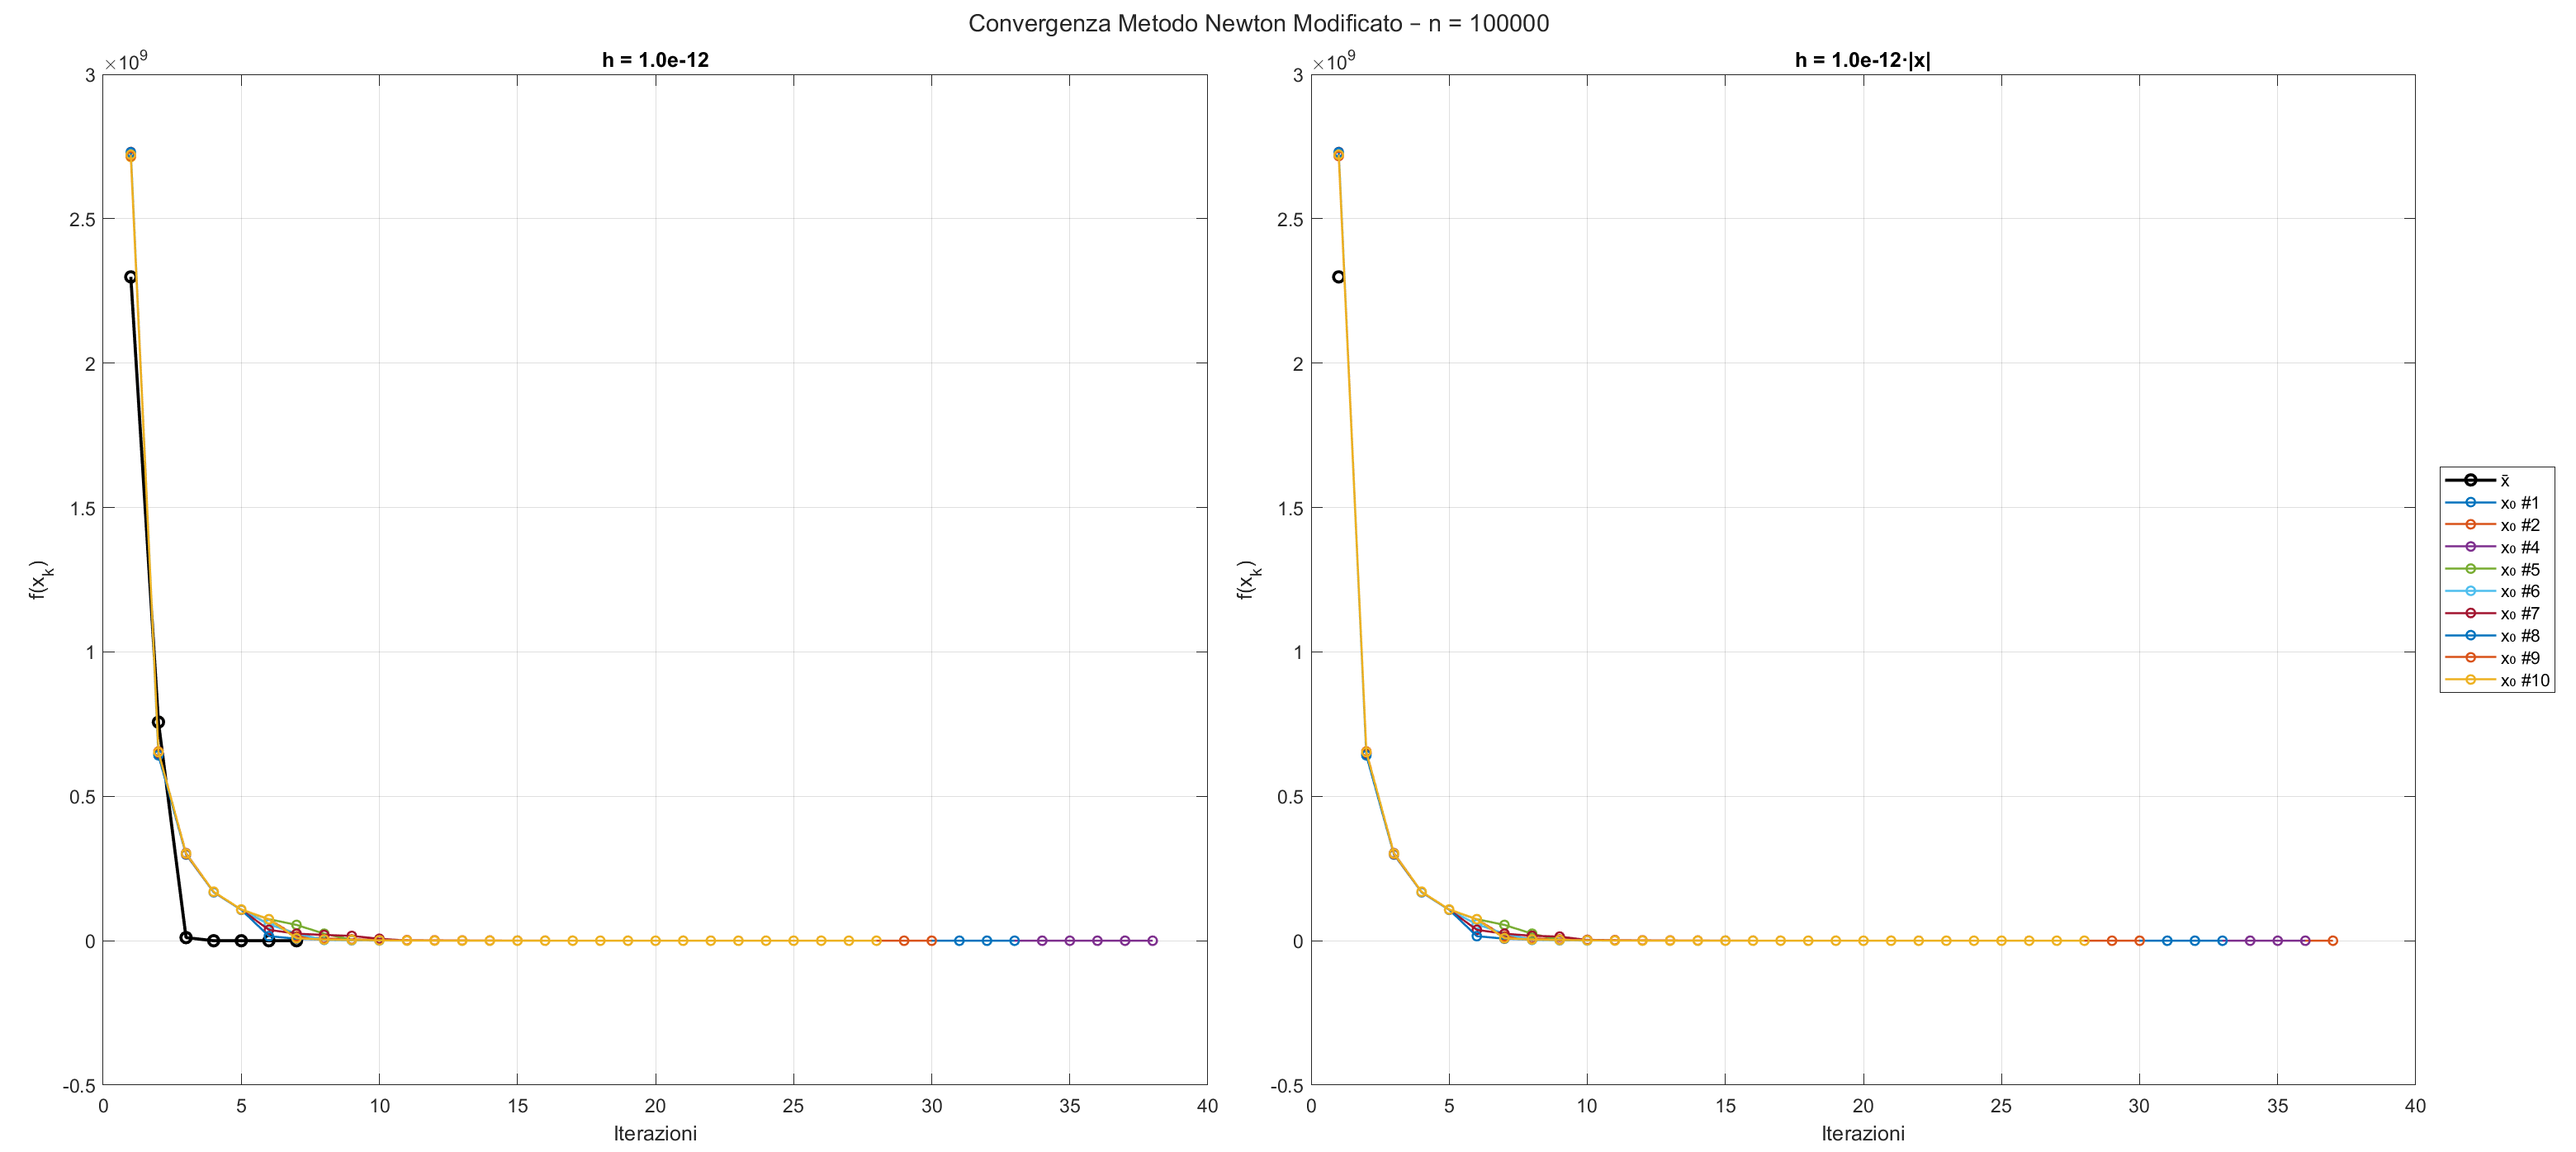
\includegraphics[width=\textwidth]{../immagini/banded_100k_h12.png}
		\caption{Convergence of the Modified Newton method on the Banded Trigonometric function ($n=100000$) using fixed increment $h = 10^{-12}$ (left) and scaled increment $h = 10^{-12}\cdot|x|$ (right).}
		\label{fig:bt_fd_100k_h12}
	\end{figure}
	
\end{itemize}

	\newpage
	\subsection{Nelder–Mead method}
	In this subsection are shown the results obtained from the minimization of the Banded Trigonometric function using the Nelder--Mead method. This method does not exploit derivative information and therefore struggles more with ill-conditioned landscapes and high-dimensional domains. As expected, the performance worsens as the dimension increases.\\
	
	\noindent Before presenting the results, a general experimental setup is given:
	\begin{itemize}
		\item \texttt{n} $= 10, 26, 50$;
		\item \texttt{max\_iter} $= 100.000$
		\item \texttt{tol} $= 10^{-6}$.
	\end{itemize}
	%	\vspace{0.5cm}
	
	Moreover, for each run have been recorded:
	\begin{itemize}
		\item number of iterations to convergence;
		\item CPU time;
		\item final objective value found \(f_{min}\);
		\item experimental rate of convergence \(\rho\):
		\[
		\rho \approx \frac{\log\left(\|x^{(k+1)} - x^{(k)}\|\big/\|x^{(k)} - x^{(k-1)}\|\right)}{\log\left(\|x^{(k)} - x^{(k-1)}\|\big/\|x^{(k-1)} - x^{(k-2)}\|\right)}.
		\]
			\end{itemize}
	
	In correspondence with the randomly generated points, an average behavior of each of the previous catogories is reported.
		
	\vspace{1em}
	\paragraph{Experimental results.}
	The experimental results for the Banded Trigonometric function confirm the limitations of the Nelder–Mead method in high-dimensional and structured nonlinear problems. For $n=10$, the method achieves very low computational times and iteration counts, but only 2 out of 10 runs with random initializations are successful, and function values remain distant from the global minimum in most cases. As the dimension increases to $n=26$ and $n=50$, the number of iterations and total computational time increase drastically, with several runs hitting the iteration cap (notably, two runs at $n=26$ required 80000 iterations and over 50 seconds). No successful runs are observed for these higher dimensions, and the convergence rates $\rho$ become highly erratic, alternating between extreme positive and negative values, indicating a lack of stability and robustness. Overall, the method fails to provide accurate or reliable solutions in medium and high dimensions, reinforcing the need for derivative-based or more advanced global optimization methods when tackling large-scale, structured, and highly nonlinear problems.
	
	
	\begin{table}[H]
		\renewcommand{\arraystretch}{1.2}
		\resizebox{\textwidth}{!}{%
			\begin{tabular}{|c|c|c|c|c|c|}
				\hline
				\textbf{Dimension} & \textbf{Starting point} & \textbf{$f_{\min}$} & \textbf{Iter} & \textbf{Time (s)} & \textbf{$\rho$} \\
				\hline
				10  & $\bar{x}$         & -2.180187   & 187    & 0.01  & 0.5000  \\
				& Avg (10 pts)      & -9.743851   & 1297   & 0.019 & 0.5390  \\
				\hline
				26  & $\bar{x}$         & -6.731719   & 1376   & 0.04  & -7.0805 \\
				& Avg (10 pts)      & 2.086111    & 77855  & 6.393 & 4.1805  \\
				\hline
				50  & $\bar{x}$         & -5.995540   & 4955   & 0.28  & -1.8208 \\
				& Avg (10 pts)      & -2.092789   & 65323  & 0.429 & 0.1752  \\
				\hline
			\end{tabular}%
		}
		\caption{Results of Nelder–Mead on Banded Trigonometric function.}
		\label{tab:nelder_bandedtrig}
	\end{table}
	
	\newpage
	\begin{figure}[H]
		\centering
		\includegraphics[width=\textwidth]{../immagini/banded_10.png}
		\caption{Convergence of Nelder-Mead on the Banded Trigonometric function with $n = 10$.}
		\label{fig:bt_nelder_10}
	\end{figure}
	
	\begin{figure}[htbp]
		\centering
		\includegraphics[width=\textwidth]{../immagini/banded_26.png}
		\caption{Convergence of Nelder-Mead on the Banded Trigonometric function with $n = 26$.}
		\label{fig:bt_nelder_26}
	\end{figure}
	
	\begin{figure}[htbp]
		\centering
		\includegraphics[width=\textwidth]{../immagini/banded_50.png}
		\caption{Convergence of Nelder-Mead on the Banded Trigonometric function with $n = 50$.}
		\label{fig:bt_nelder_50}
	\end{figure}
	
	\begin{figure}[htbp]
		\centering
		\includegraphics[width=0.6\textwidth]{../immagini/banded_time_nelder.png}
		\caption{Computation time of Nelder-Mead on the Banded Trigonometric function for $n \in \{10, 26, 50\}$.}
		\label{fig:bt_nelder_time}
	\end{figure}
		
	
	\section{Conclusions}
	
	In this project, we implemented and compared the performance of two numerical optimization methods—Modified Newton and Nelder–Mead—on three benchmark unconstrained problems:
	\begin{enumerate}
	\item Extended Rosenbrock function,
	\item Generalized Broyden Tridiagonal function,
	\item Banded Trigonometric function.
	\end{enumerate}
	
	The Modified Newton method consistently delivered superior results across all tested functions and dimensions. When exact derivatives were available, the method achieved rapid convergence—often in fewer than 10 iterations—and scaled efficiently even in high-dimensional settings (e.g. $n = 10^5$), thanks to sparse linear algebra and preconditioning techniques. Finite difference approximations, although more computationally expensive and slightly less accurate, proved to be reliable when properly tuned, particularly with smaller step sizes (e.g. $h \leq 10^{-6}$).\\
	
	In contrast, the Nelder–Mead method showed acceptable performance only in low-dimensional cases. While easy to implement and free of derivative requirements, its convergence became erratic and inefficient as the dimension increased. The algorithm often failed to reach low objective values, especially in problems with ill-conditioned or structured landscapes, such as the Banded Trigonometric function.\\
	
	Overall, this study highlights the importance of leveraging second-order information and exploiting problem structure—such as sparsity or tridiagonality—for scalable and reliable optimization. Derivative-free methods may still be useful in small-scale or noisy settings, but for large, structured problems, Newton-type algorithms remain the preferred choice.
	
	% -------------------------------------------------
	\newpage
	\appendix
	\section*{Appendix: MATLAB Codes}
	\addcontentsline{toc}{section}{Appendix: MATLAB Codes}
	
	In this appendix we report the commented MATLAB scripts and functions developed for the assignment. All codes are provided with inline comments to clarify each computational step and choice. The file and function names correspond to those used in the computational experiments described in the main text.
	
	\subsection*{Modified Newton Method on Rosenbrock function 2D}
	\addcontentsline{toc}{subsection}{Modified Newton Method on Rosenbrock function 2D}
	
	\begin{lstlisting}[language=Matlab,caption={Modified Newton Method with Armijo Backtracking Line Search},label={lst:modified-newton}]
		function [x_min, f_min, iter, min_history] = modified_newton(f, grad_f, hess_f, x0, tol, max_iter,name)
		% Implementation of Modified Newton Method with Armijo Backtracking Line Search
		
		% Inputs:
		%   f: Function handle of the objective function
		%   grad_f: Function handle of the gradient
		%   hess_f: Function handle of the Hessian
		%   x0: Initial guess
		%   tol: Convergence tolerance
		%   max_iter: Max number of iterations
		
		% Outputs:
		%   x_min: Point that minimizes f
		%   f_min: Minimum value of f
		%   iter: Number of iterations performed
		%   min_history: Sequence of function values (for plot)
		
		x = x0;
		min_history = zeros(1, max_iter);
		
		rho = 0.5;     % Reduction factor for backtracking
		c = 1e-4;      % Armijo condition constant
		iter = 1;
		
		while iter <= max_iter
		g = grad_f(x);
		H = hess_f(x);
		
		% Store current function value
		min_history(iter) = f(x);
		
		% Modified Hessian (ensure positive definiteness)
		%tao = max(0, sqrt(1) - min(eig(H)));
		%H_mod = H + tao * eye(n);  % Adds diagonal damping if needed
		
		[L, ~] = alg63_cholesky(H,50); 
		
		% Compute Newton direction
		%p = -H_mod \ g;
		
		p = - L'\(L\g);
		
		% Backtracking line search (Armijo rule)
		alpha = 1;
		f_curr = f(x);
		max_backtracking_iter = 40; 
		backtracking_iter = 0;
		
		if name == "bt" || name == "gb"
		
		p=[0;p;0];
		g=[0;g;0];
		
		end
		
		while f(x + alpha * p) > f_curr + c * alpha * g' * p && backtracking_iter < max_backtracking_iter
		alpha = rho * alpha;
		backtracking_iter = backtracking_iter + 1;
		end
		
		% Update iterate
		x = x + alpha * p;
		
		f_old = f_curr;
		f_curr = f(x);           
		g      = grad_f(x);      
		
		% Check stopping criterion
		if norm(g,inf) <= tol
		break
		end
		
		if abs(f_curr - f_old) <= tol*max(1,abs(f_old))
		break
		end
		
		if f(x) <= tol
		break;
		end
		
		iter = iter + 1;
		end
		
		% Output final results
		x_min = x;
		f_min = f(x);
		min_history = min_history(1:iter);
		
		end
		
		function [L, tau] = alg63_cholesky(A, maxIter)
		
		n    = size(A,1);
		
		% Step 1: beta = norm(A, 'fro');
		beta = norm(A, 'fro');
		
		% % Step 2: tau0
		% if min(diag(A)) > 0
		%     tau = 0;
		% else
		%     tau = min(beta/2, 1e-1);   % non partire oltre 0.1
		% end
		
		% Step 2: tau iniziale
		tau0 = 1e-3;       
		tau  = 0;          
		
		I = speye(n);                 
		
		% Step 3
		for k = 0:maxIter
		[L,flag] = chol(A + tau*I,'lower');   % L*L' = A+tau I
		if flag == 0                          % OK
		return
		end
		%tau = max(2*tau, beta/2);             
		if tau == 0
		tau = max(tau0, min(beta/2, 1e-1));   
		else
		tau = 2 * tau;                        
		end
		
		end
		
		error('Alg63: fallito dopo %d tentativi', maxIter);
		end
		
		
		
		%%%%%%%%%%%%%%%%%%%%%%%%%%%%%%%%%%%%%%%%%%%%%%%%%%%%%%%%%%%%
		% PARTE 2 - TEST DELL'ALGORITMO SULLA FUNZIONE DI ROSENBROCK
		% Test con due punti iniziali richiesti dall'assignment:
		% [1.2, 1.2] e [-1.2, 1.0]
		%%%%%%%%%%%%%%%%%%%%%%%%%%%%%%%%%%%%%%%%%%%%%%%%%%%%%%%%%%%%
		
		% Test del Metodo di Newton modificato sulla funzione di Rosenbrock
		clc; clear; close all;
		
		% Funzione di Rosenbrock e sue derivate
		rosenbrock = @(x) 100*(x(2) - x(1)^2)^2 + (1 - x(1))^2;
		grad_rosen = @(x) [-400*(x(2) - x(1)^2)*x(1) - 2*(1 - x(1));
		200*(x(2) - x(1)^2)];
		
		hess_rosen = @(x) [1200*x(1)^2 - 400*x(2) + 2, -400*x(1);
		-400*x(1), 200];
		
		% Punti iniziali
		x0_1 = [1.2, 1.2];
		x0_2 = [-1.2, 1.0];
		
		% Parametri
		tol = 1e-6;
		max_iter = 100;
		
		% Esecuzione algoritmo
		[x_min1, f_min1, iter1, hist1] = modified_newton(rosenbrock, grad_rosen, hess_rosen, x0_1, tol, max_iter,"rn");
		[x_min2, f_min2, iter2, hist2] = modified_newton(rosenbrock, grad_rosen, hess_rosen, x0_2, tol, max_iter,"rn");
		
		% Stampa risultati
		fprintf('\n==============================================\n');
		fprintf(' TEST SU ROSENBROCK - METODO NEWTON MODIFICATO\n');
		fprintf('==============================================\n\n');
		
		fprintf('Starting point: [1.2, 1.2]\n');
		fprintf('Minimum found: [%f, %f]\n', x_min1(1), x_min1(2));
		fprintf('Function value: %f\n', f_min1);
		fprintf('Iterations: %d\n\n', iter1);
		
		fprintf('Starting point: [-1.2, 1.0]\n');
		fprintf('Minimum found: [%f, %f]\n', x_min2(1), x_min2(2));
		fprintf('Function value: %f\n', f_min2);
		fprintf('Iterations: %d\n\n', iter2);
		
		% Grafico
		figure('Units', 'normalized', 'Position', [0.2 0.2 0.6 0.6]);  % finestra grande
		plot(1:iter1, hist1, '-o', 'DisplayName', '[1.2, 1.2]');
		hold on;
		plot(1:iter2, hist2, '-x', 'DisplayName', '[-1.2, 1.0]');
		xlabel('Numero di Iterazioni');
		ylabel('Valore della Funzione Obiettivo');
		title('Convergenza Metodo Newton Modificato sulla Funzione di Rosenbrock');
		legend show;
		grid on;
	\end{lstlisting}
\newpage
	\subsection*{Modified Newton Method on Extended Rosenbrock}
	\addcontentsline{toc}{subsection}{Modified Newton Method on Extended Rosenbrock}
	\begin{lstlisting}[language=Matlab,caption={Full script: Modified Newton method on Extended Rosenbrock},label={lst:rosenbrock-extended}]
		clc; clear; close all;
		format long e
		
		function [x_min, f_min, iter, min_history, grad_norm, e_rate] = modified_newton(f,grad_f,hess_f,x0,tol,max_iter,fd,h,type)
		
		x = x0;
		n = length(x);
		min_history = zeros(1, max_iter);
		e_rate = zeros(n,4);
		
		rho = 0.5;     % Reduction factor for backtracking
		c = 1e-4;      % Armijo condition constant
		iter = 1;
		
		while iter <= max_iter
		
		if fd 
		g = grad_f(x,h,type);
		H = hess_f(x,h,type);
		else  
		g = grad_f(x);
		H = hess_f(x);
		end
		
		% Store current function value
		min_history(iter) = f(x); 
		
		% Modified Hessian (ensure positive definiteness)
		%tao = max(0, sqrt(1) - min(eig(H)));
		%H_mod = H + tao * eye(n);  % Adds diagonal damping if needed
		
		[L, ~] = alg63_cholesky(H,100); 
		
		% Compute Newton direction
		%p = -H_mod \ g;
		
		p = - L'\(L\g);
		
		% Backtracking line search (Armijo rule)
		alpha = 1;
		f_curr = f(x);
		max_backtracking_iter = 40; 
		backtracking_iter = 0;
		
		while f(x + alpha * p) > f_curr + c * alpha * g' * p && backtracking_iter < max_backtracking_iter
		alpha = rho * alpha;
		backtracking_iter = backtracking_iter + 1;
		end
		
		% Update iterate
		x = x + alpha * p;
		
		f_old = f_curr;
		f_curr = f(x);  
		
		if iter < 5
		e_rate(:,iter) = x;
		end
		
		if iter >= 5
		e_rate = [e_rate(:, 2:4), x];
		end
		
		if fd 
		g = grad_f(x,h,type);
		else  
		g = grad_f(x);
		end
		
		% Check stopping criterion
		if norm(g,inf) <= tol
		break
		end
		
		if abs(f_curr - f_old) <= tol*max(1,abs(f_old))
		break
		end
		
		if f(x) <= tol
		break;
		end
		
		iter = iter + 1;
		end
		
		% Output final results
		x_min = x;
		f_min = f(x);
		min_history = min_history(1:iter);
		grad_norm = norm(g,inf);
		
		end 
		
		function [L, tau] = alg63_cholesky(A, maxIter)
		
		n    = size(A,1);
		
		% Step 1: beta = norm(A, 'fro')
		beta = norm(A, 'fro');
		
		% % Step 2: tau0
		% if min(diag(A)) > 0
		%     tau = 0;
		% else
		%     tau = min(beta/2, 1e-1);   % non partire oltre 0.1
		% end
		
		% Step 2: tau iniziale
		tau0 = 1e-3;       
		tau  = 0;          
		
		I = speye(n);                 
		
		% Step 3
		for k = 0:maxIter
		[L,flag] = chol(A + tau*I,'lower');   % L*L' = A+tau I
		if flag == 0                          %  OK
		return
		end
		%tau = max(2*tau, beta/2);             
		if tau == 0
		tau = max(tau0, min(beta/2, 1e-1));   
		else
		tau = 2 * tau;                        
		end
		
		end
		
		error('Alg63: fallito dopo %d tentativi', maxIter);
		end
		
		function xbar = initial_solution_er(n)
		
		xbar = ones(n, 1);          
		xbar(1:2:end) = -1.2;       
		
		end
		
		function q = compute_ecr(X)
		
		d = zeros(1,3);
		for k = 1:3
		d(k) = norm(X(:,k+1) - X(:, k), 2);
		end
		
		q = log(d(3) / d(2)) / log(d(2) / d(1));
		end
		
		
		function X0 = generate_initial_points(x_bar, num_points)
		
		n = length(x_bar);
		X0 = repmat(x_bar, 1, num_points) + 2*rand(n, num_points) - 1;
		end
		
		
		function esito = is_success(f_min, tol_success)
		
		if f_min > 0 && f_min < tol_success
		esito = 1;
		elseif f_min < 0 && f_min > -tol_success
		esito = 1;
		else
		esito = 0;
		end
		end
		
		%%%%%%%%%%%%%%%%%%%%%%%%%%%%%%%%%%%%%%%%%%%%%%%%%%%%%%%%%%%%%%%%%%%%%
		%      TEST DELL'ALGORITMO SULLA FUNZIONE DI EXTENDED ROSENBROCK
		%%%%%%%%%%%%%%%%%%%%%%%%%%%%%%%%%%%%%%%%%%%%%%%%%%%%%%%%%%%%%%%%%%%%%
		
		% Exact gradient
		function [gradf] = grad_extended_rosenbrock(x)
		n = length(x);
		gradf = zeros(n,1);
		gradf(1:2:n-1) = 200*x(1:2:n-1).^3 - 200*x(2:2:n).*x(1:2:n-1) + x(1:2:n-1) - 1;
		gradf(2:2:n) = -100*(x(1:2:n-1).^2 - x(2:2:n));
		end
		
		% Exact hessian
		function [Hessf] = extended_rosenbrock_Hess(x)
		n = length(x);
		diags = zeros(n,3);
		diags(1:2:n-1, 2) = 200*(3*x(1:2:n-1).^2 - x(2:2:n)) + 1;
		diags(2:2:n, 2) = 100;
		diags(1:2:n-1, 1) = -200*x(1:2:n-1);
		diags(2:2:n-2, 1) = 0;
		diags(2:n, 3) = diags(1:n-1, 1);
		Hessf = spdiags(diags, -1:1, n, n);
		end
		
		% Finite differences gradient
		function grad_fd = extended_rosenbrock_gradf_fd(x, h, type)
		n = length(x);
		if type
		hs = h*abs(x);
		else
		hs = h*ones(n, 1);
		end
		
		grad_fd = zeros(n, 1);
		grad_fd(1:2:n) = 2*x(1:2:n).*hs(1:2:n) - 2*hs(1:2:n) + 400*x(1:2:n).^3.*hs(1:2:n) + 400*x(1:2:n).*hs(1:2:n).^3 - 400*x(1:2:n).*x(2:2:n).*hs(1:2:n);
		grad_fd(2:2:n) = -200.*hs(2:2:n).*x(1:2:n).^2 + 200*hs(2:2:n).*x(2:2:n);
		grad_fd = grad_fd ./ (2*hs);
		end
		
		% Finite differences hessian
		function H = extended_rosenbrock_Hessf_fd(x, h, type)
		n = length(x);
		diag = zeros(n,1); % diagonal elements
		codiag = zeros(n-1,0); % codiagonal elements
		
		% type of increment h
		if type
		hs = h*abs(x);
		else
		hs = h*ones(n, 1);
		end
		
		% construction of the tridiagonal matrix
		diag(1:2:n) = 1200*hs(1:2:n).*x(1:2:n) - 200.*x(2:2:n) + 1 + 700*hs(1:2:n).^2 + 600*x(1:2:n).^2;
		diag(2:2:n) = 100;
		codiag(1:2:n) = -100*hs(1:2:n) - 200*x(1:2:n);
		
		D = sparse(1:n,1:n,diag,n,n);
		E = sparse(2:n,1:n-1,codiag,n,n);
		
		H = E + D + E';
		end
		
		matricole = [295706, 302689]; % ora 295706 e diventato 349152
		rng(min(matricole));
		
		max_iter = 5000;  % Maximum number of iterations
		tol = 1e-6;
		num_points = 10;
		k = 2:2:12; 
		h = power(10,-k); % increment of the finite differences
		n_NewtonModified = [1000, 10000, 100000];
		time_dim  = zeros(3);
		a = 1;
		
		extended_rosenbrock = @(x) 0.5*sum([10*(x(1:2:end).^2 - x(2:2:end)); x(1:2:end-1)-1].^2);
		
		t_total = tic;
		
		for j=n_NewtonModified
		
		t0 = tic;
		
		fprintf('\n=================================================\n');
		fprintf(' TEST SU EXTENDED ROSENBROCK IN DIMENSIONE %d \n', j);
		fprintf('=================================================\n\n');
		
		x_bar = initial_solution_er(j);
		
		X0 = generate_initial_points(x_bar, num_points);
		
		fd = 1;
		
		if fd == 1
		grad_f = @extended_rosenbrock_gradf_fd;
		hess_f = @extended_rosenbrock_Hessf_fd;
		end
		
		if fd == 1
		fprintf('\n=================================================\n');
		fprintf(' TEST SU DERIVATE APPROSSIMATE CON DIFFERENZE FINITE \n');
		fprintf('=================================================\n\n');
		
		for increment = h
		
		fprintf('\n----------------------------------------------------');
		fprintf('\nDefault increment h = %d \n',increment);
		fprintf('----------------------------------------------------\n');
		
		% === TEST SU x_bar === %
		fprintf('\n--- TEST SU VALORE X_BAR ---\n');
		tic;
		[~, f_min, iter_bar, min_hist_bar, grad_norm_bar, e_rate_bar] = modified_newton(extended_rosenbrock,grad_f,hess_f,x_bar,tol,max_iter,fd,increment,0);
		t = toc;
		fprintf('f_min = %.6f\n | iter = %d | tempo = %.3fs\n | grad_norm = %.6f\n', f_min, iter_bar, t, grad_norm_bar);
		rho = compute_ecr(e_rate_bar); 
		fprintf('rho ≈ %.4f\n\n', rho);
		
		% === TEST SU 10 PUNTI CASUALI === %
		fprintf('\n--- TEST SU 10 PUNTI CASUALI ---\n');
		min_hist_all = cell(num_points, 1);
		successi = 0;
		for i = 1:num_points
		x0 = X0(:,i);
		fprintf('\n--- Test %d (x0 #%d) ---\n', i, i);
		tic;
		[~, f_min, iter, min_hist, grad_norm, e_rate] = modified_newton(extended_rosenbrock,grad_f,hess_f,x0,tol,max_iter,fd,increment,0);
		t = toc;
		fprintf('f_min = %.6f\n | iter = %d | tempo = %.3fs\n | grad_norm = %.6f\n', f_min, iter, t, grad_norm);
		rho = compute_ecr(e_rate); 
		fprintf('rho ≈ %.4f\n\n', rho);
		min_hist_all{i} = min_hist;
		successi = successi + is_success(f_min, 0.5);
		end
		fprintf('\nSuccessi: %d su %d\n', successi, num_points);
		
		% Absolute value increment
		fprintf('\n----------------------------------------------------');
		fprintf('\nAbsolute value increment h = %d*|x| \n',increment);
		fprintf('----------------------------------------------------\n');
		
		% === TEST SU x_bar === %
		fprintf('\n--- TEST SU VALORE X_BAR ---\n');
		tic;
		[x_min, f_min, iter_bar_abs, min_hist_bar_abs, grad_norm, e_rate_abs] = modified_newton(extended_rosenbrock,grad_f,hess_f,x_bar,tol,max_iter,fd,increment,1);
		t = toc;
		fprintf('f_min = %.6f\n | iter = %d | tempo = %.3fs\n | grad_norm = %.6f\n', f_min, iter_bar_abs, t, grad_norm);
		rho = compute_ecr(e_rate_abs); 
		fprintf('rho ≈ %.4f\n\n', rho);
		
		% === TEST SU 10 PUNTI CASUALI === %
		fprintf('\n--- TEST SU 10 PUNTI CASUALI ---\n');
		min_hist_all_abs = cell(num_points, 1);
		successi = 0;
		for i = 1:num_points
		x0 = X0(:,i);
		fprintf('\n--- Test %d (x0 #%d) ---\n', i, i);
		tic;
		[x_min, f_min, iter, min_hist, grad_norm, e_rate] = modified_newton(extended_rosenbrock,grad_f,hess_f,x0,tol,max_iter,fd,increment,1);
		t = toc;
		fprintf('f_min = %.6f\n | iter = %d | tempo = %.3fs\n | grad_norm = %.6f\n', f_min, iter, t, grad_norm);
		rho = compute_ecr(e_rate); 
		fprintf('rho ≈ %.4f\n\n', rho);
		min_hist_all_abs{i} = min_hist;
		successi = successi + is_success(f_min, 0.5);
		end   
		fprintf('\nSuccessi: %d su %d\n', successi, num_points);
		
		% === FIGURE ===
		fig = figure('Units','normalized','Position',[0.12 0.12 0.78 0.62]);
		tl = tiledlayout(fig,1,2,'TileSpacing','compact','Padding','compact');
		colors = lines(num_points);
		
		% -- LEFT: h 
		nexttile(tl,1); hold on;
		plot(1:iter_bar, min_hist_bar, '-o', 'LineWidth', 1.8, 'Color', 'k', 'DisplayName', 'x̄');
		for i = 1:num_points
		mh = min_hist_all{i};
		plot(1:length(mh), mh, '-o', 'LineWidth', 1.2, 'MarkerSize', 5, 'Color', colors(i,:), 'DisplayName', sprintf('x₀ #%d', i));
		end
		title(sprintf('h = %.1e', increment), 'FontSize', 12);
		xlabel('Iterazioni'); ylabel('f(x_k)');
		set(gca, 'YScale', 'log'); grid on; box on; set(gca, 'FontSize', 11);
		
		% -- RIGHT: h * |x|
		nexttile(tl,2); hold on;
		plot(1:iter_bar_abs, min_hist_bar_abs, '-o', 'LineWidth', 1.8, 'Color', 'k', 'DisplayName', 'x̄');
		for i = 1:num_points
		mh = min_hist_all_abs{i};
		plot(1:length(mh), mh, '-o', 'LineWidth', 1.2, 'MarkerSize', 5, 'Color', colors(i,:), 'DisplayName', sprintf('x₀ #%d', i));
		end
		title(sprintf('h = %.1e·|x|', increment), 'FontSize', 12);
		xlabel('Iterazioni'); ylabel('f(x_k)');
		set(gca, 'YScale', 'log'); grid on; box on; set(gca, 'FontSize', 11);
		
		title(tl, sprintf('Convergenza Metodo Newton Modificato – n = %d', j), 'FontSize', 14);
		legend('show', 'Location', 'eastoutside');
		
		end
		end
		
		fd = 0;
		
		if fd == 0
		grad_f = @grad_extended_rosenbrock;
		hess_f = @extended_rosenbrock_Hess;
		end
		
		if fd == 0
		
		fprintf('\n=================================================\n');
		fprintf(' TEST SU DERIVATE ESATTE \n');
		fprintf('=================================================\n\n');
		
		x_bar = initial_solution_er(j);
		
		X0 = generate_initial_points(x_bar, num_points);
		
		% === TEST SU x_bar ===
		fprintf('\n--- TEST SU VALORE X_BAR ---\n');
		tic;
		[x_min, f_min, iter_bar, min_hist_bar, grad_norm, e_rate] = modified_newton(extended_rosenbrock,grad_f,hess_f,x_bar,tol,max_iter,fd,[],[]);
		t = toc;
		fprintf('f_min = %.6f\n | iter = %d | tempo = %.3fs\n | grad_norm = %.6f\n', f_min, iter_bar, t, grad_norm);
		rho = compute_ecr(e_rate); 
		fprintf('rho ≈ %.4f\n', rho);
		
		% === TEST SU 10 PUNTI CASUALI ===
		min_hist_all = cell(num_points, 1);
		successi = 0;
		for i = 1:num_points
		x0 = X0(:,i);
		fprintf('\n--- Test %d (x0 #%d) ---\n', i, i);
		tic;
		[x_min, f_min, iter, min_hist, grad_norm, e_rate] = modified_newton(extended_rosenbrock,grad_f,hess_f,x0,tol,max_iter,fd,[],[]);
		t = toc;
		fprintf('f_min = %.6f\n | iter = %d | tempo = %.3fs\n | grad_norm = %.6f\n', f_min, iter, t, grad_norm);
		rho = compute_ecr(e_rate); % se f* = 0
		fprintf('rho ≈ %.4f\n', rho);
		min_hist_all{i} = min_hist;
		successi = successi + is_success(f_min, 0.5);
		end
		
		fprintf('\nSuccessi: %d su %d\n', successi, num_points);
		
		% === PLOT CONVERGENZA ===
		figure('Units', 'normalized', 'Position', [0.2 0.2 0.6 0.6]);  
		hold on;
		
		% Plot x̄
		plot(1:iter_bar, min_hist_bar, '-o', 'LineWidth', 1.8, ...
		'DisplayName', 'x̄', 'Color', 'k');
		
		% Colori per i 10 test random
		colors = lines(num_points);
		
		% Plot dei 10 punti iniziali random
		for i = 1:num_points
		mh = min_hist_all{i};
		plot(1:length(mh), mh, '-o', ...
		'LineWidth', 1.2, ...
		'MarkerSize', 5, ...
		'Color', colors(i,:), ...
		'DisplayName', sprintf('x₀ #%d', i));
		end
		
		% Titoli e assi
		xlabel('Iterazioni', 'FontSize', 12);
		ylabel('Valore funzione obiettivo', 'FontSize', 12);
		title(sprintf('Convergenza Metodo su Extended Rosenbrock Esatto (n = %d)', j), 'FontSize', 14);
		
		% STYLE
		legend('show', 'Location', 'eastoutside');
		grid on;
		set(gca, 'YScale', 'log');
		
		box on;
		set(gca, 'FontSize', 12);
		hold off;
		
		end
		
		time_dim(a) = toc(t0);
		fprintf('\nTempo (incl. plotting) per n = %-7d  :  %.2f  s\n', j, time_dim(a));
		a = a + 1;
		end
		
		% --------------------- TEMPO TOTALE SCRIPT ----------------------
		fprintf('\n=================================================\n');
		fprintf(' TABELLA TEMPISTICHE ALGORITMO EXTENDED ROSENBROCK \n');
		fprintf('=================================================\n\n');
		
		time_total = toc(t_total);
		
		fprintf('\nTempo (incl. plotting) per n = %-7d  :  %.2f  s\n', ...
		n_NewtonModified(1), time_dim(1));
		fprintf('\nTempo (incl. plotting) per n = %-7d  :  %.2f  s\n', ...
		n_NewtonModified(2), time_dim(2));
		fprintf('\nTempo (incl. plotting) per n = %-7d  :  %.2f  s\n', ...
		n_NewtonModified(3), time_dim(3));
		fprintf('\nTempo TOTALE (tutte le dimensioni) :  %.2f  s\n', time_total);
		
		%---  bar chart  ---
		figure;
		bar(categorical(string(n_NewtonModified)), time_dim);
		ylabel('Tempo (s)'); grid on;
		
		
	\end{lstlisting}
	\newpage
	\subsection*{Modified Newton Method on Generalized Broyden}
	\addcontentsline{toc}{subsection}{Modified Newton Method on Generalized Broyden}

	\begin{lstlisting}[language=Matlab,caption={Full script: Modified Newton method on Generalyzed Broyden},label={lst:broyden}]
		clc; clear; close all;
		format long e
		
		function [x_min, f_min, iter, min_history, grad_norm, e_rate] = modified_newton(f,grad_f,hess_f,x0,tol,max_iter,fd,h,type)
		
		x = x0;
		n = length(x);
		min_history = zeros(1, max_iter);
		e_rate = zeros(n,4);
		
		rho = 0.5;     % Reduction factor for backtracking
		c = 1e-4;      % Armijo condition constant
		iter = 1;
		
		while iter <= max_iter
		
		if fd 
		g = grad_f(x,h,type);
		H = hess_f(x,h,type);
		else  
		g = grad_f(x);
		H = hess_f(x);
		end
		
		% Store current function value
		min_history(iter) = f(x); 
		
		% Modified Hessian (ensure positive definiteness)
		%tao = max(0, sqrt(1) - min(eig(H)));
		%H_mod = H + tao * eye(n);  % Adds diagonal damping if needed
		
		[L, ~] = alg63_cholesky(H,100); 
		
		% Compute Newton direction
		%p = -H_mod \ g;
		
		p = - L'\(L\g);
		
		if fd == 0
		p=[0;p;0];
		g=[0;g;0];
		end
		
		% Backtracking line search (Armijo rule)
		alpha = 1;
		f_curr = f(x);
		max_backtracking_iter = 40; 
		backtracking_iter = 0;
		
		while f(x + alpha * p) > f_curr + c * alpha * g' * p && backtracking_iter < max_backtracking_iter
		alpha = rho * alpha;
		backtracking_iter = backtracking_iter + 1;
		end
		
		% Update iterate
		x = x + alpha * p;
		
		f_old = f_curr;
		f_curr = f(x);    
		
		if iter < 5
		e_rate(:,iter) = x;
		end
		
		if iter >= 5
		e_rate = [e_rate(:, 2:4), x];
		end
		
		if fd 
		g = grad_f(x,h,type);
		else  
		g = grad_f(x);
		end
		% Check stopping criterion
		if norm(g,inf) <= tol
		break
		end
		
		if abs(f_curr - f_old) <= tol*max(1,abs(f_old))
		break
		end
		
		if f(x) <= tol
		break;
		end
		
		iter = iter + 1;
		end
		
		% Output final results
		x_min = x;
		f_min = f(x);
		min_history = min_history(1:iter);
		grad_norm = norm(g,inf);
		
		end 
		
		function [L, tau] = alg63_cholesky(A, maxIter)
		
		n    = size(A,1);
		
		% Step 1: β = ||A||_F
		beta = norm(A, 'fro');
		
		% % Step 2: τ0
		% if min(diag(A)) > 0
		%     tau = 0;
		% else
		%     tau = min(beta/2, 1e-1);   % non partire oltre 0.1
		% end
		
		% Step 2: τ iniziale
		tau0 = 1e-3;       
		tau  = 0;          
		
		I = speye(n);                 
		
		% Step 3 
		for k = 0:maxIter
		[L,flag] = chol(A + tau*I,'lower');   % L*L' = A+τI
		if flag == 0                          % OK
		return
		end
		%tau = max(2*tau, beta/2);             
		if tau == 0
		tau = max(tau0, min(beta/2, 1e-1));   
		else
		tau = 2 * tau;                        
		end
		
		end
		
		error('Alg63: fallito dopo %d tentativi', maxIter);
		end
		
		function xbar = initial_solution_gb(n)
		
		xbar = -ones(n+2, 1);          
		xbar(1) = 0;       
		xbar(n+2) = 0;
		
		end
		
		function q = compute_ecr(X)
		
		d = zeros(1,3);
		for k = 1:3
		d(k) = norm(X(:,k+1) - X(:, k), 2);
		end
		
		q = log(d(3) / d(2)) / log(d(2) / d(1));
		end
		
		function X0 = generate_initial_points(x_bar, num_points)
		n = length(x_bar);
		X0 = repmat(x_bar, 1, num_points) + 2*rand(n, num_points) - 1;
		end
		
		function esito = is_success(f_min, tol_success)
		
		if f_min > 0 && f_min < tol_success
		esito = 1;
		elseif f_min < 0 && f_min > -tol_success
		esito = 1;
		else
		esito = 0;
		end
		end
		
		%%%%%%%%%%%%%%%%%%%%%%%%%%%%%%%%%%%%%%%%%%%%%%%%%%%%%%%%%%%%%%%%%%%%%
		%      TEST DELL'ALGORITMO SULLA FUNZIONE GENERALIZED BROYDEN
		%%%%%%%%%%%%%%%%%%%%%%%%%%%%%%%%%%%%%%%%%%%%%%%%%%%%%%%%%%%%%%%%%%%%%
		
		% Exact gradient
		grad_generalized_broyden = @(x) [(3-4*x(2))*((3-2*x(2))*x(2)+1-x(1)-x(3))-((3-2*x(3))*x(3)-x(2)-x(4)+1);
		(3 - 4*x(3:end-2)) .* ((3 - 2*x(3:end-2)) .* x(3:end-2) + 1 - x(2:end-3) - x(4:end-1) ) - ((3 - 2*x(2:end-3)) .* x(2:end-3) ...
		+ 1 - x(1:end-4) - x(3:end-2) ) - ((3 - 2*x(4:end-1)) .* x(4:end-1) + 1 - x(3:end-2) - x(5:end) );
		(3-4*x(length(x)-1))*((3-2*x(length(x)-1))*x(length(x)-1)+1-x(length(x)-2)-x(length(x)))-((3-2*x(length(x)-2))*x(length(x)-2)-x(length(x)-3)-x(length(x)-1)+1)];
		
		% Exact hessian
		function H = generalized_broyden_Hessf(x)
		
		n_full = length(x);     
		n = n_full - 2;         
		x_in = x(2:end-1);      
		
		fk = (3 - 2*x_in) .* x_in + 1 - x(1:end-2) - x(3:end);
		
		d0 = zeros(n, 1);   % diagonale principale
		d1 = zeros(n-1,1);  % codiagonali ±1
		d2 = ones(n-2,1);   % codiagonali ±2 (costanti = 1)
		
		d0(1)   = (3 - 4*x(2))^2 - 4*fk(1) + 1;
		d0(end) = (3 - 4*x(end-1))^2 - 4*fk(end) + 1;
		d0(2:end-1) = (3 - 4*x(3:end-2)).^2 - 4*fk(2:end-1) + 2;
		
		d1(:) = 4 * x(2:end-2) + 4 * x(3:end-1) - 6;
		
		H = spdiags([ ...
		[d2; 0; 0], ...   % diagonale -2
		[d1; 0], ...   % diagonale -1
		d0, ...           % diagonale  0
		[0; d1], ...   % diagonale +1
		[0; 0; d2] ...    % diagonale +2
		], -2:2, n, n);
		
		end
		
		% Finite differences gradient
		function grad_fd = generalized_broyden_gradf_fd(x, h, type)
		n = length(x);
		if type
		hs = h*abs(x);
		else
		hs = h*ones(n, 1);
		end
		xm2 = [0; 0; x(1:end-2)];
		xm1 = [0; x(1:end-1)];
		xp1 = [x(2:end); 0];
		xp2 = [x(3:end); 0; 0];
		grad_fd = 2*xm1.^2 + 4*xm1.*x - 6*xm1 + 8*x.^3 - 18*x.^2 + 4*x.*xp1 + 8*x.*hs.^2 + 7.*x ...
		+ 2*xp1.^2 - 6*xp1 - 6*hs.^2 + xm2 + xp2 + 1;
		grad_fd(1) =  6*x(1) - 6*x(2) + x(3)+ 4*x(1)*x(2) + 8*x(1)*hs(1)^2 ...
		- 18*x(1)^2 + 8*x(1)^3 + 2*x(2)^2 - 6*hs(1)^2 + 2;
		grad_fd(n) = x(n-2) - 6*x(n-1) + 6*x(n) + 4*x(n-1)*x(n) + 8*x(n)*hs(n)^2 ...
		+ 2*x(n-1)^2 - 18*x(n)^2 + 8*x(n)^3 - 6*hs(n)^2 + 2;
		end
		
		% Finite differences hessian
		function H = generalized_broyden_Hessf_fd(x, h, type)
		n = length(x);
		if type
		hs = h*abs(x);
		else
		hs = h*ones(n, 1);
		end
		
		diag = zeros(n,1);
		codiag1 = zeros(n-1,1);
		codiag2 = zeros(n-2,1);
		xm1 = [0; x(1:n-1)];
		xp1 = [x(2:n); 0];
		
		% Diagonal
		diag(1:n) = 24*x.^2 + 48*x.*hs - 36*x + 28*hs.^2 - 36*hs + 4*xm1 + 4*xp1 + 7;
		diag(1) = 24*x(1)^2 + 48*x(1)*hs(1) - 36*x(1) + 28*hs(1)^2 - 36*hs(1) + 4*x(2) + 6;
		diag(n) = 24*x(n)^2 + 48*x(n)*hs(n) - 36*x(n) + 28*hs(n)^2 - 36*hs(n) + 4*x(n-1) + 6;
		% First codiagonal
		codiag1(1:n-1) = 4*x(1:n-1) + 4*x(2:n) + 2*hs(1:n-1) + 2*hs(2:n) - 6;
		% Second codiagonal
		codiag2(1:n-2) = 1;
		
		% construction of the pentadiagonal matrix
		D = sparse(1:n,1:n,diag,n,n);
		E = sparse(2:n,1:n-1,codiag1,n,n);
		F = sparse(3:n,1:n-2,codiag2,n,n);
		H = D + E + E' + F + F';
		end
		
		matricole = [295706, 302689]; %ora 295706 é diventato 349152
		rng(min(matricole));
		
		max_iter = 5000;  % Maximum number of iterations
		tol = 1e-6;
		num_points = 10;
		fd = 1;
		k = 2:2:12; 
		h = power(10,-k); % increment of the finite differences 
		n_NewtonModified = [1000,10000, 100000];
		time_dim  = zeros(3);   
		a = 1;
		
		generalized_broyden = @(x) 0.5*sum(((3-2*x(2:end-1)).*x(2:end-1)+1-x(1:end-2)-x(3:end)).^2);
		
		t_total = tic;
		
		for j=n_NewtonModified
		
		t0 = tic;
		
		fprintf('\n=================================================\n');
		fprintf(' TEST SU GENERALIZED BROYDEN IN DIMENSIONE %d \n', j);
		fprintf('=================================================\n\n');
		
		x_bar = initial_solution_gb(j);
		
		X0 = generate_initial_points(x_bar, num_points);
		
		fd = 1;
		
		if fd == 1
		grad_f = @generalized_broyden_gradf_fd;
		hess_f = @generalized_broyden_Hessf_fd;
		end
		
		if fd == 1
		
		fprintf('\n=================================================\n');
		fprintf(' TEST SU DERIVATE APPROSSIMATE CON DIFFERENZE FINITE \n');
		fprintf('=================================================\n\n');
		
		for increment = h
		
		fprintf('\n----------------------------------------------------');
		fprintf('\nDefault increment h = %d \n',increment);
		fprintf('----------------------------------------------------\n');
		
		% === TEST SU x_bar === %
		fprintf('\n--- TEST SU VALORE X_BAR ---\n');
		tic;
		[~, f_min, iter_bar, min_hist_bar,grad_norm_bar,e_rate] = modified_newton(generalized_broyden,grad_f,hess_f,x_bar,tol,max_iter,fd,increment,0);
		t = toc;
		fprintf('f_min = %.6f\n | iter = %d | tempo = %.3fs\n | grad_norm = %.6f\n', f_min, iter_bar, t,grad_norm_bar);
		rho = compute_ecr(e_rate); 
		fprintf('rho ≈ %.4f\n\n', rho);
		
		% === TEST SU 10 PUNTI CASUALI === %
		fprintf('\n--- TEST SU 10 PUNTI CASUALI ---\n');
		min_hist_all = cell(num_points, 1);
		successi = 0;
		for i = 1:num_points
		x0 = X0(:,i);
		fprintf('\n--- Test %d (x0 #%d) ---\n', i, i);
		tic;
		[~, f_min, iter, min_hist, grad_norm,e_rate] = modified_newton(generalized_broyden,grad_f,hess_f,x0,tol,max_iter,fd,increment,0);
		t = toc;
		fprintf('f_min = %.6f\n | iter = %d | tempo = %.3fs\n | grad_norm = %.6f\n', f_min, iter, t,grad_norm);
		rho = compute_ecr(e_rate); % se f* = 0
		fprintf('rho ≈ %.4f\n\n', rho);
		min_hist_all{i} = min_hist;
		successi = successi + is_success(f_min, 0.5);
		end
		fprintf('\nSuccessi: %d su %d\n', successi, num_points);
		
		% Absolute value increment
		fprintf('\n----------------------------------------------------');
		fprintf('\nAbsolute value increment h = %d*|x| \n',increment);
		fprintf('----------------------------------------------------\n');
		
		% === TEST SU x_bar === %
		fprintf('\n--- TEST SU VALORE X_BAR ---\n');
		tic;
		[x_min, f_min, iter_bar_abs, min_hist_bar_abs, grad_norm, e_rate] = modified_newton(generalized_broyden,grad_f,hess_f,x_bar,tol,max_iter,fd,increment,1);
		t = toc;
		fprintf('f_min = %.6f\n | iter = %d | tempo = %.3fs\n | grad_norm = %.6f\n', f_min, iter_bar_abs, t,grad_norm);
		rho = compute_ecr(e_rate); % se f* = 0
		fprintf('rho ≈ %.4f\n\n', rho);
		
		% === TEST SU 10 PUNTI CASUALI === %
		fprintf('\n--- TEST SU 10 PUNTI CASUALI ---\n');
		min_hist_all_abs = cell(num_points, 1);
		successi = 0;
		for i = 1:num_points
		x0 = X0(:,i);
		fprintf('\n--- Test %d (x0 #%d) ---\n', i, i);
		tic;
		[x_min, f_min, iter, min_hist, grad_norm,e_rate] = modified_newton(generalized_broyden,grad_f,hess_f,x0,tol,max_iter,fd,increment,1);
		t = toc;
		fprintf('f_min = %.6f\n | iter = %d | tempo = %.3fs\n | grad_norm = %.6f\n', f_min, iter, t,grad_norm);
		rho = compute_ecr(e_rate); % se f* = 0
		fprintf('rho ≈ %.4f\n\n', rho);
		min_hist_all_abs{i} = min_hist;
		successi = successi + is_success(f_min, 0.5);
		end   
		fprintf('\nSuccessi: %d su %d\n', successi, num_points);
		
		% === FIGURE ===
		fig = figure('Units','normalized','Position',[0.12 0.12 0.78 0.62]);
		tl = tiledlayout(fig,1,2,'TileSpacing','compact','Padding','compact');
		colors = lines(num_points);
		
		% -- LEFT: h fisso
		nexttile(tl,1); hold on;
		plot(1:iter_bar, min_hist_bar, '-o', 'LineWidth', 1.8, 'Color', 'k', 'DisplayName', 'x̄');
		for i = 1:num_points
		mh = min_hist_all{i};
		plot(1:length(mh), mh, '-o', 'LineWidth', 1.2, 'MarkerSize', 5, 'Color', colors(i,:), 'DisplayName', sprintf('x₀ #%d', i));
		end
		title(sprintf('h = %.1e', increment), 'FontSize', 12);
		xlabel('Iterazioni'); ylabel('f(x_k)');
		set(gca, 'YScale', 'log'); grid on; box on; set(gca, 'FontSize', 11);
		
		% -- RIGHT: h * |x|
		nexttile(tl,2); hold on;
		plot(1:iter_bar_abs, min_hist_bar_abs, '-o', 'LineWidth', 1.8, 'Color', 'k', 'DisplayName', 'x̄');
		for i = 1:num_points
		mh = min_hist_all_abs{i};
		plot(1:length(mh), mh, '-o', 'LineWidth', 1.2, 'MarkerSize', 5, 'Color', colors(i,:), 'DisplayName', sprintf('x₀ #%d', i));
		end
		title(sprintf('h = %.1e·|x|', increment), 'FontSize', 12);
		xlabel('Iterazioni'); ylabel('f(x_k)');
		set(gca, 'YScale', 'log'); grid on; box on; set(gca, 'FontSize', 11);
		
		% -- Titolo generale e legenda unica
		title(tl, sprintf('Convergenza Metodo Newton Modificato – n = %d', j), 'FontSize', 14);
		legend('show', 'Location', 'eastoutside');
		
		end
		end
		
		fd = 0;
		
		if fd == 0
		grad_f = grad_generalized_broyden;
		hess_f = @generalized_broyden_Hessf;
		end
		
		if fd == 0
		
		fprintf('\n=================================================\n');
		fprintf(' TEST SU DERIVATE ESATTE \n');
		fprintf('=================================================\n\n');
		
		x_bar = initial_solution_gb(j);
		
		X0 = generate_initial_points(x_bar, num_points);
		
		% === TEST SU x_bar ===
		fprintf('\n--- TEST SU VALORE X_BAR ---\n');
		tic;
		[x_min, f_min, iter_bar, min_hist_bar, grad_norm, e_rate] = modified_newton(generalized_broyden,grad_f,hess_f,x_bar,tol,max_iter,fd,[],[]);
		t = toc;
		fprintf('f_min = %.6f\n | iter = %d | tempo = %.3fs\n | grad_norm = %.6f\n', f_min, iter_bar, t,grad_norm);
		rho = compute_ecr(e_rate); % se f* = 0
		fprintf('rho ≈ %.4f\n', rho);
		
		% === TEST SU 10 PUNTI CASUALI ===
		min_hist_all = cell(num_points, 1);
		successi = 0;
		for i = 1:num_points
		x0 = X0(:,i);
		fprintf('\n--- Test %d (x0 #%d) ---\n', i, i);
		tic;
		[x_min, f_min, iter, min_hist, grad_norm,e_rate] = modified_newton(generalized_broyden,grad_f,hess_f,x0,tol,max_iter,fd,[],[]);
		t = toc;
		fprintf('f_min = %.6f\n | iter = %d | tempo = %.3fs\n | grad_norm = %.6f\n', f_min, iter, t,grad_norm);
		rho = compute_ecr(e_rate); % se f* = 0
		fprintf('rho ≈ %.4f\n', rho);
		min_hist_all{i} = min_hist;
		successi = successi + is_success(f_min, 0.5);
		end
		
		fprintf('\nSuccessi: %d su %d\n', successi, num_points);
		
		% === PLOT CONVERGENZA ===
		figure('Units', 'normalized', 'Position', [0.2 0.2 0.6 0.6]);  
		hold on;
		
		% Plot x̄
		plot(1:iter_bar, min_hist_bar, '-o', 'LineWidth', 1.8, ...
		'DisplayName', 'x̄', 'Color', 'k');
		
		% Colori per i 10 test random
		colors = lines(num_points);
		
		% Plot dei 10 punti iniziali random
		for i = 1:num_points
		mh = min_hist_all{i};
		plot(1:length(mh), mh, '-o', ...
		'LineWidth', 1.2, ...
		'MarkerSize', 5, ...
		'Color', colors(i,:), ...
		'DisplayName', sprintf('x₀ #%d', i));
		end
		
		% Titoli e assi
		xlabel('Iterazioni', 'FontSize', 12);
		ylabel('Valore funzione obiettivo', 'FontSize', 12);
		title(sprintf('Convergenza Metodo su Generalized Broyden Esatto (n = %d)', j), 'FontSize', 14);
		
		% Legenda e stile
		legend('show', 'Location', 'eastoutside');
		grid on;
		set(gca, 'YScale', 'log');
		
		box on;
		set(gca, 'FontSize', 12);
		hold off;
		
		end
		
		time_dim(a) = toc(t0);
		fprintf('\nTempo (incl. plotting) per n = %-7d  :  %.2f  s\n', j, time_dim(a));
		a = a + 1;
		end
		
		% --------------------- TEMPO TOTALE SCRIPT ----------------------
		fprintf('\n=================================================\n');
		fprintf(' TABELLA TEMPISTICHE ALGORITMO GENERALIZED ROSENBROCK \n');
		fprintf('=================================================\n\n');
		
		time_total = toc(t_total);
		
		fprintf('\nTempo (incl. plotting) per n = %-7d  :  %.2f  s\n', ...
		n_NewtonModified(1), time_dim(1));
		fprintf('\nTempo (incl. plotting) per n = %-7d  :  %.2f  s\n', ...
		n_NewtonModified(2), time_dim(2));
		fprintf('\nTempo (incl. plotting) per n = %-7d  :  %.2f  s\n', ...
		n_NewtonModified(3), time_dim(3));
		fprintf('\nTempo TOTALE (tutte le dimensioni) :  %.2f  s\n', time_total);
		
		%---  bar chart  ---
		figure;
		bar(categorical(string(n_NewtonModified)), time_dim);
		ylabel('Tempo (s)'); grid on;
		
		
	\end{lstlisting}
	\newpage
	\subsection*{Modified Newton Method on Banded Trigonometric}
	\addcontentsline{toc}{subsection}{Modified Newton Method on Banded Trigonometric}
	\begin{lstlisting}[language=Matlab,caption={Full script: Modified Newton method on Banded Trigonometric},label={lst:rosenbrock-extended}]
		clc; clear; close all;
		format long e
		
		function [x_min, f_min, iter, min_history, grad_norm, e_rate] = modified_newton(f,grad_f,hess_f,x0,tol,max_iter,fd,h,type)
		
		x = x0;
		n = length(x);
		min_history = zeros(1, max_iter);
		e_rate = zeros(n,4);
		
		rho = 0.5;     % Reduction factor for backtracking
		c = 1e-4;      % Armijo condition constant
		iter = 1;
		
		while iter < max_iter
		
		if fd 
		g = grad_f(x,h,type);
		H = hess_f(x,h,type);
		else  
		g = grad_f(x);
		H = hess_f(x);
		end
		
		% Store current function value
		min_history(iter) = f(x); 
		
		% Modified Hessian (ensure positive definiteness)
		%tao = max(0, sqrt(1) - min(eig(H)));
		%H_mod = H + tao * eye(n);  % Adds diagonal damping if needed
		% Compute Newton direction
		% p = -H_mod \ g;
		
		[~, tau] = alg63_cholesky(H,100);
		
		H = H + tau*speye(size(H,1));
		L = ichol(H);
		[p, ~, ~, ~, ~] = pcg(H, -g, 1e-6, 50, L, L');
		
		% beta = 10^-3;
		% coeffient = 2;
		% max_iter = 100;
		
		% [B, tau] = chol_with_addition(H, beta, coeffient, max_iter);
		
		% H = H + B;
		
		% Compute Newton direction
		% p = - L'\(L\g);
		
		if fd == 0
		p=[0;p;0];
		g=[0;g;0];
		end
		
		% Backtracking line search (Armijo rule)
		alpha = 1;
		f_curr = f(x);
		max_backtracking_iter = 10; 
		backtracking_iter = 0;
		
		while f(x + alpha * p) > f_curr + c * alpha * g' * p && backtracking_iter < max_backtracking_iter
		alpha = rho * alpha;
		backtracking_iter = backtracking_iter + 1;
		end
		
		% Update iterate
		x = x + alpha * p;
		
		f_old = f_curr;
		f_curr = f(x);
		
		if iter < 5
		e_rate(:,iter) = x;
		end
		
		if iter >= 5
		e_rate = [e_rate(:, 2:4), x];
		end
		
		
		% New gradient
		if fd 
		g = grad_f(x,h,type);
		else  
		g = grad_f(x);
		end
		
		% Check stopping criterion
		if norm(g,inf) <= tol
		break
		end
		
		if abs(f_curr - f_old) <= tol*max(1,abs(f_old))
		break
		end
		
		
		iter = iter + 1;
		end
		
		% Output final results
		x_min = x;
		f_min = f(x);
		min_history = min_history(1:iter);
		grad_norm = norm(g,inf);
		
		
		end 
		
		
		function [L, tau] = alg63_cholesky(A, maxIter)
		
		n    = size(A,1);
		
		% Step 1: β = ||A||_F
		beta = norm(A, 'fro');
		
		% % Step 2: τ0
		% if min(diag(A)) > 0
		%     tau = 0;
		% else
		%     tau = min(beta/2, 1e-1);   % non partire oltre 0.1
		% end
		
		% Step 2: τ iniziale
		tau0 = 1e-3;       
		tau  = 0;          
		
		I = speye(n);                 
		
		% Step 3 
		for k = 0:maxIter
		[L,flag] = chol(A + tau*I,'lower');   % L*L' = A+τI
		if flag == 0                          %  OK
		return
		end
		%tau = max(2*tau, beta/2);             
		if tau == 0
		tau = max(tau0, min(beta/2, 1e-1));   
		else
		tau = 2 * tau;                        
		end
		
		end
		
		error('Alg63: fallito dopo %d tentativi', maxIter);
		end
		
		function xbar = initial_solution_bt(n)
		
		xbar = ones(n+2, 1);          
		xbar(1) = 0;       
		xbar(n+2) = 0;
		
		end
		
		function q = compute_ecr(X)
		
		
		d = zeros(1,3);
		for k = 1:3
		d(k) = norm(X(:,k+1) - X(:, k), 2);
		end
		
		
		q = log(d(3) / d(2)) / log(d(2) / d(1));
		end
		
		%10 random points
		function X0 = generate_initial_points(x_bar, num_points)
		
		n = length(x_bar);
		X0 = repmat(x_bar, 1, num_points) + 2*rand(n, num_points) - 1;
		
		end
		
		%success function
		function esito = is_success(grad_norm, tol_success)
		
		if grad_norm > 0 && grad_norm < tol_success
		esito = 1;
		else
		esito = 0;
		end
		end
		
		%%%%%%%%%%%%%%%%%%%%%%%%%%%%%%%%%%%%%%%%%%%%%%%%%%%%%%%%%%%%%%%%%%%%%
		%      TEST DELL'ALGORITMO SULLA FUNZIONE DI BANDED TRIGONOMETRIC
		%%%%%%%%%%%%%%%%%%%%%%%%%%%%%%%%%%%%%%%%%%%%%%%%%%%%%%%%%%%%%%%%%%%%%
		
		% Exact gradient
		grad_banded_tr = @(x) [sin(x(2)) + 2*cos(x(2));
		(2:length(x)-3)'.*sin(x(3:end-2)) + 2*cos(x(3:end-2));
		(length(x)-2) * sin(x(end-1)) - (length(x)-3) * cos(x(end-1))];
		
		% Exact hessian
		function H = banded_trig_hess(x)
		n = length(x);
		i = (2:n-3)';
		diag_princ = zeros(n-2, 1);
		diag_princ(2:n-3) = i.*cos(x(3:end-2)) - 2*sin(x(3:end-2));
		diag_princ(1) = cos(x(2)) - 2*sin(x(2));
		diag_princ(n-2) = (n-2)*cos(x(end-1)) + (n-3)*sin(x(end-1));
		H = spdiags(diag_princ, 0, n-2, n-2);
		end
		
		% Finite differences gradient
		function grad_fd = banded_trigonometric_gradf_fd(x, h, type)
		n = length(x);
		if type
		hs = h*abs(x);
		else
		hs = h*ones(n, 1);
		end
		
		i = (1:n-1)';
		
		grad_fd = [
		2*i.*sin(x(1:n-1)).*sin(hs(1:n-1)) + 4*cos(x(1:n-1)).*sin(hs(1:n-1));
		2*n.*sin(x(n)).*sin(hs(n)) - 2*(n-1)*cos(x(n)).*sin(hs(n));
		];
		grad_fd = grad_fd ./ (2*hs);
		end
		
		% Finite differences hessian
		function H = banded_trigonometric_hessf_fd(x, h, type)
		n = length(x);
		if type
		hs = h*abs(x);
		else
		hs = h*ones(n, 1);
		end
		i = (1:n)';
		diag = (-i.*cos(x) + 2*sin(x)).*(-1) + (i.*sin(x) + 2*cos(x)).*(-hs);
		diag(n) = (-n.*cos(x(n)) - (n-1)*sin(x(n))).*(-1) + (n.*sin(x(n)) - (n-1)*cos(x(n))).*(-hs(n));
		H = sparse(1:n,1:n,diag,n,n);
		end
		
		matricole = [295706, 302689]; %ora 295706 é diventato 349152
		rng(min(matricole));
		
		max_iter = 5000;  % Maximum number of iterations
		tol = 1e-6;
		num_points = 10;
		k = 2:2:12; 
		h = power(10,-k); % increment of the finite differences
		n_NewtonModified = [1000, 10000, 100000];
		time_dim  = zeros(3);    % times that we collect
		a = 1;
		
		banded_tr = @(x) sum((1:length(x)-2)' .* ((1 - cos(x(2:end-1))) + sin(x(1:end-2)) - sin(x(3:end))));
		
		t_total = tic;
		
		for j=n_NewtonModified
		
		t0 = tic;
		
		fprintf('\n=================================================\n');
		fprintf(' TEST SU BANDED TRIGONOMETRIC IN DIMENSIONE %d \n', j);
		fprintf('=================================================\n\n');
		
		% Start point
		x_bar = initial_solution_bt(j);
		
		% 10 starting points random
		X0 = generate_initial_points(x_bar, num_points);
		
		fd = 1;
		
		if fd == 1
		grad_f = @banded_trigonometric_gradf_fd;
		hess_f = @banded_trigonometric_hessf_fd;
		end
		
		if fd == 1
		
		fprintf('\n=================================================\n');
		fprintf(' TEST SU DERIVATE APPROSSIMATE CON DIFFERENZE FINITE \n');
		fprintf('=================================================\n\n');
		
		for increment = h
		
		fprintf('\n----------------------------------------------------');
		fprintf('\nDefault increment h = %d \n',increment);
		fprintf('----------------------------------------------------\n');
		
		% === TEST SU x_bar === %
		fprintf('\n--- TEST SU VALORE X_BAR ---\n');
		tic;
		[~, f_min, iter_bar, min_hist_bar,grad_norm_bar, e_rate_bar] = modified_newton(banded_tr,grad_f,hess_f,x_bar,tol,max_iter,fd,increment,0);
		t = toc;
		fprintf('f_min = %.6f\n | iter = %d | tempo = %.3fs\n | grad_norm = %.6f\n', f_min, iter_bar, t, grad_norm_bar);
		rho = compute_ecr(e_rate_bar);
		fprintf('rho ≈ %.4f\n\n', rho);
		
		% === TEST SU 10 PUNTI CASUALI === %
		fprintf('\n--- TEST SU 10 PUNTI CASUALI ---\n');
		min_hist_all = cell(num_points, 1);
		successi = 0;
		for i = 1:num_points
		x0 = X0(:,i);
		fprintf('\n--- Test %d (x0 #%d) ---\n', i, i);
		tic;
		[~, f_min, iter, min_hist, grad_norm, e_rate] = modified_newton(banded_tr,grad_f,hess_f,x0,tol,max_iter,fd,increment,0);
		t = toc;
		fprintf('f_min = %.6f\n | iter = %d | tempo = %.3fs\n | grad_norm = %.6f\n', f_min, iter, t, grad_norm);
		rho = compute_ecr(e_rate);
		fprintf('rho ≈ %.4f\n\n', rho);
		min_hist_all{i} = min_hist;
		successi = successi + is_success(grad_norm, 0.5);
		end
		fprintf('\nSuccessi: %d su %d\n', successi, num_points);
		
		% Absolute value increment
		fprintf('\n----------------------------------------------------');
		fprintf('\nAbsolute value increment h = %d*|x| \n',increment);
		fprintf('----------------------------------------------------\n');
		
		% === TEST SU x_bar === %
		fprintf('\n--- TEST SU VALORE X_BAR ---\n');
		tic;
		[x_min, f_min, iter_bar_abs, min_hist_bar_abs,grad_norm, e_rate_abs] = modified_newton(banded_tr,grad_f,hess_f,x_bar,tol,max_iter,fd,increment,1);
		t = toc;
		fprintf('f_min = %.6f\n | iter = %d | tempo = %.3fs\n | grad_norm = %.6f\n', f_min, iter_bar_abs, t, grad_norm);
		rho = compute_ecr(e_rate_abs);
		fprintf('rho ≈ %.4f\n\n', rho);
		
		% === TEST SU 10 PUNTI CASUALI === %
		fprintf('\n--- TEST SU 10 PUNTI CASUALI ---\n');
		min_hist_all_abs = cell(num_points, 1);
		successi = 0;
		for i = 1:num_points
		if i==3 && j==100000
		i=2; %perche il test 3 in dim 100k impiega 4 minuti
		end
		x0 = X0(:,i);
		fprintf('\n--- Test %d (x0 #%d) ---\n', i, i);
		tic;
		[x_min, f_min, iter, min_hist, grad_norm, e_rate] = modified_newton(banded_tr,grad_f,hess_f,x0,tol,max_iter,fd,increment,1);
		t = toc;
		fprintf('f_min = %.6f\n | iter = %d | tempo = %.3fs\n | grad_norm = %.6f\n', f_min, iter, t, grad_norm);
		rho = compute_ecr(e_rate);
		fprintf('rho ≈ %.4f\n\n', rho);
		min_hist_all_abs{i} = min_hist;
		successi = successi + is_success(grad_norm, 0.5);
		end   
		fprintf('\nSuccessi: %d su %d\n', successi, num_points);
		
		% === FIGURE ===
		fig = figure('Units','normalized','Position',[0.12 0.12 0.78 0.62]);
		tl = tiledlayout(fig,1,2,'TileSpacing','compact','Padding','compact');
		colors = lines(num_points);
		
		% -- LEFT: h 
		nexttile(tl,1); hold on;
		plot(1:iter_bar, min_hist_bar, '-o', 'LineWidth', 1.8, 'Color', 'k', 'DisplayName', 'x̄');
		for i = 1:num_points
		mh = min_hist_all{i};
		plot(1:length(mh), mh, '-o', 'LineWidth', 1.2, 'MarkerSize', 5, 'Color', colors(i,:), 'DisplayName', sprintf('x₀ #%d', i));
		end
		title(sprintf('h = %.1e', increment), 'FontSize', 12);
		xlabel('Iterazioni'); ylabel('f(x_k)');
		set(gca, 'YScale', 'linear');
		ylim('auto');
		grid on; box on; set(gca, 'FontSize', 11);
		
		% -- RIGHT: h * |x|
		nexttile(tl,2); hold on;
		plot(1:iter_bar_abs, min_hist_bar_abs, '-o', 'LineWidth', 1.8, 'Color', 'k', 'DisplayName', 'x̄');
		for i = 1:num_points
		mh = min_hist_all_abs{i};
		plot(1:length(mh), mh, '-o', 'LineWidth', 1.2, 'MarkerSize', 5, 'Color', colors(i,:), 'DisplayName', sprintf('x₀ #%d', i));
		end
		title(sprintf('h = %.1e·|x|', increment), 'FontSize', 12);
		xlabel('Iterazioni'); ylabel('f(x_k)');
		set(gca, 'YScale', 'linear');
		ylim('auto');
		grid on; box on; set(gca, 'FontSize', 11);
		
		title(tl, sprintf('Convergenza Metodo Newton Modificato – n = %d', j), 'FontSize', 14);
		legend('show', 'Location', 'eastoutside');
		
		end
		end
		
		fd = 0;
		
		if fd == 0
		grad_f = grad_banded_tr;
		hess_f = @banded_trig_hess;
		end
		
		if fd == 0
		
		fprintf('\n=================================================\n');
		fprintf(' TEST SU DERIVATE ESATTE \n');
		fprintf('=================================================\n\n');
		
		x_bar = initial_solution_bt(j);
		
		X0 = generate_initial_points(x_bar, num_points);
		
		% === TEST SU x_bar ===
		fprintf('\n--- TEST SU VALORE X_BAR ---\n');
		tic;
		[x_min, f_min, iter_bar, min_hist_bar, grad_norm, e_rate] = modified_newton(banded_tr,grad_f,hess_f,x_bar,tol,max_iter,fd,[],[]);
		t = toc;
		fprintf('f_min = %.6f\n | iter = %d | tempo = %.3fs\n | grad_norm = %.6f\n', f_min, iter_bar, t, grad_norm);
		rho = compute_ecr(e_rate);
		fprintf('rho ≈ %.4f\n', rho);
		
		% === TEST SU 10 PUNTI CASUALI ===
		min_hist_all = cell(num_points, 1);
		successi = 0;
		for i = 1:num_points
		x0 = X0(:,i);
		fprintf('\n--- Test %d (x0 #%d) ---\n', i, i);
		tic;
		[x_min, f_min, iter, min_hist, grad_norm, e_rate] = modified_newton(banded_tr,grad_f,hess_f,x0,tol,max_iter,fd,[],[]);
		t = toc;
		fprintf('f_min = %.6f\n | iter = %d | tempo = %.3fs\n | grad_norm = %.6f\n', f_min, iter, t, grad_norm);
		rho = compute_ecr(e_rate);
		fprintf('rho ≈ %.4f\n', rho);
		min_hist_all{i} = min_hist;
		successi = successi + is_success(grad_norm, 0.5);
		end
		
		fprintf('\nSuccessi: %d su %d\n', successi, num_points);
		
		% === PLOT CONVERGENZA ===
		figure('Units', 'normalized', 'Position', [0.2 0.2 0.6 0.6]);  % finestra grande
		hold on;
		
		% Plot x̄
		plot(1:iter_bar, min_hist_bar, '-o', 'LineWidth', 1.8, ...
		'DisplayName', 'x̄', 'Color', 'k');
		
		colors = lines(num_points);
		
		% Plot dei 10 punti iniziali random
		for i = 1:num_points
		mh = min_hist_all{i};
		plot(1:length(mh), mh, '-o', ...
		'LineWidth', 1.2, ...
		'MarkerSize', 5, ...
		'Color', colors(i,:), ...
		'DisplayName', sprintf('x₀ #%d', i));
		end
		
		% Titles
		xlabel('Iterazioni', 'FontSize', 12);
		ylabel('Valore funzione obiettivo', 'FontSize', 12);
		title(sprintf('Convergenza Metodo su Banded Trigonometric Esatto (n = %d)', j), 'FontSize', 14);
		
		% Style
		legend('show', 'Location', 'eastoutside');
		grid on;
		set(gca, 'YScale', 'linear');
		
		box on;
		set(gca, 'FontSize', 12);
		hold off;
		
		end
		
		time_dim(a) = toc(t0);
		fprintf('\nTempo (incl. plotting) per n = %-7d  :  %.2f  s\n',j, time_dim(a));
		a = a + 1;
		end
		
		% --------------------- TOTAL TIME SCRIPT ----------------------
		fprintf('\n=================================================\n');
		fprintf(' TABELLA TEMPISTICHE ALGORITMO BANDED TRIGONOMETRIC \n');
		fprintf('=================================================\n\n');
		
		time_total = toc(t_total);
		
		fprintf('\nTempo (incl. plotting) per n = %-7d  :  %.2f  s\n', ...
		n_NewtonModified(1), time_dim(1));
		fprintf('\nTempo (incl. plotting) per n = %-7d  :  %.2f  s\n', ...
		n_NewtonModified(2), time_dim(2));
		fprintf('\nTempo (incl. plotting) per n = %-7d  :  %.2f  s\n', ...
		n_NewtonModified(3), time_dim(3));
		fprintf('\nTempo TOTALE (tutte le dimensioni) :  %.2f  s\n', time_total);
		
		%---  bar chart  ---
		figure;
		bar(categorical(string(n_NewtonModified)), time_dim);
		ylabel('Tempo (s)'); grid on;
	\end{lstlisting}
	\newpage
	\subsection*{Nelder Mead Method on all function}
	\addcontentsline{toc}{subsection}{Nelder Mead Method on all function}
	\begin{lstlisting}[language=Matlab,caption={Full script: Nelder Mead Method on all function},label={lst:rosenbrock-extended}]
		%%%%%%%%%%%%%%%%%%%%%%%%%%%%%%%%%%%%%%%%%%%%%%%%%%%%%%%%%%%%
		% PARTE 1 - IMPLEMENTAZIONE DELL'ALGORITMO NELDER-MEAD
		%%%%%%%%%%%%%%%%%%%%%%%%%%%%%%%%%%%%%%%%%%%%%%%%%%%%%%%%%%%%
		
		function [x_min, f_min, iter, min_history, e_rate] = nelder_mead(f, x0, tol, max_iter)
		
		n = length(x0); % Dimension of the problem
		rho = 1;      % Reflection coefficient
		chi = 2;      % Expansion coefficient
		gamma = 0.5;      % Contraction coefficient
		sigma = 0.5;    % Shrinkage coefficient
		
		% Initialize simplex
		simplex = zeros(n + 1, n);
		simplex(1, :) = x0';
		e_rate = zeros(n,4);
		identity_matrix = eye(n); 
		
		for i = 2:n+1
		simplex(i, :) = x0' + 0.03 * identity_matrix(:, i-1)'; % create new points similar to the first one
		end
		
		% Evaluate function at simplex points
		f_vals = arrayfun(@(i) f(simplex(i, :)'), 1:n+1); % Compute the correspondent value of the function for each row (the same of sapply() in R) 
		vectorNorm = zeros(n, 1);
		min_history = zeros(1, max_iter);
		iter = 1;
		
		while iter < max_iter
		
		% Sort vertices by function values
		[f_vals, idx] = sort(f_vals);
		simplex = simplex(idx, :); 
		min_history(iter) = f_vals(1); 
		
		% Compute centroid of all points except worst
		centroid = mean(simplex(1:n, :)); 
		
		% Reflection
		x_r = centroid + rho * (centroid - simplex(n+1, :));
		f_r = f(x_r');
		
		if f_r < f_vals(1) % Expansion
		x_e = centroid + chi * (x_r - centroid);
		f_e = f(x_e');
		if f_e < f_r
		simplex(n+1, :) = x_e;
		f_vals(n+1) = f_e;
		else
		simplex(n+1, :) = x_r;
		f_vals(n+1) = f_r;
		end
		elseif f_r < f_vals(n) % Accept reflection
		simplex(n+1, :) = x_r;
		f_vals(n+1) = f_r;
		else % Contraction
		if f_vals(n+1) < f_r
		x_c = centroid - gamma * (centroid - f_vals(n+1));
		else
		x_c = centroid - gamma * (centroid - f_r);
		end
		f_c = f(x_c');
		if f_c < f_vals(n+1)
		simplex(n+1, :) = x_c;
		f_vals(n+1) = f_c;
		else % Shrink
		for i = 2:n+1
		simplex(i, :) = simplex(1, :) + sigma * (simplex(i, :) - simplex(1, :));
		f_vals(i) = f(simplex(i, :)');
		end
		end
		end
		
		[f_vals, idx] = sort(f_vals); 
		simplex = simplex(idx, :); 
		term_f = abs(f_vals(n+1) - f_vals(1)); 
		
		for i = 2:n+1
		vectorNorm(i-1) = norm(simplex(i,:) - simplex(1,:), inf);
		end
		
		term_x = max(vectorNorm);
		
		if iter < 5 && norm(e_rate(:,iter) - simplex(1,:)', 2) >= tol
		e_rate(:,iter) = simplex(1,:)';
		end
		
		if iter >= 5 && norm(e_rate(:,4) - simplex(1,:)', 2) >= tol
		e_rate = [e_rate(:, 2:4), simplex(1,:)'];
		end
		
		
		% Check convergence
		if term_f <= tol || term_x <= tol 
		break;
		end
		
		iter = iter + 1;
		end
		
		x_min = simplex(1, :);
		f_min = f_vals(1);
		min_history = min_history(1:iter);
		end
		
		%%%%%%%%%%%%%%%%%%%%%%%%%%%%%%%%%%%%%%%%%%%%%%%%%%%%%%%%%%%%
		% PARTE 2 - TEST DELL'ALGORITMO SULLA FUNZIONE DI ROSENBROCK
		% Test con due punti iniziali richiesti dall'assignment:
		% [1.2, 1.2] e [-1.2, 1.0]
		%%%%%%%%%%%%%%%%%%%%%%%%%%%%%%%%%%%%%%%%%%%%%%%%%%%%%%%%%%%%
		
		% Nelder-Mead test on Rosenbrock function
		clc; clear; close all;
		
		% Define Rosenbrock function
		rosenbrock = @(x) 100 * (x(2) - x(1)^2)^2 + (1 - x(1))^2;
		
		% Initial points
		x0_1 = [1.2, 1.2]';
		x0_2 = [-1.2, 1.0]';
		
		% Parameters
		tol = 1e-6;       % Tolerance for convergence
		max_iter = 500;  % Maximum number of iterations
		
		% Run Nelder-Mead for both starting points
		[x_min1, f_min1, iter1, min_history1] = nelder_mead(rosenbrock, x0_1, tol, max_iter);
		[x_min2, f_min2, iter2, min_history2] = nelder_mead(rosenbrock, x0_2, tol, max_iter);
		
		% Display results
		fprintf('\n==============================================\n');
		fprintf(' TEST SU ROSENBROCK IN DUE DIMENSIONI      \n');
		fprintf('==============================================\n\n');
		
		fprintf('Starting point: [1.2, 1.2]\n');
		fprintf('Minimum found: [%f, %f]\n', x_min1(1), x_min1(2));
		fprintf('Function value: %f\n', f_min1);
		fprintf('Iterations: %d\n\n', iter1);
		
		fprintf('Starting point: [-1.2, 1.0]\n');
		fprintf('Minimum found: [%f, %f]\n', x_min2(1), x_min2(2));
		fprintf('Function value: %f\n', f_min2);
		fprintf('Iterations: %d\n\n', iter2);
		
		% Plot figures
		iterations_1= 1:iter1;
		iterations_2= 1:iter2;
		
		figure;
		plot(iterations_1, min_history1(1:iter1), '-o', 'DisplayName', '[1.2, 1.2]');
		hold on;
		plot(iterations_2, min_history2(1:iter2), '-x', 'DisplayName', '[-1.2, 1.0]');
		hold off;
		xlabel('Numero di Iterazioni');
		ylabel('Valore della Funzione Obiettivo');
		title('Convergenza del Metodo Nelder-Mead sulla Funzione di Rosenbrock');
		legend show;
		grid on;
		
		%%%%%%%%%%%%%%%%%%%%%%%%%%%%%%%%%%%%%%%%%%%%%%%%%%%%%%%%%%%%
		% PARTE 3 - TEST DELL'ALGORITMO SULLA FUNZIONE DI EXTENDED ROSENBROCK
		%%%%%%%%%%%%%%%%%%%%%%%%%%%%%%%%%%%%%%%%%%%%%%%%%%%%%%%%%%%%
		
		%intro
		matricole = [295706, 302689]; %ora 295706 é diventato 349152
		rng(min(matricole));
		
		n_NelderMead = [10, 26, 50];
		
		extended_rosenbrock = @(x) 0.5*sum([10*(x(1:2:end).^2 - x(2:2:end)); x(1:2:end-1)-1].^2);
		
		function xbar = initial_solution_er(n)
		
		xbar = ones(n, 1);          
		xbar(1:2:end) = -1.2;       
		
		end
		
		function X0 = generate_initial_points_er(x_bar, num_points)
		n = length(x_bar);
		X0 = repmat(x_bar, 1, num_points) + 2*rand(n, num_points) - 1;
		end
		
		function esito = is_success(f_min, tol_success)
		
		if f_min > 0 && f_min < tol_success
		esito = 1;
		elseif f_min < 0 && f_min > -tol_success
		esito = 1;
		else
		esito = 0;
		end
		end
		
		function esito = is_success_banded(f_min, tol_success, dim)
		if dim==10
		if f_min > -10.24 && f_min < -10.24 + tol_success
		esito = 1;
		elseif f_min < -10.24 && f_min > -10.24 - tol_success
		esito = 1;
		else
		esito = 0;
		end
		end
		
		if dim==26
		if f_min > -23.34 && f_min < -23.34 + tol_success
		esito = 1;
		elseif f_min < -23.34 && f_min > -23.34 - tol_success
		esito = 1;
		else
		esito = 0;
		end
		end
		
		if dim==50
		if f_min > -41.58 && f_min < -41.58 + tol_success
		esito = 1;
		elseif f_min < -41.58 && f_min > -41.58 - tol_success
		esito = 1;
		else
		esito = 0;
		end
		end
		
		end
		
		function q = compute_ecr(X)
		
		d = zeros(1,3);
		for k = 1:3
		d(k) = norm(X(:,k+1) - X(:, k), 2);
		end
		
		q = log(d(3) / d(2)) / log(d(2) / d(1));
		end
		
		%INIZIO TEST
		max_iter = 80000;  % Maximum number of iterations
		tol = 1e-6;
		num_points = 10;
		time_dim  = zeros(3);    % ← times collected
		a = 1;
		
		t_total = tic;
		
		for j=n_NelderMead
		
		t0 = tic;
		
		fprintf('\n==============================================\n');
		fprintf(' TEST SU EXTENDED ROSENBROCK IN DIMENSIONE %d \n', j);
		fprintf('==============================================\n\n');
		
		x_bar = initial_solution_er(j);
		
		X0 = generate_initial_points_er(x_bar, num_points);
		
		% === TEST SU x_bar ===
		fprintf('\n--- TEST SU VALORE X_BAR ---\n');
		tic;
		[x_min, f_min, iter, min_hist_bar,e_rate] = nelder_mead(extended_rosenbrock, x_bar, tol, max_iter);
		t = toc;
		fprintf('f_min = %.6f\n | iter = %d | tempo = %.2fs\n', f_min, iter, t);
		rho = compute_ecr(e_rate); 
		fprintf('rho ≈ %.4f\n', rho);
		
		
		% === TEST SU 10 PUNTI CASUALI ===
		min_hist_all = cell(num_points, 1);
		successi = 0;
		for i = 1:num_points
		x0 = X0(:,i);
		fprintf('\n--- Test %d (x0 #%d) ---\n', i, i);
		tic;
		[x_min, f_min, iter, min_hist, e_rate] = nelder_mead(extended_rosenbrock, x0, tol, max_iter);
		t = toc;
		fprintf('f_min = %.6f\n | iter = %d | tempo = %.2fs\n', f_min, iter, t);
		rho = compute_ecr(e_rate);
		fprintf('rho ≈ %.4f\n', rho);
		min_hist_all{i} = min_hist;
		successi = successi + is_success(f_min, 2);
		end
		
		fprintf('\nSuccessi: %d su %d\n', successi, num_points);
		
		% === PLOT CONVERGENZA ===
		figure('Units', 'normalized', 'Position', [0.2 0.2 0.6 0.6]);  % finestra ampia
		hold on;
		
		% --- Plot x̄ ---
		plot(1:length(min_hist_bar), min_hist_bar, '-k', ...
		'LineWidth', 2.2, 'DisplayName', 'x̄');
		
		% --- Automatic colours ---
		colors = lines(num_points);
		
		% --- Plot 10 casual points ---
		for i = 1:num_points
		mh = min_hist_all{i};
		plot(1:length(mh), mh, '-o', ...
		'LineWidth', 1.2, ...
		'MarkerSize', 4, ...
		'Color', colors(i,:), ...
		'DisplayName', sprintf('x₀ #%d', i));
		end
		
		% --- Labels and titles ---
		xlabel('Iterazioni', 'FontSize', 13);
		ylabel('Valore funzione obiettivo', 'FontSize', 13);
		title(sprintf('Convergenza Nelder-Mead su Extended Rosenbrock (n = %d)', j), 'FontSize', 14);
		
		% --- Legenda e stile ---
		legend('show', 'Location', 'northeastoutside');
		grid on;
		set(gca, 'YScale', 'log'); 
		
		box on;
		set(gca, 'FontSize', 12);   
		hold off;
		
		time_dim(a) = toc(t0);
		fprintf('\nTempo (incl. plotting) per n = %-7d  :  %.2f  s\n', ...
		j, time_dim(a));
		a = a + 1;
		
		end
		
		% --------------------- TEMPO TOTALE SCRIPT ----------------------
		fprintf('\n=================================================\n');
		fprintf(' TABELLA TEMPISTICHE ALGORITMO EXTENDED ROSENBROCK \n');
		fprintf('=================================================\n\n');
		
		time_total = toc(t_total);
		
		fprintf('\nTempo (incl. plotting) per n = %-7d  :  %.2f  s\n', ...
		n_NelderMead(1), time_dim(1));
		fprintf('\nTempo (incl. plotting) per n = %-7d  :  %.2f  s\n', ...
		n_NelderMead(2), time_dim(2));
		fprintf('\nTempo (incl. plotting) per n = %-7d  :  %.2f  s\n', ...
		n_NelderMead(3), time_dim(3));
		fprintf('\nTempo TOTALE (tutte le dimensioni) :  %.2f  s\n', time_total);
		
		%---  bar chart  ---
		figure;
		bar(categorical(string(n_NelderMead)), time_dim);
		ylabel('Tempo (s)'); grid on;
		
		%%%%%%%%%%%%%%%%%%%%%%%%%%%%%%%%%%%%%%%%%%%%%%%%%%%%%%%%%%%%
		% PARTE 3 - TEST DELL'ALGORITMO SULLA FUNZIONE Generalized Broyden tridiagonal 
		%%%%%%%%%%%%%%%%%%%%%%%%%%%%%%%%%%%%%%%%%%%%%%%%%%%%%%%%%%%%
		
		generalized_broyden = @(x) 0.5*sum(((3-2*x(2:end-1)).*x(2:end-1)+1-x(1:end-2)-x(3:end)).^2);
		
		function xbar = initial_solution_gb(n)
		
		xbar = -ones(n+2, 1);          
		xbar(1) = 0;       
		xbar(n+2) = 0;
		
		end
		
		function X0 = generate_initial_points_gb(x_bar, num_points)
		n = length(x_bar);
		X0 = repmat(x_bar, 1, num_points) + 2*rand(n, num_points) - 1;
		end
		
		%INIZIO TEST
		max_iter = 80000;  % Maximum number of iterations
		tol = 1e-6;
		num_points = 10;
		time_dim  = zeros(3);    % ← times collected
		a = 1;
		
		t_total = tic;
		
		for j=n_NelderMead
		
		t0 = tic;
		
		fprintf('\n==============================================\n');
		fprintf(' TEST SU GENERALYZED BROYDEN TRIDIAGONAL IN DIMENSIONE %d \n', j);
		fprintf('==============================================\n\n');
		
		x_bar = initial_solution_gb(j);
		
		X0 = generate_initial_points_gb(x_bar, num_points);
		
		% === TEST SU x_bar ===
		fprintf('\n--- TEST SU VALORE X_BAR ---\n');
		tic;
		[x_min, f_min, iter, min_hist_bar, e_rate] = nelder_mead(generalized_broyden, x_bar, tol, max_iter);
		t = toc;
		fprintf('f_min = %.6f\n | iter = %d | tempo = %.2fs\n', f_min, iter, t);
		rho = compute_ecr(e_rate);
		fprintf('rho ≈ %.4f\n', rho);
		
		% === TEST SU 10 PUNTI CASUALI ===
		min_hist_all = cell(num_points, 1);
		successi = 0;
		for i = 1:num_points
		x0 = X0(:,i);
		fprintf('\n--- Test %d (x0 #%d) ---\n', i, i);
		tic;
		[x_min, f_min, iter, min_hist, e_rate] = nelder_mead(generalized_broyden, x0, tol, max_iter);
		t = toc;
		fprintf('f_min = %.6f\n | iter = %d | tempo = %.2fs\n', f_min, iter, t);
		rho = compute_ecr(e_rate);
		fprintf('rho ≈ %.4f\n', rho);
		min_hist_all{i} = min_hist;
		successi = successi + is_success(f_min, 2);
		end
		
		fprintf('\nSuccessi: %d su %d\n', successi, num_points);
		
		% === PLOT CONVERGENZA ===
		figure('Units', 'normalized', 'Position', [0.2 0.2 0.6 0.6]);  % finestra ampia
		hold on;
		
		% --- Plot x̄  ---
		plot(1:length(min_hist_bar), min_hist_bar, '-k', ...
		'LineWidth', 2.2, 'DisplayName', 'x̄');
		
		% --- Colours---
		colors = lines(num_points);
		
		% --- Plot 10 casual points ---
		for i = 1:num_points
		mh = min_hist_all{i};
		plot(1:length(mh), mh, '-o', ...
		'LineWidth', 1.2, ...
		'MarkerSize', 4, ...
		'Color', colors(i,:), ...
		'DisplayName', sprintf('x₀ #%d', i));
		end
		
		% --- Labels ---
		xlabel('Iterazioni', 'FontSize', 13);
		ylabel('Valore funzione obiettivo', 'FontSize', 13);
		title(sprintf('Convergenza Nelder-Mead su Generalyzed Broyden (n = %d)', j), 'FontSize', 14);
		
		% --- Legenda e stile ---
		legend('show', 'Location', 'northeastoutside');
		grid on;
		set(gca, 'YScale', 'log');  
		
		box on;
		set(gca, 'FontSize', 12);   
		hold off;
		
		time_dim(a) = toc(t0);
		fprintf('\nTempo (incl. plotting) per n = %-7d  :  %.2f  s\n', ...
		j, time_dim(a));
		a = a + 1;
		
		end
		
		% --------------------- TEMPO TOTALE SCRIPT ----------------------
		fprintf('\n=================================================\n');
		fprintf(' TABELLA TEMPISTICHE ALGORITMO GENERALIZED BROYDEN \n');
		fprintf('=================================================\n\n');
		
		time_total = toc(t_total);
		
		fprintf('\nTempo (incl. plotting) per n = %-7d  :  %.2f  s\n', ...
		n_NelderMead(1), time_dim(1));
		fprintf('\nTempo (incl. plotting) per n = %-7d  :  %.2f  s\n', ...
		n_NelderMead(2), time_dim(2));
		fprintf('\nTempo (incl. plotting) per n = %-7d  :  %.2f  s\n', ...
		n_NelderMead(3), time_dim(3));
		fprintf('\nTempo TOTALE (tutte le dimensioni) :  %.2f  s\n', time_total);
		
		%---  bar chart  ---
		figure;
		bar(categorical(string(n_NelderMead)), time_dim);
		ylabel('Tempo (s)'); grid on;
		
		%%%%%%%%%%%%%%%%%%%%%%%%%%%%%%%%%%%%%%%%%%%%%%%%%%%%%%%%%%%%
		% PARTE 3 - TEST DELL'ALGORITMO SULLA FUNZIONE BANDED TRIGONOMETRIC 
		%%%%%%%%%%%%%%%%%%%%%%%%%%%%%%%%%%%%%%%%%%%%%%%%%%%%%%%%%%%%
		
		banded_trigonometric = @(x) sum((1:length(x)-2)' .* ((1 - cos(x(2:end-1))) + sin(x(1:end-2)) - sin(x(3:end))));
		
		function xbar = initial_solution_bt(n)
		
		xbar = ones(n+2, 1);         
		xbar(1) = 0;       
		xbar(n+2) = 0;
		
		end
		
		function X0 = generate_initial_points_bt(x_bar, num_points)
		n = length(x_bar);
		X0 = repmat(x_bar, 1, num_points) + 2*rand(n, num_points) - 1;
		end
		
		%INIZIO TEST
		max_iter = 800000;  % Maximum number of iterations
		tol = 1e-6;
		num_points = 10;
		time_dim  = zeros(3);    
		a = 1;
		
		t_total = tic;
		
		for j=n_NelderMead
		
		t0 = tic;
		
		fprintf('\n==============================================\n');
		fprintf(' TEST SU BANDED TRIGONOMETRIC IN DIMENSIONE %d \n', j);
		fprintf('==============================================\n\n');
		
		x_bar = initial_solution_bt(j);
		
		X0 = generate_initial_points_bt(x_bar, num_points);
		
		% === TEST SU x_bar ===
		fprintf('\n--- TEST SU VALORE X_BAR ---\n');
		tic;
		[x_min, f_min, iter, min_hist_bar, e_rate] = nelder_mead(banded_trigonometric, x_bar, tol, max_iter);
		t = toc;
		fprintf('f_min = %.6f\n | iter = %d | tempo = %.2fs\n', f_min, iter, t);
		min_hist_bar = min_hist_bar(1:iter);
		rho = compute_ecr(e_rate);
		fprintf('rho ≈ %.4f\n', rho);
		
		% === TEST SU 10 PUNTI CASUALI ===
		min_hist_all = cell(num_points, 1);
		successi=0;
		for i = 1:num_points
		x0 = X0(:, i);
		fprintf('\n--- Test %d (x0 #%d) ---\n', i, i);
		tic;
		[x_min, f_min, iter, min_hist, e_rate] = nelder_mead(banded_trigonometric, x0, tol, max_iter);
		t = toc;
		fprintf('f_min = %.6f\n | iter = %d | tempo = %.2fs\n', f_min, iter, t);
		min_hist = min_hist(1:iter-1);
		rho = compute_ecr(e_rate);
		fprintf('rho ≈ %.4f\n', rho);
		min_hist_all{i} = min_hist;
		successi = successi + is_success_banded(f_min, 2, j);
		
		end
		
		fprintf('\nSuccessi: %d su %d\n', successi, num_points);
		
		% === PLOT CONVERGENZA ===
		figure('Units', 'normalized', 'Position', [0.2 0.2 0.6 0.6]);  
		hold on;
		
		% --- Plot x̄  ---
		plot(1:length(min_hist_bar), min_hist_bar, '-k', ...
		'LineWidth', 2.2, 'DisplayName', 'x̄');
		
		% --- Colours ---
		colors = lines(num_points);
		
		% --- Plot 10 casual points ---
		for i = 1:num_points
		mh = min_hist_all{i};
		plot(1:length(mh), mh, '-o', ...
		'LineWidth', 1.2, ...
		'MarkerSize', 4, ...
		'Color', colors(i,:), ...
		'DisplayName', sprintf('x₀ #%d', i));
		end
		
		% ---  labels ---
		xlabel('Iterazioni', 'FontSize', 13);
		ylabel('Valore funzione obiettivo', 'FontSize', 13);
		title(sprintf('Convergenza Nelder-Mead su Banded Trigonometric (n = %d)', j), 'FontSize', 14); 
		
		% --- Legenda e stile ---
		legend('show', 'Location', 'northeastoutside');
		grid on;
		set(gca, 'YScale', 'linear');  
		
		box on;
		set(gca, 'FontSize', 12);   
		hold off;
		
		time_dim(a) = toc(t0);
		fprintf('\nTempo (incl. plotting) per n = %-7d  :  %.2f  s\n', ...
		j, time_dim(a));
		a = a + 1;
		
		end
		
		% --------------------- TEMPO TOTALE SCRIPT ----------------------
		fprintf('\n=================================================\n');
		fprintf(' TABELLA TEMPISTICHE ALGORITMO BANDED TRIDIAGONAL \n');
		fprintf('=================================================\n\n');
		
		time_total = toc(t_total);
		
		fprintf('\nTempo (incl. plotting) per n = %-7d  :  %.2f  s\n', ...
		n_NelderMead(1), time_dim(1));
		fprintf('\nTempo (incl. plotting) per n = %-7d  :  %.2f  s\n', ...
		n_NelderMead(2), time_dim(2));
		fprintf('\nTempo (incl. plotting) per n = %-7d  :  %.2f  s\n', ...
		n_NelderMead(3), time_dim(3));
		fprintf('\nTempo TOTALE (tutte le dimensioni) :  %.2f  s\n', time_total);
		
		%---  bar chart  ---
		figure;
		bar(categorical(string(n_NelderMead)), time_dim);
		ylabel('Tempo (s)'); grid on;
	\end{lstlisting}
	
\end{document}
